%!TEX root = curve_interpolation_ipol.tex

%------------------------------------------------------------------------------
% IPOL LaTeX style guide and Example
% by rafael grompone von gioi, nicolas limare, jose-luis lisani and others
%------------------------------------------------------------------------------

% IPOL class is based on the standard LaTeX article class is used
% essentially in the same way. The layout must not be changed. Special
% IPOL commands are used to set the title, authors and abstract.

\documentclass{ipol}

% Do not use math notations and greek letters in the title.
\ipolSetTitle{IPOL Style Guide and Example}

% Author names must be separated with commas (,), not "and" or "&".
\ipolSetAuthors{Juan Cardelino \ipolAuthorMark{1},
	Gregory Randall\ipolAuthorMark{2}}

% Affiliations must contain the department, institution and country.
% Use a professional email address (no gmail, yahoo, etc).
% Do not add postal address.
\ipolSetAffiliations{%
	\ipolAuthorMark{1} Department, Institution, Country
	(\texttt{user@server.net})\\
	\ipolAuthorMark{2} Department, Institution, Country
	(\texttt{username@mailserver.edu})}

%------------------------------------------------------------------------------

% The link hereafter points to IPOL documentation for convenience
% in this document but must be replaced in your manuscript.
% The preprint link will not be known before the first preprint page
% is created. For early preprint versions, just don't use this command
% and the link will be set to the IPOL journal DOI address.
\ipolPreprintLink{http://www.ipol.im/}

%------------------------------------------------------------------------------

% Add packages and definitions here.
% Keep the package list as small as possible and include the package
% sources (packagename.sty) with your article source.
% These packages are loaded by the IPOL class or considered standard,
% and need not be provided with their source if they are used:
%   color, hyperref, graphicx, rotating
%   amsmath, amssymb, amsthm
% For algorithms, please use the algorithm2e package instead of
% algorithmx for simplicity and a uniform style.

\usepackage[vlined,ruled,linesnumbered]{algorithm2e}
% define input and output keywords
\SetKwInOut{Input}{input}
\SetKwInOut{Output}{output}
% define comment style
%\SetKwComment{Comment}{}{}
%\newcommand{\mycmtsty}[1]{\em \small #1}
\newcommand{\mycmtsty}[1]{\footnotesize\ttfamily\textcolor{OliveGreen}{#1}}
\SetCommentSty{mycmtsty}
% %% This declares a command \Comment
\SetKwComment{Comment}{/* }{ */}
%define by keyword
\SetKw{KwBy}{by}


\begin{center}
	
\end{center}
% Use \newtheorem{} for remarks and definitions.
\usepackage{amsthm}
\newtheorem{definition}{Definition}
\newtheorem*{remark}{Remark}

%------------------------------------------------------------------------------

\usepackage{fancyvrb}
\VerbatimFootnotes % allows verbatim text in footnotes


\usepackage{marginnote}
\newcounter{mynote}% a new counter for use in margin notes
\usepackage{../publications/tools/jfc}
%\usepackage{algorithm,algorithmicx,algpseudocode}
\usepackage{hyperref,verbatim,graphicx,amsmath,amssymb,amssymb,dsfont}
\usepackage{sidecap}
%\usepackage[hang,center]{subfigure}
\usepackage{caption,subfig}
\usepackage[table,dvipsnames]{xcolor}
\usepackage{multicol}
\usepackage{listings}
\usepackage{color}
\usepackage{calc}
\usepackage{array}
\usepackage{grffile}
\usepackage{ucs}
\usepackage{appendix}
\usepackage{fancybox}
\usepackage{amsthm}
%\usepackage{chngcntr}
\usepackage{etoolbox}

\newcommand{\chapFiveDir}{images/chapter_05a}
\renewcommand{\anchotres}{4.5cm}
\renewcommand{\anchocuatro}{3.2cm}

\newcommand{\om}{\Omega}
\newcommand{\ob}{\mathcal{O}}
\newcommand{\kr}{k\!\mathrm{-}\!\R}
%\newcommand{\kp}{k\!\mathrm{-}\!\p}
\newcommand{\kp}{\p_k}
\newcommand{\ac}{\emph{a contrario} }
\newcommand{\req}[1]{(\ref{#1})}
\newcommand{\lnfa}{LNFA}
%\newcommand{\nfar}{NFA_{region}}
\newcommand{\nfar}{NFA_r}
\newcommand{\nfaj}{NFA_{joint}}
\newcommand{\nfab}{NFA_{boundary}}


\begin{document}
	
	% IPOL encourages authors to do joint submissions to IPOL and
	% SIIMS (SIAM Journal of Imaging Science). Upon acceptance, cross
	% references are placed between both articles. The environment
	% ipolSIIMS is used to set the standard header, before the
	% abstract. Uncoment these lines if you prepare an IPOL+SIIMS article:
	
	%\begin{ipolSIIMS}
	%This IPOL article is related to a companion publication in the SIAM
	%Journal on Imaging Sciences:\\
	%Author Names, ``Article Title.''
	%\textsl{SIAM Journal on Imaging Sciences}, vol.~X, no.~X,
	%pp.~N--M, YYYY. \url{https://doi.org//10.1137/XXXXXXXXX}
	%\end{ipolSIIMS}
	
	%------------------------------------------------------------------------------
	% The abstract of an IPOL article must be informative and summarize all
	% important parts of the article. 
	
	\begin{ipolAbstract}
		The abstract should contain about 100 to 150 words, and should be
		identical to the abstract text submitted electronically. An abstract
		must be able to stand alone, independent of the paper.  Written in
		plain text, it cannot contain citations to the paper’s references or
		equations or footnotes and should not, if possible, include special
		characters like math notations or greek letters, or hyperlinks. The
		abstract must be a single paragraph; multiple parts can be split with
		a single line break.
	\end{ipolAbstract}
%
\vspace{-36pt}
\begin{figure}[h]
	\centering
	\subfloat[Direct interpolation]{
		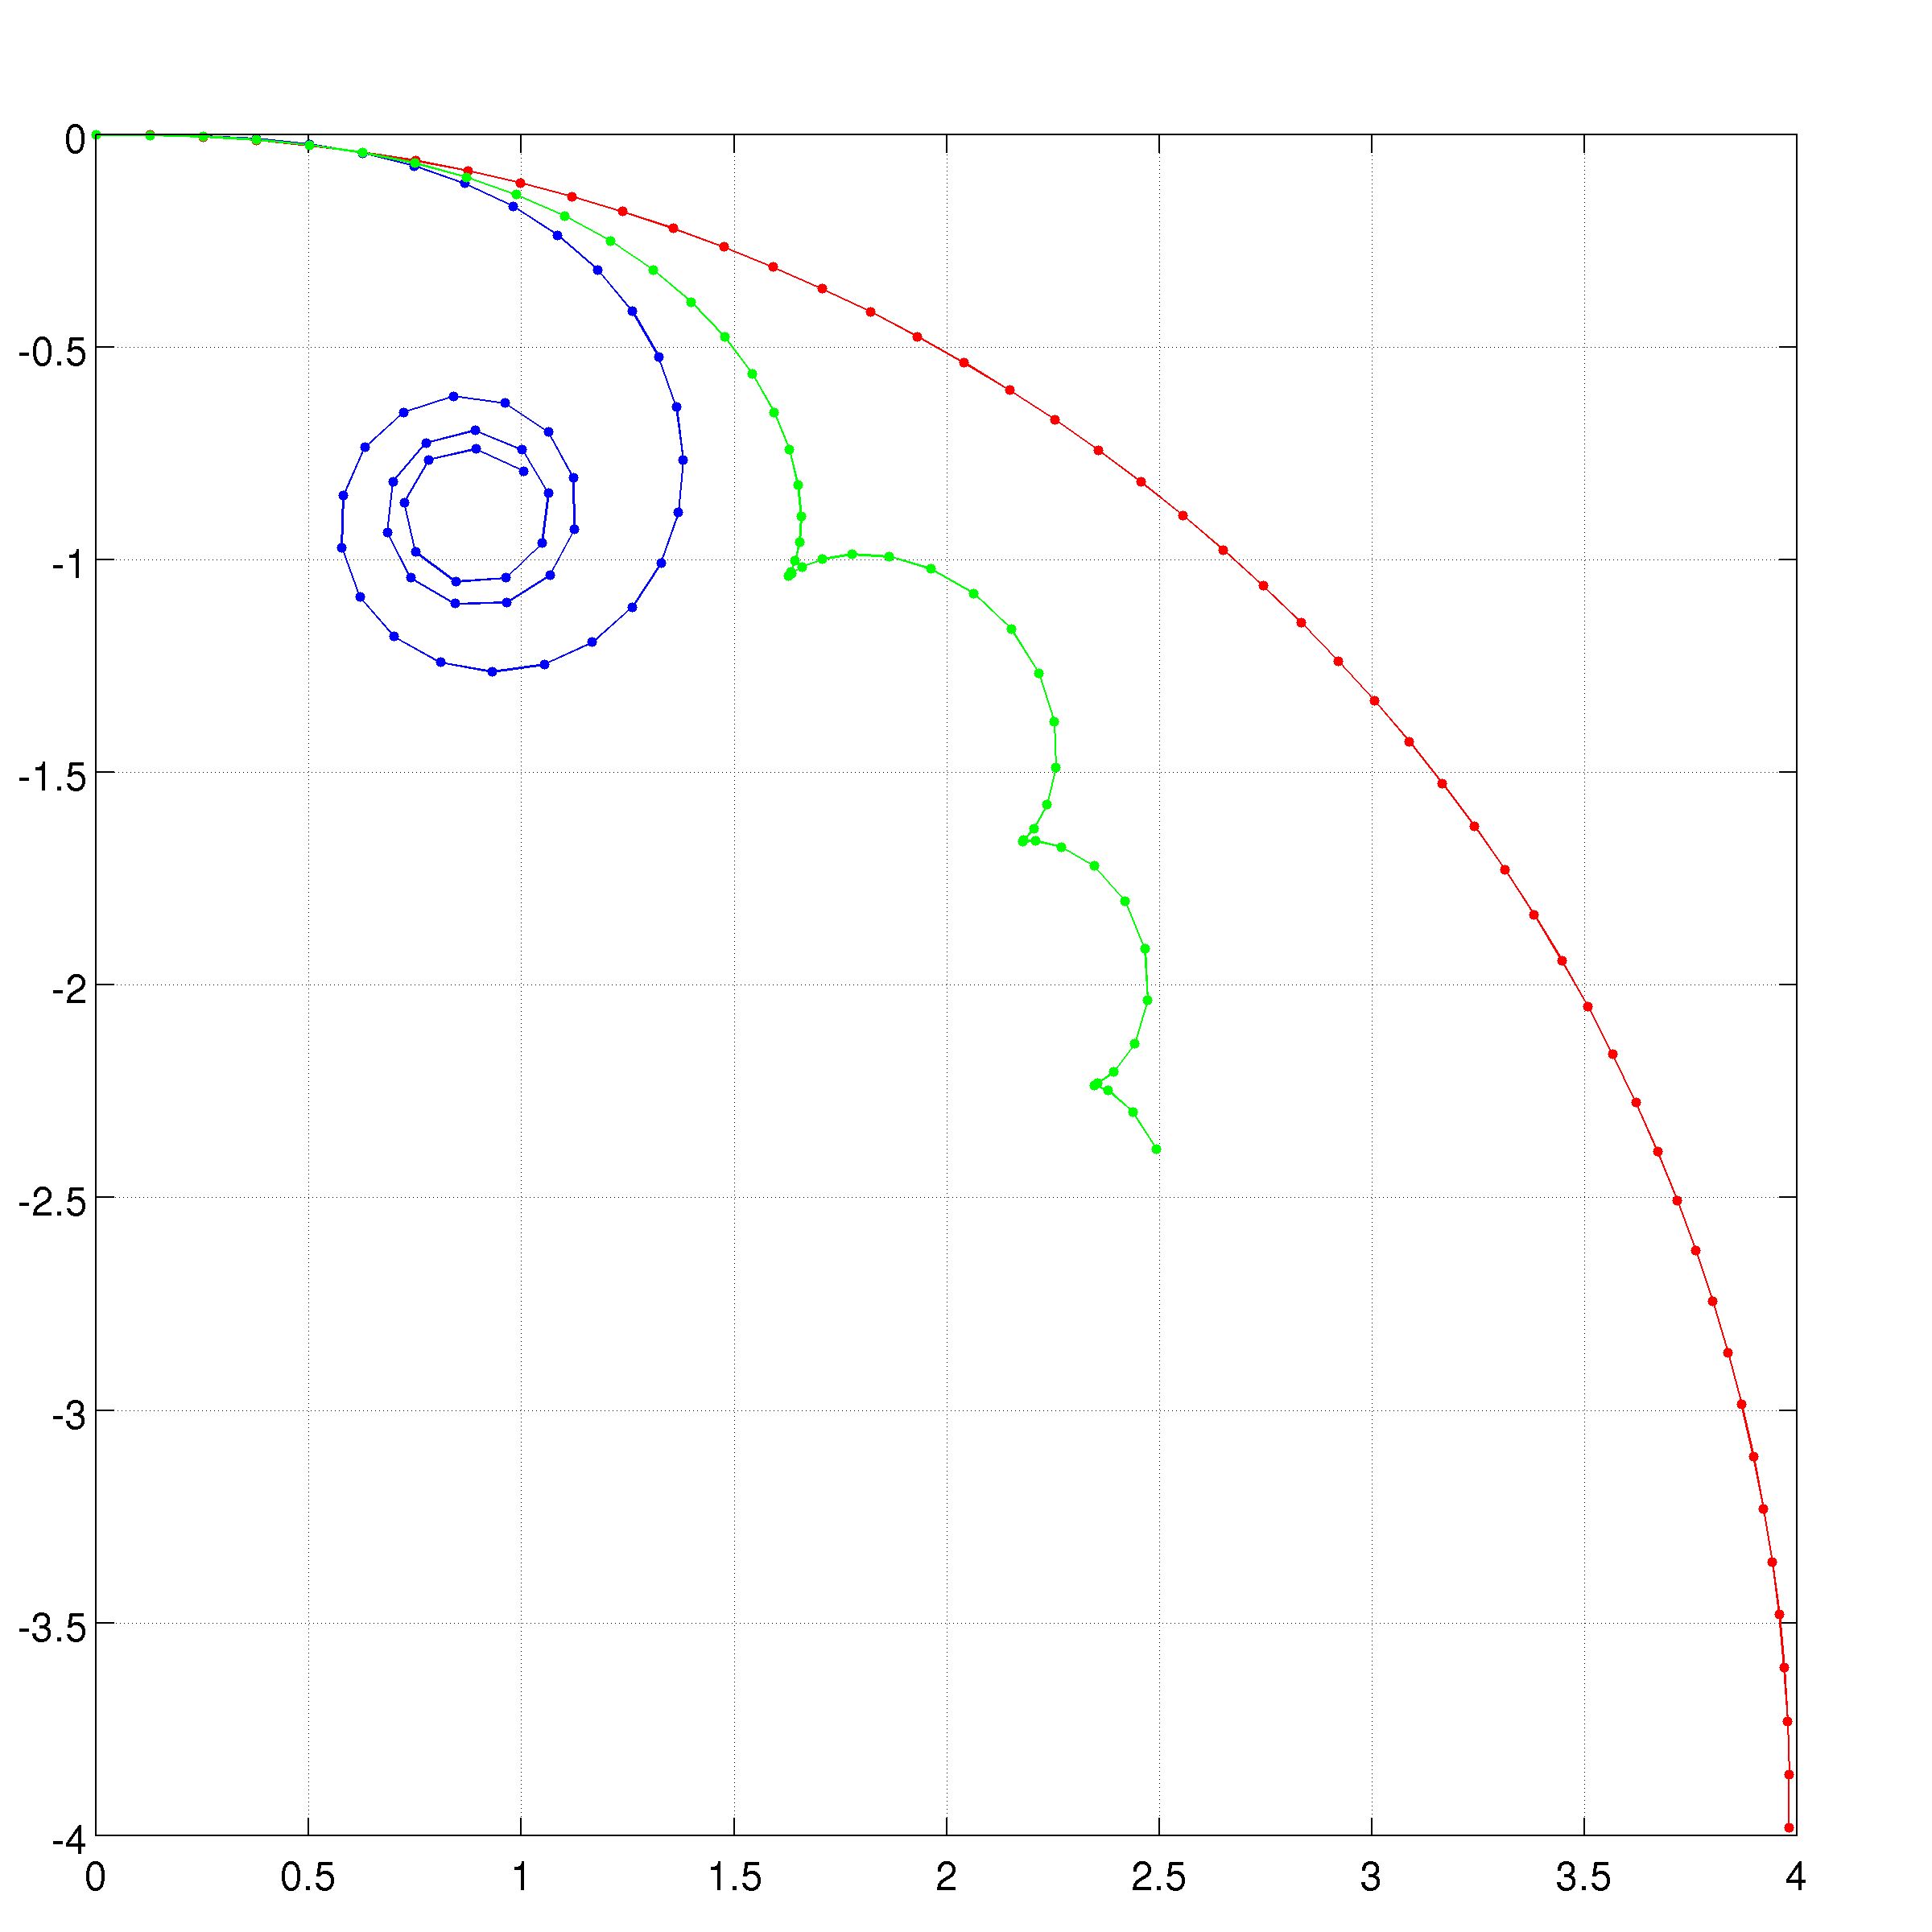
\includegraphics[width=\anchodos]{\chapFiveDir/curves/example_interp_euclidean.png}
		\label{fig:image_interpolation:curve_interpolation:example:euclidean}
	}
	\subfloat[Intrisinc interpolation]{
		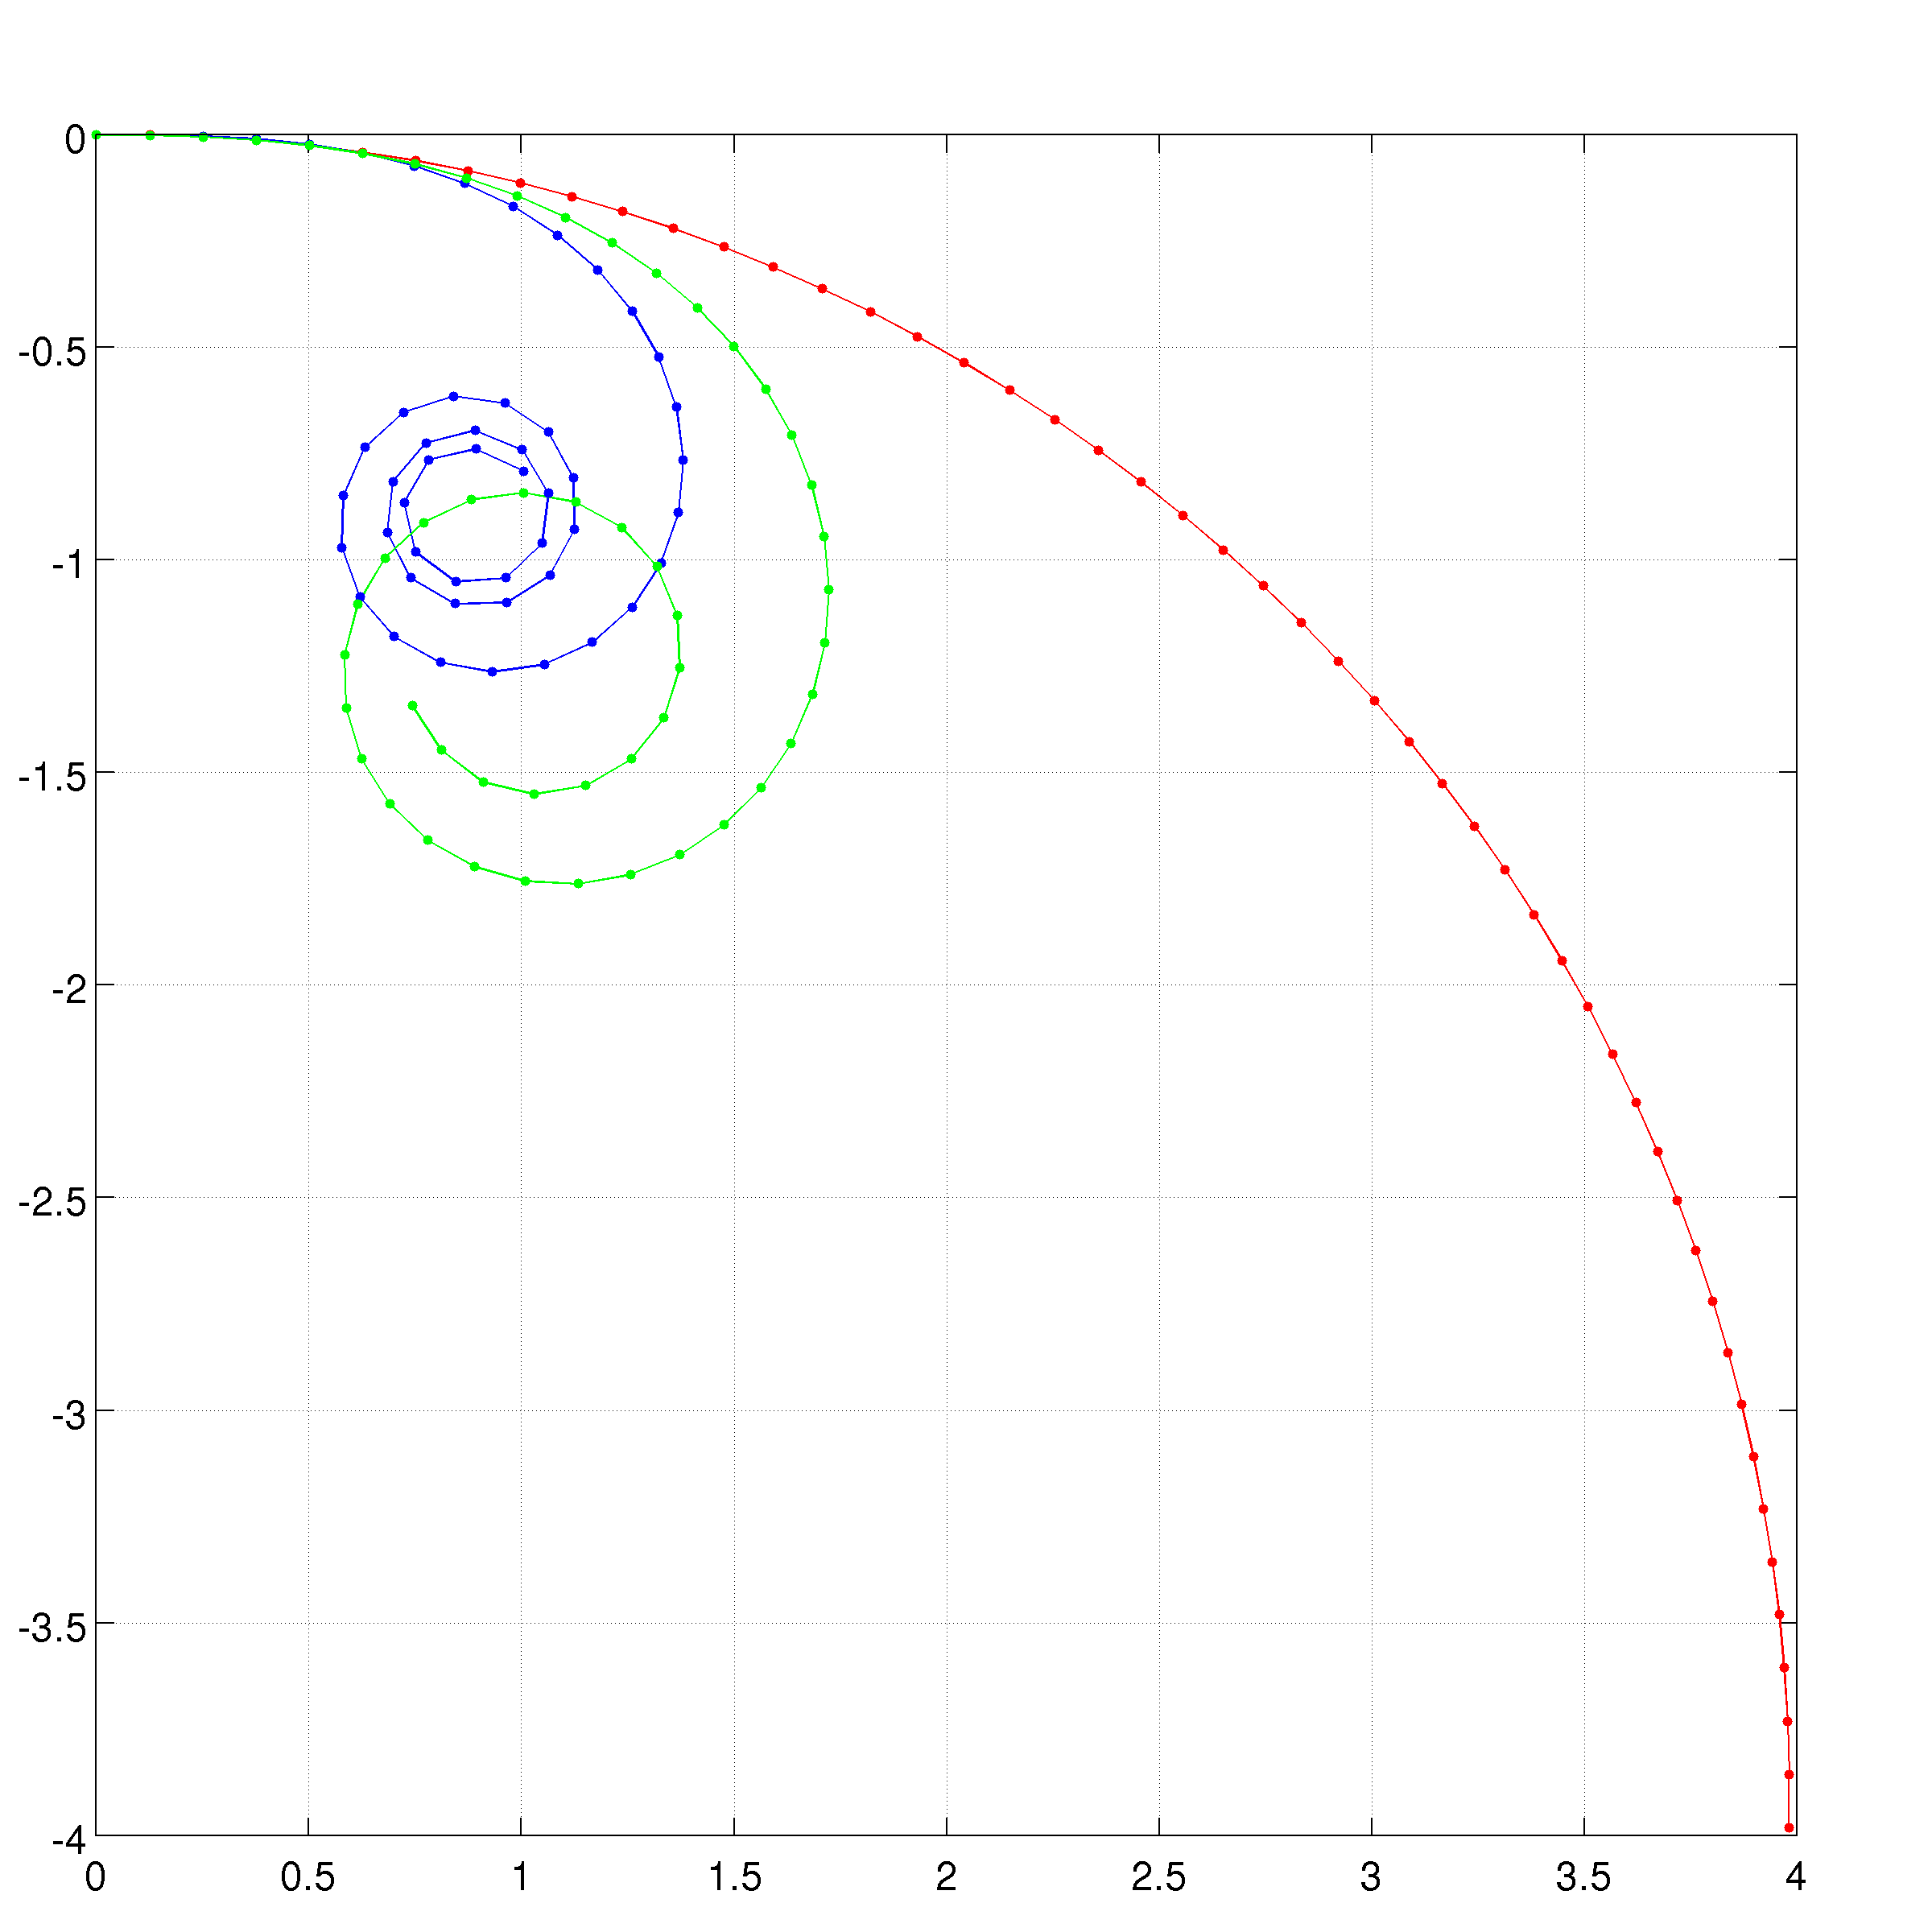
\includegraphics[width=\anchodos]{\chapFiveDir/curves/example_interp_curvature.png}
		\label{fig:image_interpolation:curve_interpolation:example:curvature}
	}
	\caption{Example of two possible choices of curve interpolation. Input curves are depicted in blue and red, and the interpolated curve at $t=0.5$ is depicted in green. \protect\subref{fig:image_interpolation:curve_interpolation:example:euclidean} Interpolation performed directly over the control points. \protect\subref{fig:image_interpolation:curve_interpolation:example:curvature} Interpolation performed only in intrisinc shape parameters. Note how the choice of the interpolation method can greatly affect the results.}
	\label{fig:image_interpolation:curve_interpolation:example}
\end{figure}
%
\section{Introduction}
%
The problem to be addressed in this chapter is the interpolation of two planar curves in a way that respects their intrinsic properties. In this context, we refer to instrinsic parameters as those describing the shape of the curve itself and we label as extrinsic parameters those referring to its global position (rotation, translation, zoom) on a reference system. The literature on this field is vast and a review of the existing approaches is out of the scope of this work. For the sake of this thesis, curve interpolation is only a secondary tool and thus it is enough to find an algorithm that works reasonable well for our applications.
%
One of the main problems of curve interpolation arises when one uses a representation of the curve that mixes extrinsic and intrinsic properties of the curve. This could lead to changes in the intrinsic properties of the curves due to differences in the extrinsic parameters. For instance, linear interpolation on the coordinates of two curves could generate self intersections due to different extrinsic positions of the curves, as depicted in \mbox{Figure \ref{fig:image_interpolation:curve_interpolation:example}} where the initial regular curve completely losses its shape and generates discontinuities. We will call this method Euclidean interpolation.\\

For this reason, we follow the approach presented in \cite{im_proc:curve_interpolation:elber:07:metamorphosis_planar_parametric_curves}, where the authors propose a curve representation that separates intrinsic and extrinsic properties and interpolates them separately. 

In that work, the authors propose a smooth interpolation between two freeform parametric curves, which is carried out by linearly interpolating intrinsic curvature properties. In the following we will review \cite{im_proc:curve_interpolation:elber:07:metamorphosis_planar_parametric_curves}, reproduce its results and show how we extended it to our case of interest.

\section{Curve reconstruction using curvature signatures}\label{sec:curve_interpolation:curve_reconstruction}
\subsection{Computation of curvature signatures}
Let $C(s)$ be an arc-length planar parametric curve, $T(s)$ its unit tangent vector, $N(s)$ its unit normal vector and $\kappa (s)$ its curvature (scalar).\\

The fundamental theorem of differential geometry states that the curvature field $\kappa (s)$ of $C(s)$, parametrized by arc-length, completely determines the curve up to a rigid transformation. In other words, two curves share the same curvature field if and only if one is a rigid transformation of the other.\\

Given a non arc-length parametrized planar curve $C(t)=\left( x(t),y(t) \right)$ the modulus of the tanget field is

\begin{equation}
||C'(t)||=\sqrt{x'^2(t)+y'^2(t)}
\label{eq:image_interpolation:curve_interpolation:velocity}
\end{equation}

And thus, its curvature field $\kappa (t)$ is computed as

\begin{equation}
\kappa (t)=\frac{x'(t)y''(t)-x''(t)y'(t)}{||C'(t)||^3}
\label{eq:image_interpolation:curve_interpolation:curvature}
\end{equation}

where we assumed that $C(t)$ is regular and $||C'(t)||\neq 0$.

In the original paper \cite{im_proc:curve_interpolation:elber:07:metamorphosis_planar_parametric_curves}, the authors are interested in deriving analytical expressions for the curves, which is not the case of the present work. However, for the sake of completeness we review that part of the work.

Parametric curves are often described by polynomial or rational forms which, in general, cannot be reparametrized as closed parametric forms. However as they claim, an arbitrarly precise reparametrization function $t(s)$ can be obtained with tractable algorithms. 
Once $t(s)$ is approximated, we can compute the curvature signature with respect to the new parameter $s$, as $\kappa (s)=\kappa (t(s))$. Using that $s$ is the arc-length of the curve, it holds that $||C'(t)||\approx 1$, thus Equation \ref{eq:image_interpolation:curve_interpolation:curvature} is simplified as follows

\begin{equation}
\kappa (s)=x'(s)y''(s)-x''(s)y'(s)
\label{eq:image_interpolation:curve_interpolation:curvature_reparametrized}
\end{equation}

\begin{figure}[h]
	\centering
	\subfloat[]{
		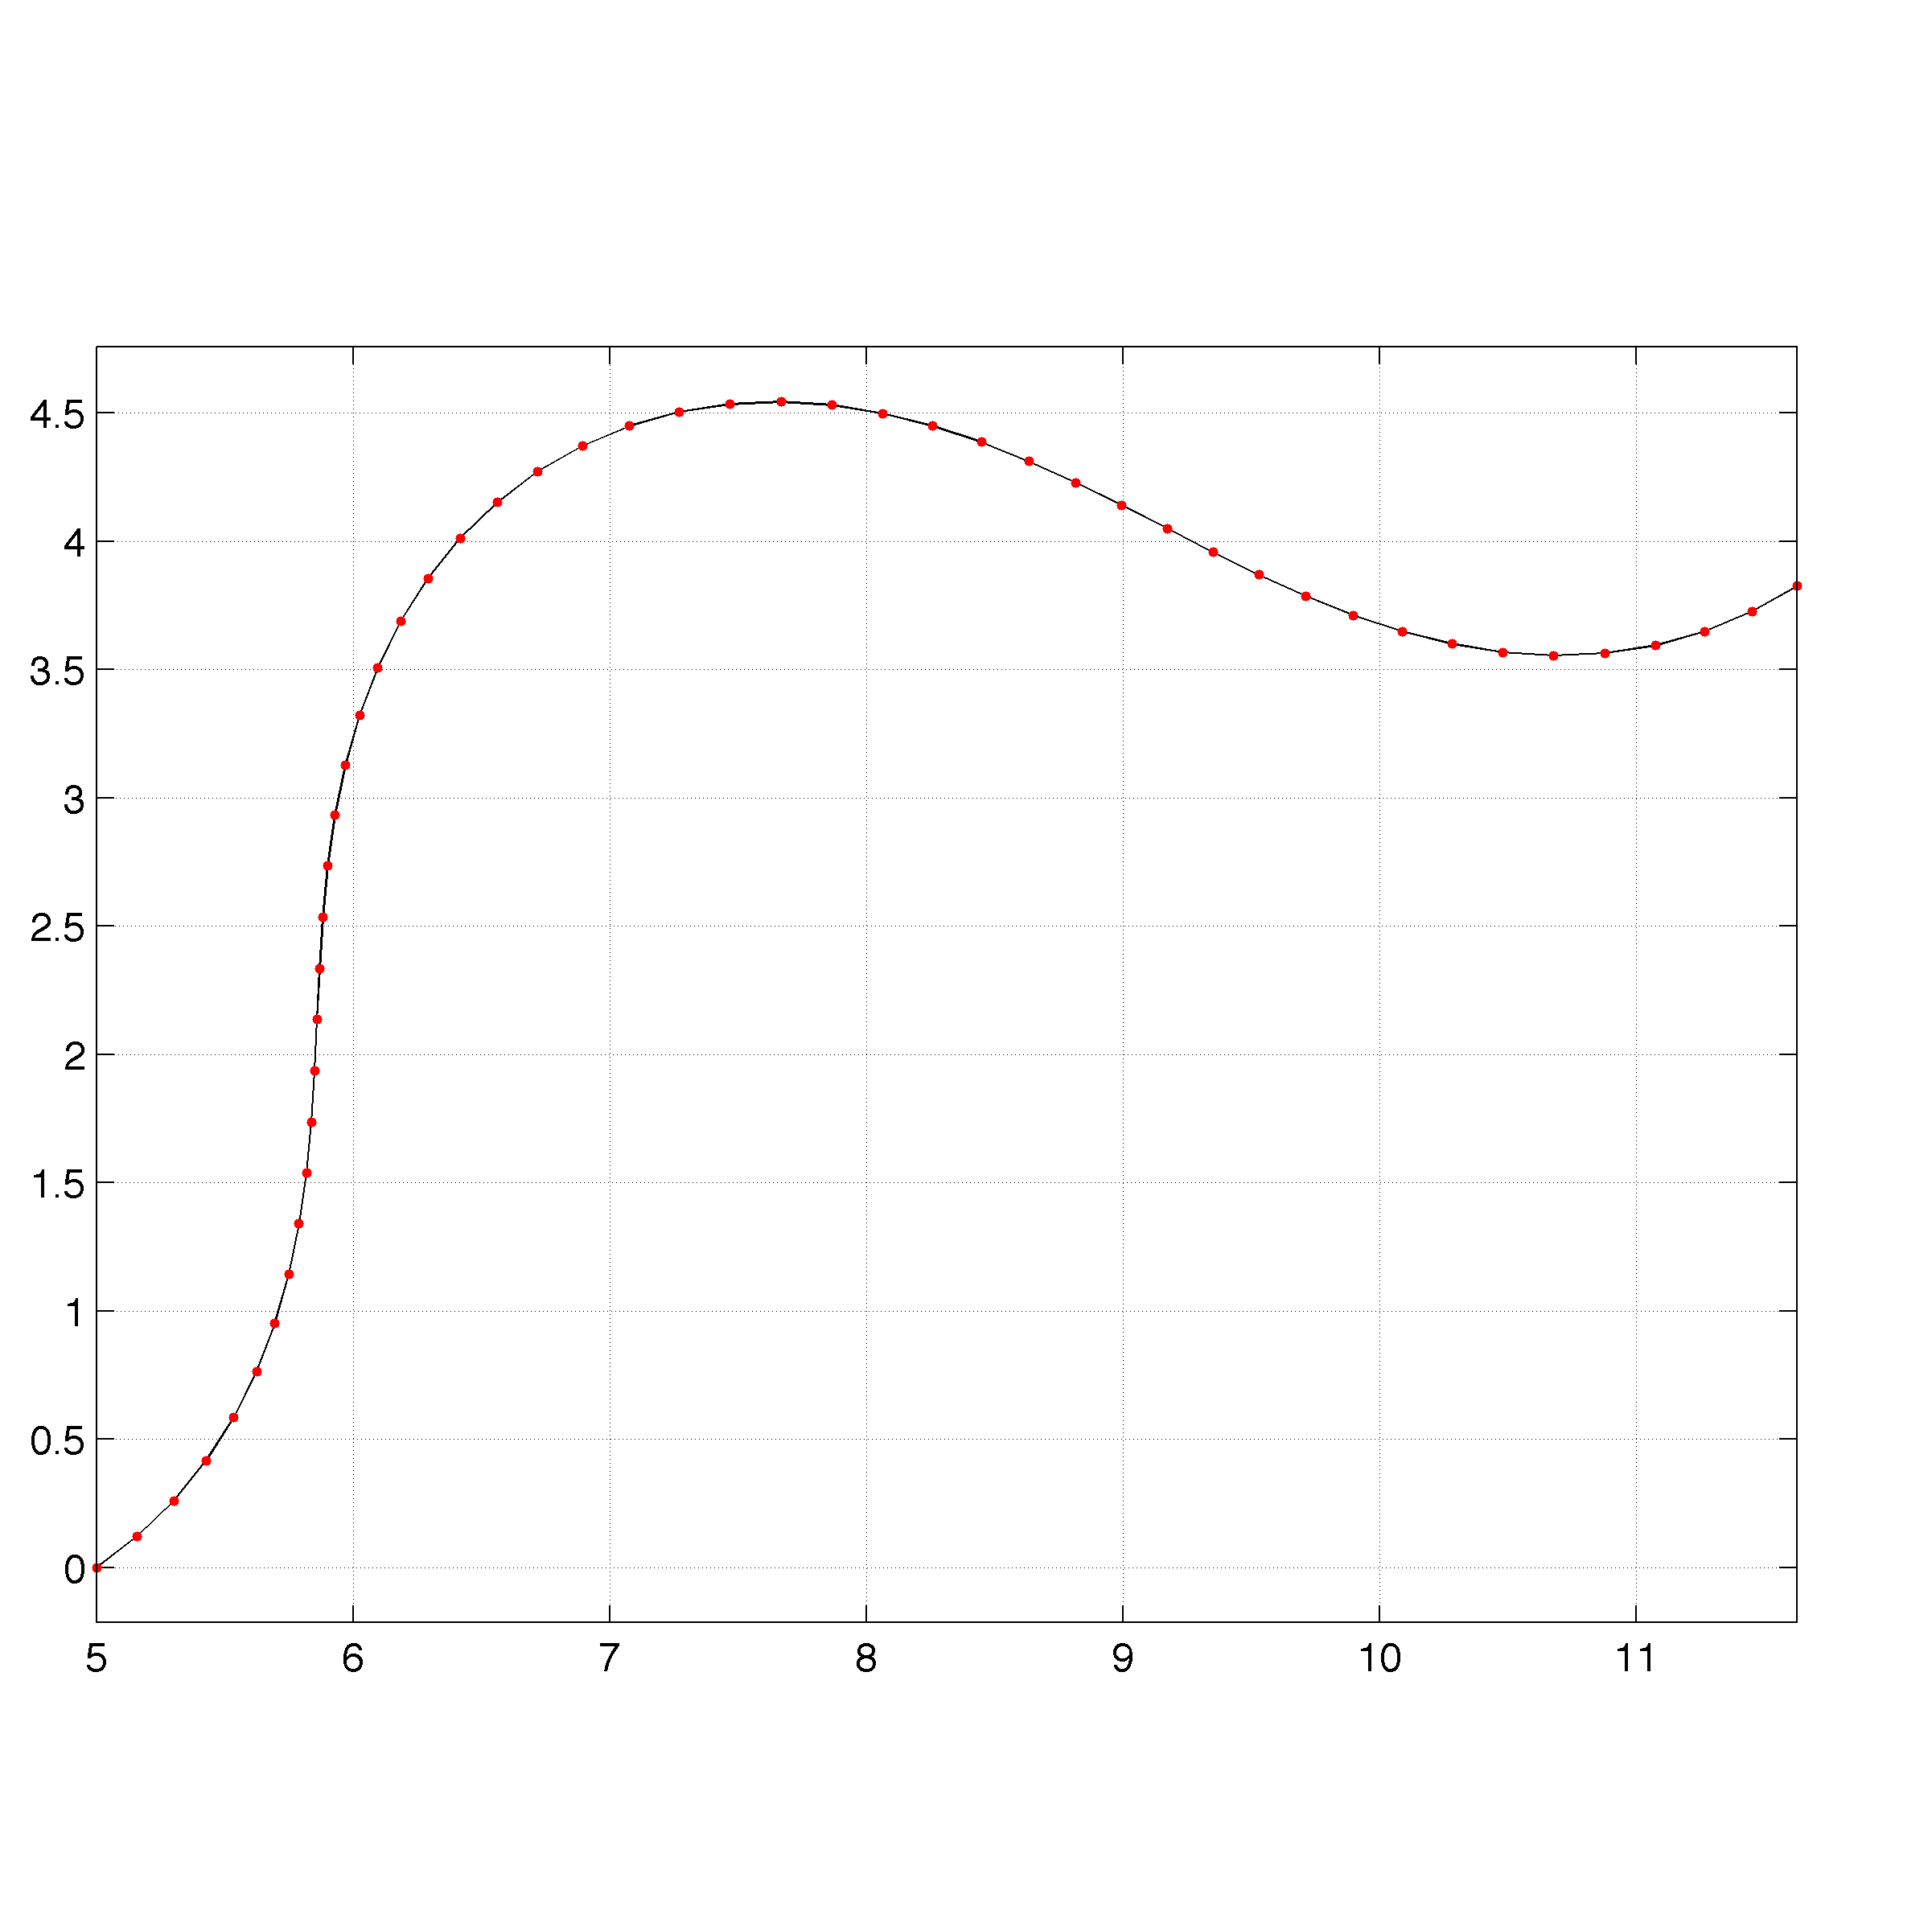
\includegraphics[width=\anchodos]{\chapFiveDir/curves/curve_example_sine_angle}
		\label{fig:image_interpolation:curve_interpolation:input:dense}
	}
	\subfloat[]{
		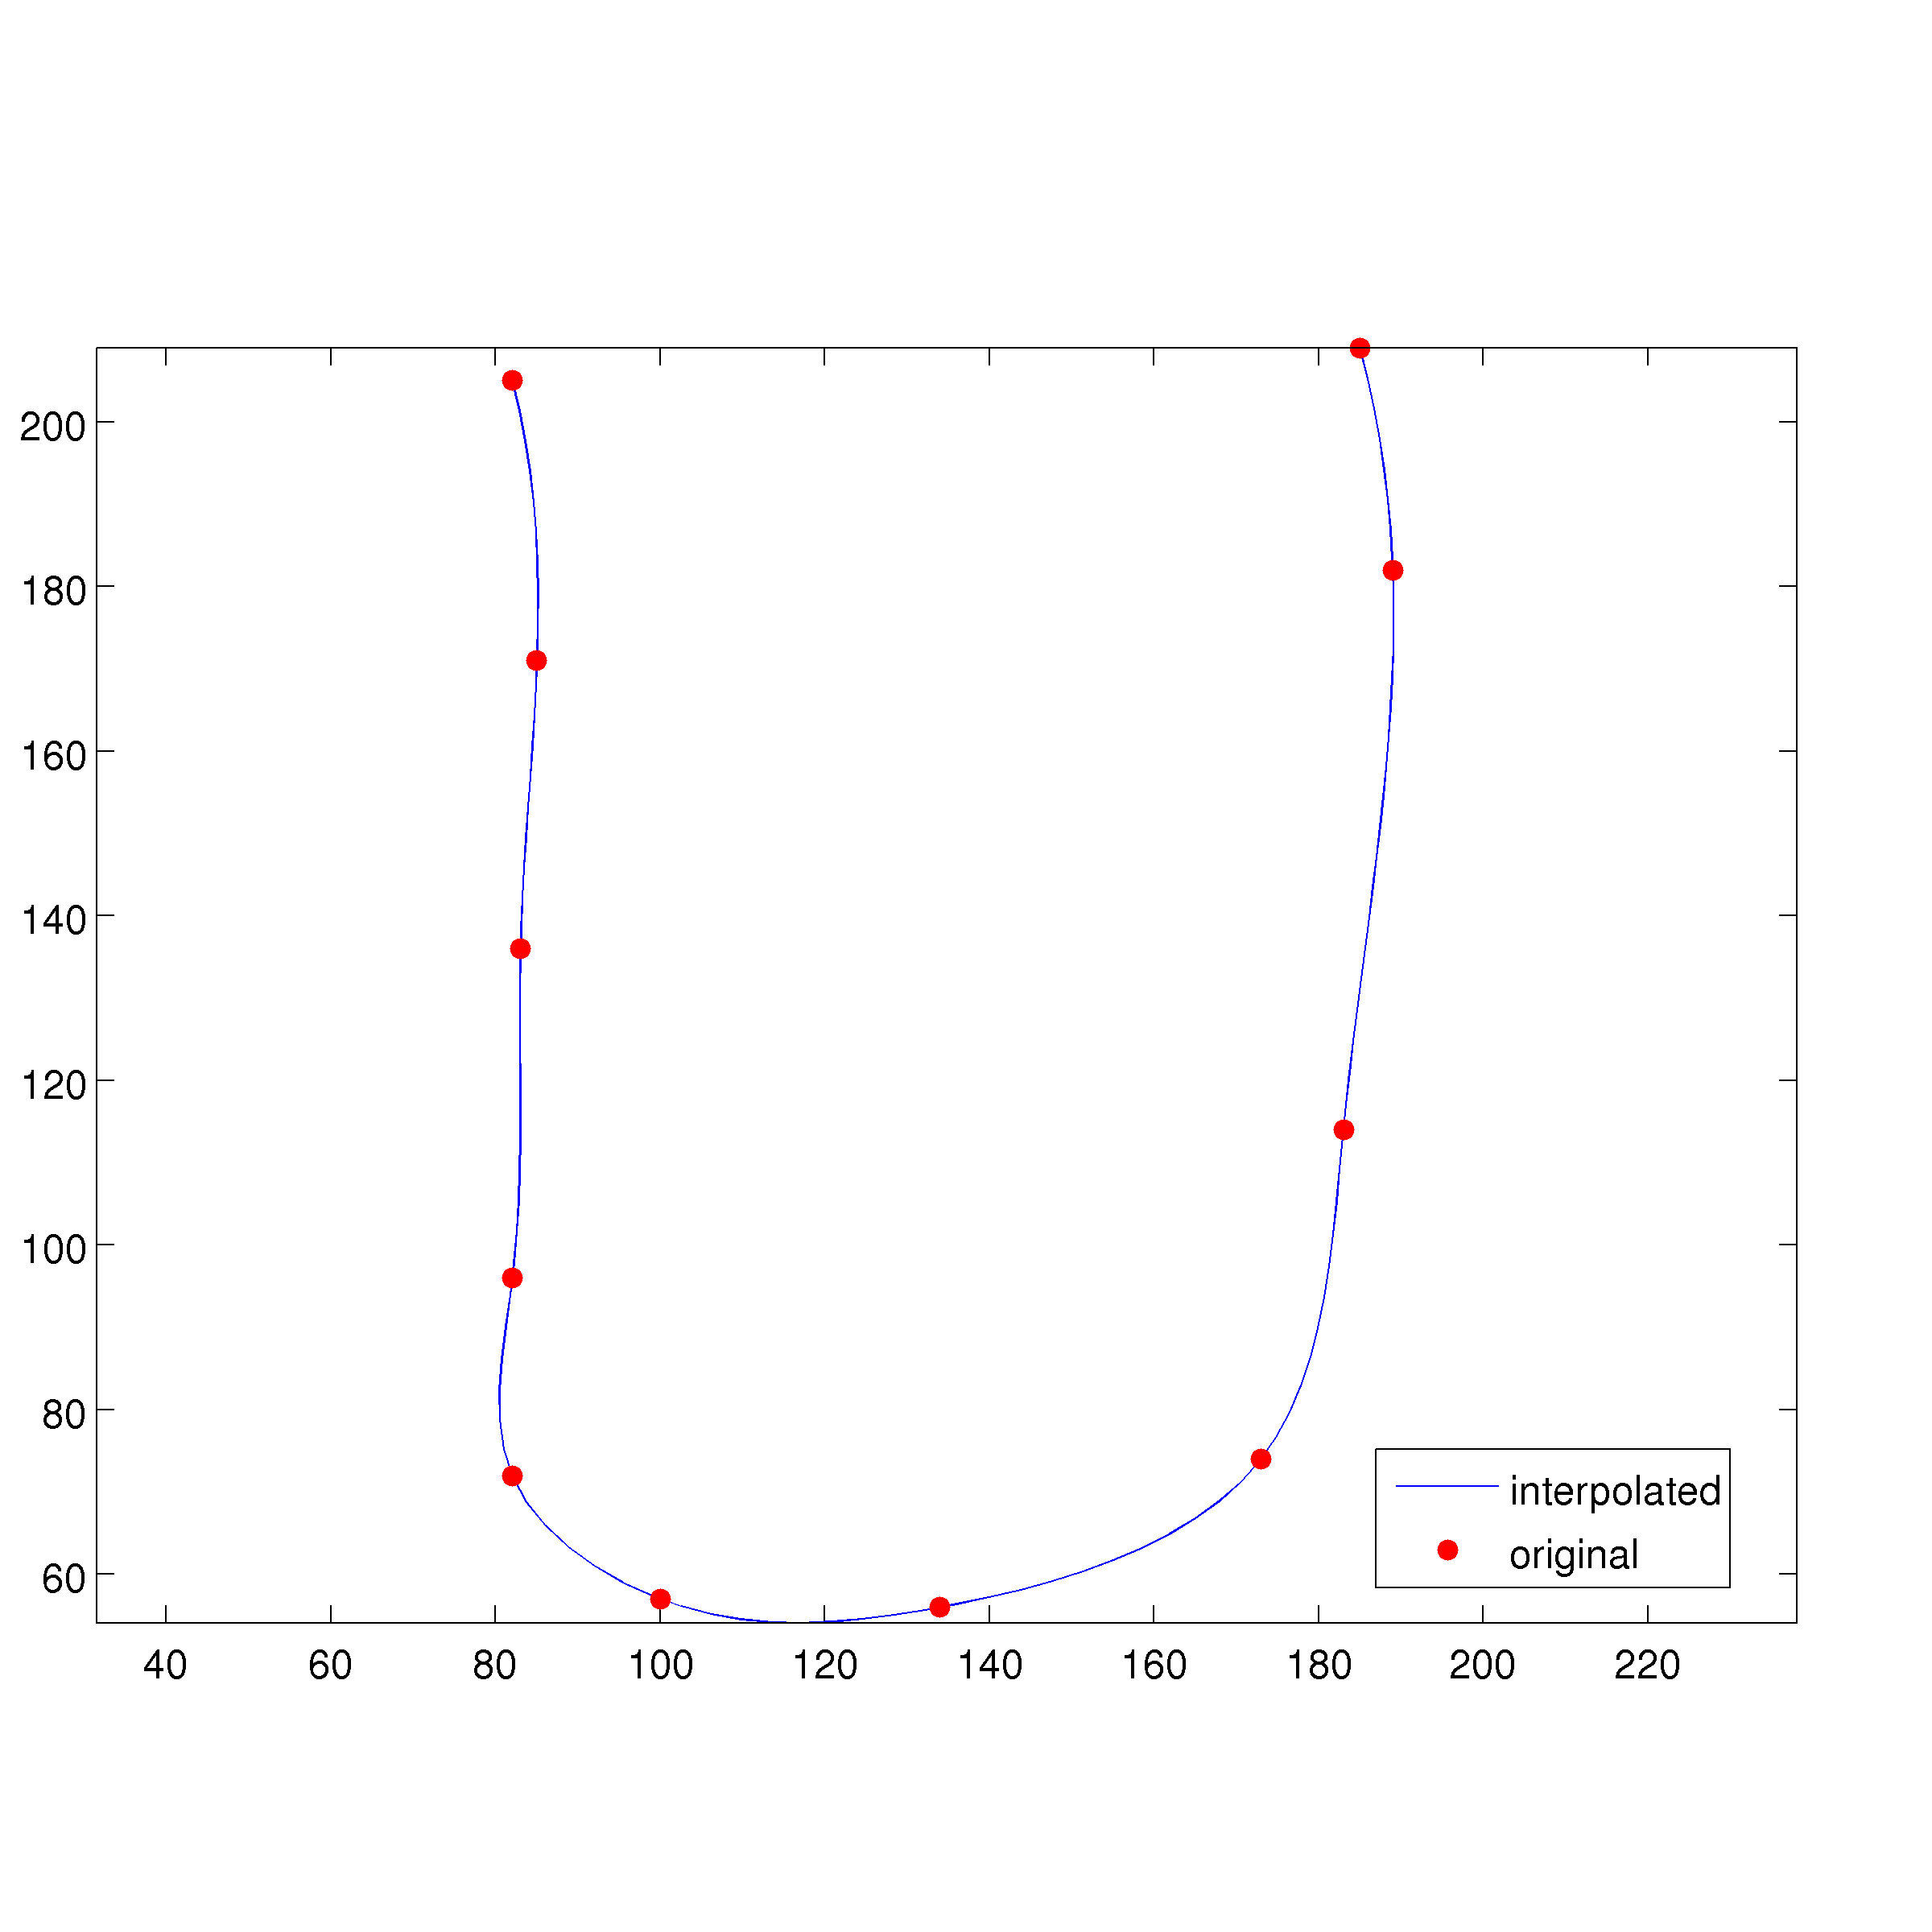
\includegraphics[width=\anchodos]{\chapFiveDir/curves/polyline_interpolated}
		\label{fig:image_interpolation:curve_interpolation:input:control_points}
	}
	\caption{Examples of two possible ways to define input curves used in this work. 
		\protect\subref{fig:image_interpolation:curve_interpolation:input:dense} Dense curve obtained by regular sampling of its analytical expression.
		\protect\subref{fig:image_interpolation:curve_interpolation:input:control_points} Original polyline (red dots) composed of sparse control points and its dense approximation using interpolation (blue line). }
	\label{fig:image_interpolation:curve_interpolation:input}
\end{figure}

In our case, the input will be discrete curves which could be obtained in two ways: 
\begin{itemize}
 \item Sampling: In this case the discrete curve will be a correct (dense) sampling of a continuous unknown curve. Thus, we will have a dense sampling of the curve and we will be able to directly compute differential magnitudes using standard finite differences.
 \item Control points: In this case, the curve will be represented as a few key points used to control the behavior of the curve. Thus, we will have a very sparse representation of the curve from which we are not able to compute differential magnitudes.
\end{itemize}

These two cases are depicted in Figure \ref{fig:image_interpolation:curve_interpolation:input} where an example of a dense sampling and a sparse representation are shown.

We will start with the simpler case of a dense curve and then extend it to a sparse one.

In the dense case of Figure \ref{fig:image_interpolation:curve_interpolation:input:dense} the curve is regularly sampled, but not parametrized by arc length. For this curve, we show in Figure \ref{fig:image_interpolation:curve_interpolation:normals} the normal and tangent vector fields computed used first order finite differences. As Figure \ref{fig:image_interpolation:curve_interpolation:normals:mod_vel} shows, the modulus of the tangent field is not exactly unit, but it is very close, so we can use this parametrization as a reasonable approximation of the arc-length parametrization. %\tcom{Se podría mejorar la figura de la norma de la velocidad}

\begin{figure}[h]
	\centering
	\subfloat[]{
		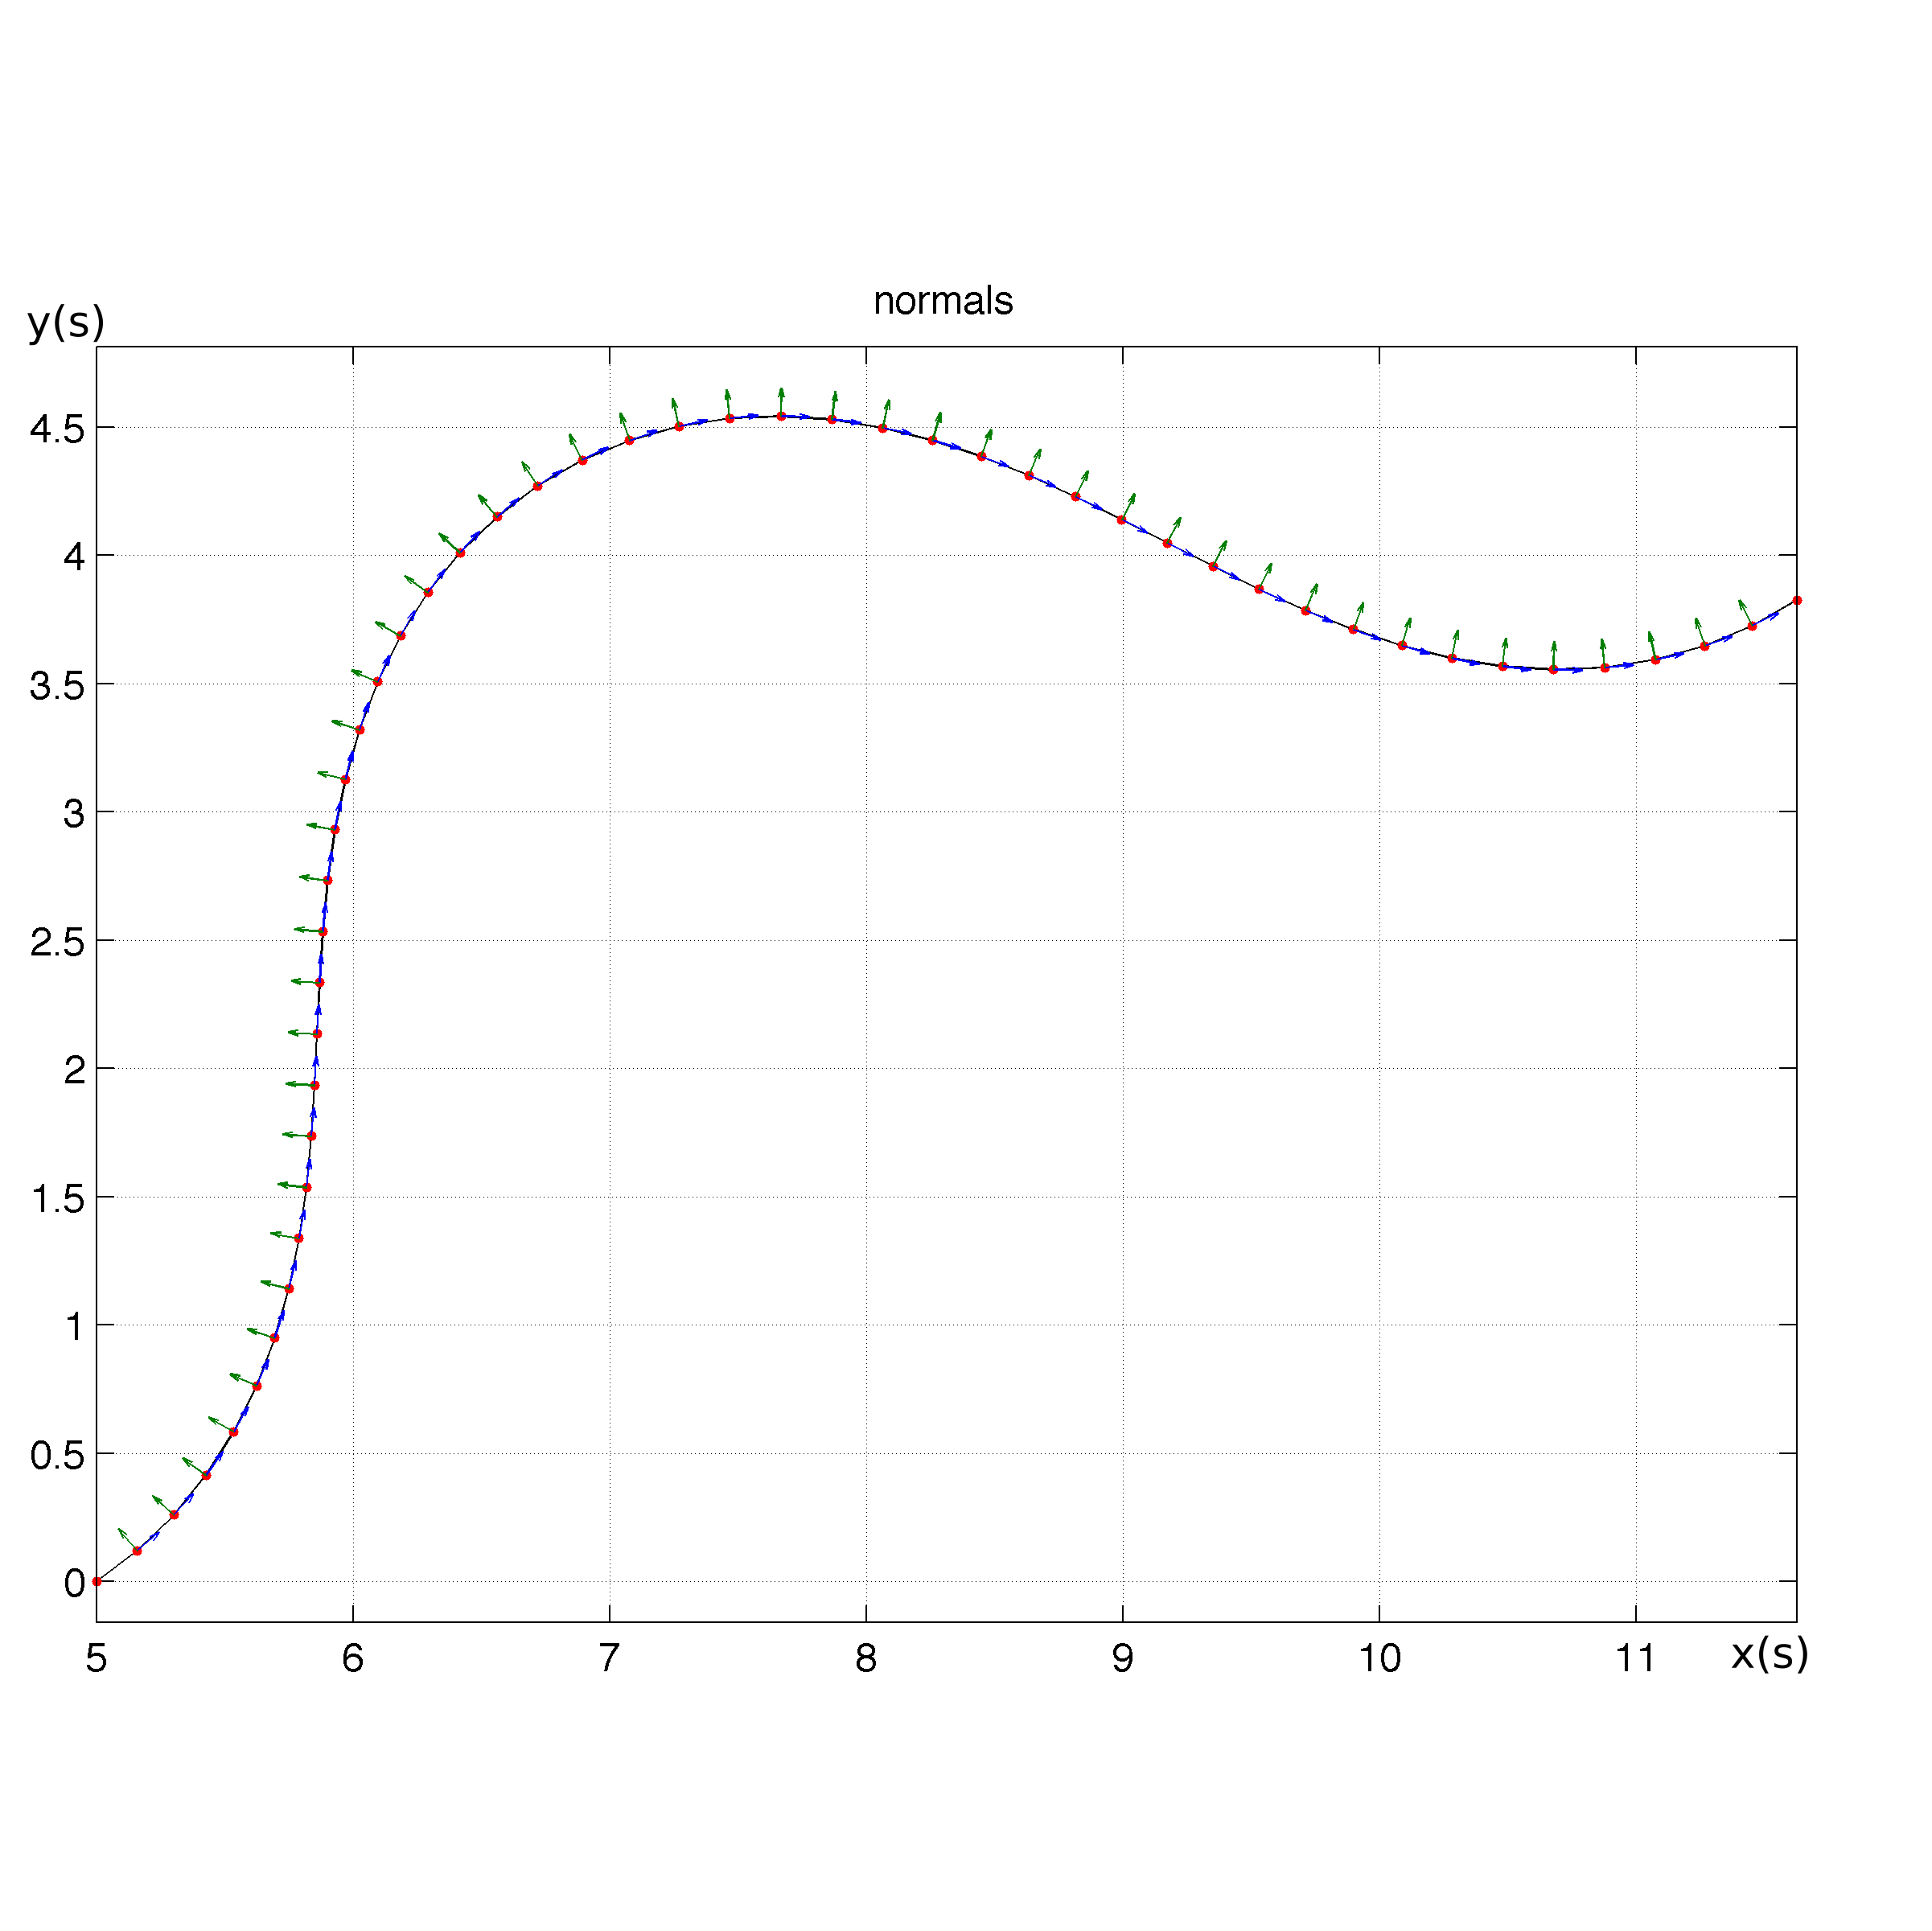
\includegraphics[width=8cm]{\chapFiveDir/curves/curve_normals_edited}
		\label{fig:image_interpolation:curve_interpolation:normals:normals}
	}\\
	\subfloat[]{
		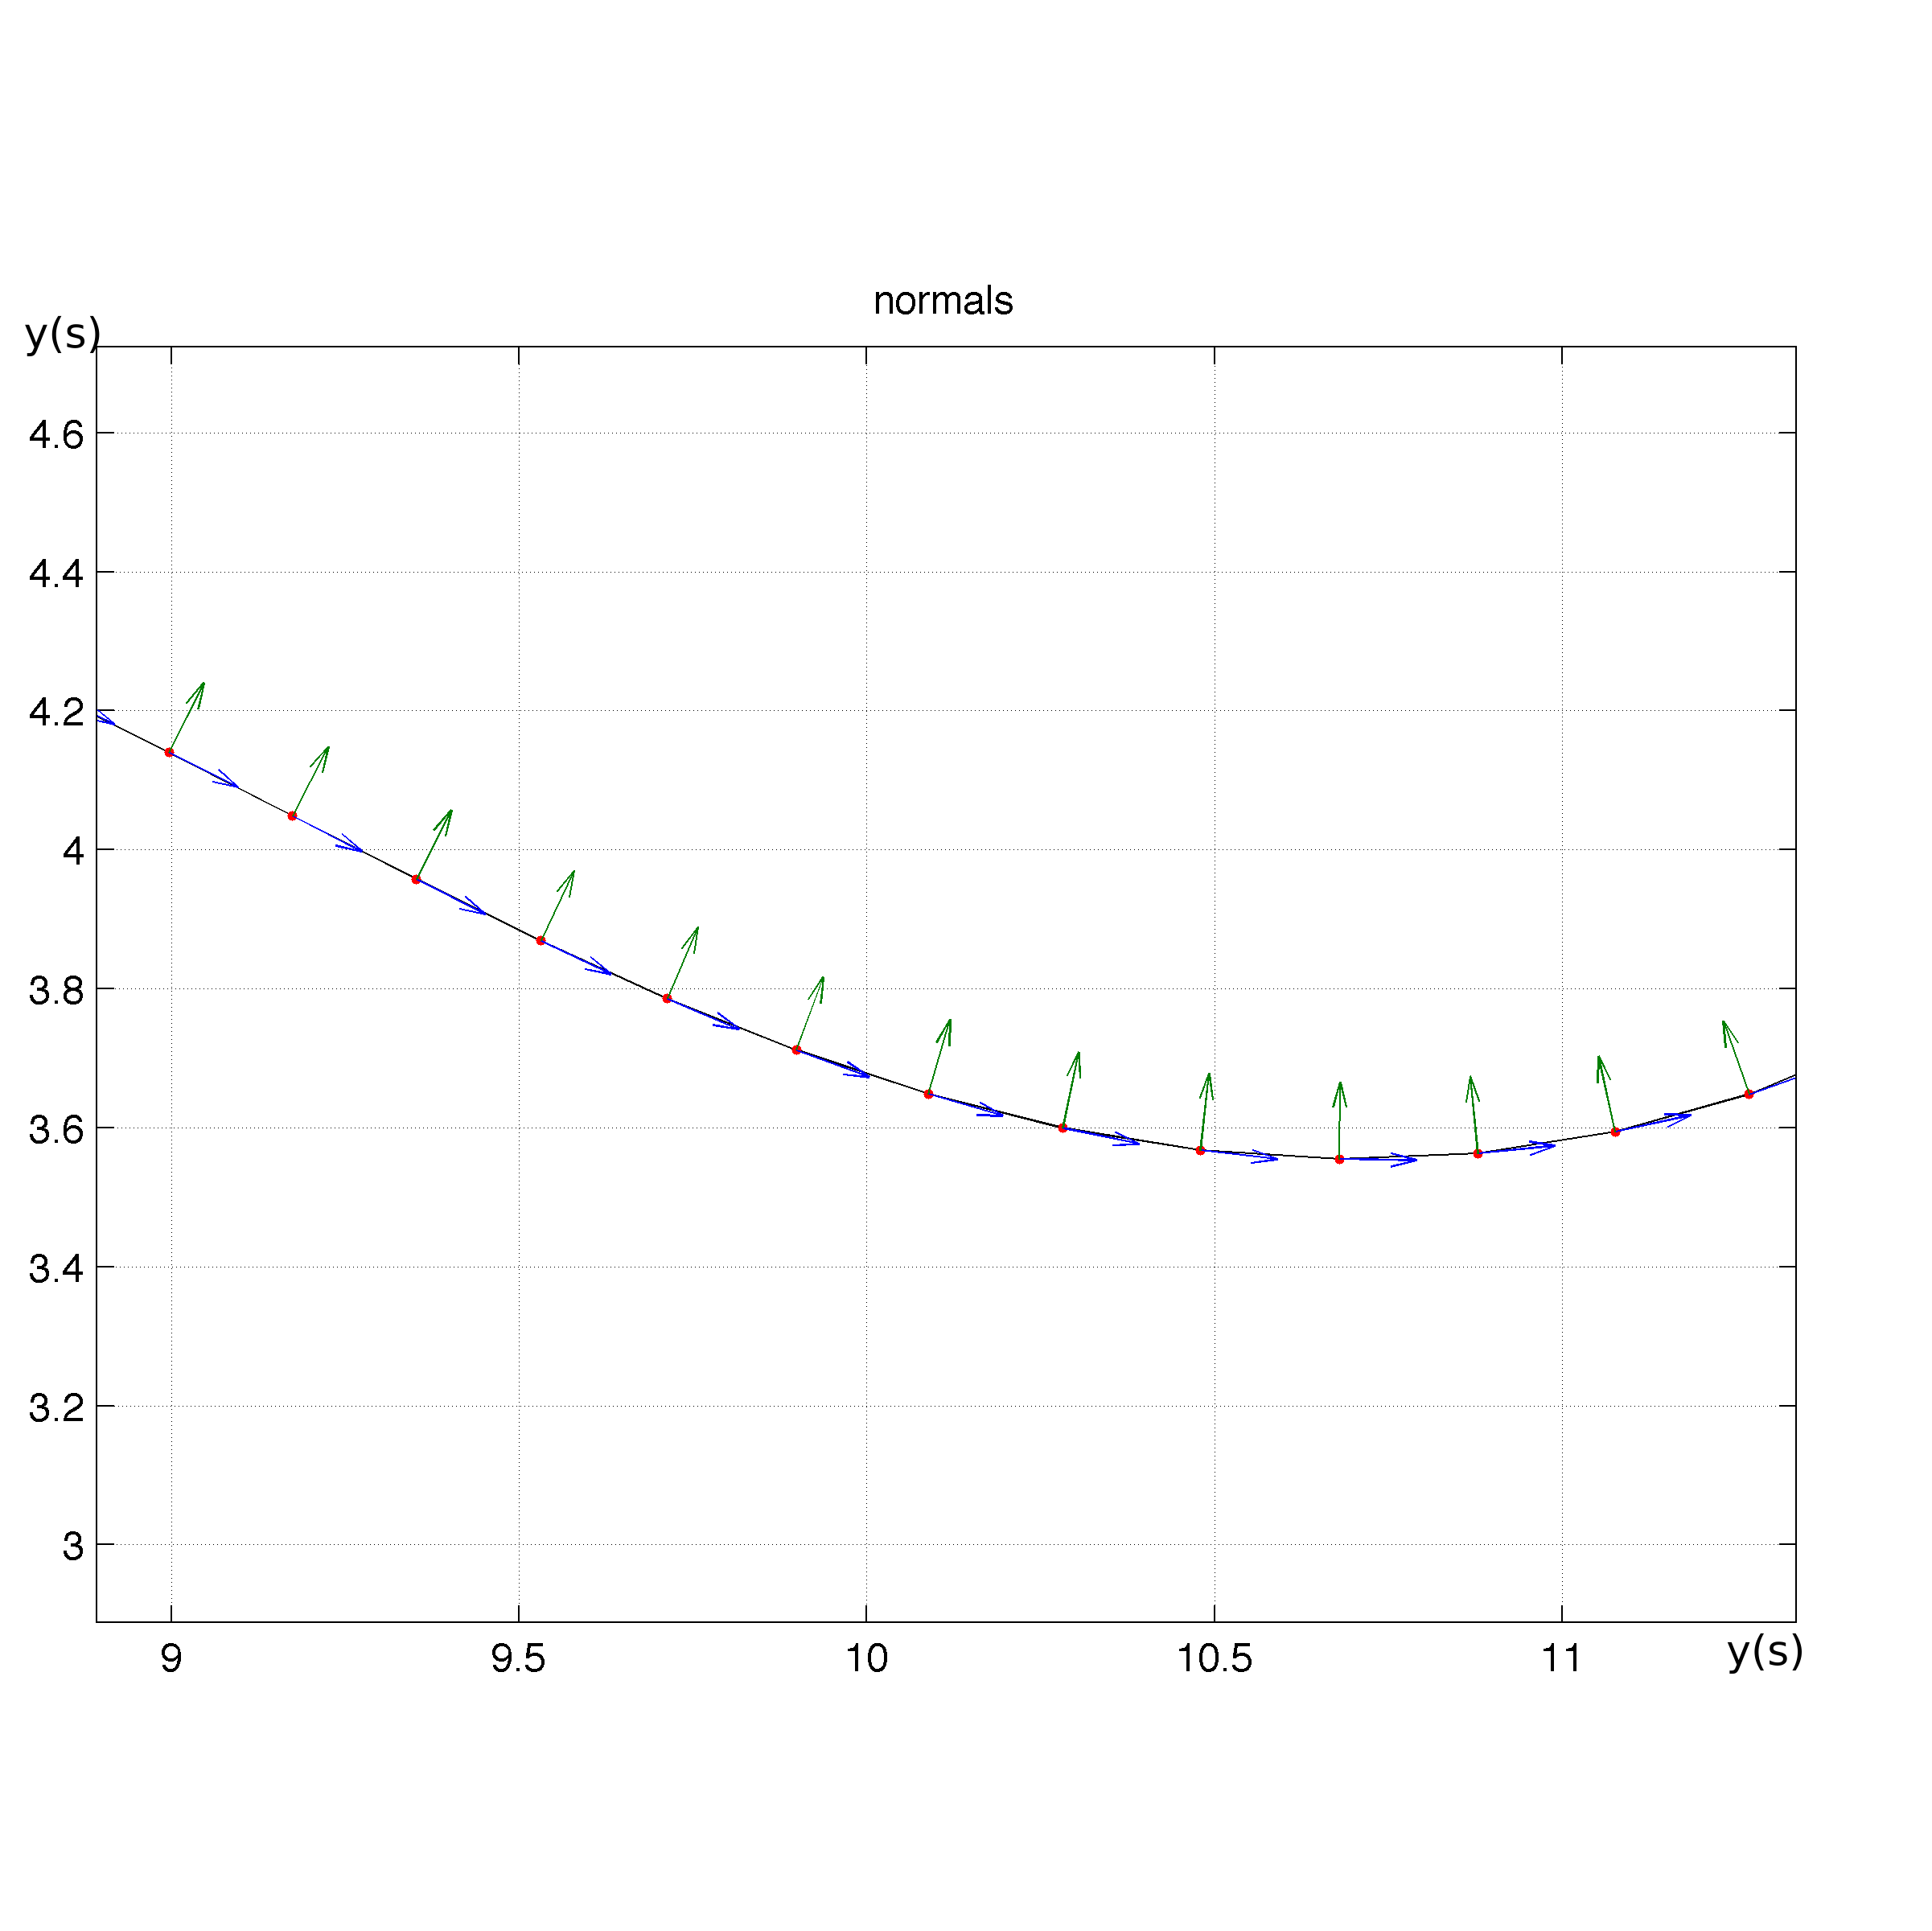
\includegraphics[width=6.5cm]{\chapFiveDir/curves/curve_normals_detail_edited}
		\label{fig:image_interpolation:curve_interpolation:normals:detail}
	}
	\subfloat[]{
	\raisebox{0.13\height}{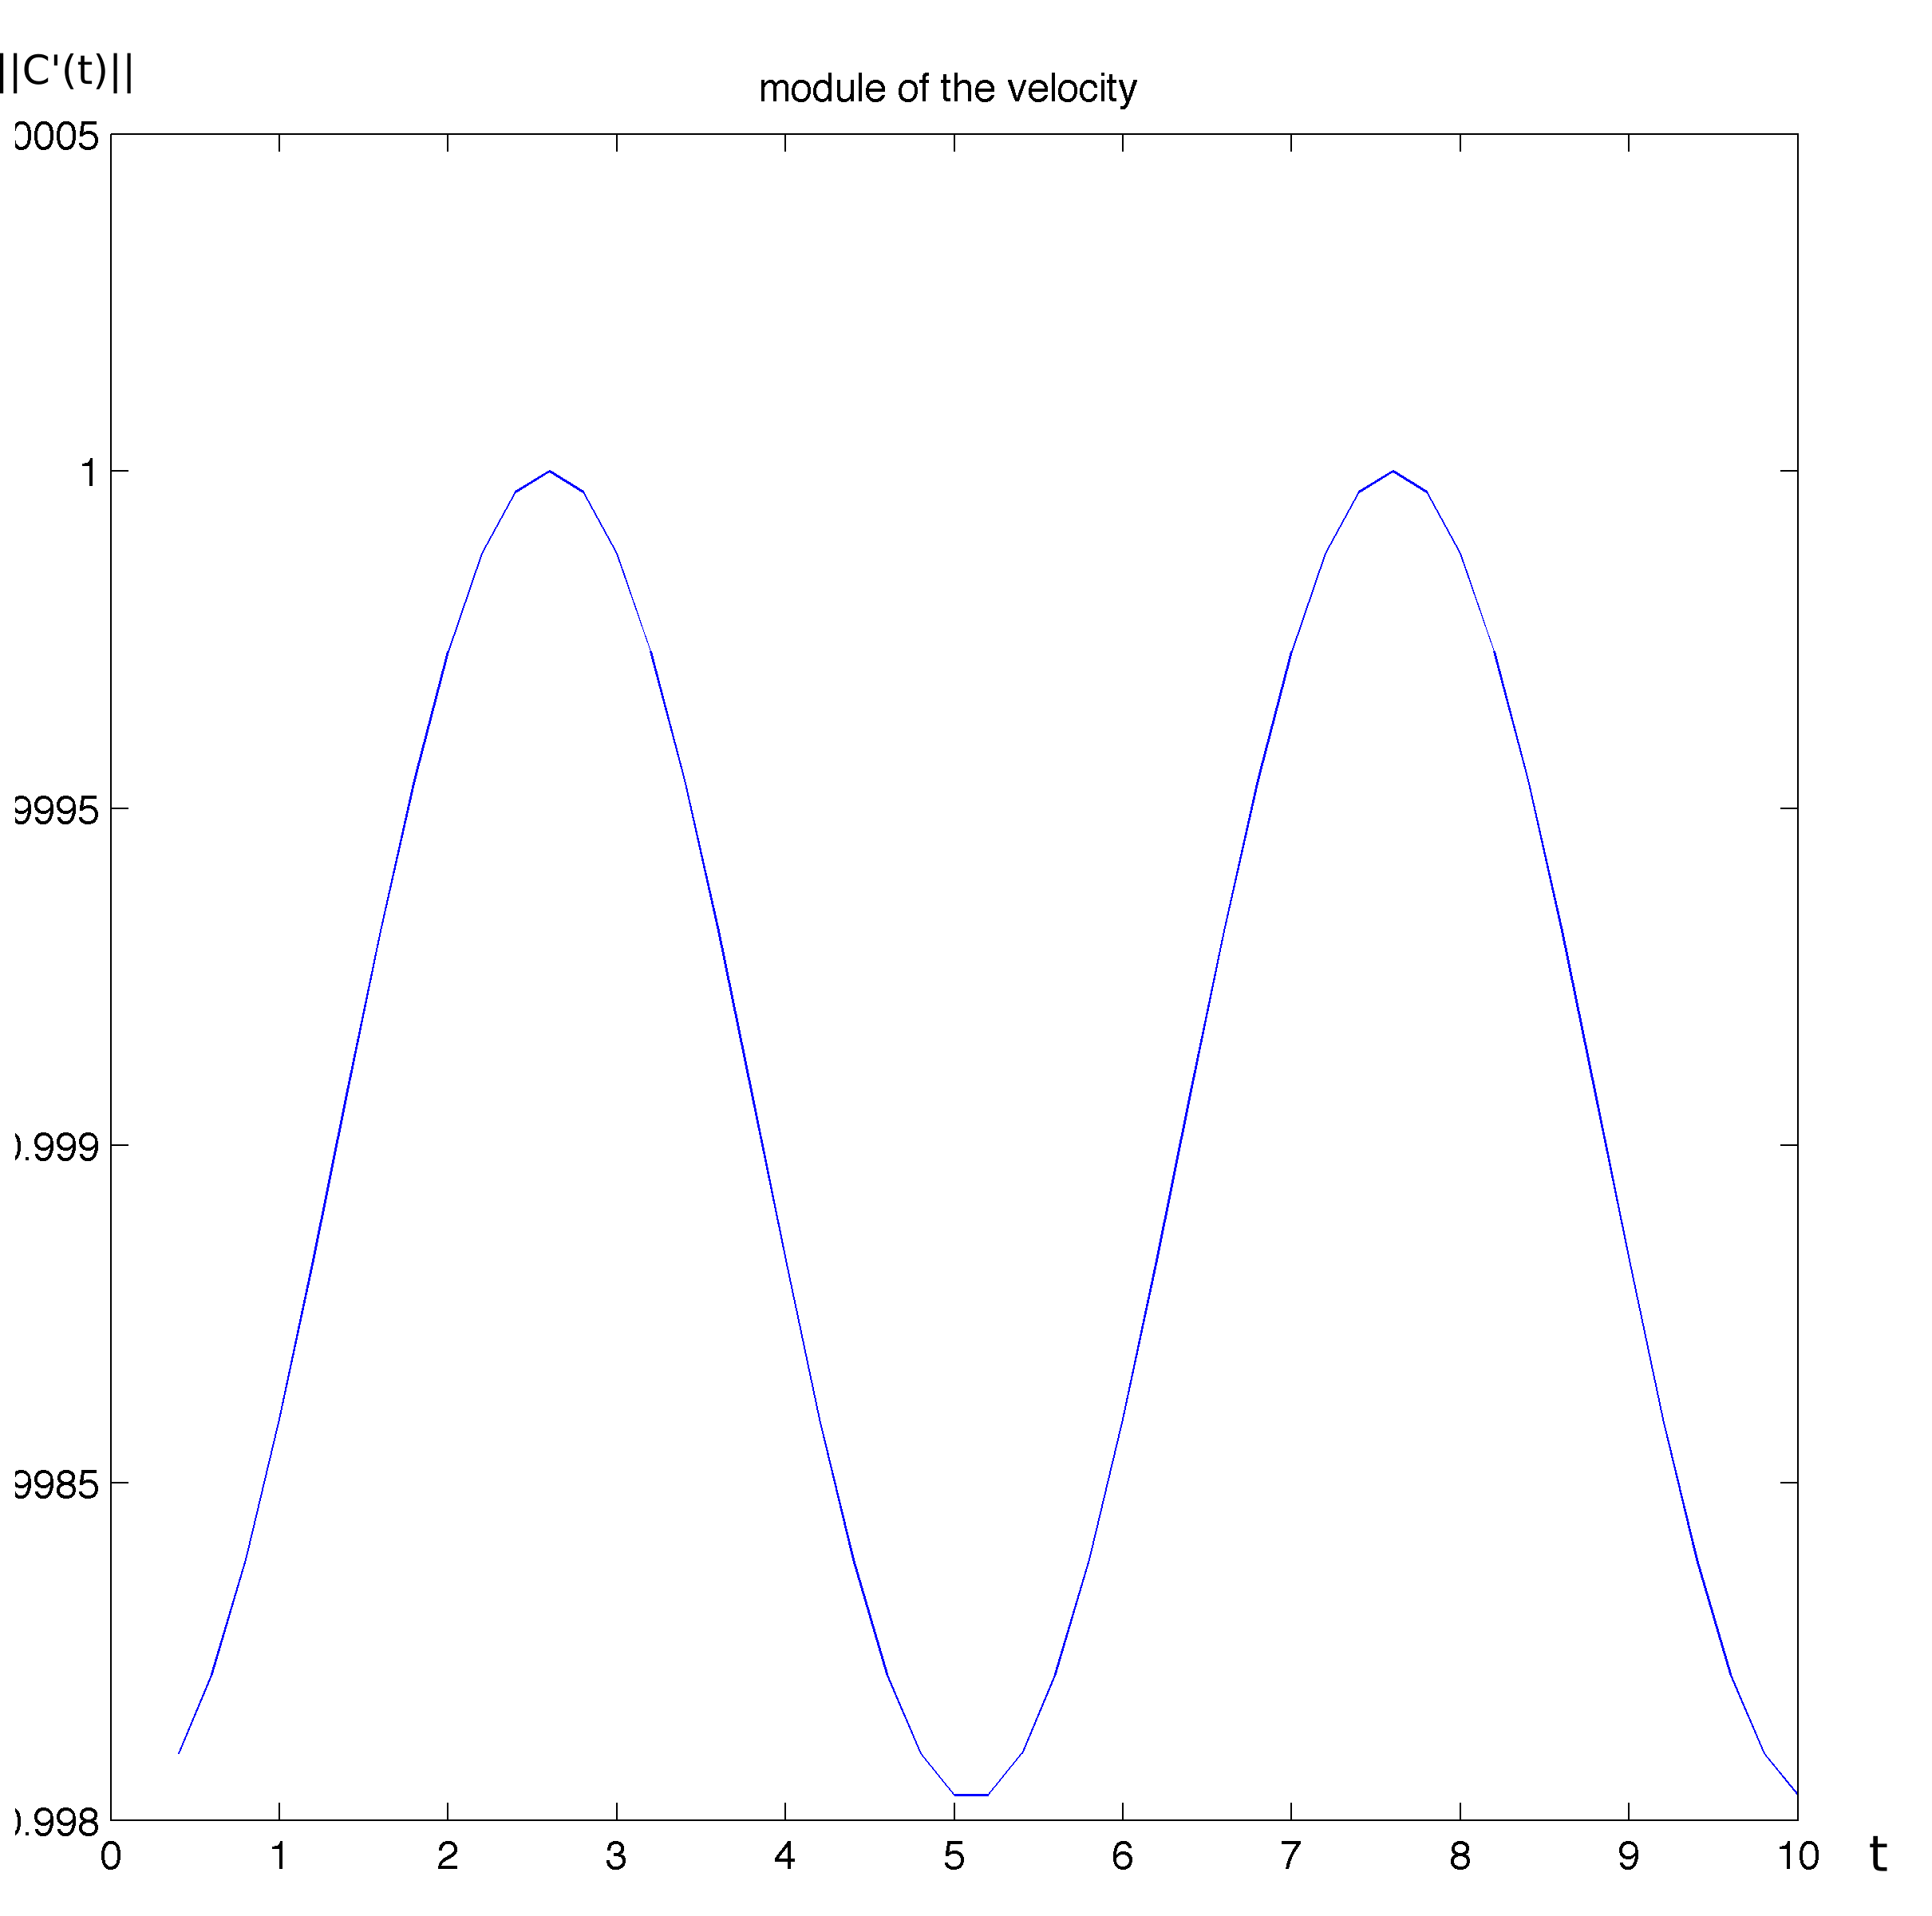
\includegraphics[width=5cm]{\chapFiveDir/curves/curve_mod_vel_edited}}
		\label{fig:image_interpolation:curve_interpolation:normals:mod_vel}
	}
	\caption{
		First order differential magnitudes computed over an example curve.
		\protect\subref{fig:image_interpolation:curve_interpolation:normals:normals} Normal and tangent vector fields of the complete curve.
		\protect\subref{fig:image_interpolation:curve_interpolation:normals:detail} Zoom in of the last part of the curve. 
		\protect\subref{fig:image_interpolation:curve_interpolation:normals:mod_vel} Modulus of the velocity field plotted against parameter $s$.
	}
	\label{fig:image_interpolation:curve_interpolation:normals}

\end{figure}

In Figure \ref{fig:image_interpolation:curve_interpolation:curvature} we show the curvature signature $k(s)$, and we can verify that it completely describes the shape of the curve. The curve starts with positive curvature, until it reaches a saddle point, which can be seen at the zero crossing of the signature shown in Figure \ref{fig:image_interpolation:curve_interpolation:curvature:signature}. In the spatial representation shown in Figure  \ref{fig:image_interpolation:curve_interpolation:curvature:spatial} this can be seen as the vector field initially pointing outwards the curve, then diminishing its module until it changes direction at the saddle point.

\begin{figure}[h]
	\centering
	\subfloat[]{
		\includegraphics[width=\anchounoymedio]{\chapFiveDir/curves/curve_curvature_spatial_edited}
		\label{fig:image_interpolation:curve_interpolation:curvature:spatial}
	}
	\subfloat[]{
		\raisebox{0.15\height}{\includegraphics[width=\anchodos]{\chapFiveDir/curves/curve_curvature_edited}}
		\label{fig:image_interpolation:curve_interpolation:curvature:signature}
	}
	\caption{Curvature field computed over our example curve.
		\protect\subref{fig:image_interpolation:curve_interpolation:curvature:spatial} Spatial representation, where curvature is represented as a normal vector with length proportional to its value, i.e. $C''(s)=\kappa(s)N(s)$.
		\protect\subref{fig:image_interpolation:curve_interpolation:curvature:signature} Curvature plotted against curve parameter $s$.
	}
	\label{fig:image_interpolation:curve_interpolation:curvature}
\end{figure}

In the general case, for this approach to work, two conditions are required. First, the curve needs to be correctly sampled, i.e. sampling rate must be higher than Nyquist rate for both functions $x(t)$ and $y(t)$.
Second, the sampling needs to be performed at an almost regular speed, i.e. $||C'(t)|| \approx const.$

\subsection{Application to polylines}\label{sec:curve_interpolation:curve_reconstruction:polylines}

\begin{figure}[h]
	\centering
	\subfloat[]{
		\includegraphics[width=\anchodos]{\chapFiveDir/curves/letter_u/c1}
		\label{fig:curve_interpolation:control_points:c1}
	}
	\subfloat[]{
		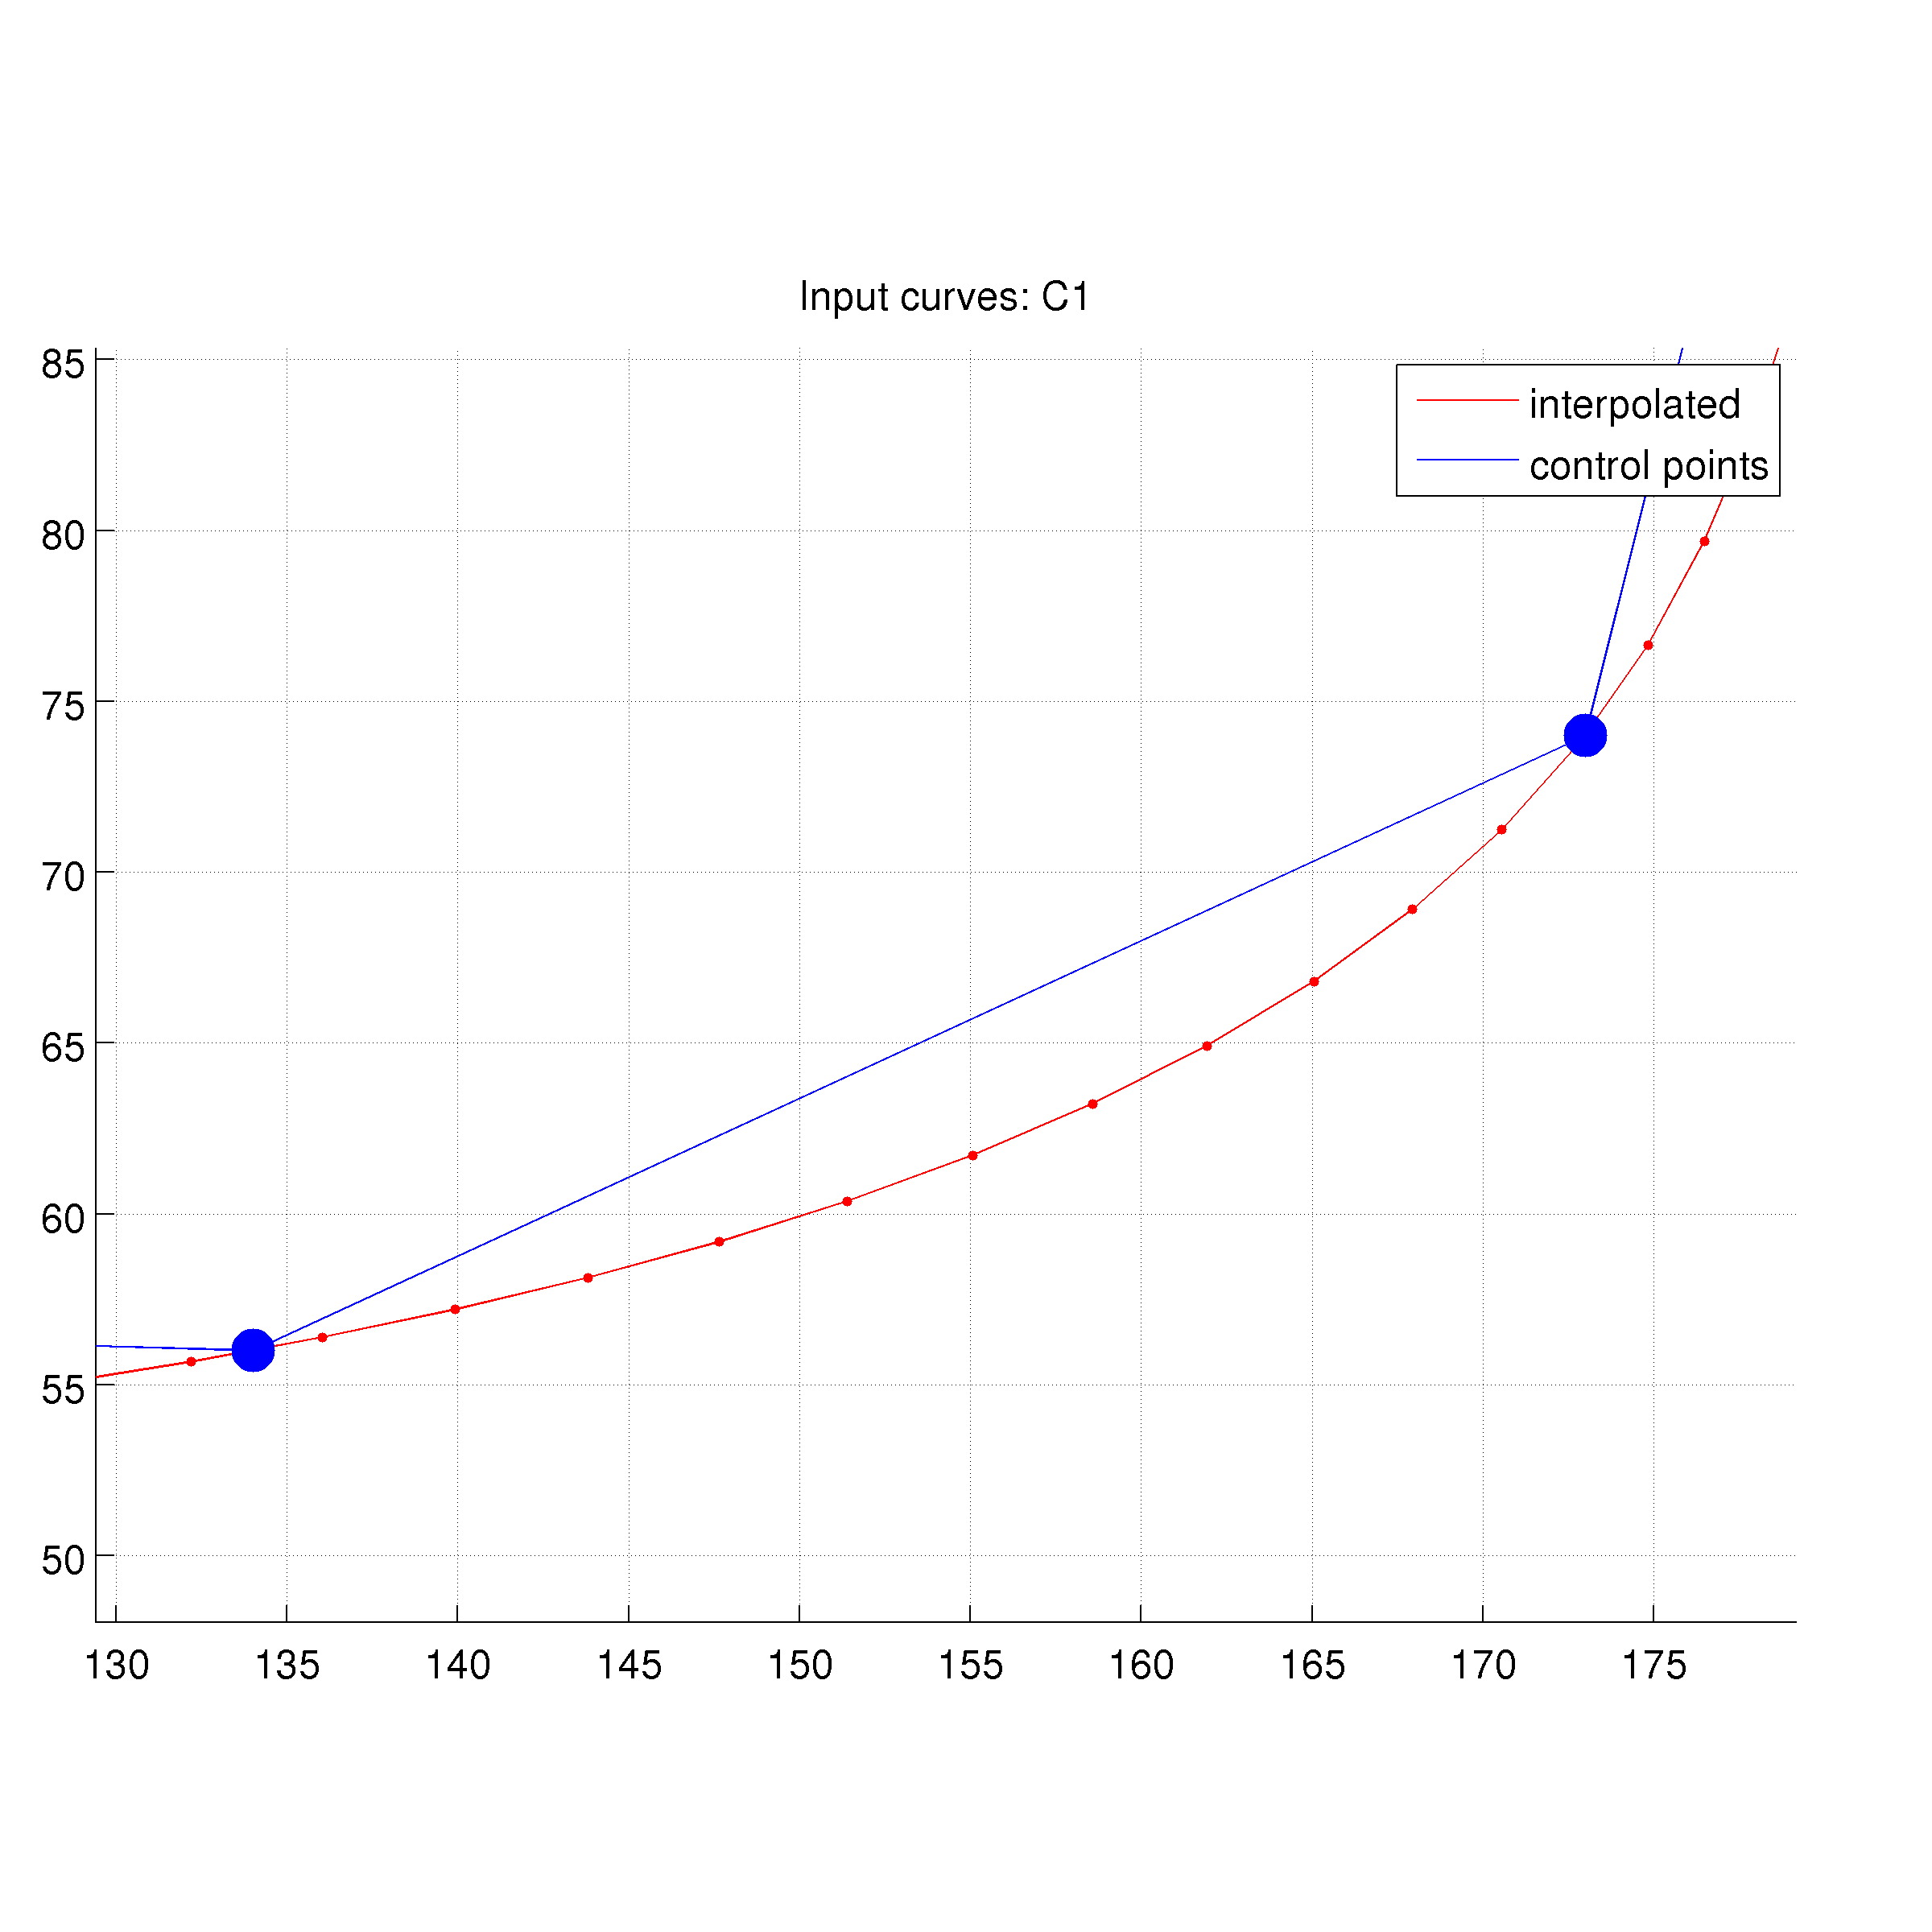
\includegraphics[width=\anchodos]{\chapFiveDir/curves/letter_u/c1_detail}
		\label{fig:curve_interpolation:control_points:detail}
	}
	\caption{Example of preprocessing of an input curve given by control points. 
		\protect\subref{fig:curve_interpolation:control_points:c1} Complete curve with sparse control points are represented in blue and interpolated points are shown in blue.
		\protect\subref{fig:curve_interpolation:control_points:detail} Detail of the lower right part of the curve.
	}
	\label{fig:curve_interpolation:control_points}
\end{figure}

The morphing technique we will propose in Chapter \ref{chap:image_interpolation} works with sparsely sampled curves (polylines), which are used as control points of the warping algorithm. In order to develop a curve interpolation algorithm usable in this case, we must obtain a dense representation of the curve. In this section we explain such interpolation under the (strong) assumption that the interpolation method used to generate  the curve between those control points can be arbitrarily chosen. This is a big hypothesis, which has to be validated for our application and test if it introduces noticeable alterations in the interpolation results.

Given a set of control points $CP=\left\{(x_k,y_k) \: , \: k \in [0 \ldots K-1]\right\}$, we consider them as a sampling of an unknown function $C(t)=(x(t),y(t))$, with an irregular sampling step $\Delta t_k$. In order to increase the sampling rate, we can approximate the length of the curve by $L=\sum_{k=0}^{K-1} \Delta k$ and specify the desired number of samples $M$ of the newly generated curve. Thus, the new sampling step is determined as $dt=L/M$ and the new sampled parameter $t_m$ is generated. Using this parameter we perform the interpolation by
using piecewise cubic spline interpolation to generate a dense curve between the control points. We look at each coordinate of $C(t)$ as a one dimensional function $\mathcal{R}\rightarrow\mathcal{R}$ and interpolate each one independently. Thus the interpolated samples $(x_m,y_m)$ are computed as
\begin{equation}
\begin{array}{l}
 (x_m,y_m)=\mathcal{I}((x_k,y_k),t_k,t_m) \\
 \mbox{with} \: k=0,\ldots,K-1 \: \mbox{and} \: m=0,\ldots,M-1
 \end{array}
\end{equation}
where  $\mathcal{I}$  is the interpolating function used.\\
With the interpolation scheme presented above, we compute all the differential magnitudes and the curvature signatures as before. In Figure \ref{fig:image_interpolation:curve_interpolation:polyline:normals} we show the approximation of the differential magnitudes. As it happened in the dense case, the obtained parametrization is very close to arc-length, with velocities very close to unit. These minor deviations (Fig. \ref{fig:image_interpolation:curve_interpolation:polyline:normals:mod_vel}, red curve) from unit speed are caused by insufficient sampling in high curvature parts of the curve. In this example, this happens near the \emph{corners} of the U letter. In addition, the first peak is higher because the left corner of the letter has a narrower turn than the right one.
This can be alleviated by increasing the uniform sampling rate used (Fig. \ref{fig:image_interpolation:curve_interpolation:polyline:normals:mod_vel}, blue curve) or by using an adaptive sampling algorithm based on curvature. In  \cite{geometry:curves:surazhsky:2004:sampling_planar_curves} correct sampling of planar curves is discussed in depth and adaptive sampling algorithms are proposed.

\begin{figure}[h]
	\centering
	\subfloat[]{
		\raisebox{-0.12\height}{\includegraphics[width=\anchodos]{\chapFiveDir/curves/letter_u/curve_curvature_spatial_edited}}
		\label{fig:image_interpolation:curve_interpolation:polyline:normals:curvature_spatial}
	}\\
		\subfloat[]{
		\includegraphics[width=\anchodos]{\chapFiveDir/curves/letter_u/curve_curvature_edited}
		\label{fig:image_interpolation:curve_interpolation:polyline:normals:curvature}
	}
	\subfloat[]{
		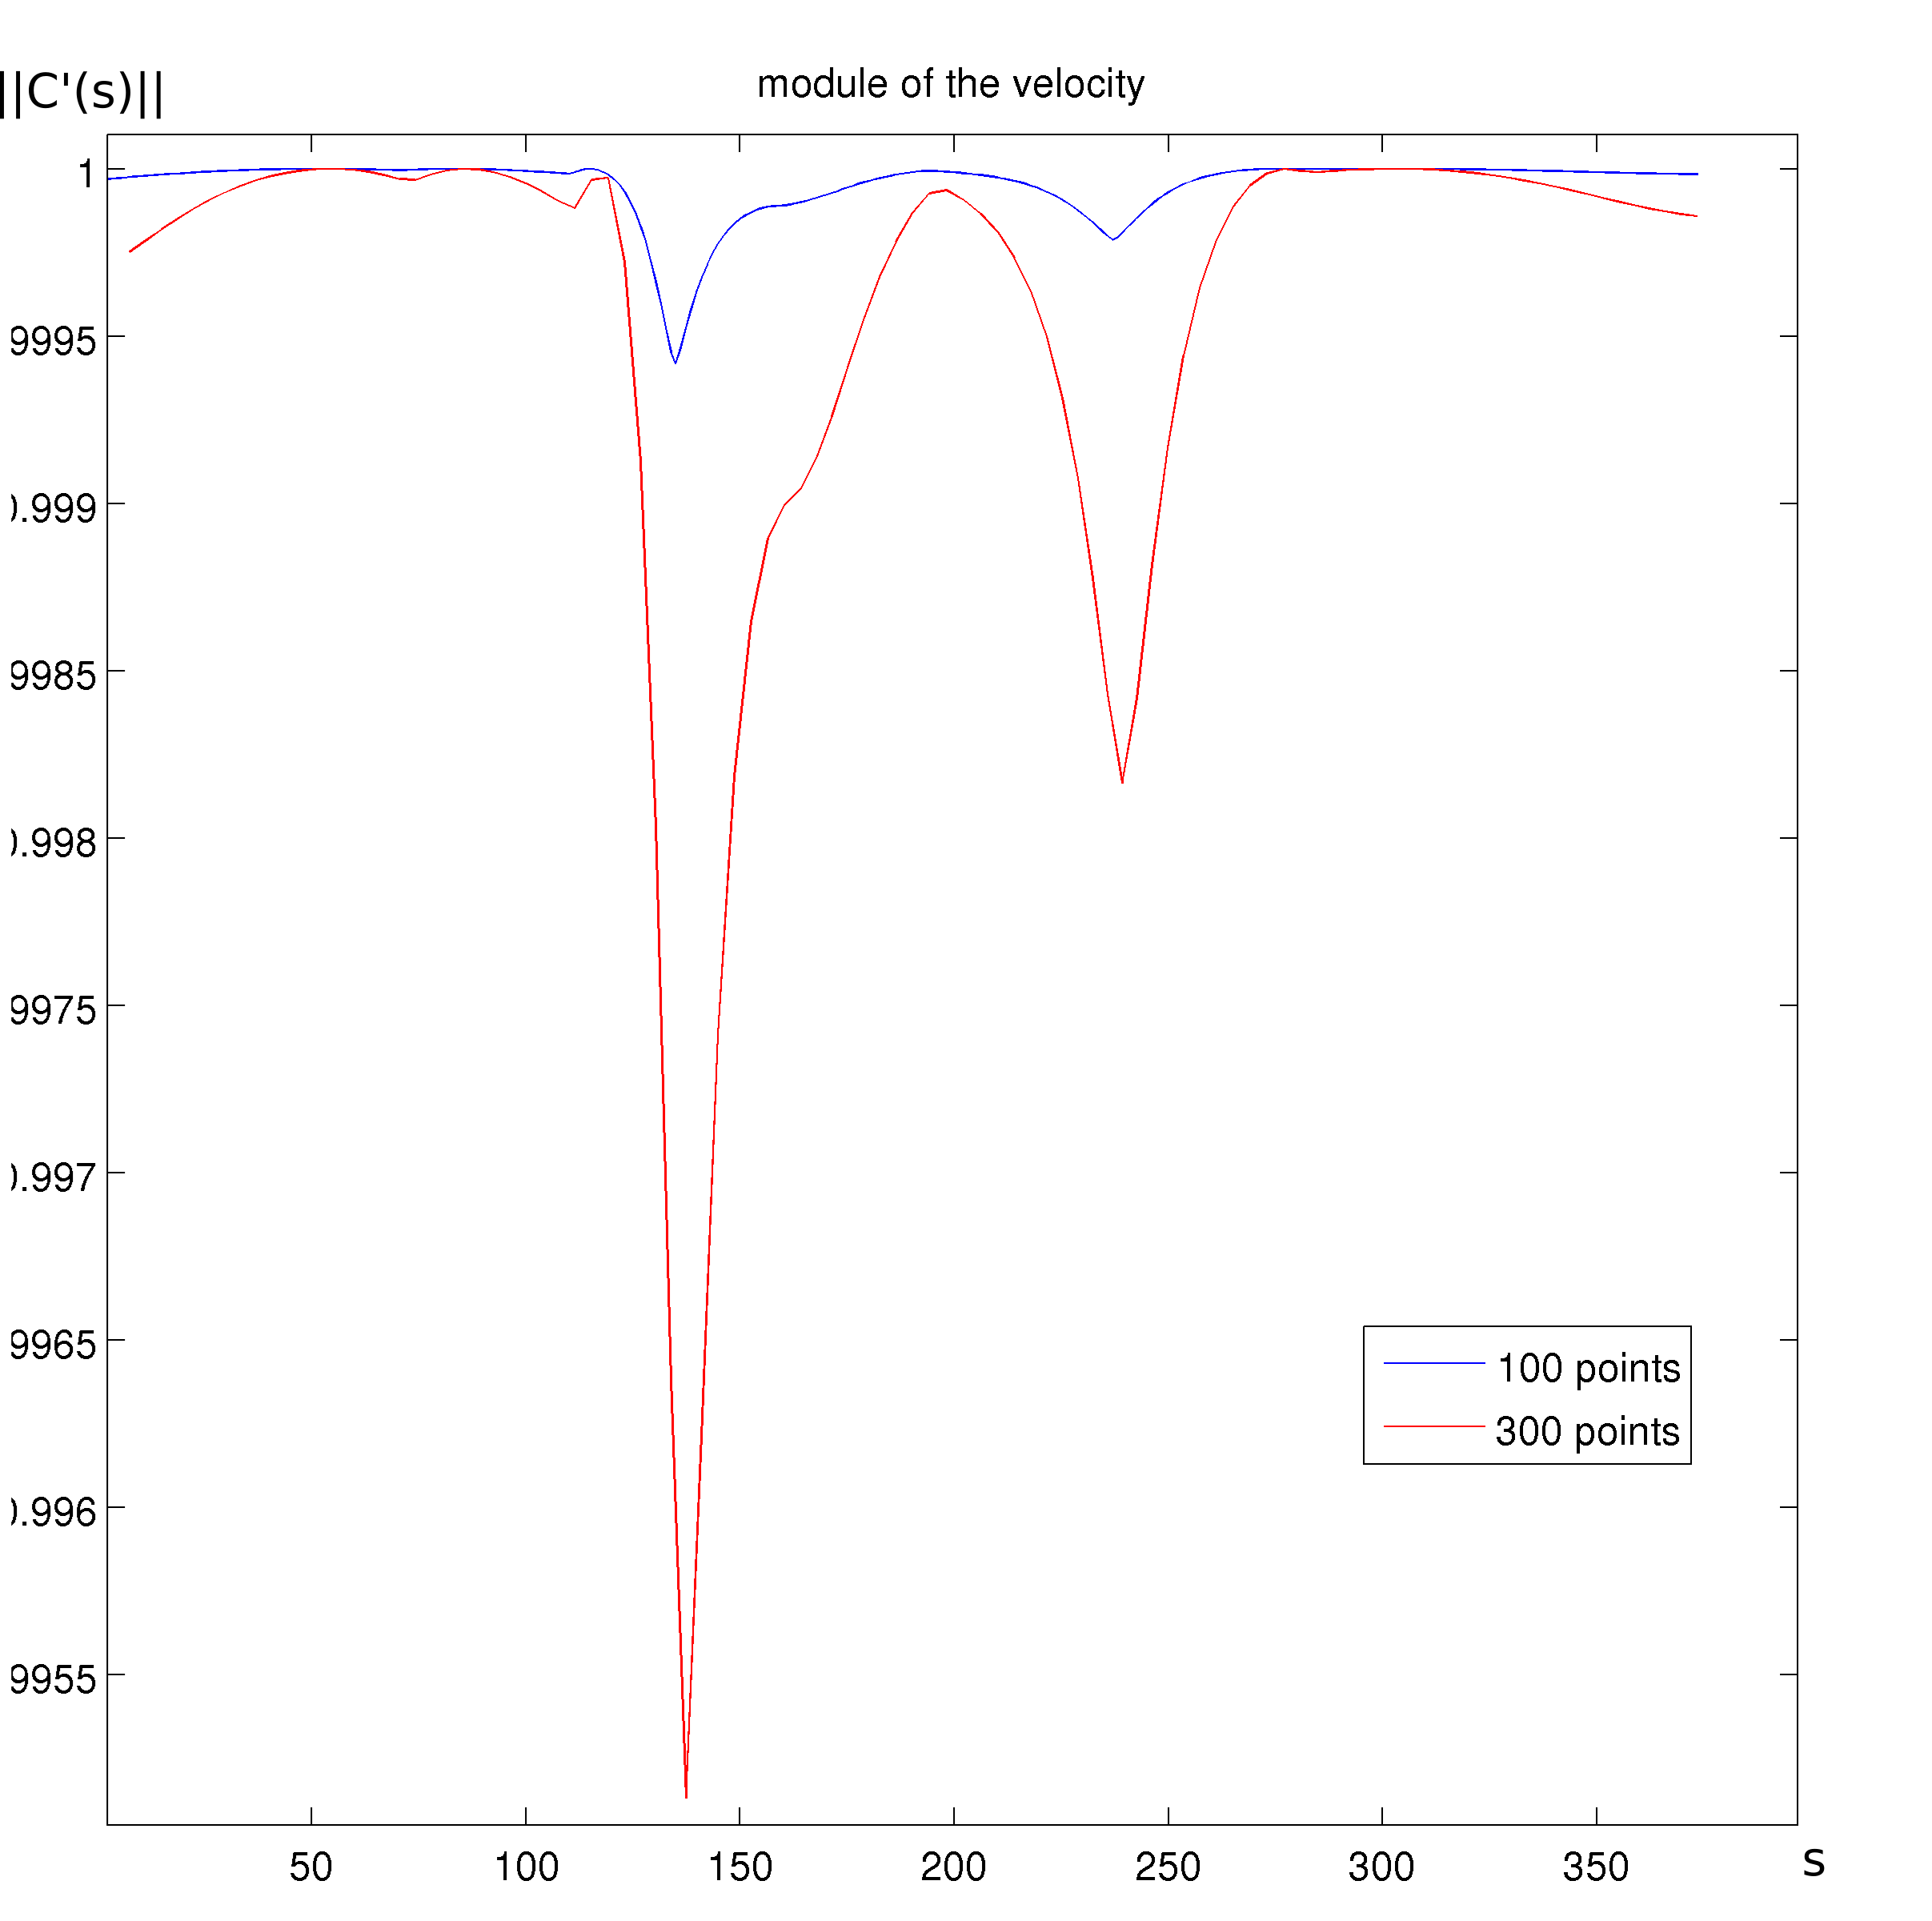
\includegraphics[width=\anchodos]{\chapFiveDir/curves/letter_u/curve_mod_vel_comparison_edited}
		\label{fig:image_interpolation:curve_interpolation:polyline:normals:mod_vel}
	}
	\caption{Computation of curvature signatures in the case of a curve interpolated from sparse control points. The curve corresponds to a hand written U letter. \protect\subref{fig:image_interpolation:curve_interpolation:polyline:normals:curvature_spatial} Original polyline, its dense approximation using cubic splines and the curvature plotted as the vector $C''(s)=\kappa(s)N(s)$. \protect\subref{fig:image_interpolation:curve_interpolation:polyline:normals:curvature} Curvature signature, its peaks correspond to the higher curvatures zones near the \emph{corners} of the letter.
		\protect\subref{fig:image_interpolation:curve_interpolation:polyline:normals:mod_vel} Module of the tanget vector field using 100 and 500 points to interpolate between each pair of control points.
		Please note that the curvature peaks occur at parameter values of 137 and 239, same as the peaks in the module of the velocity.
}
	\label{fig:image_interpolation:curve_interpolation:polyline:normals}
\end{figure}

\subsection{Reconstruction from curvature signatures}
In previous sections we presented a way to describe intrinsic curve properties using curvature signatures and how to compute them in our two cases of interest: dense and sparsely sampled curves.
Once we have this transform, we can perform shape operations intuitively in this space. After these operations are performed, we will need a way to invert the transform and recover the curve.
Under the point of view of a transform, we will call Euclidean to the original space where the curve is expressed in 2D coordinates and curvature or transform space to the destination space, where curves are represented by curvature signatures.
We will call transform to the computation of the curvature signature and antitransform or reconstruction to the inverse process.

The inverse problem (reconstruct) is far more difficult that the forward one (transform), because the transform process involves computing derivatives and to achieve the opposite we will need to integrate those derivatives. We must bear in mind that in the transform process we lost the extrinsic parameters of the curve (rotation and translation), so we will have these two degrees of freedom once we reconstruct the curve.

Let us recall that $C'(s)=T(s)$ and $C''(s)=T'(s)=\kappa(s)N(s)$. As we are assuming arc-length parametrization, $T(s)=(x'(s),y'(s))$ is a unit norm vector which is always on the unit circle. Thus we can describe it by means of $\theta$,  its angle with respect to the $x$-axis , which is expressed as
\begin{equation}
 \theta(s)=\tan^{-1}\left(\frac{y'(s)}{x'(s)}\right).
 \label{eq:image_interpolation:curve_interpolation:theta}
\end{equation}

If we compute $\theta'(s)$ using the expression given in Equation \ref{eq:image_interpolation:curve_interpolation:theta}, we obtain

\begin{equation}
 \theta'(s)=x'(s)y''(s)-x''(s)y'(s) ,
 \label{eq:image_interpolation:curve_interpolation:theta_prime}
\end{equation}

which is exactly the same expression we obtained for $\kappa(s)$ in Equation \ref{eq:image_interpolation:curve_interpolation:curvature_reparametrized}. Thus $k(s)=\theta'(s)$, and if $k(s)$ is known, we can recover $\theta(s)$ up to an initial condition $\theta(0)=\varphi_0$. This initial angle corresponds to the missing global rotation of the curve which was lost in the transform process, so this reduces one of the degress of freedom. Thus, the reconstructed angle can be expressed as

\begin{equation}
 \theta(s)=\int_0^s k(\tilde{s})d\tilde{s}+\varphi_0
  \label{eq:image_interpolation:curve_interpolation:angle_reconstruction_from_curvature}
\end{equation}

The function $\theta(s)$, can be also regarded as a curve signature or transform, in the sense that it also describes the shape curve in an \emph{almost} complete way. But both $\kappa(s)$ and $\theta(s)$ are scalar magnitudes, and $C(s)=(x(s),y(s))$ is a vector-valued function, so we need a way to construct $C(s)$ from $\theta(s)$. If we recall that $T(s)$ is a vector lying on the unit circle and $\theta(s)$ its angle with the $x$-axis, we can express $T(s)$ in terms of $\theta(s)$. Let $Circ(s)$, with $s\in[0,2\pi)$, be an arc-length representation of the unit circle, which can be expressed as $Circ(s)=(cos(s),sin(s))$. Then, we can express the tangent field as $T(s)=Circ(\theta(s))$ and we can compute it as
\begin{equation}
T(s)=Circ \left(\int_0^s k(\tilde{s})d\tilde{s}+\varphi_0 \right).
 \label{eq:image_interpolation:curve_interpolation:tangent_reconstruction}
\end{equation}

Finally, in order to reconstruct $C(s)$ we need to integrate again and add another initial condition, which will be the missing translation $x_0$. Thus 

\begin{equation}
C(s)=\int_0^s T(\bar{s} ) d\bar{s} +x_0
 \label{eq:image_interpolation:curve_interpolation:curve_reconstruction}
\end{equation}

or equivalently

\begin{equation}
C(s)=\int_0^s Circ(\theta(\bar{s}) ) d\bar{s} +x_0 .
\label{eq:image_interpolation:curve_interpolation:curve_reconstruction_from_angle}
\end{equation}

If we expand Equation \ref{eq:image_interpolation:curve_interpolation:curve_reconstruction}, the complete computation becomes

\begin{equation}
C(s)=\int_0^s Circ\left(\int_0^{\bar{s}}  k(\tilde{s})d\tilde{s}+\varphi_0 \right) d\bar{s}  +x_0
\label{eq:image_interpolation:curve_interpolation:curve_reconstruction_complete}
\end{equation}


In the original paper the authors propose to approximate the non-linear $Circ(s)$ function by means of rational functions, which allows them to carry the computations of the reconstruction analytically. As we are only interested in using this technique to interpolate control curves, we have chosen to solve the inverse problem numerically. We carry this computation in two steps:
\begin{enumerate}
	\item First, integrate the curvature $\kappa(s)$ to obtain the angle $\theta(s)$ according to Equation  \req{eq:image_interpolation:curve_interpolation:angle_reconstruction_from_curvature}.
	\item Then, integrate the recovered angle $\theta(s)$ to obtain the curve $C(s)$ according to Equation \req{eq:image_interpolation:curve_interpolation:curve_reconstruction_from_angle}.
\end{enumerate} 
Note that the numerical errors of the first step are passed to the input of the second step, thus the integration of the first step is performed using a higher order numerical scheme. In this case we used an explicit fourth order Runge-Kutta scheme \cite{math:numerical:dormand:1980:a_family_of_embedded_runge_kutta}. For the second step we use a standard trapezoid rule.
Finally, as the integral is carried out using an explicit scheme, errors tend to accumulate and will produce greater differences for  big $s$ value. In Figure~\ref{fig:image_interpolation:curve_interpolation:reconstruction:sine:initial:curvature_50} we show the results of such approach. As expected, the error grows bigger as we move through the curve in the increasing $s$ direction. 
Despite the error, which could be easily avoided using an implicit scheme, this demonstrates that the reconstruction works as expected. In addition, in Figure \ref{fig:image_interpolation:curve_interpolation:reconstruction:sine:initial:curvature_phi_0} we show the reconstruction using a different initial condition for the angle $\varphi_0$, and we observe that the shape is still correctly recovered but the global orientation is incorrect.

\begin{figure}[h]
	\centering
	\subfloat[]{
		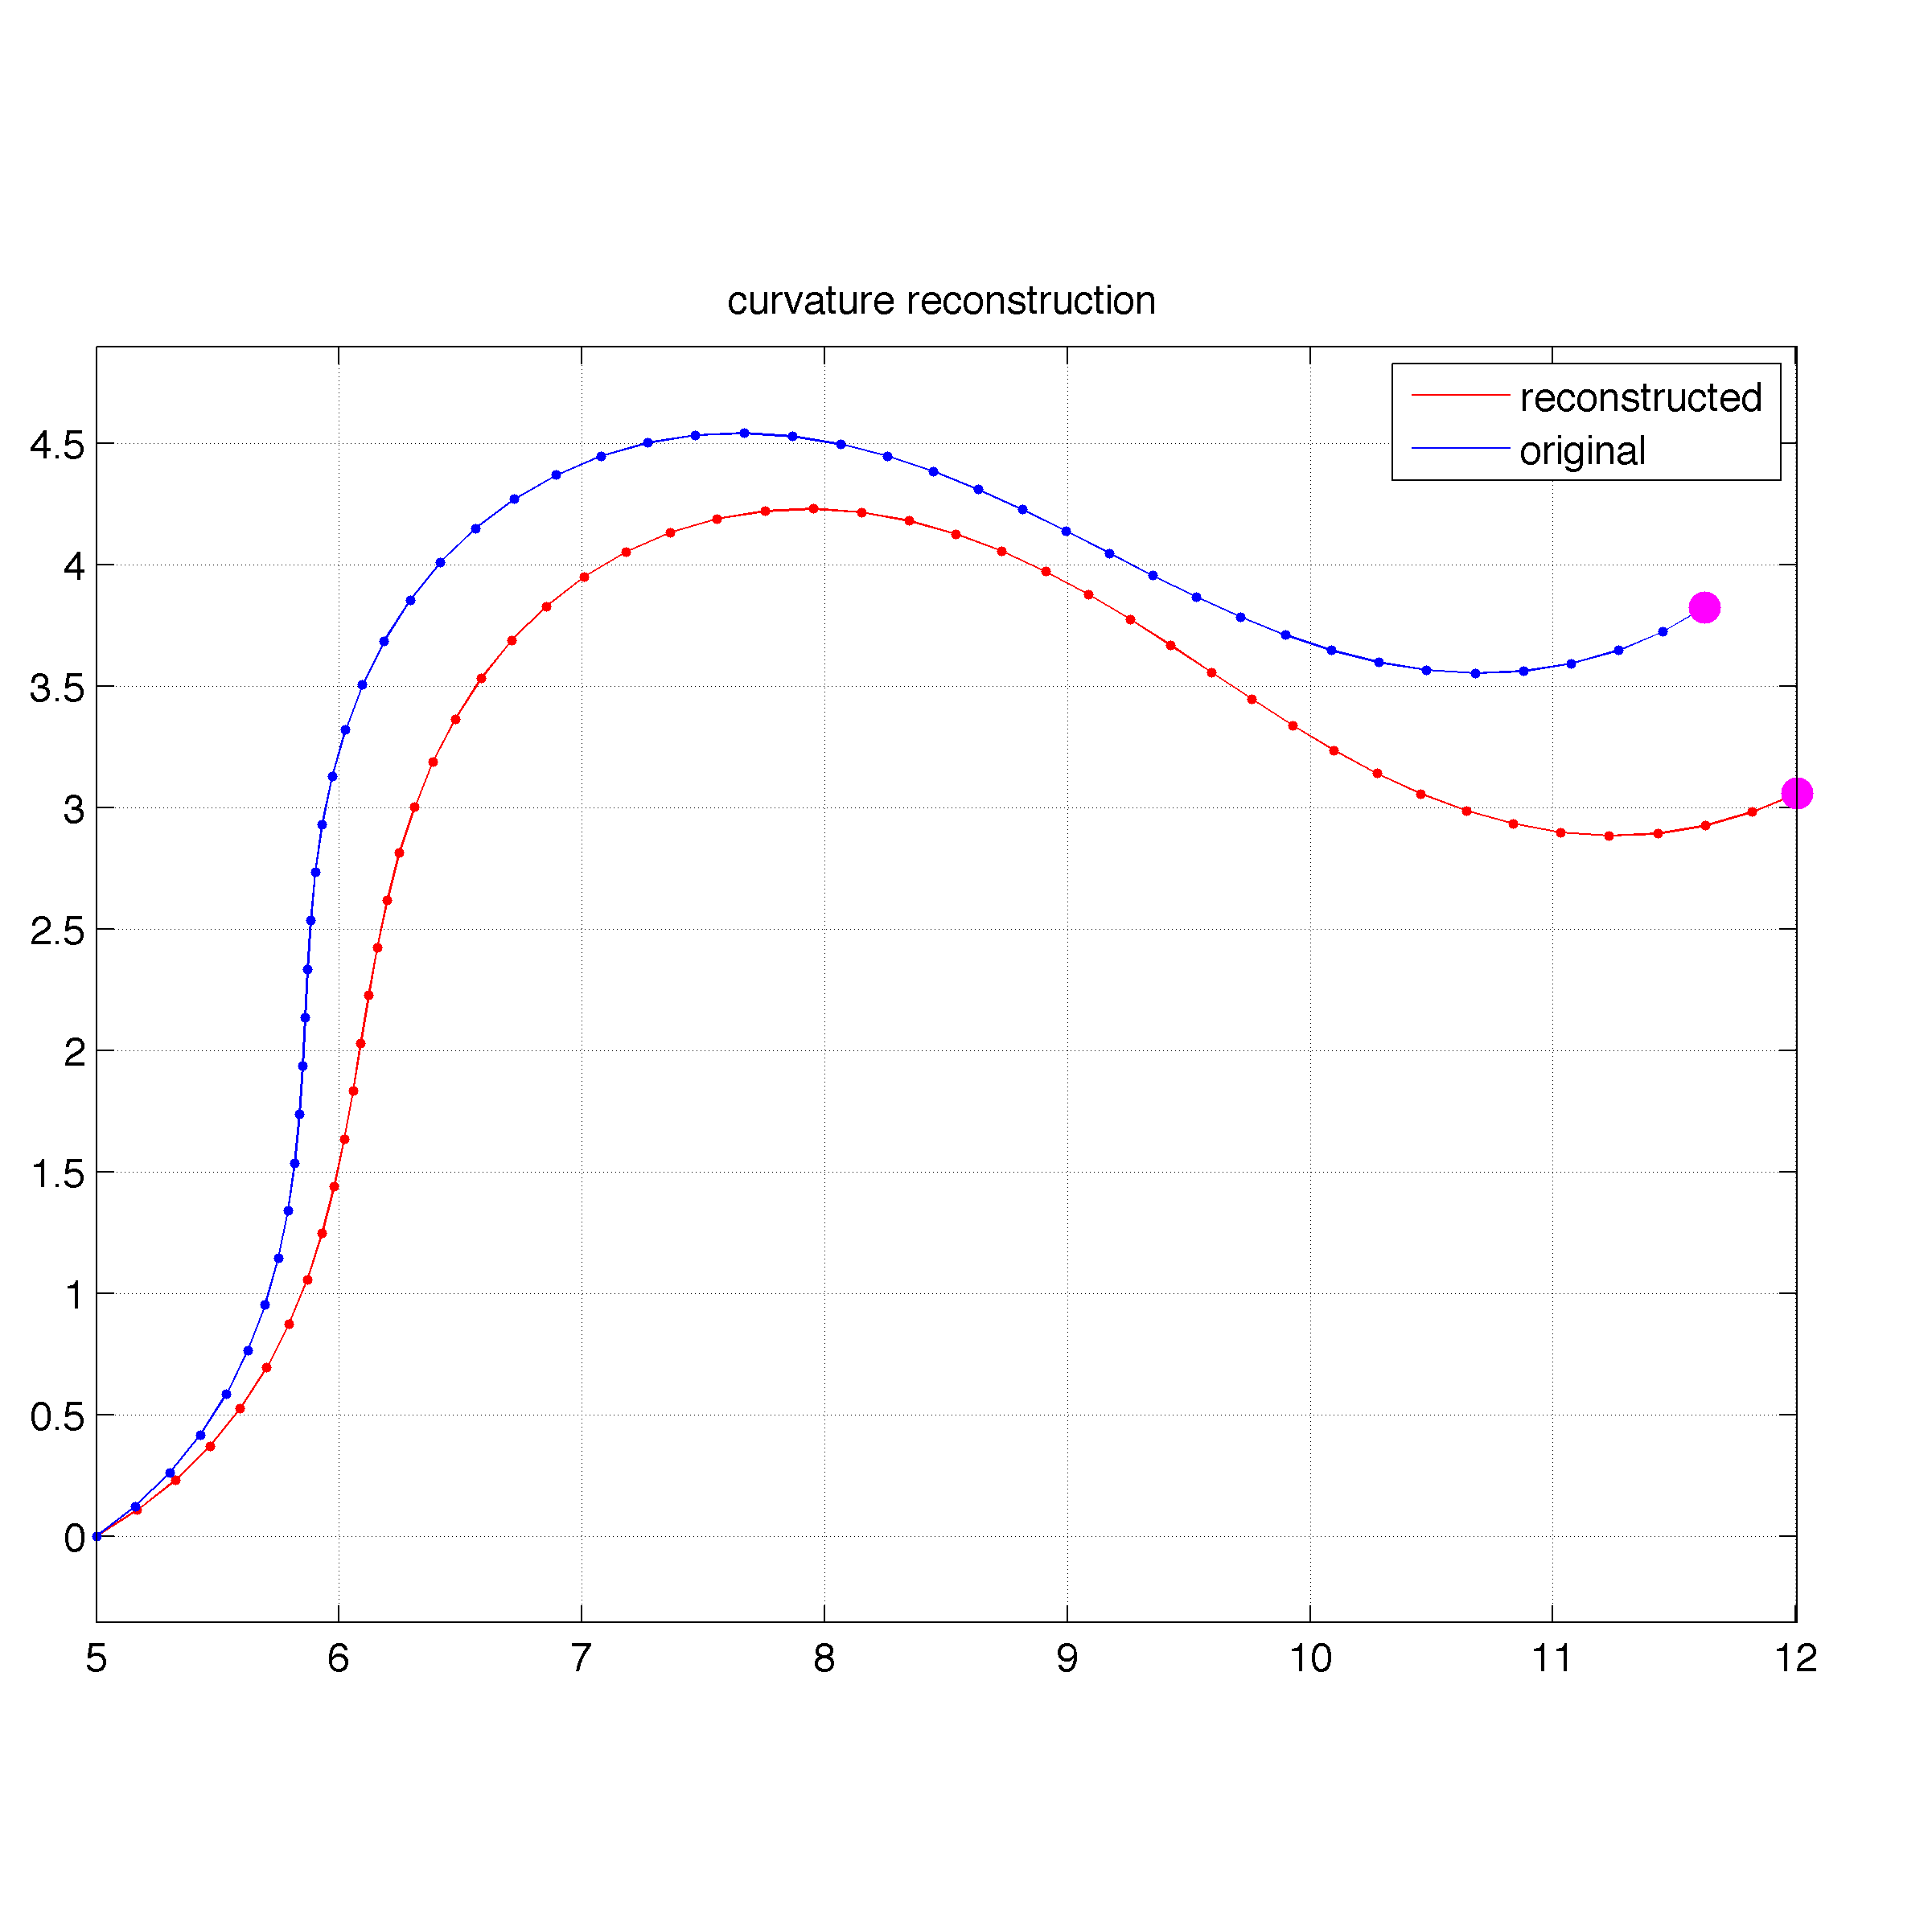
\includegraphics[width=\anchodos]{\chapFiveDir/curves/sine/curve_reconstructed_curvature_50}
		\label{fig:image_interpolation:curve_interpolation:reconstruction:sine:initial:curvature_50}
	}
	\subfloat[]{
		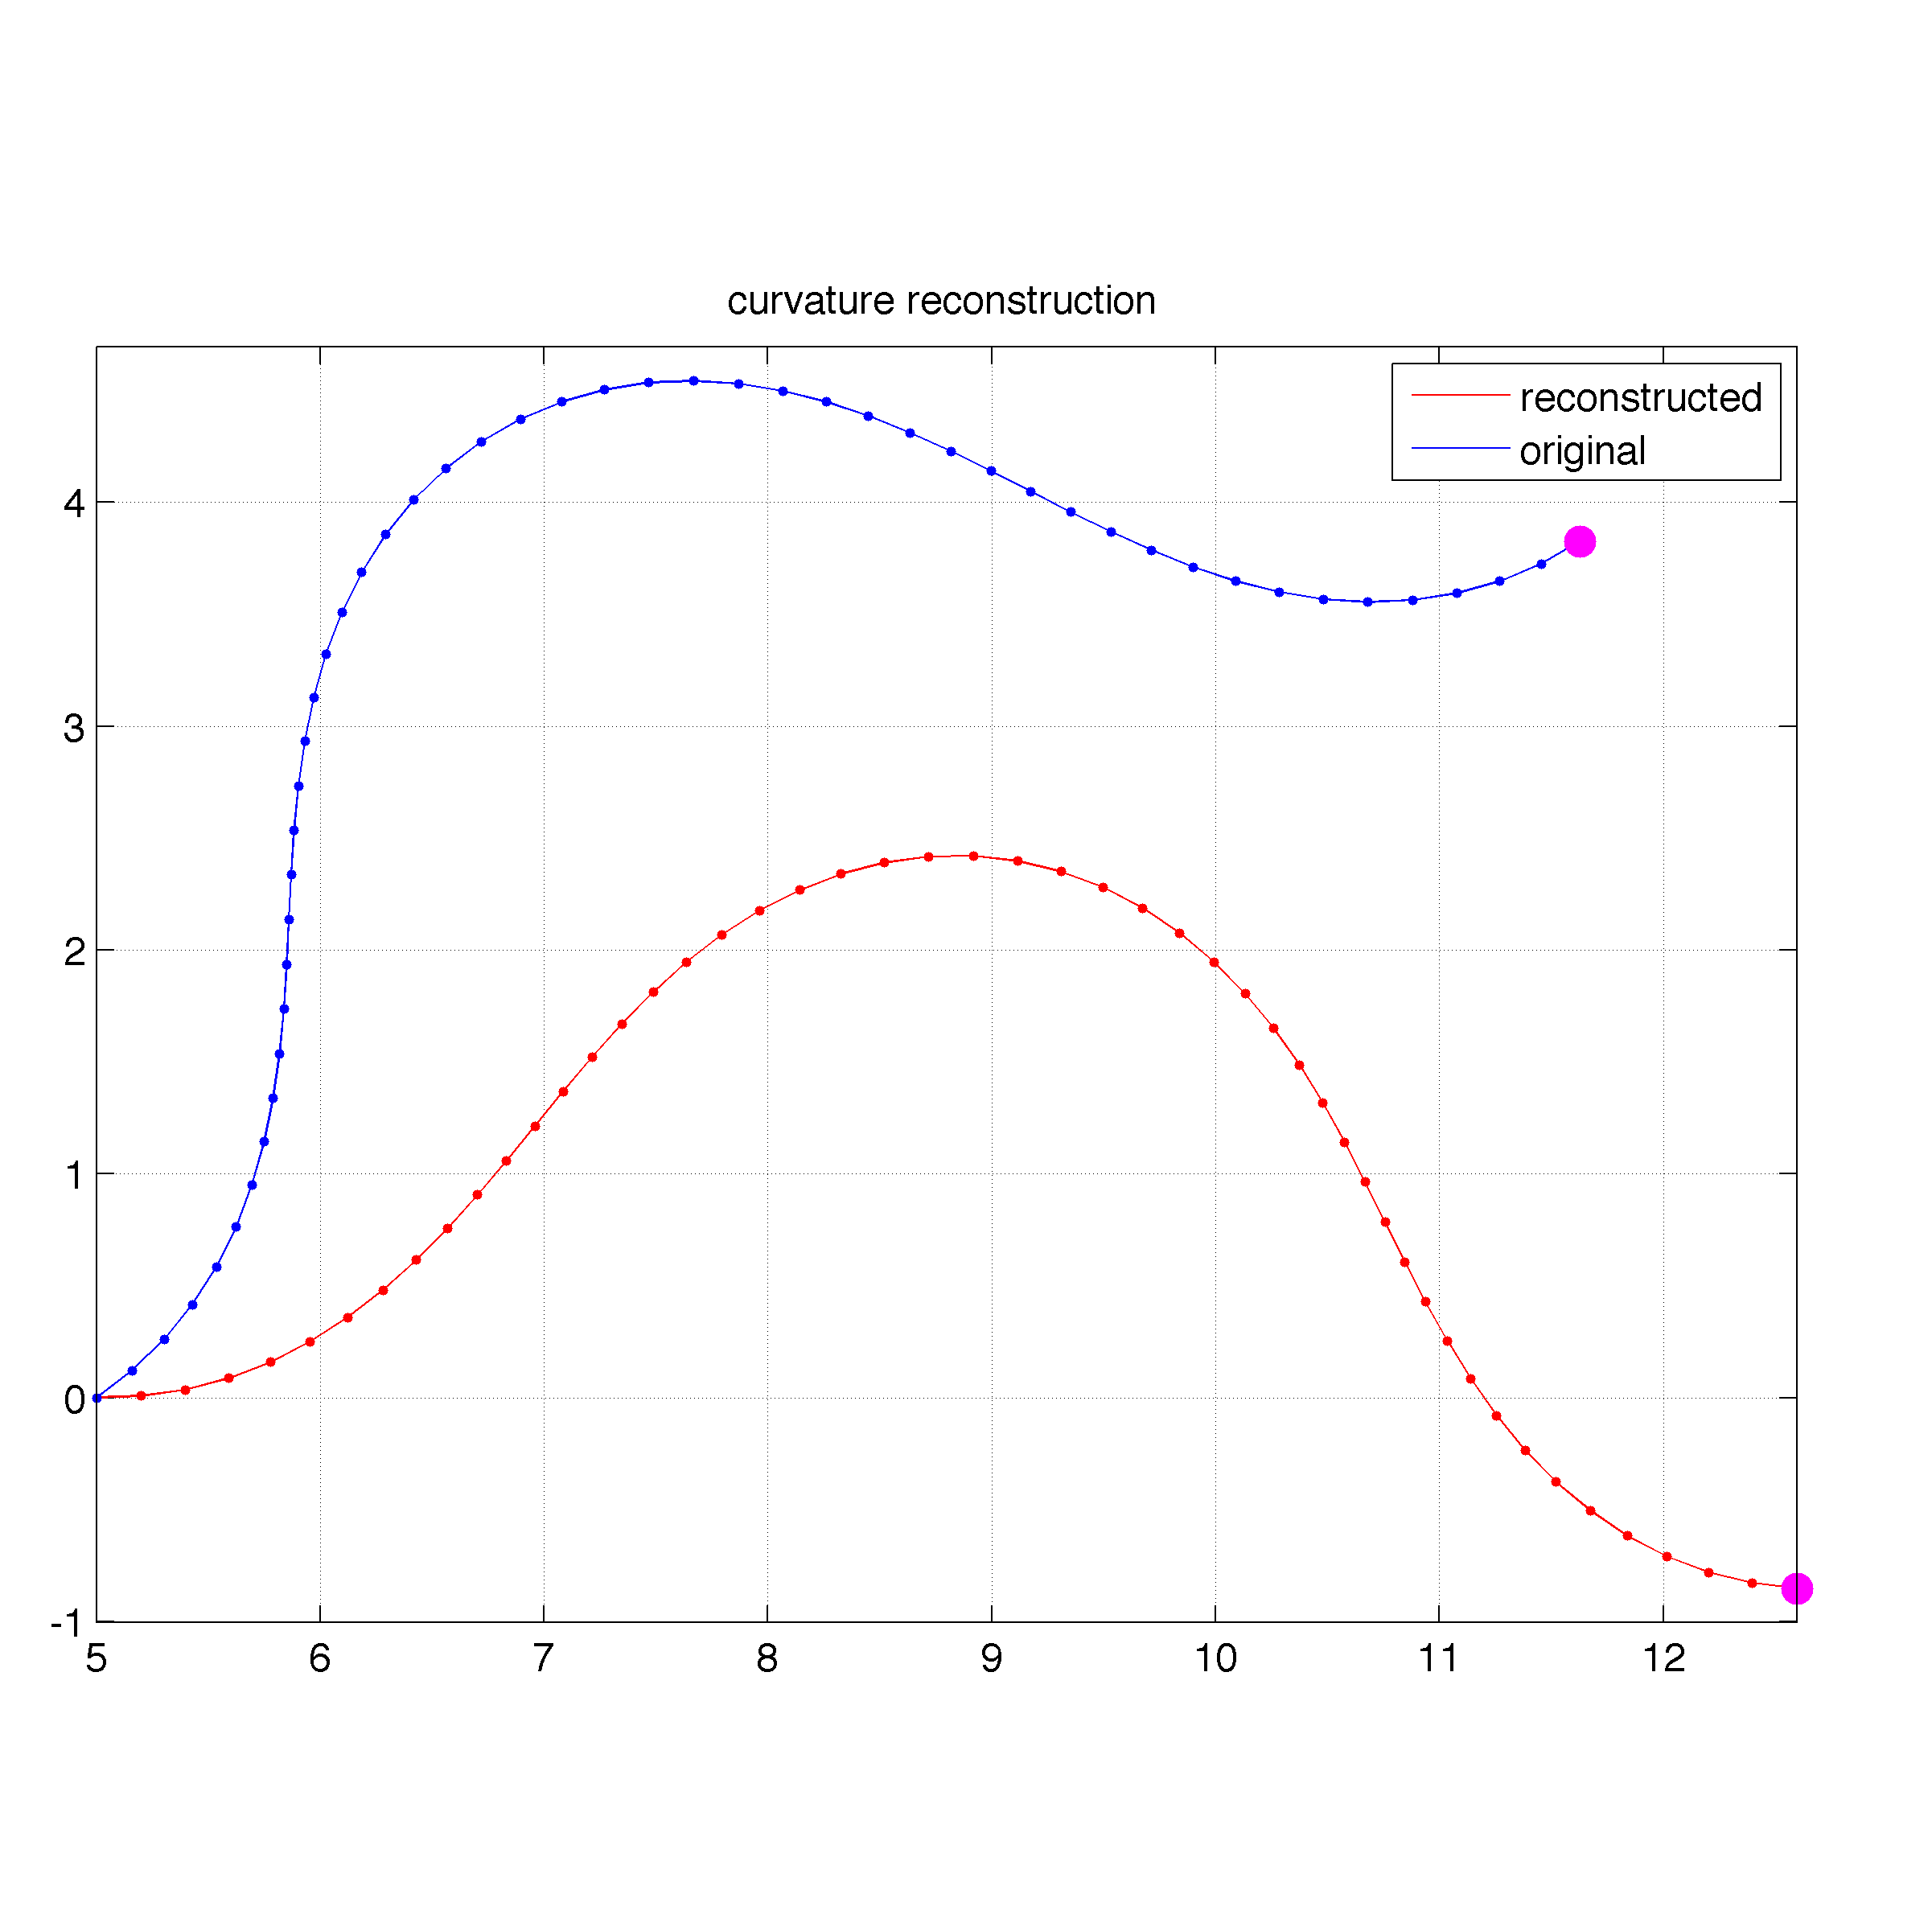
\includegraphics[width=\anchodos]{\chapFiveDir/curves/sine/curve_reconstructed_curvature_phi_0}
		\label{fig:image_interpolation:curve_interpolation:reconstruction:sine:initial:curvature_phi_0}
	}
	
	\caption{Reconstruction of a curve from its curvature signature. We transform an original curve sampled at 50 points and then reconstruct the original curve from the transformed one. The magenta dots show the points where the reconstruction error is maximum.
		\protect\subref{fig:image_interpolation:curve_interpolation:reconstruction:sine:initial:curvature_50} Imposing the correct initial angle $\varphi_0=\frac{\pi}{6}$.
		\protect\subref{fig:image_interpolation:curve_interpolation:reconstruction:sine:initial:curvature_phi_0} Imposing a different initial angle $\varphi_0=0$.}
	\label{fig:image_interpolation:curve_interpolation:reconstruction:sine:initial}
\end{figure}

To test the numerical errors, in Figure \ref{fig:image_interpolation:curve_interpolation:reconstruction:sine} we compare different integration approaches. The integration error depends on the sampling step $h$ and the numerical scheme used for each step. We compute this error as the average L2-difference of the reconstructed curve  with the original one, relative to the magnitude of the original curve.
\begin{equation}
 \epsilon=\frac{1}{N}\sum_i\frac{||C_r(s_i)-C(s_i)||}{||C(s_i)||}, \:\: i\in[1,N]
\end{equation}
where $C(s_i)=(x(s_i),y(s_i))=(x_i,y_i)$ represents the coordinates of the $i$-est point of curve $C$.

As the figure shows, at lower sampling rates, increasing the order of the scheme produces a minor improvement on the error. On the other hand, increasing the sample rate greatly diminishes the reconstruction error.


\begin{figure}[h]
	\centering
		\subfloat[]{
		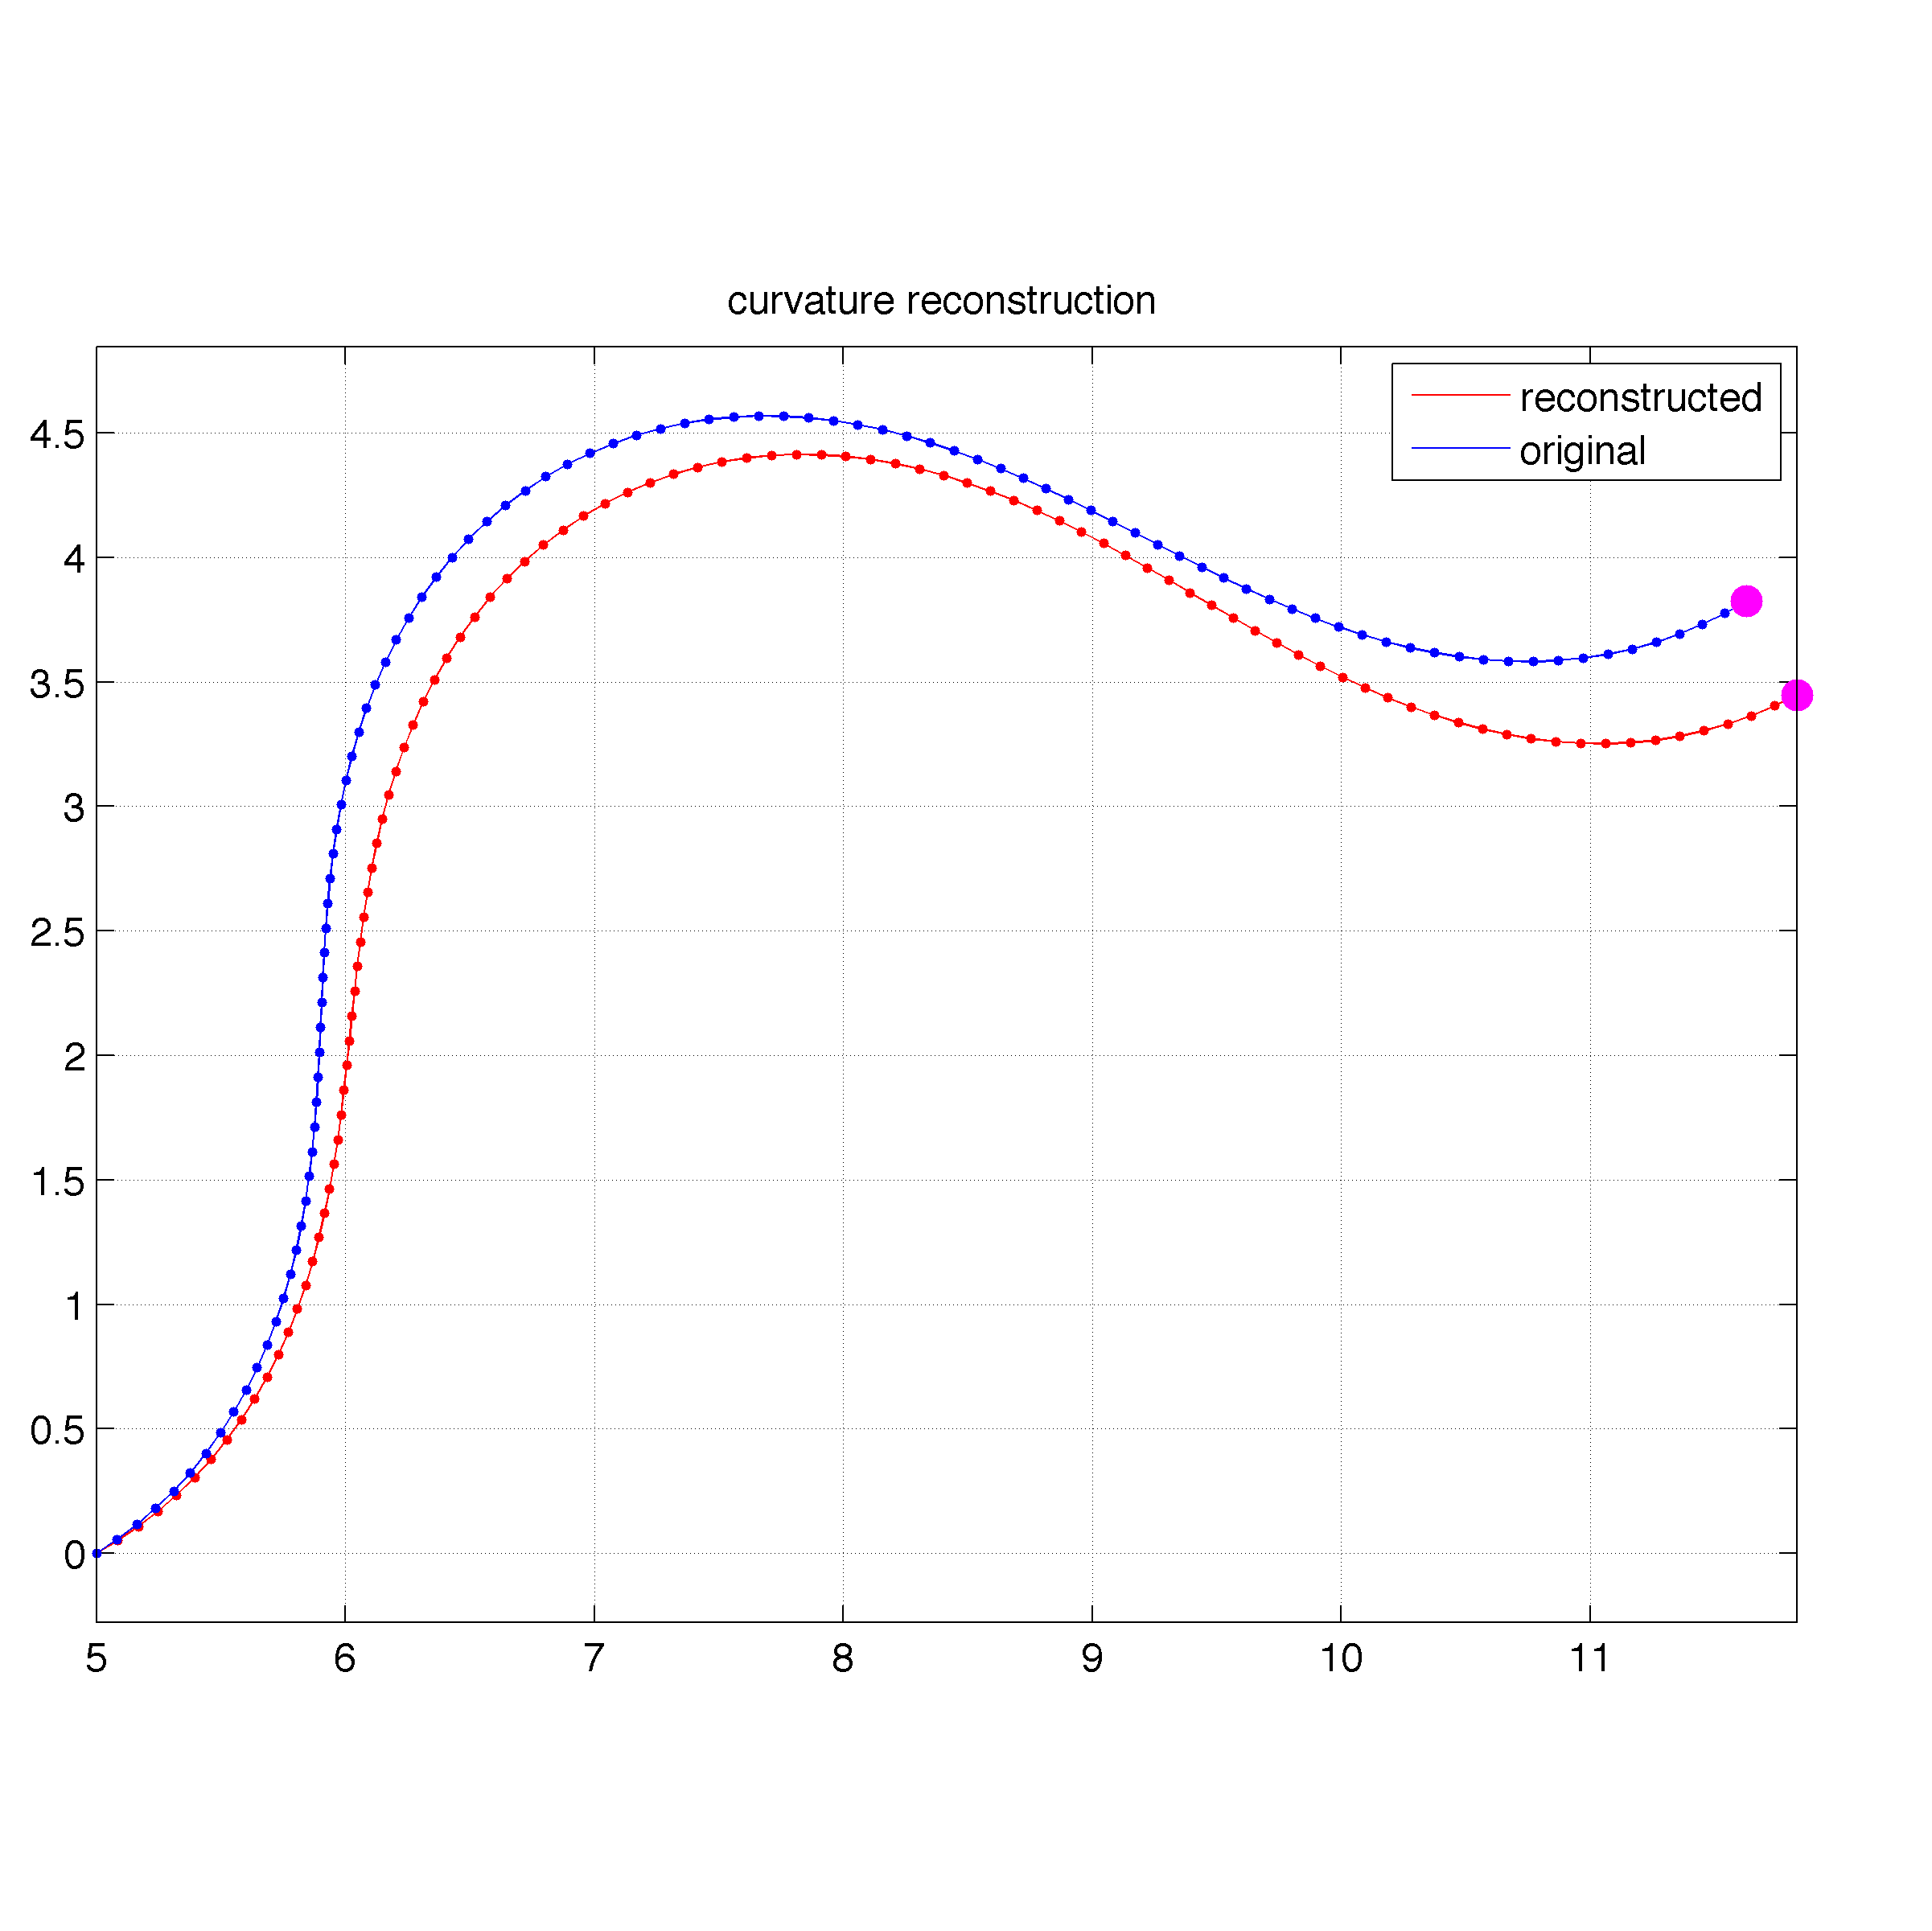
\includegraphics[width=\anchotres]{\chapFiveDir/curves/sine/curve_reconstructed_curvature_100}
		\label{fig:image_interpolation:curve_interpolation:reconstruction:sine:curvature_100}
	}
	\subfloat[]{
		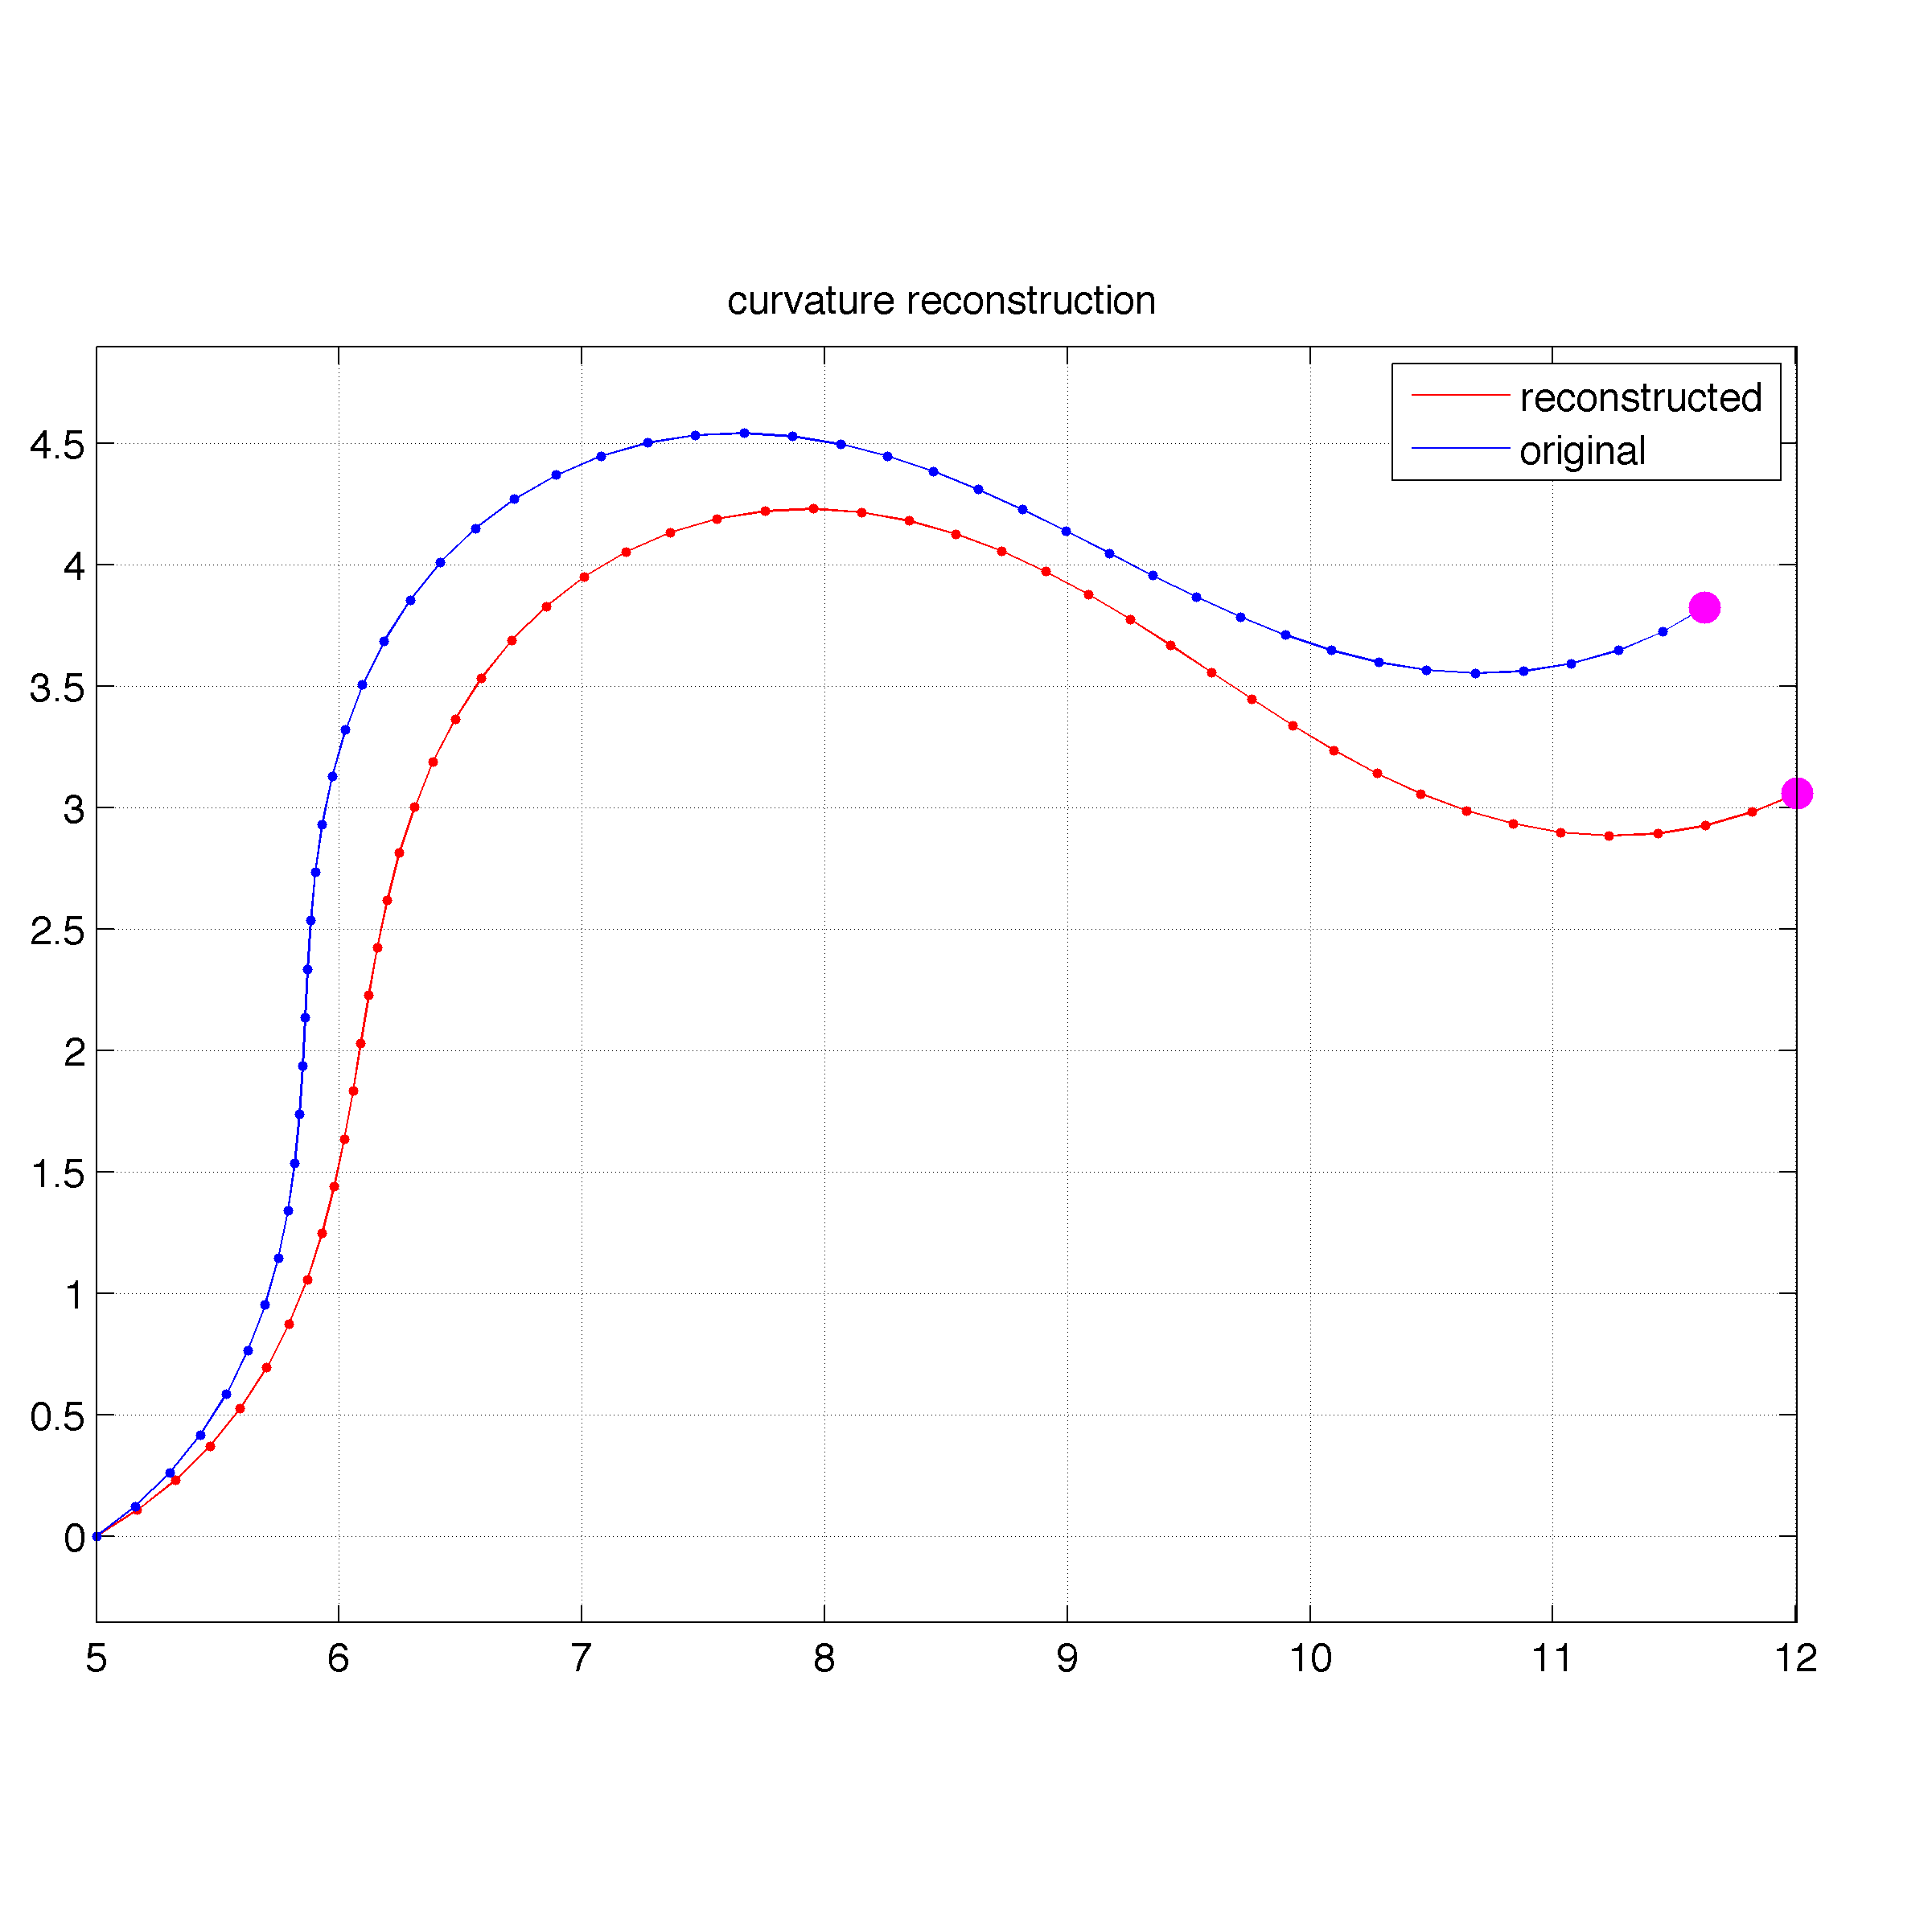
\includegraphics[width=\anchotres]{\chapFiveDir/curves/sine/curve_reconstructed_curvature_50}
		\label{fig:image_interpolation:curve_interpolation:reconstruction:sine:curvature_50}
	}
	\subfloat[]{
		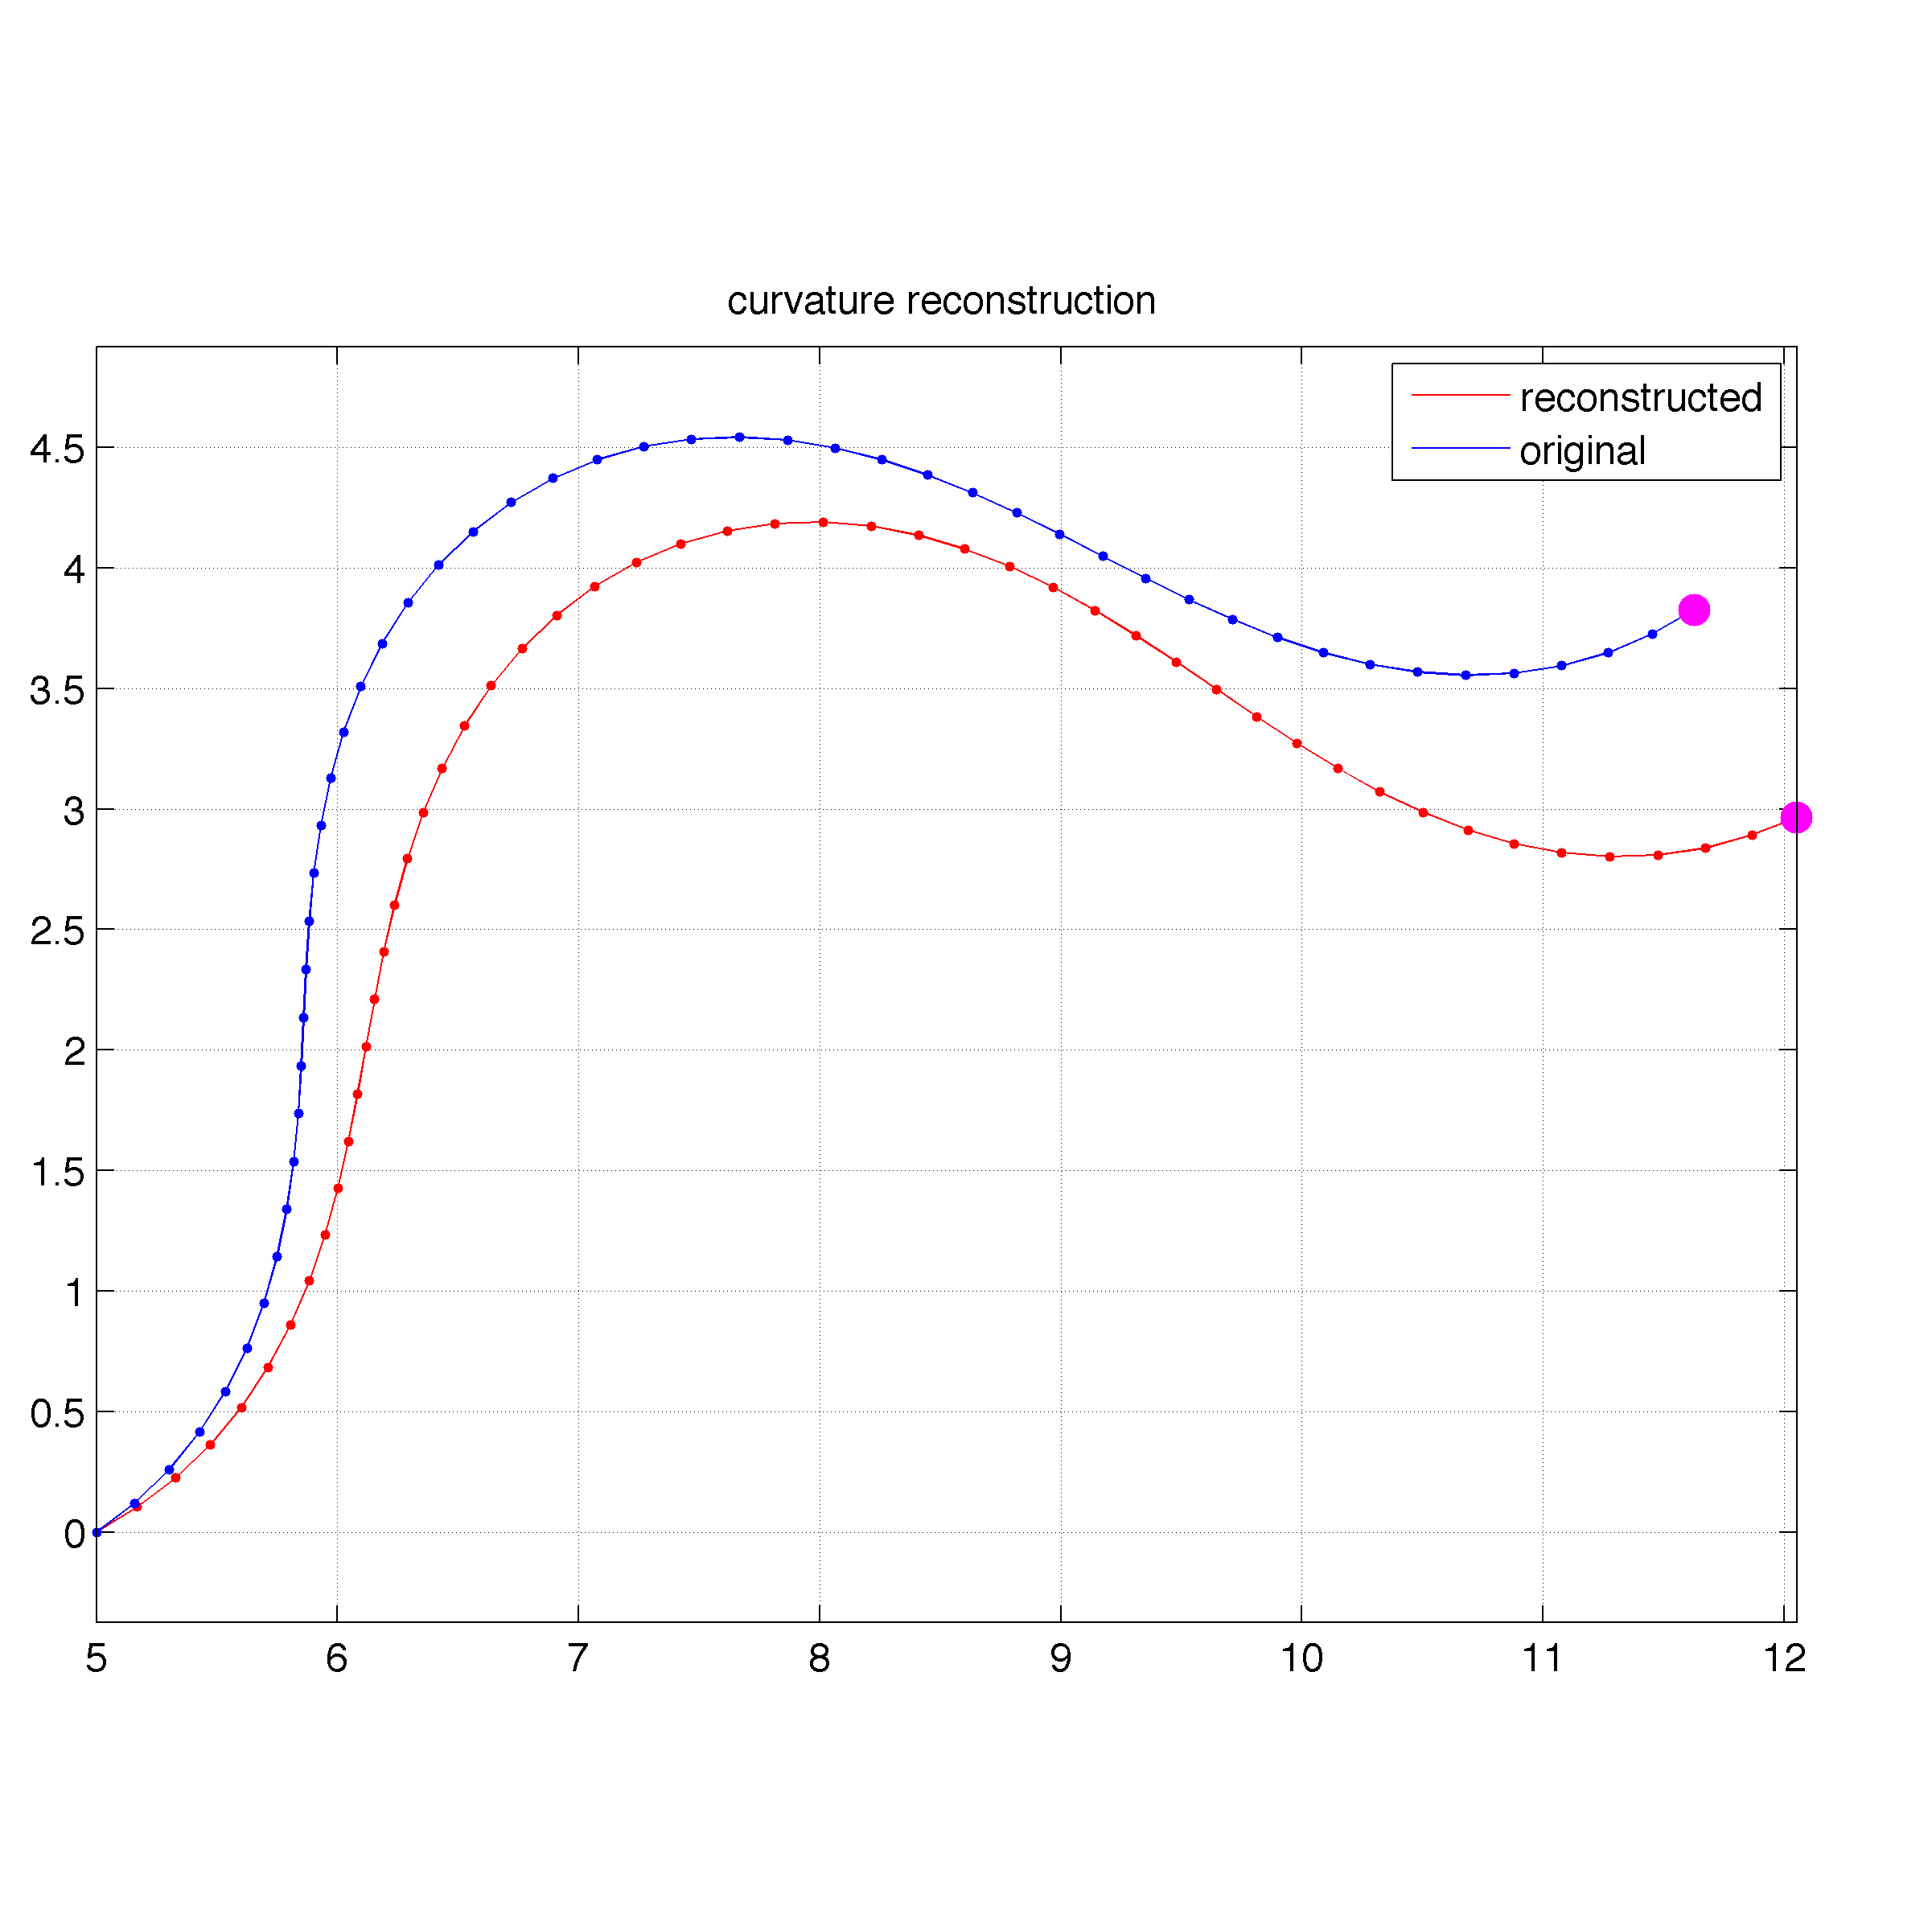
\includegraphics[width=\anchotres]{\chapFiveDir/curves/sine/curve_reconstructed_curvature_lower_50}
		\label{fig:image_interpolation:curve_interpolation:reconstruction:sine:curvature_lower_50}
	}

	\caption{Reconstruction of a curve from its curvature signature. The magenta dots show the points where the reconstruction error is maximum.
				\protect\subref{fig:image_interpolation:curve_interpolation:reconstruction:sine:curvature_100} Original curve sampled at 100 points and the curve reconstructed  from the curvature (Relative error 2.9\%).
				\protect\subref{fig:image_interpolation:curve_interpolation:reconstruction:sine:curvature_50} Original curve sampled at 50 points and the curve reconstructed from the curvature (Relative error 5.9\%).
			\protect\subref{fig:image_interpolation:curve_interpolation:reconstruction:sine:curvature_lower_50} Original curve sampled at 50 points and  the curve reconstructed from the curvature using a lower order numeric method for the first step (Relative error 6.7\%).}
	\label{fig:image_interpolation:curve_interpolation:reconstruction:sine}
\end{figure}

\subsection{Two curve metamorphosis}
In previous sections we defined the curvature transform, presented its properties and provide a way to compute it. In addition, we have shown how to (numerically) invert the process and recover the original curve (up to a global rotation and translation).
In the following we will present how to perform a morphing process between a pair of curves that respects their intrinsic properties and compare it with the standard euclidean interpolation.

Let $C_1(s_1)$ and $C_2(s_2)$ be two curves  along with their respective arc-length parametrizations $s_1$ and $s_2$. Then the morphing problem can be formulated as the computation of a new family of curves given by the continuous deformation 

\begin{equation}
C_t(s_t)=\mathcal{M}(t,C_1(s_1),C_2(s_2)) \:\: with \:\: t\in[0,1] 
\end{equation}
such that 
\begin{equation*}
\begin{array}{l}
\mathcal{M}(0,C_1(s_1),C_2(s_2))=C_1(s_1) \\
\mathcal{M}(1,C_1(s_1),C_2(s_2))=C_2(s_2) \\
\end{array}
\end{equation*}

where $t$ represents an artificial \emph{time} parameter that determines the intermediate curve to be interpolated.
The first thing to be noticed is that both curves may have the same shape but different lengths, for example when one curve is a zoom of the other. For that reason in order to capture only shape intrinsic properties, we must decouple the interpolation from the zoom factor. Thus, we consider a common parametrization $r$ of both curves, such that $s_1=r.L_1$ and $s_2=r.L_2$.

Then, the proposed interpolation scheme aims to interpolate the curvature signature $\kappa_t(s_t)$ of the interpolated curve $C_t$ from the signatures of $C_1$ and $C_2$, as follows.

\begin{equation}
 \kappa_t(s_t)=(1-t)\kappa_1(s_1)+t\kappa_2(s_2)
\end{equation}

Or expressed in terms of the common $r$ parameter

\begin{equation}
\kappa_t(rL_t)=(1-t)\kappa_1(rL_1)+t\kappa_2(rL_2)
\label{eq:curve_interpolation:curvature_cross_dissolve}
\end{equation}

where $L_t$ is the interpolated lenght of the curve $C_t$ at time $t$, which is computed as

\begin{equation}
L_t=(1-t)L_1+tL_2
\label{eq:curve_interpolation:interpolated_length}
\end{equation}

Once the interpolated curve signature $k_t$ is computed, it can be reconstructed according to Equation \ref{eq:image_interpolation:curve_interpolation:curve_reconstruction_complete}, obtaining a reconstructed curve $\hat{C}_t$. If we recall that the reconstructed curve is rotation and translation invariant, we must apply a rigid transform to recover the final interpolated curve $C_t$.


\subsection{The algorithm}
In previous sections we presented how to transform and recover a curve using curvature, and then how to use this approach to interpolate two curves. We summarize that process in Figure \ref{fig:algo:image_interpolation:curve_interpolation:curve_interpolation} where we show the pseudocode of the algorithm. 
There are two points that need further discussion. First, in step 4, both signatures must be resampled to the same grid. In this work we chose to use a fine and uniform grid, because the numerical schemes used require uniform sampling. Usually, this leads to a more dense grid than using adaptive sampling, however the increase in the computational cost is negligible for most applications \cite{math:computer_graphics:pagani:2017:curvature_based_sampling_of_curves}.

Second, in step 6 we must choose how to average the curvature signatures, the most obvious choice is do a pointwise average of points with same value of $r$. While this works in many cases, it is not true that same value of the parameter corresponds to the same feature of the curve. For example, the curves of Figure~\ref{fig:curve_interpolation:results:hat} present almost the same shape, but the lobe is displaced to the right. In this case, the lobe occurs in different $r$ values and thus the interpolation does not work as intended. This is shown in Figure~\ref{fig:curve_interpolation:results:hat:interp:spatial}, where the interpolated curve has two lobes, instead of one as both original curves. This becomes evident by looking at Figure \ref{fig:curve_interpolation:results:hat:interp:transform} where both curves share very similar signatures but they are displaced along the $r$ parameter, thus, different parts of the shape become averaged together. This could be alleviated by introducing a Dynamic Time Warping (DTW)  algorithm \cite{math:numerical:Bellman:1959:on_adaptive_control_processes} to match curvature signatures, as illustrated in Figure \ref{fig:curve_interpolation:results:hat:interp:basic:dtw}.
In \ref{fig:curve_interpolation:results:hat:interp:dtw} we show the results of such approach. As both curvature signatures differ only in phase, the DTW matching works very well and the resulting interpolation \ref{fig:curve_interpolation:results:hat:interp:dtw:spatial} preserves the original shape of the input curves.
Deciding which curvature interpolation method works better will depend on each application and what curve properties should be respected in each application.

\begin{figure}[h]
	\centering
	\shadowbox{
		\begin{minipage}{14cm}
PREPROCESSING:
\begin{itemize}
 	\item If the curves are provided as sparse control points, interpolate them as presented in Section \ref{sec:curve_interpolation:curve_reconstruction:polylines}.
 \end{itemize}
		HYPOTHESIS: 
 \begin{itemize}
 	\item Two regularly sampled curves $C_1$ and $C_2$ with \emph{sufficient} sampling.
 \end{itemize}
	ALGORITHM:
\begin{enumerate}
	\item Normalize curves to have the same length ($L=1$), i.e. parametrize then with the common $r$ parameter.
	\item Compute the interpolated length $L_t$ according to Eq. \req{eq:curve_interpolation:interpolated_length}.
	\item Compute curvature signatures $\kappa_1$ and $\kappa_2$ according to \req{eq:image_interpolation:curve_interpolation:curvature_reparametrized}.
	\item Resample their $r$ values to the same grid. We have two options here:
	\begin{enumerate}
		\item make a non-uniform grid merging the original ones.
		\item CHOSEN: make a finer and uniform grid and resample both to this one.
	\end{enumerate}
	\item Interpolate each signatures to the common grid $r$ and obtain $\tilde{\kappa}_1(r)$ and $\tilde{\kappa}_2(r)$.
	\item Cross dissolve both signatures according to Eq. \req{eq:curve_interpolation:curvature_cross_dissolve}. Again we have two options:
	\begin{enumerate}
		\item Linear interpolation between corresponding $r$-values in each $\kappa_i(r)$ signature.
		\item Estimate a correspondence between each $\kappa_i(r)$ using Dynamic Time Warping and then interpolate.
	\end{enumerate}
	\item Reconstruct the curve with $x_0=\frac{x^1_0+x^2_0}{2}$ and $\phi_0=0$
	\item Interpolate endpoints and compute desired transform parametres.
	\item Apply the rigid transform.
	\item Simplify curve approximating it by segments or splines.
\end{enumerate}
		\end{minipage}
		\cornersize{.1}
	}
	\caption{Description of the two-curve interpolation algorithm.}
	\label{fig:algo:image_interpolation:curve_interpolation:curve_interpolation}
\end{figure}

\begin{figure}[h]
	\centering
		\subfloat[]{
		\includegraphics[width=\anchodos]{\chapFiveDir/results/curvature/example_02/c1.png}
		\label{fig:curve_interpolation:results:hat:hat1}
	}
	\subfloat[]{
		\includegraphics[width=\anchodos]{\chapFiveDir/results/curvature/example_02/c2.png}
		\label{fig:curve_interpolation:results:hat:hat2}
	}
	\caption{Two input curves that share \emph{almost} the same shape. Curve \protect\subref{fig:curve_interpolation:results:hat:hat1} presents its lobe more to the left than curve  \protect\subref{fig:curve_interpolation:results:hat:hat2}.}
	\label{fig:curve_interpolation:results:hat}
\end{figure}	


\begin{figure}[h]
	\centering
	\subfloat[]{
		\includegraphics[width=\anchodos]{\chapFiveDir/results/curvature/example_02/interp_0.50.png}
		\label{fig:curve_interpolation:results:hat:interp:spatial}
	}\\
		\subfloat[]{
		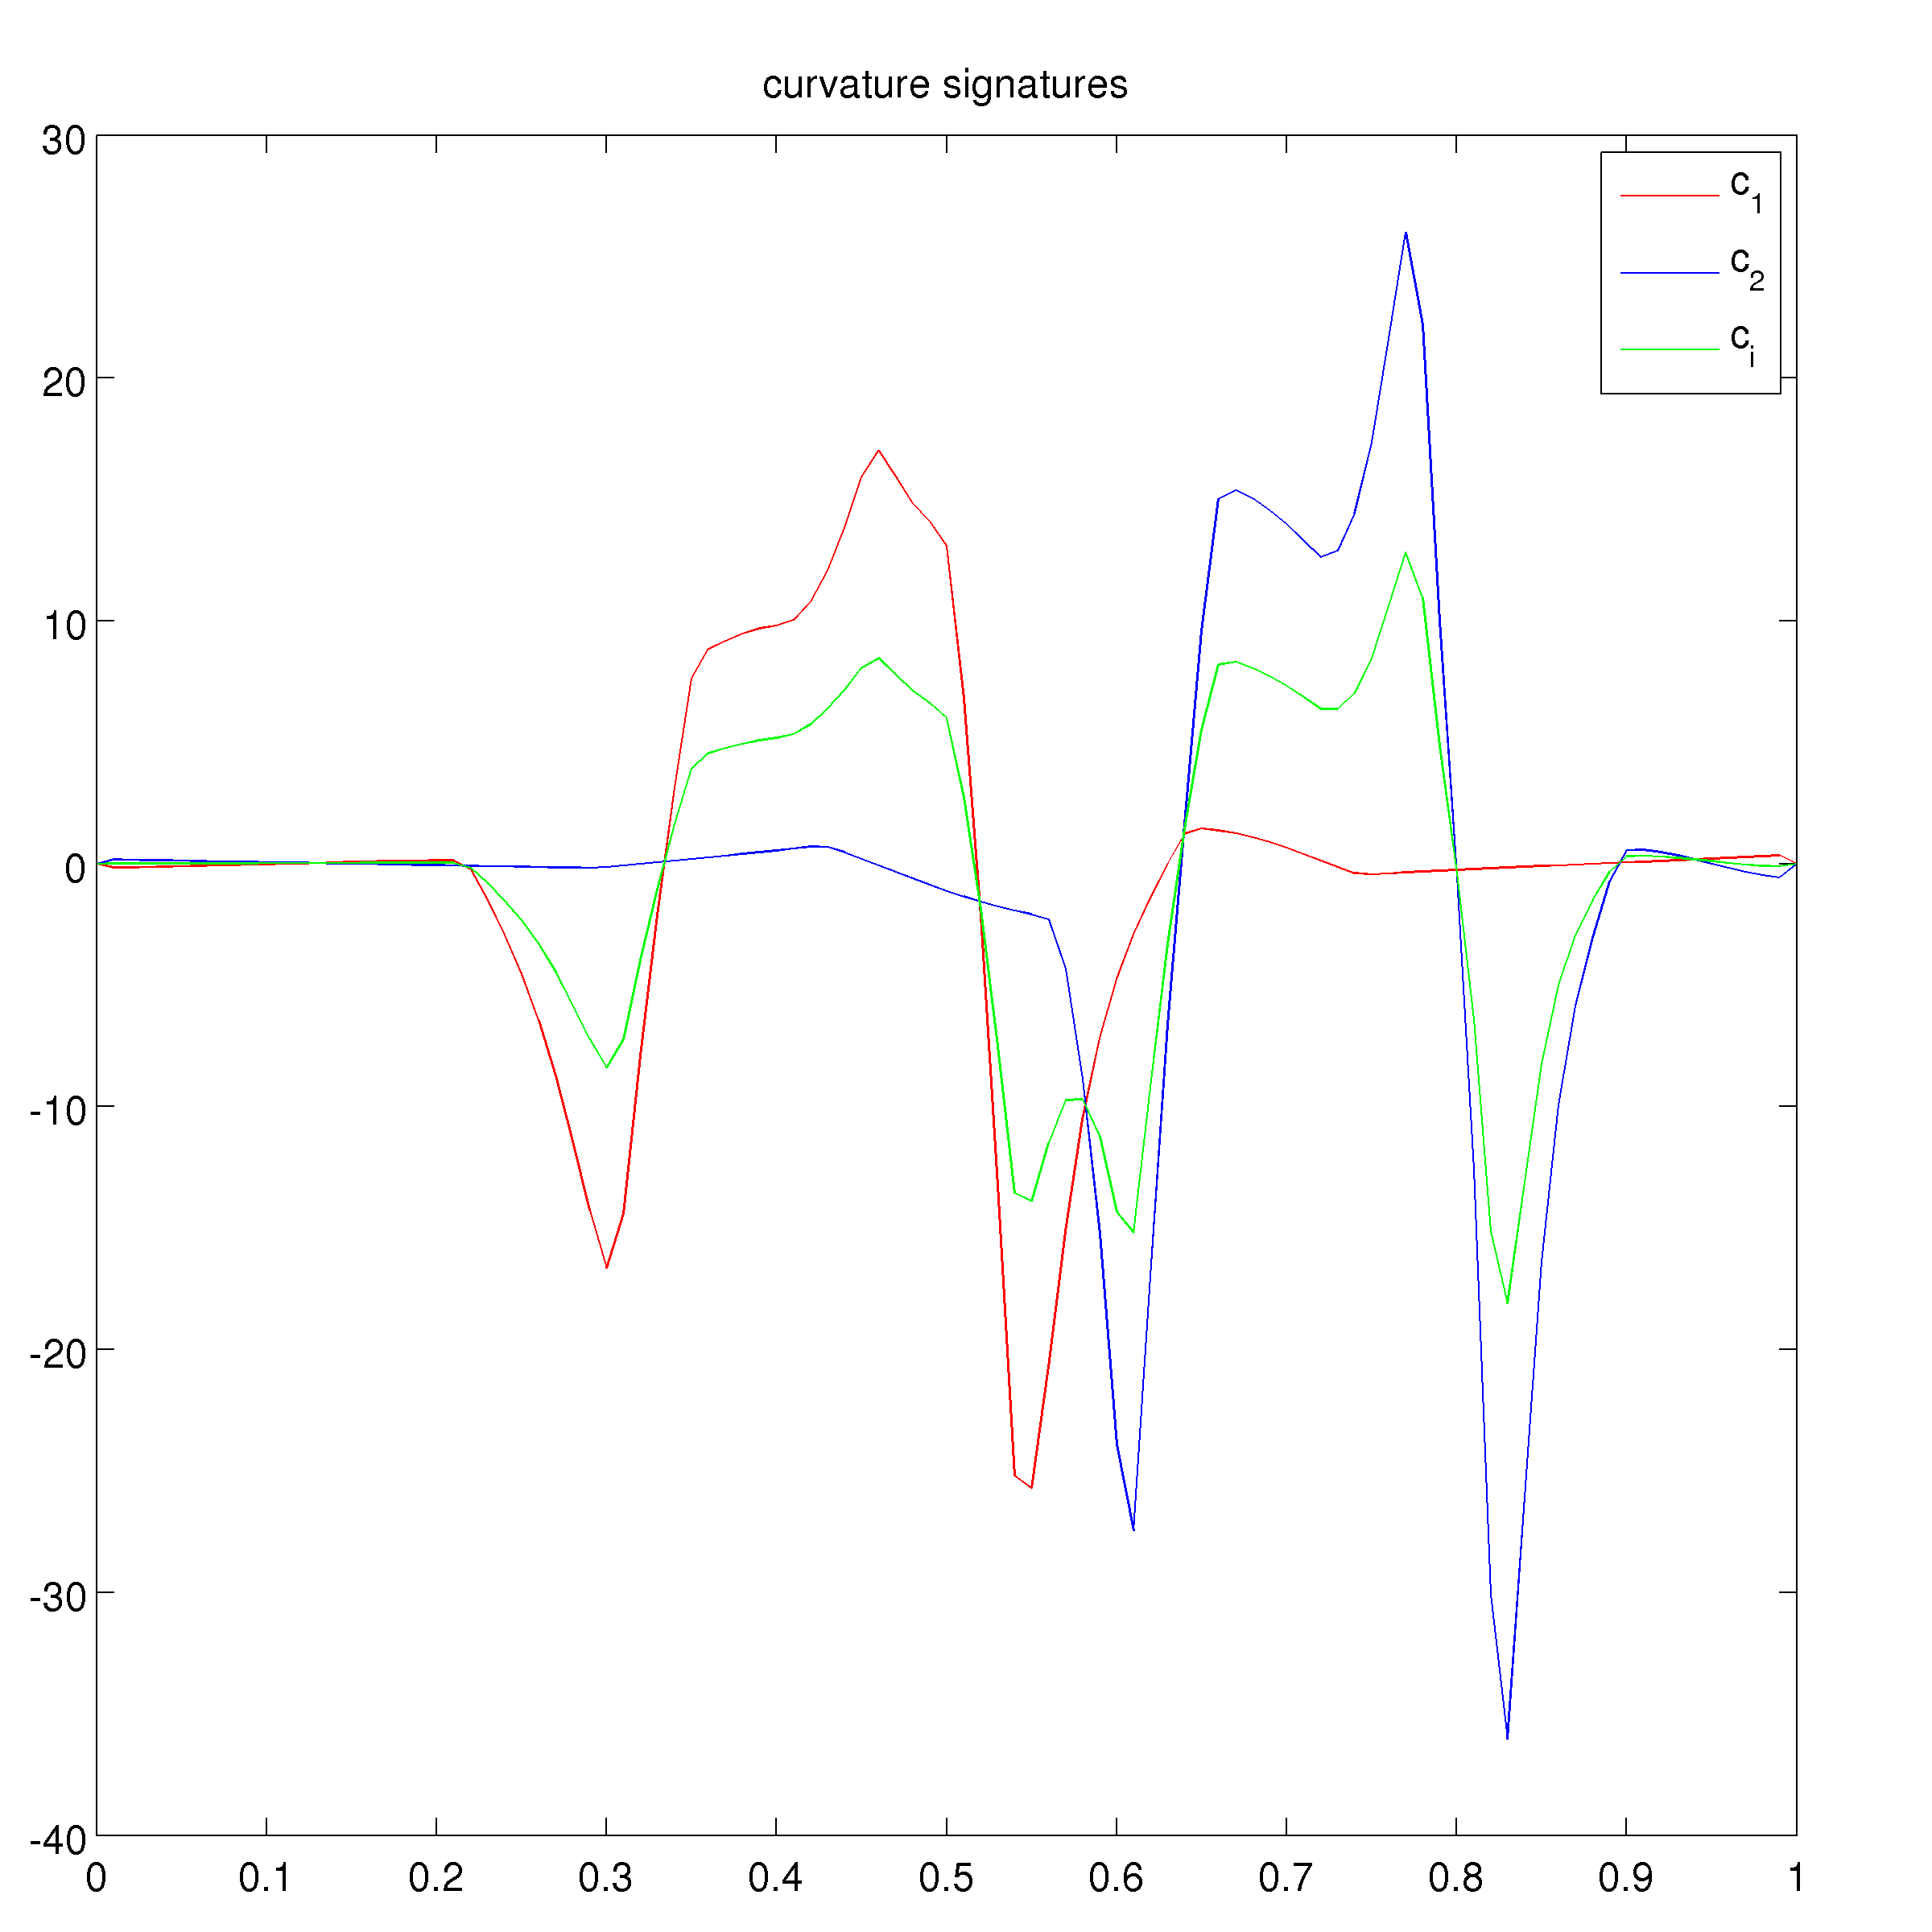
\includegraphics[width=\anchodos]{\chapFiveDir/results/curvature/example_02/curvature_signatures_interpolated.png}
		\label{fig:curve_interpolation:results:hat:interp:transform}
	}
		\subfloat[]{
		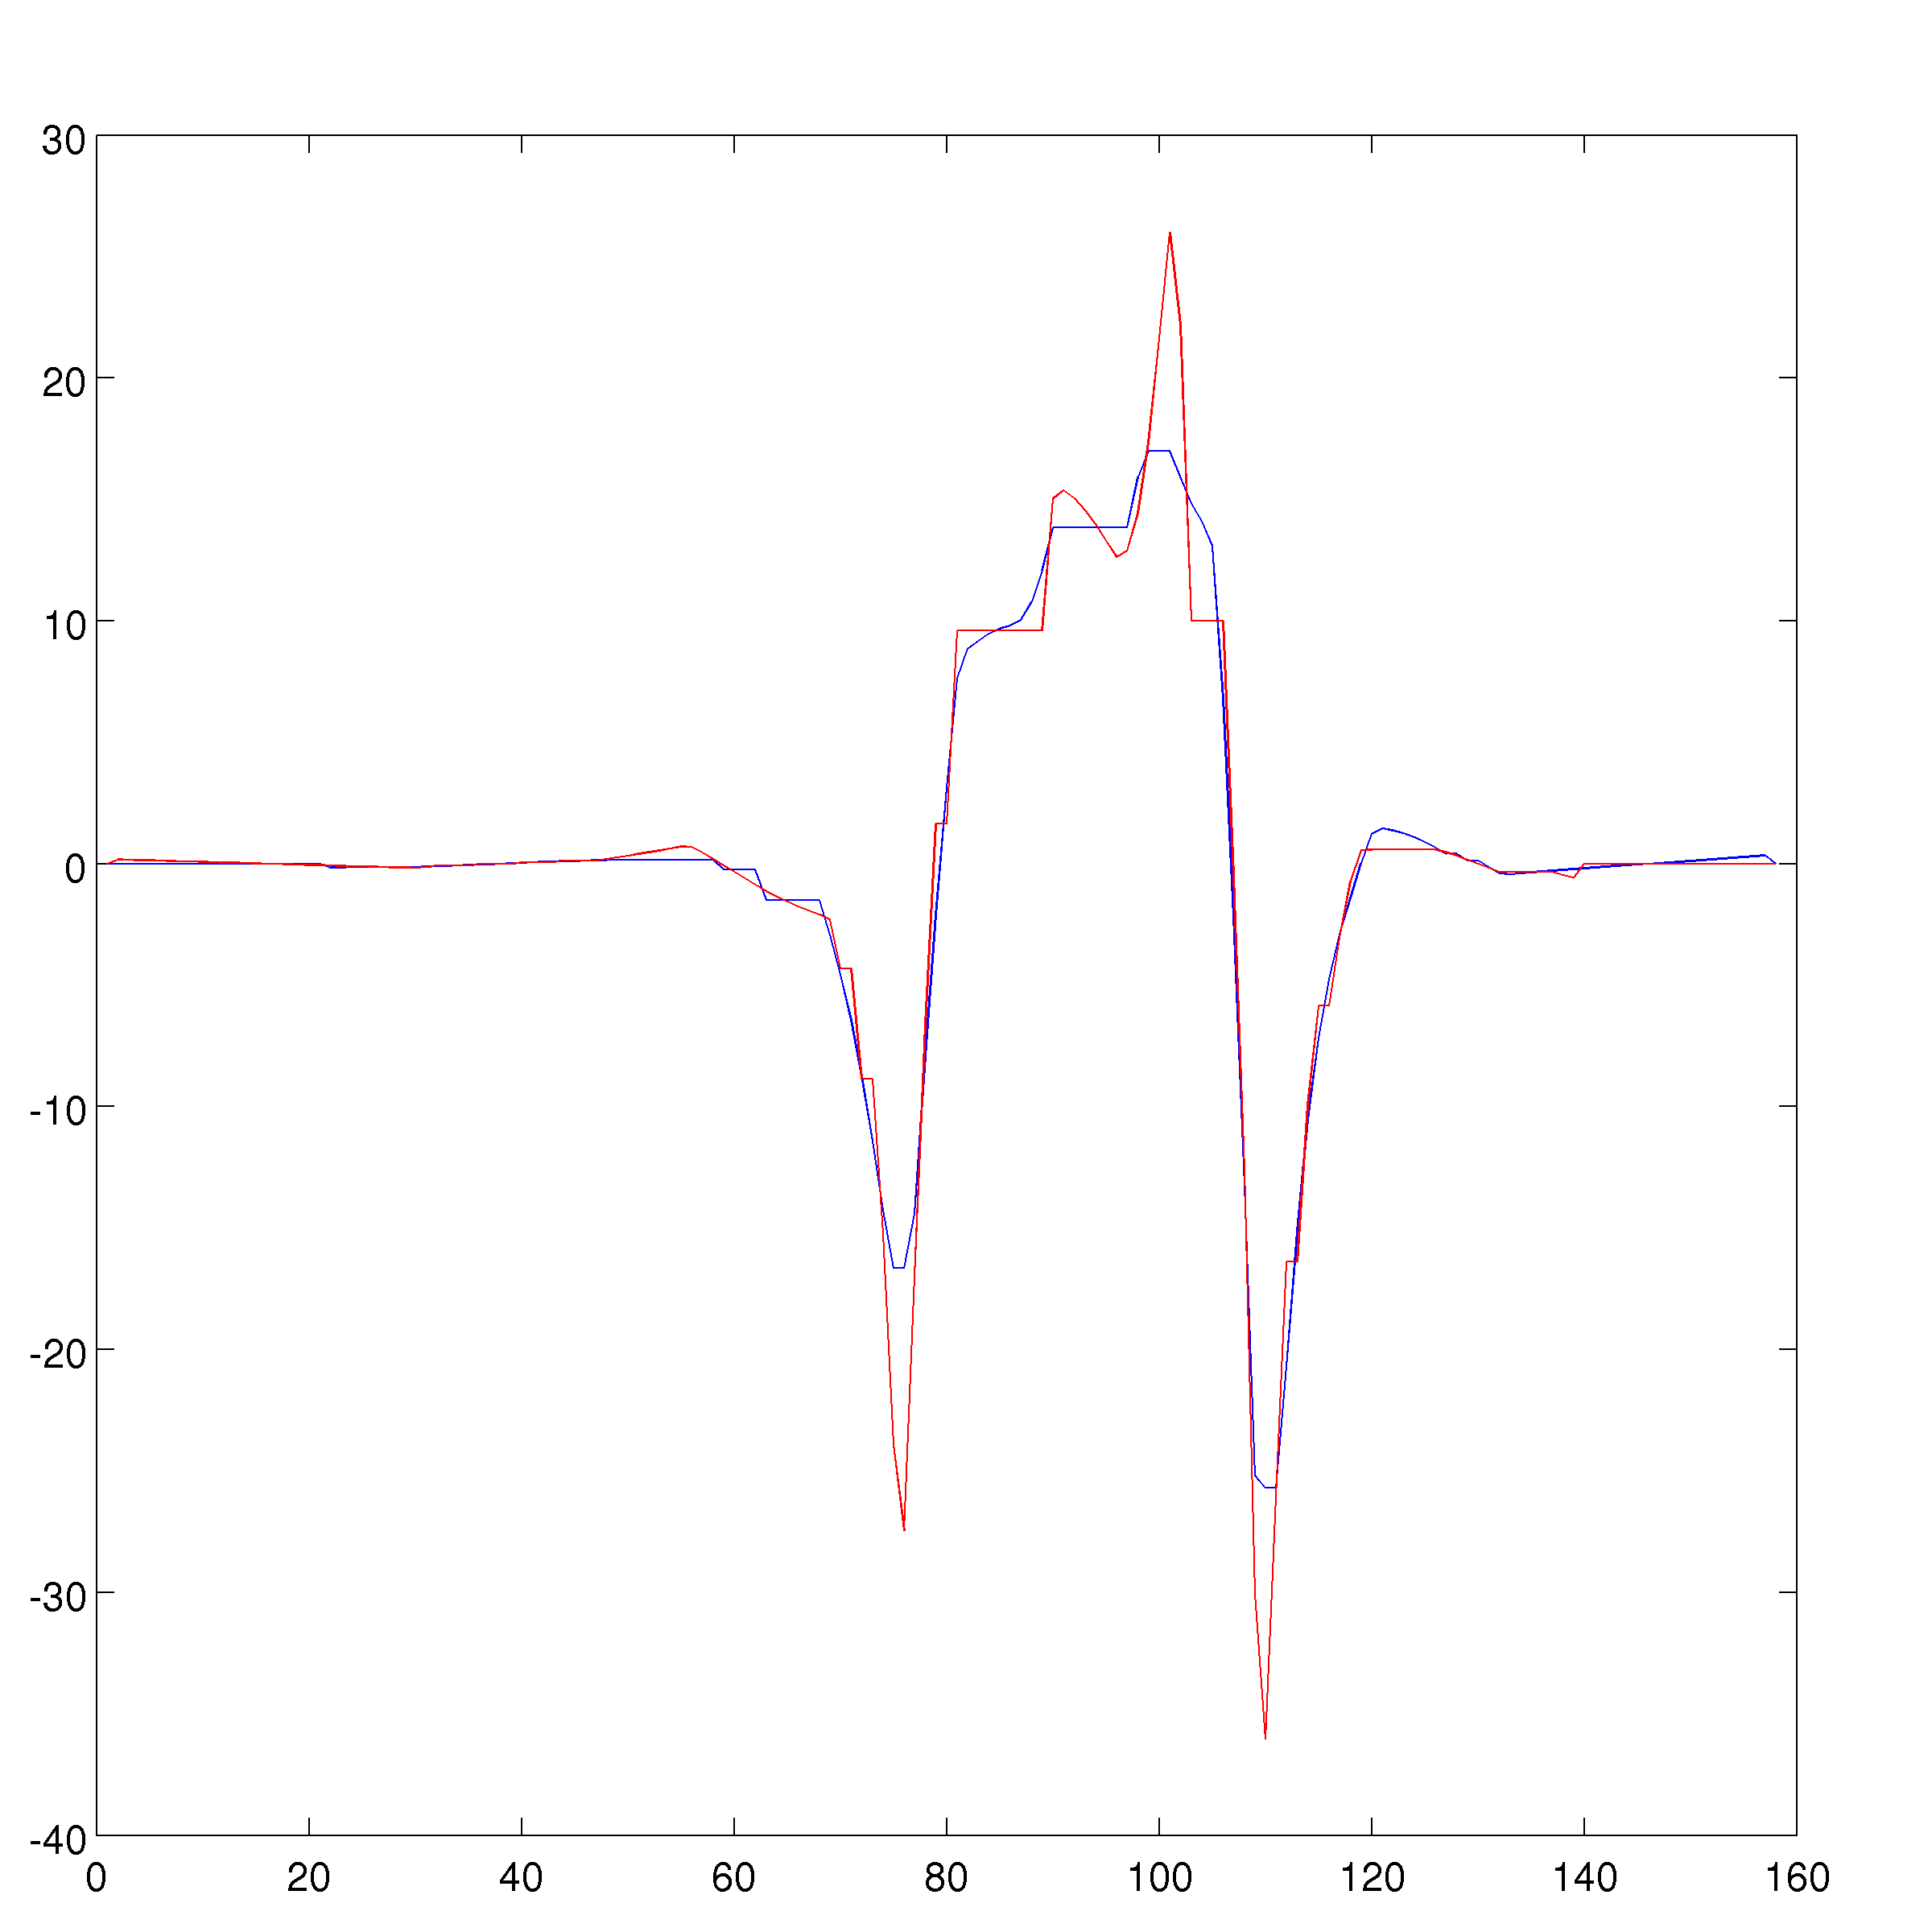
\includegraphics[width=\anchodos]{\chapFiveDir/results/curvature/example_02/dtw.png}
		\label{fig:curve_interpolation:results:hat:interp:basic:dtw}
	}
	\caption{Results of interpolating the curves of Figure \ref{fig:curve_interpolation:results:hat}. \protect\subref{fig:curve_interpolation:results:hat:interp:spatial} Original curves (red,blue) and interpolated curve (green) presenting two lobes. \protect\subref{fig:curve_interpolation:results:hat:interp:transform} Curvature signatures of the original curves (red,blue) and the interpolated one (green). \protect\subref{fig:curve_interpolation:results:hat:interp:basic:dtw} Dynamic Time Warping applied to curvature signature produces a very good matching between both.}
	\label{fig:curve_interpolation:results:hat:interp}
\end{figure}

\begin{figure}[h]
	\centering
	\subfloat[]{
		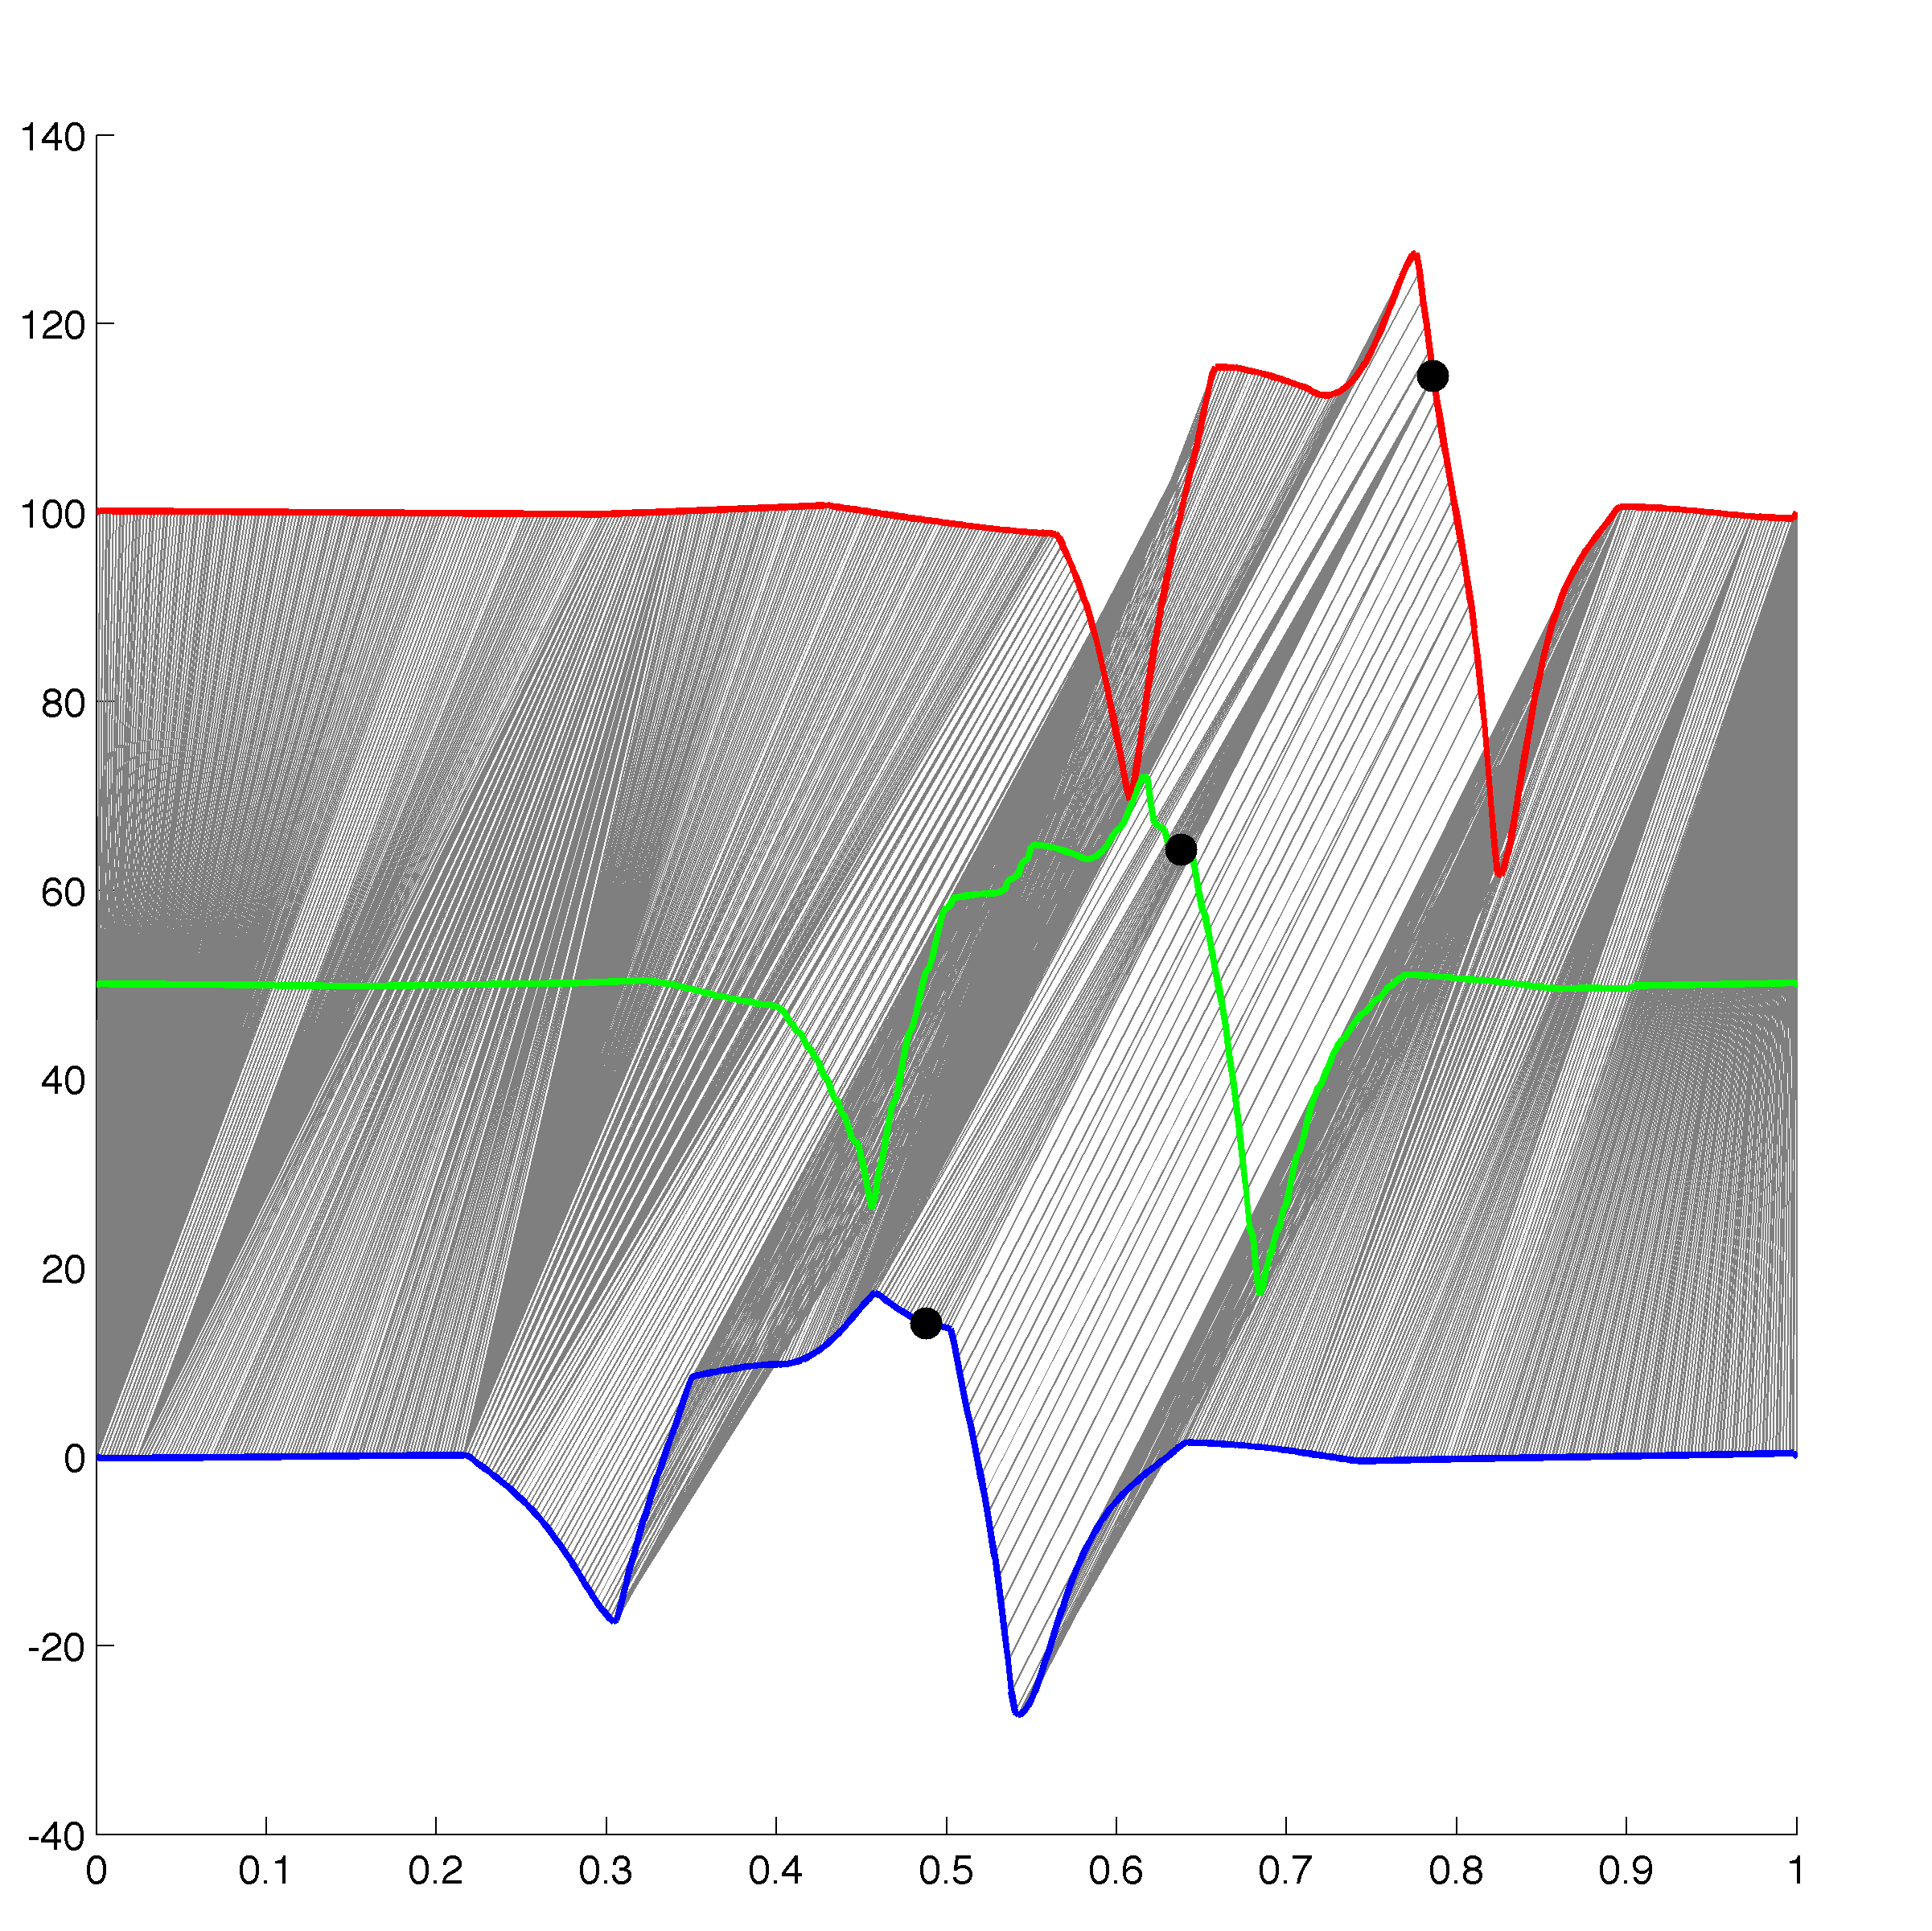
\includegraphics[width=\anchodos]{\chapFiveDir/results/curvature/example_02/curvature_interpolated_dtw_transform}
		\label{fig:curve_interpolation:results:hat:interp:dtw:transform}
	}
	\subfloat[]{
		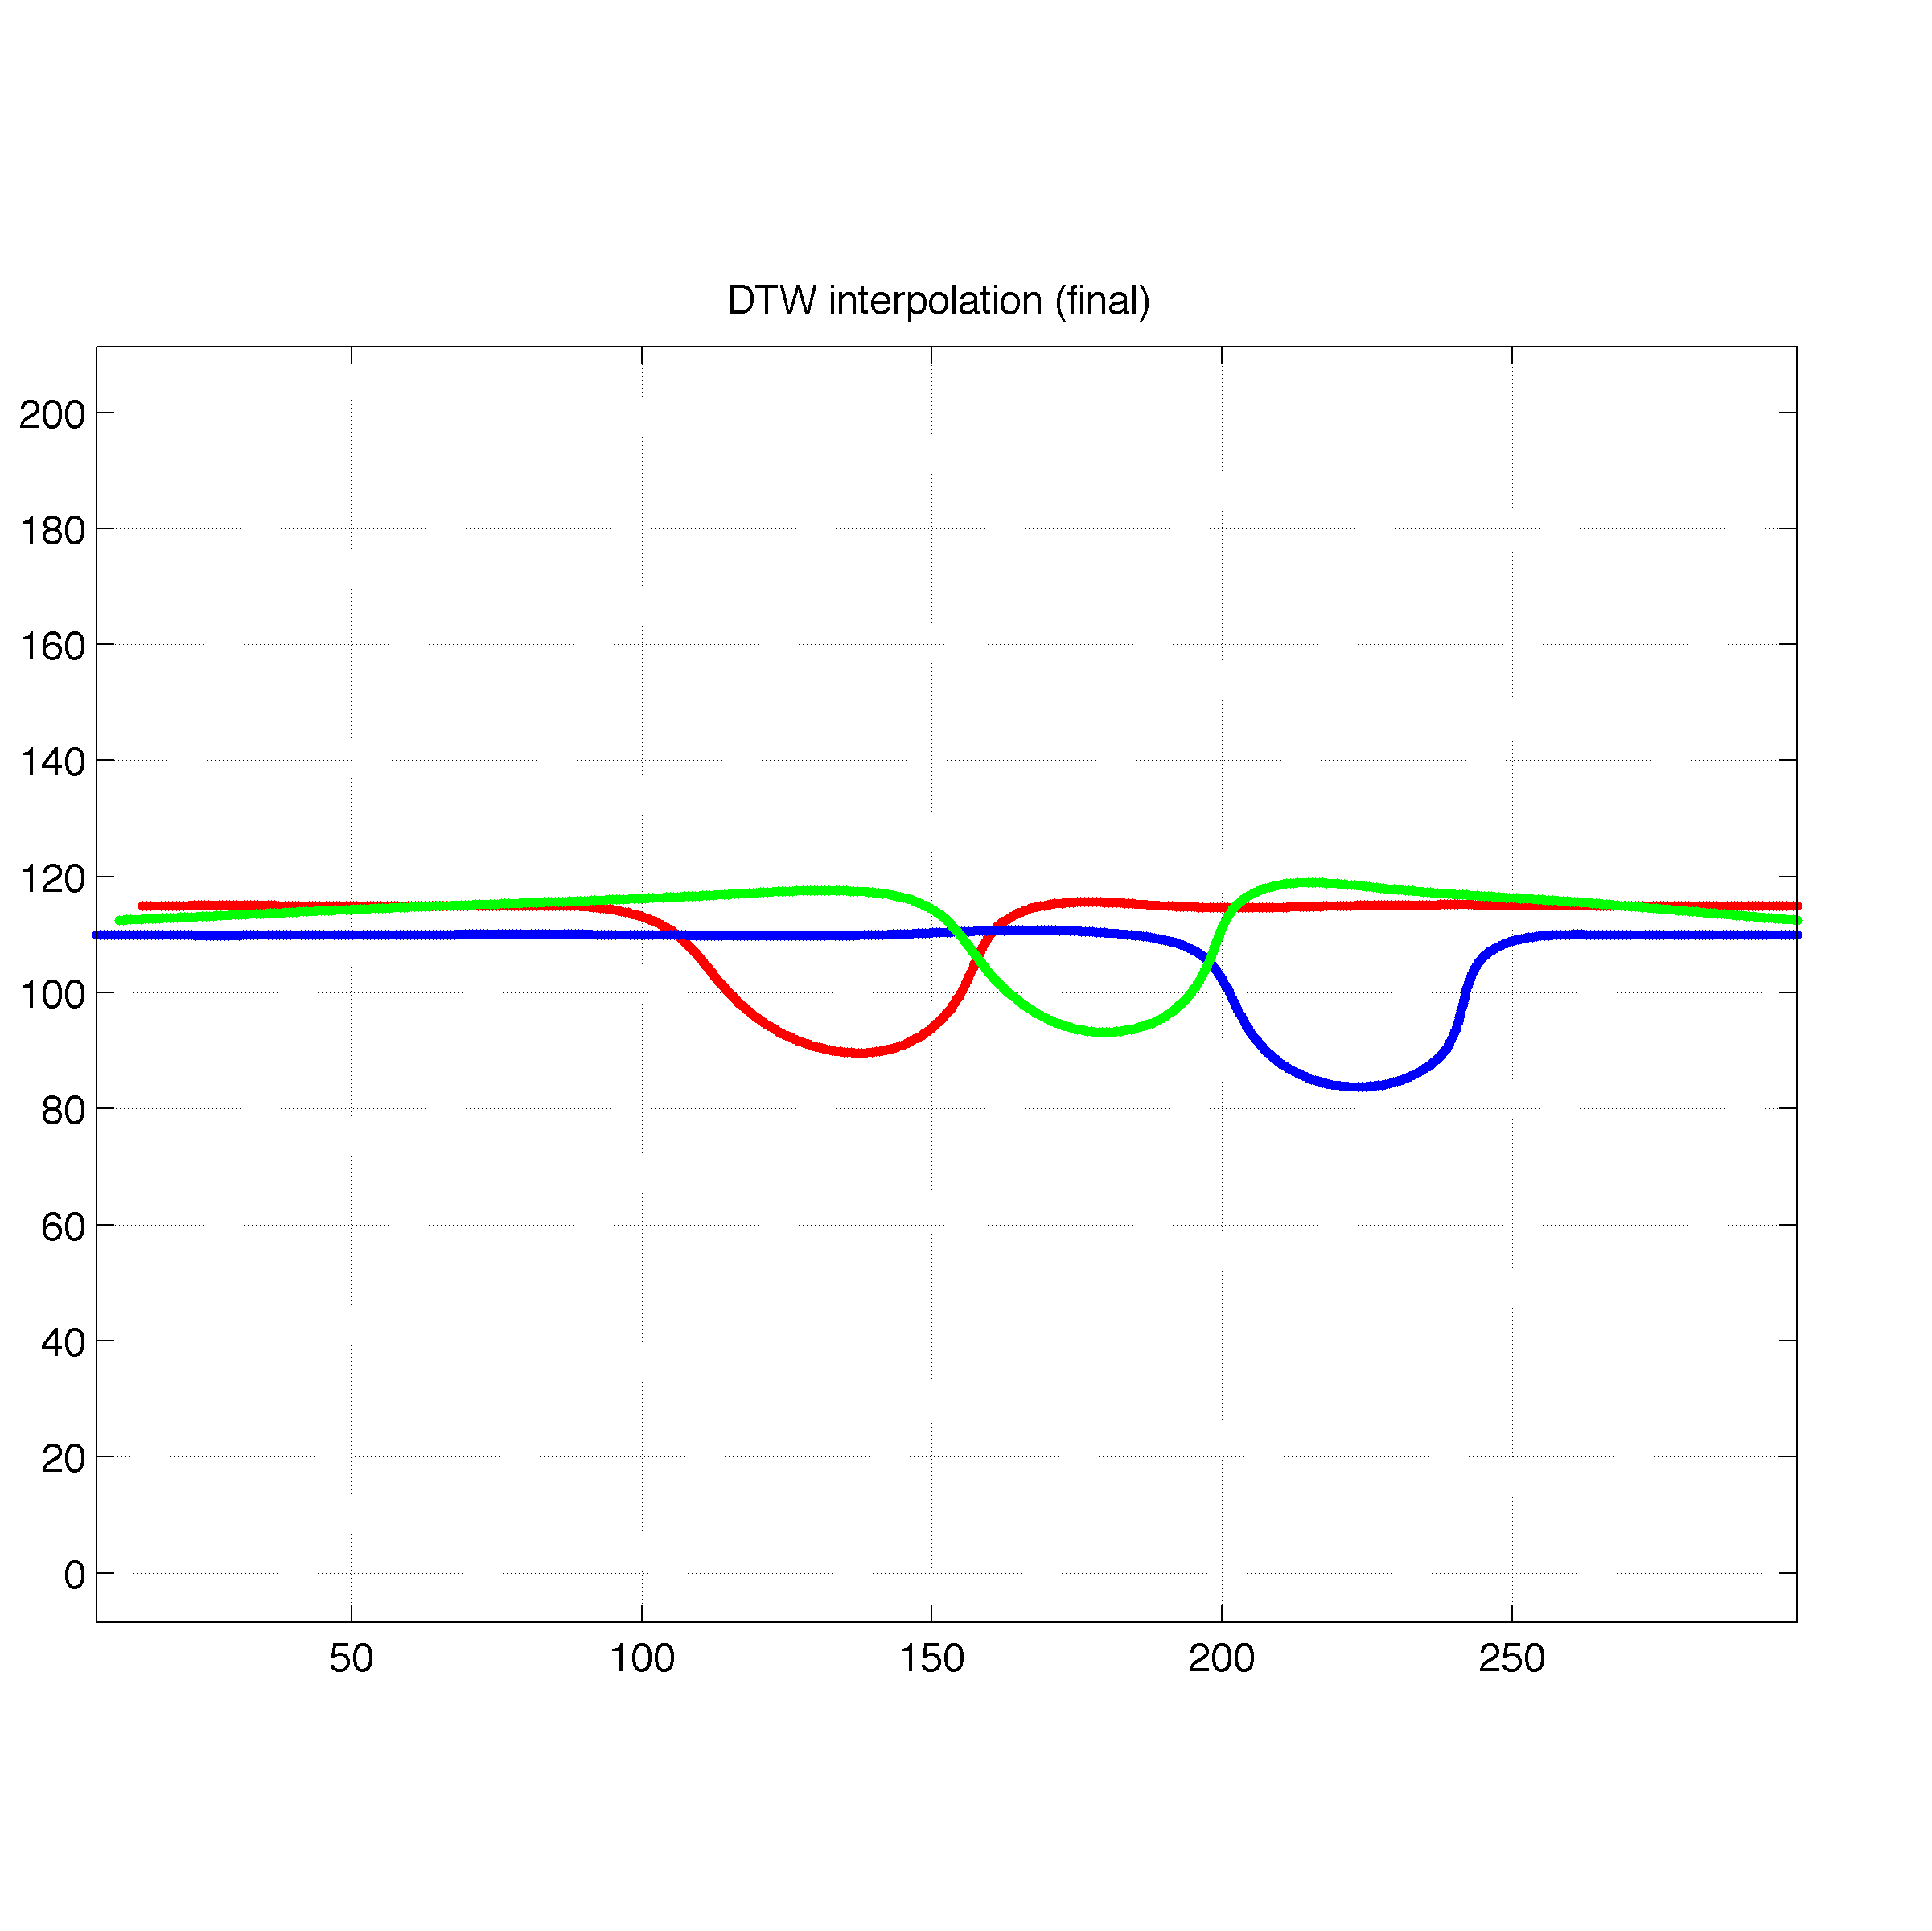
\includegraphics[width=\anchodos]{\chapFiveDir/results/curvature/example_02/curvature_interpolated_dtw_spatial}
		\label{fig:curve_interpolation:results:hat:interp:dtw:spatial}
	}
	\caption{Results of interpolating the curves of Figure \ref{fig:curve_interpolation:results:hat} using the curvature transform and Dynamic Time Warping (DTW).
		\protect\subref{fig:curve_interpolation:results:hat:interp:dtw:transform} Dynamic Time Warping applied to curvature signature produces a very good matching between both curvature signatures. The original curve signatures are shown in red and blue and the interpolated one is shown in green. The dark dot represent one corresponding point in each curve. \protect\subref{fig:curve_interpolation:results:hat:interp:spatial} Original curves (red,blue) and interpolated curve (green) presenting only one lobe at an intermediate point between the original ones. \label{fig:curve_interpolation:results:hat:interp:dtw}
	}
\end{figure}

\subsection{Implementation}

The algorithm presented in previous section was developed completely in Matlab, using only basic builtin functions. For the high-order numerical schemes we used Matlab's implementation of a Runge-Kutta (4,5) scheme available in the ode45 function. Our code is freely available to download \footnote{Download Matlab code from \url{https://gitlab.com/ingenieriabiologica/phd/curves}.} in order to ease the reproducibility of the presented results.
In addition, we provide an online demo \footnote{Available at the IPOL Journal \url{http://ipolcore.ipol.im/demo/clientApp/demo.html?id=77777000028}} were the algorithm can be tested with the provided data or by uploading your own experiments, without having to install or code anything.
The implemented algorithm runs in 0.09s for a pair of 100 point curves on a standard \verb+Intel(R) Core(TM) i7-3770 CPU @ 3.40GHz+ PC with 16GiB RAM, using Matlab R2014a.

\clearpage
\section{Results}

In previous sections we have shown basic results of the curvature transform in the case of parametric curves, where we computed the curvature signature from the spatial representation of the curve and the shown inverse process of reconstructing the curve from the signature.

We extend those results by interpolating two smooth parametric curves: a Cornu Spiral defined as the curve such that $\kappa(s)=s$ and a quarter circle with $\kappa(s)=1$, as shown in Figures \ref{fig:curve_interpolation:results:cornu_spiral} and \ref{fig:curve_interpolation:results:quarter} respectively.

The results of the interpolation are shown in Figure \ref{fig:curve_interpolation:results:parametric:animation} were we show the interpolation results at various intermediate steps and we compare the curvature interpolation with the direct interpolation of the spatial points. In the first case, interpolation works as expected, unfolding the spiral and maintaining the smoothness of the intermediate curve at every step. 
In the second case, direct interpolation on the spatial domain produces non smooth curves that develop self-intersections.

\begin{figure}[h]
	\centering
		\subfloat[]{
		\includegraphics[width=\anchodos]{\chapFiveDir/results/c1.png}
		\label{fig:curve_interpolation:results:cornu_spiral}
	}
	\subfloat[]{
		\includegraphics[width=\anchodos]{\chapFiveDir/results/c2.png}
		\label{fig:curve_interpolation:results:quarter}
	}
	\caption{Example 1: Input curves. \protect\subref{fig:curve_interpolation:results:cornu_spiral} Cornu Spiral \protect\subref{fig:curve_interpolation:results:quarter} Quarter circle.}
	\label{fig:curve_interpolation:results:parametric}
\end{figure}	

\begin{figure}[h]
	\centering
	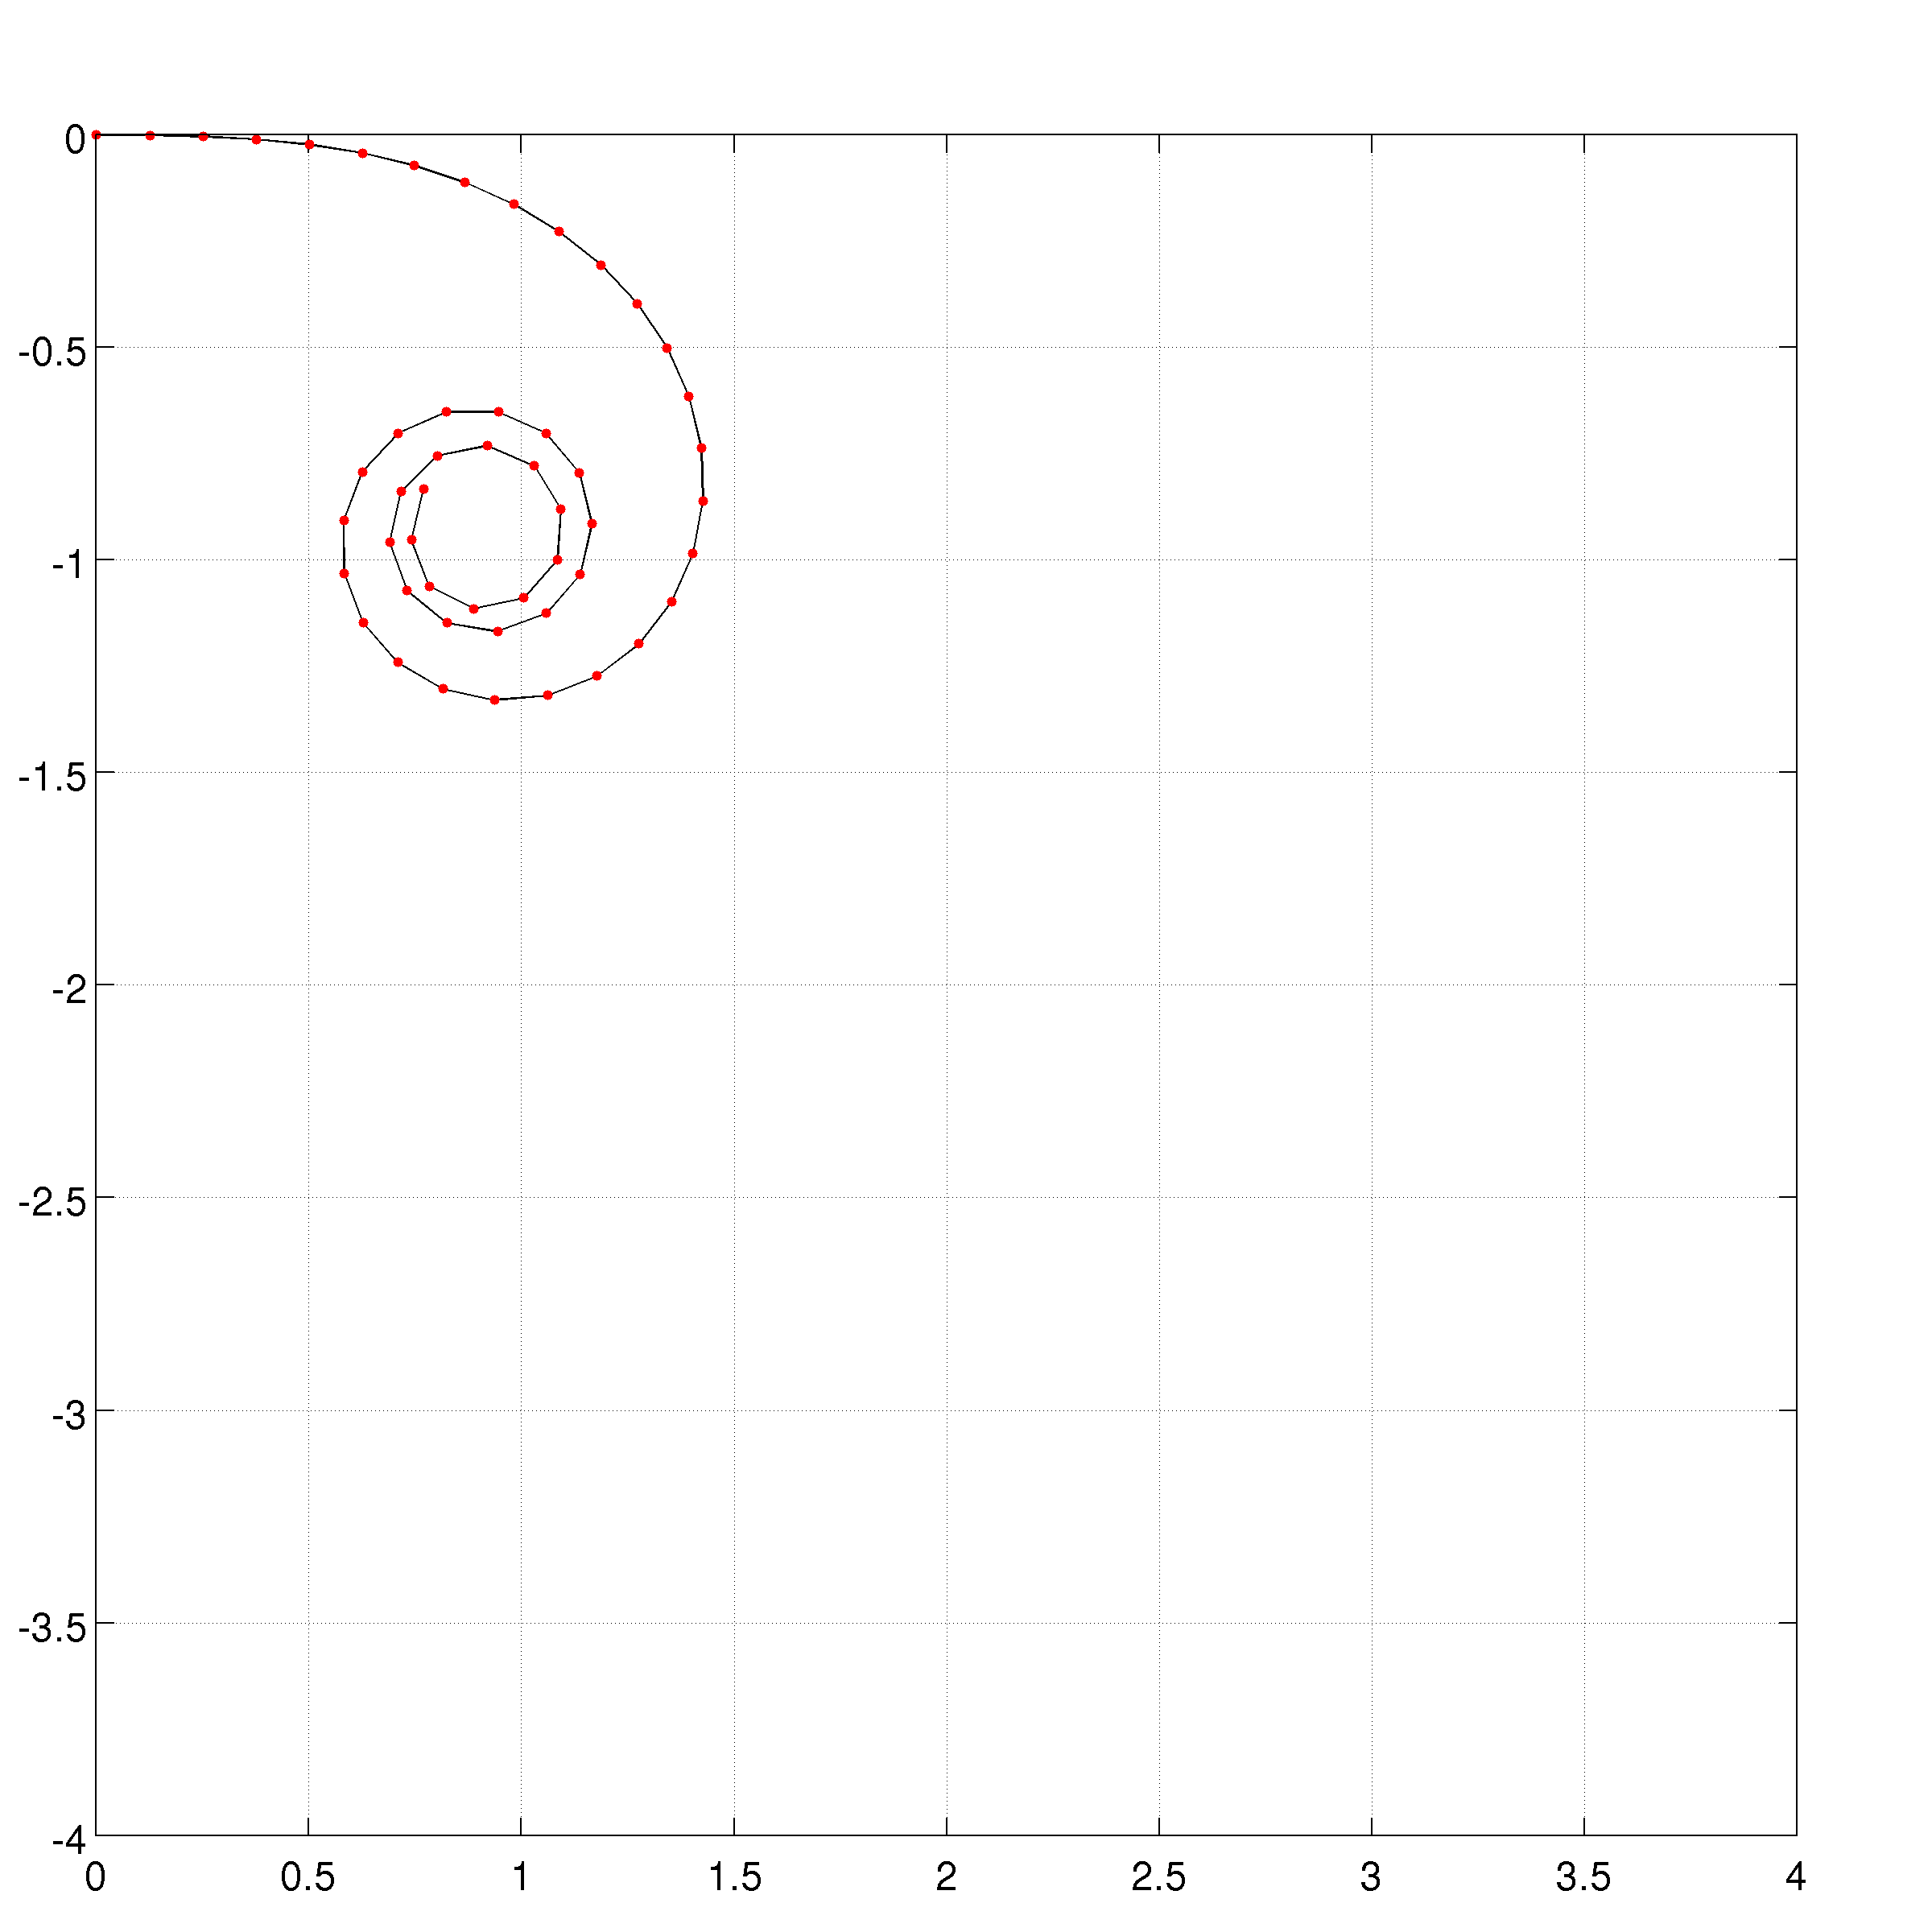
\includegraphics[width=\anchoseis]{\chapFiveDir/results/curvature/example_01/ani_curve_0.10.png}
	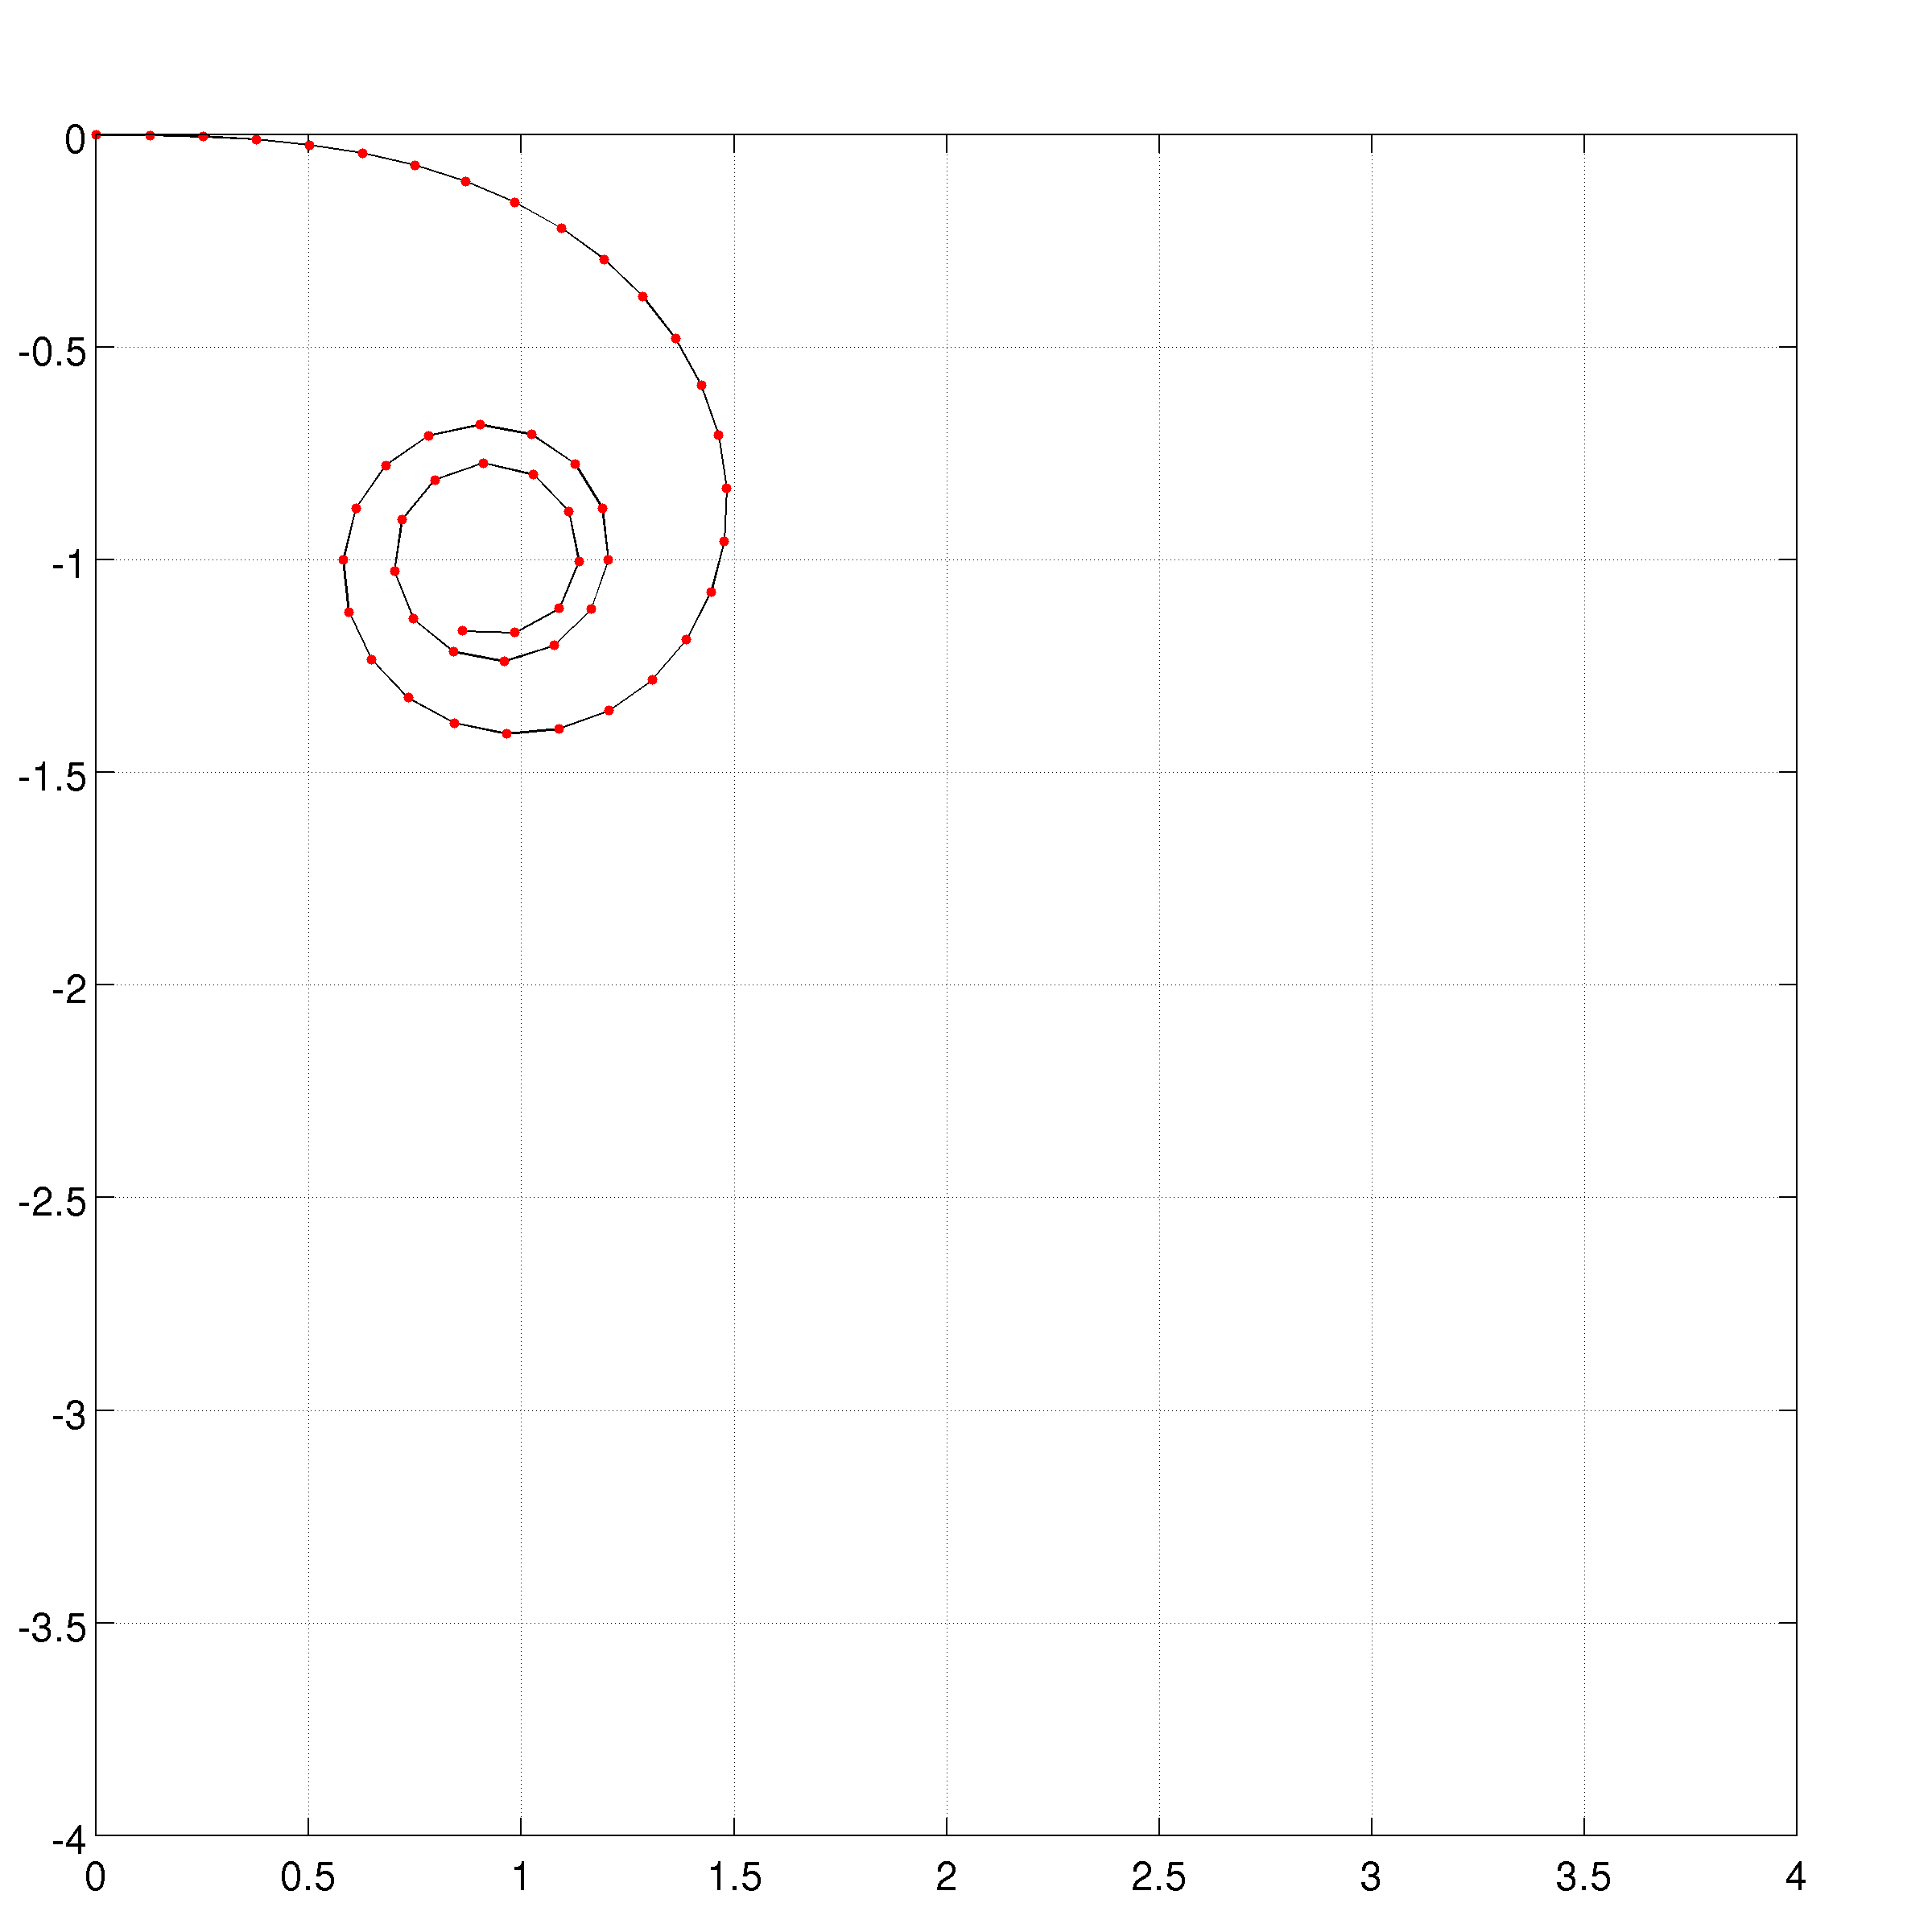
\includegraphics[width=\anchoseis]{\chapFiveDir/results/curvature/example_01/ani_curve_0.20.png}
	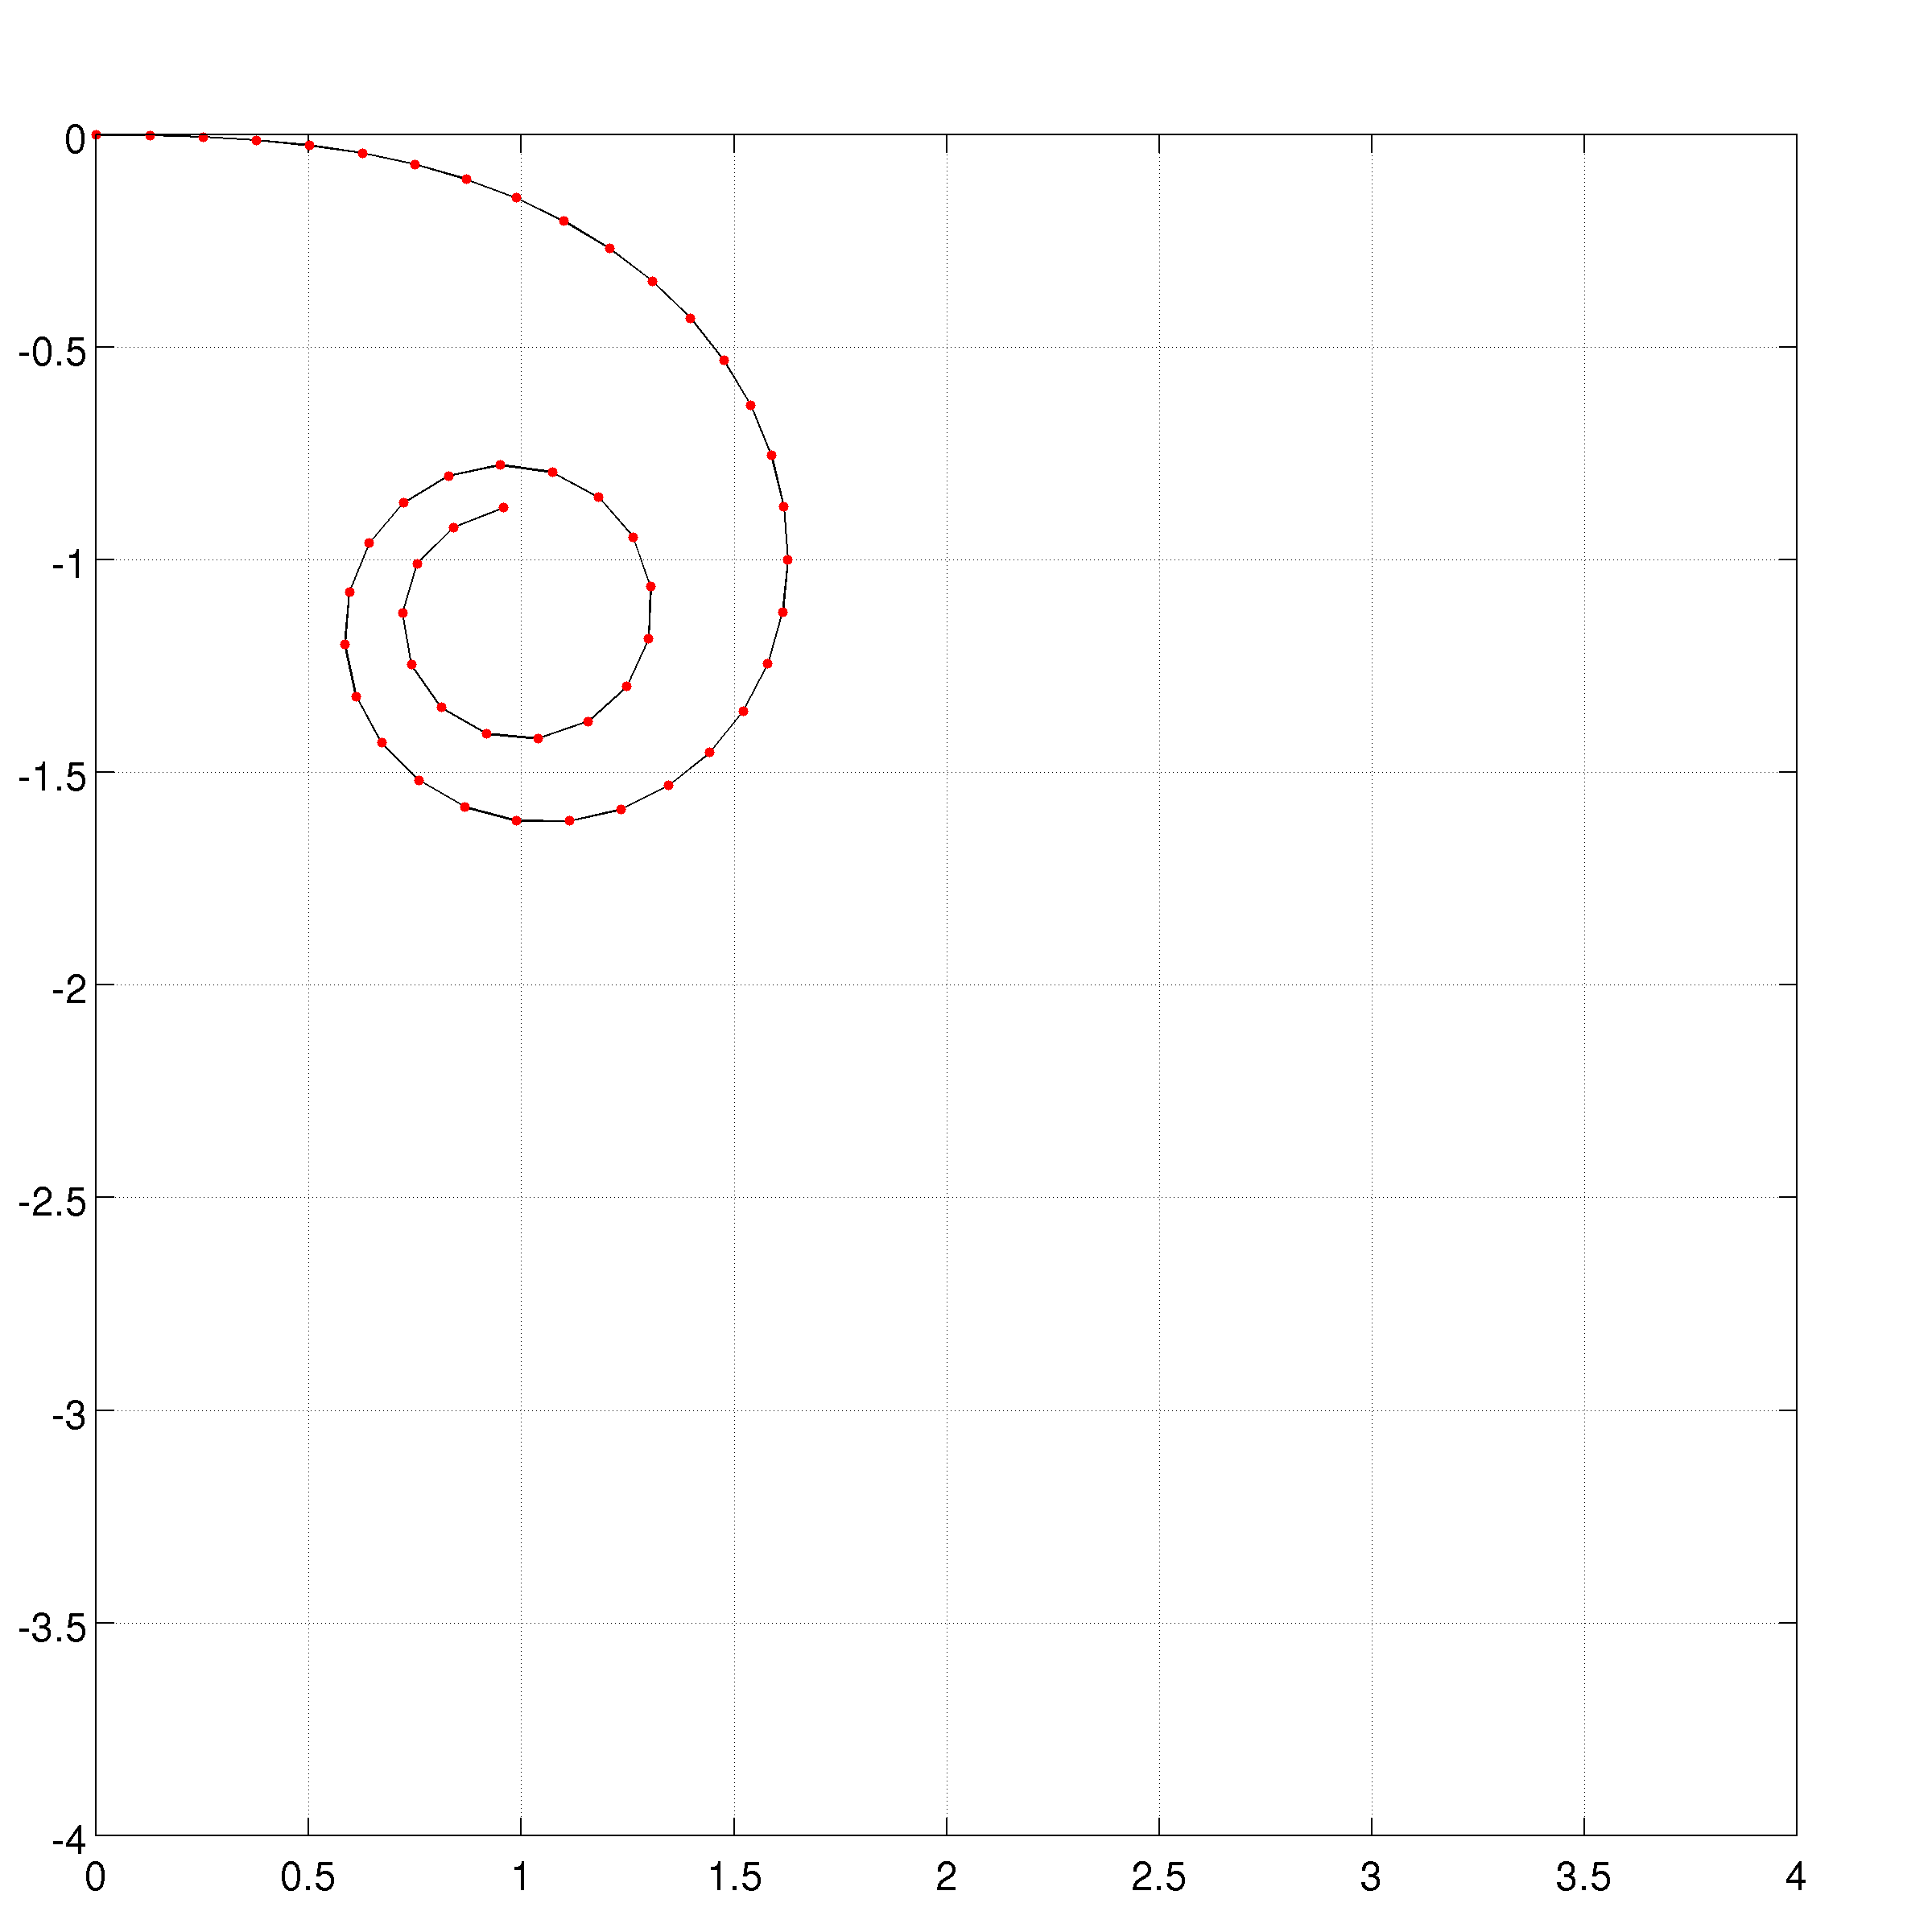
\includegraphics[width=\anchoseis]{\chapFiveDir/results/curvature/example_01/ani_curve_0.40.png}
	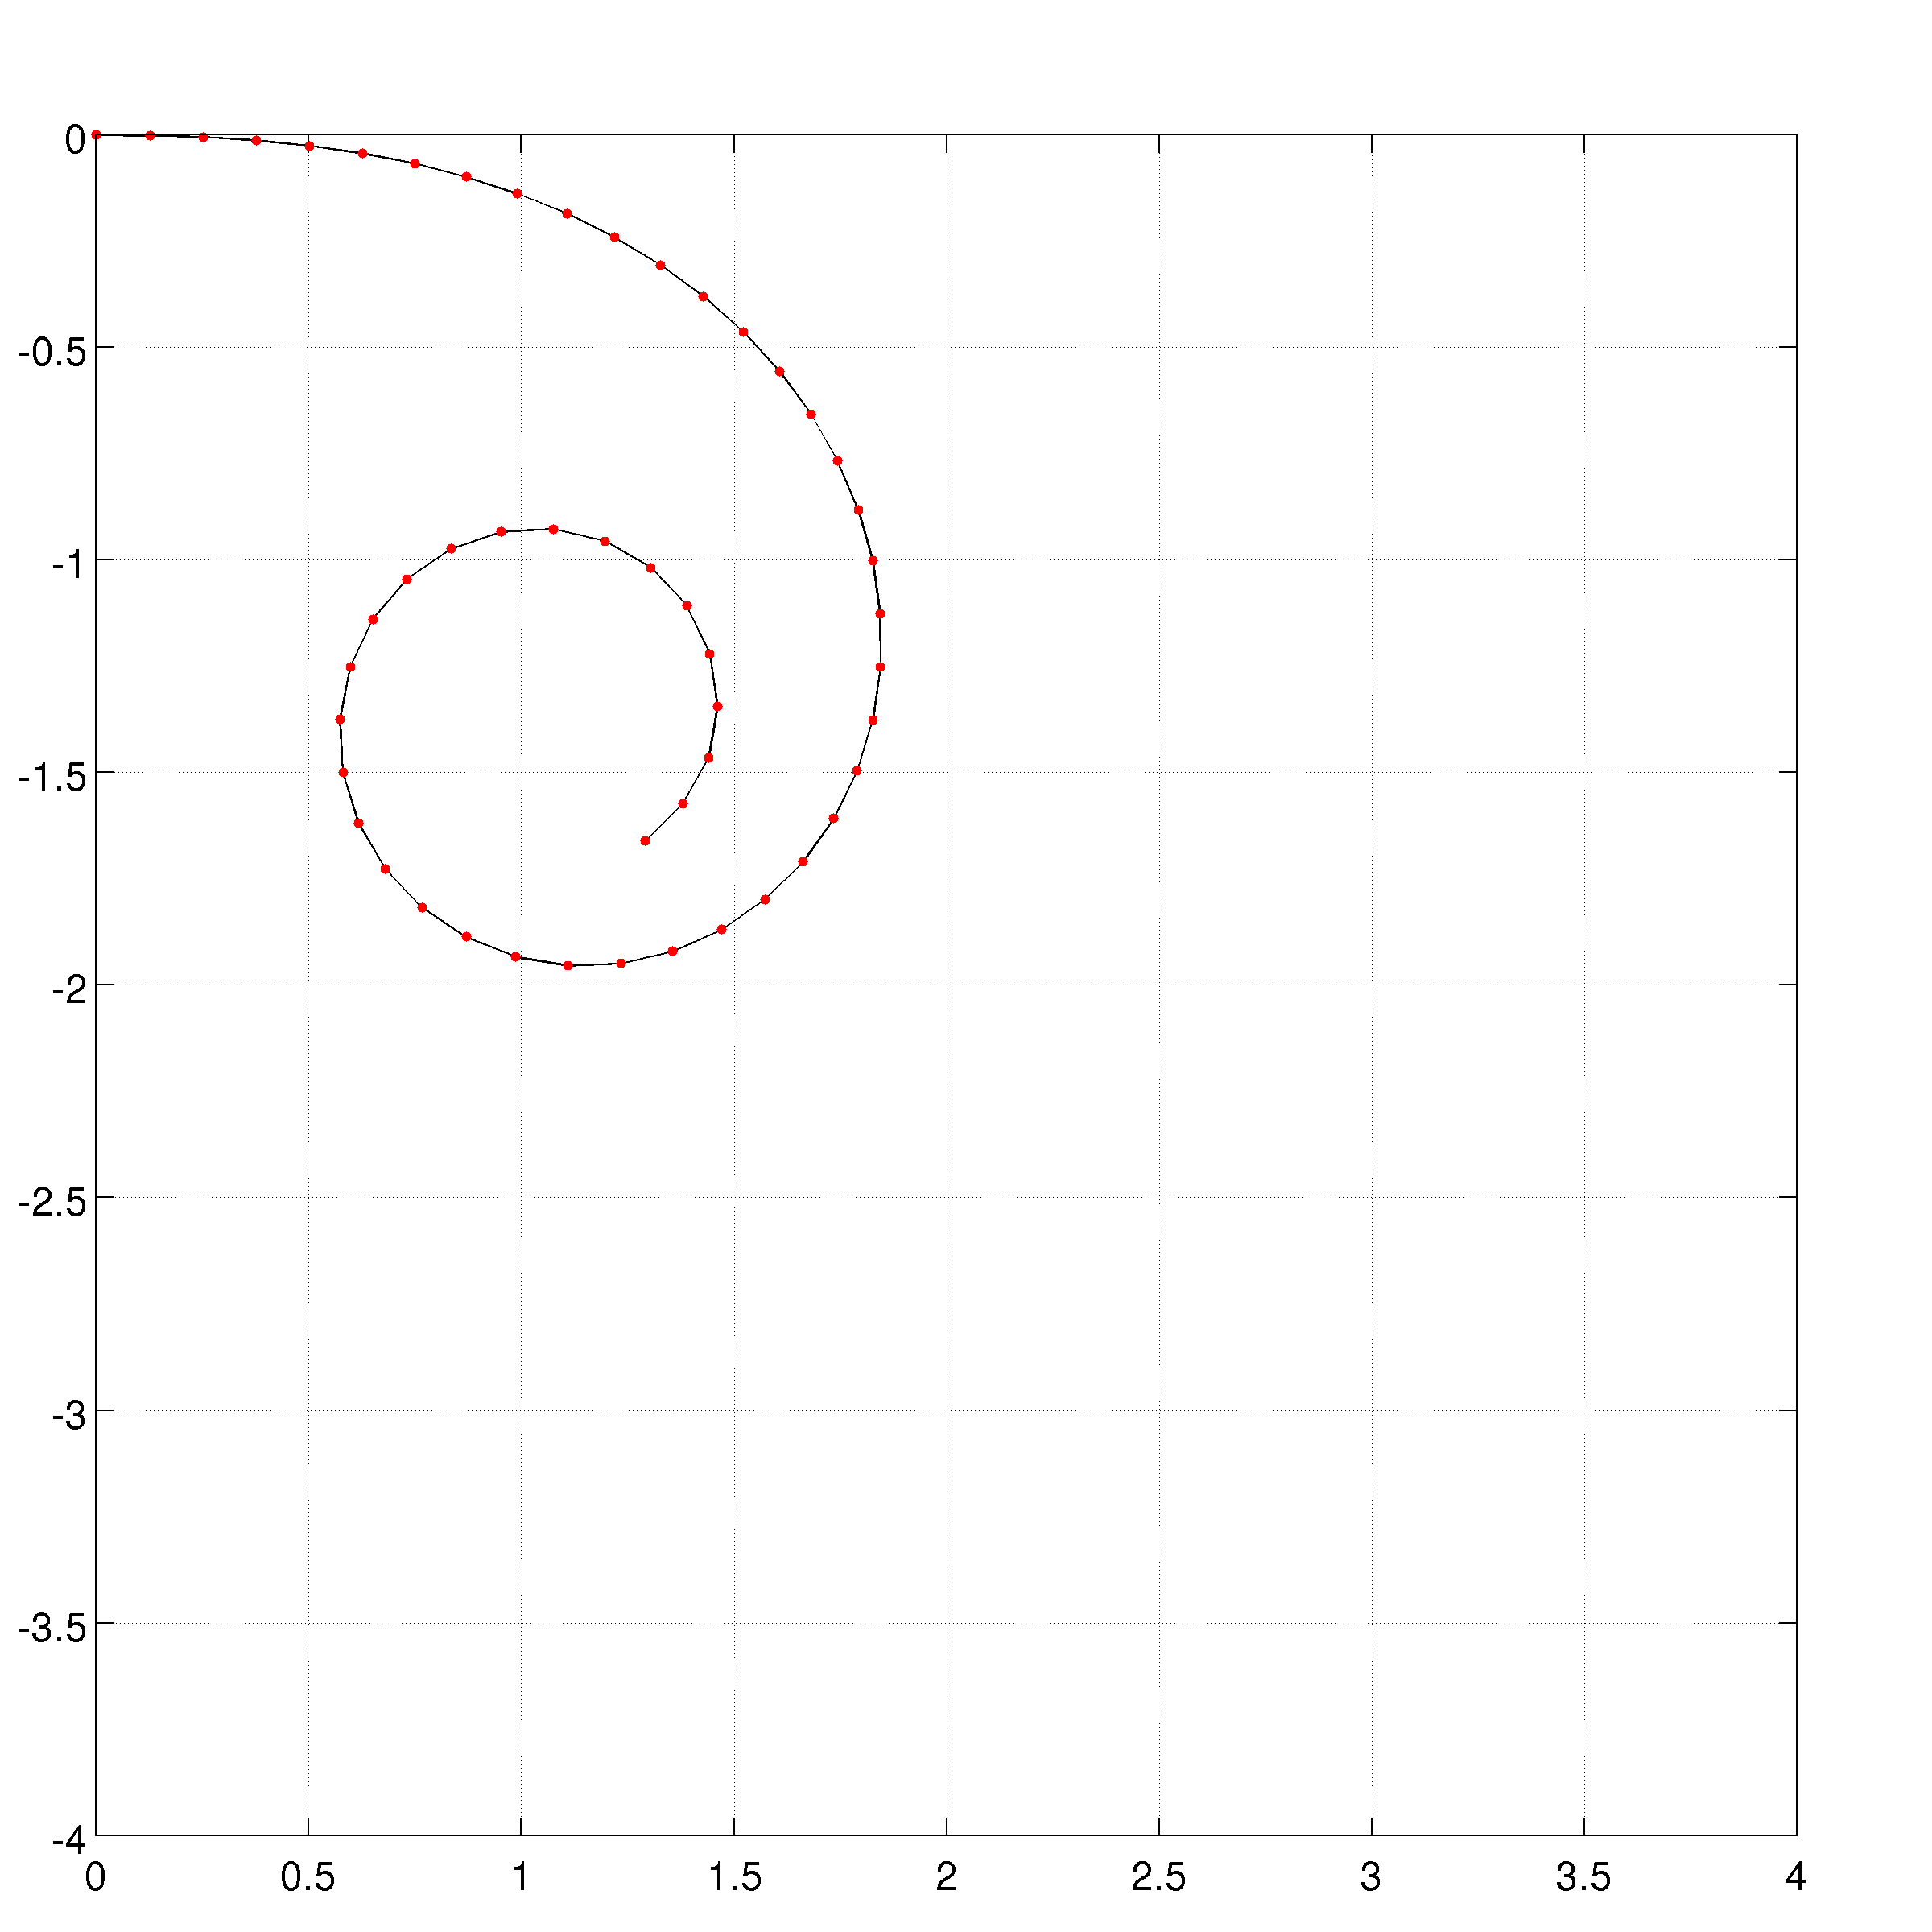
\includegraphics[width=\anchoseis]{\chapFiveDir/results/curvature/example_01/ani_curve_0.60.png}
	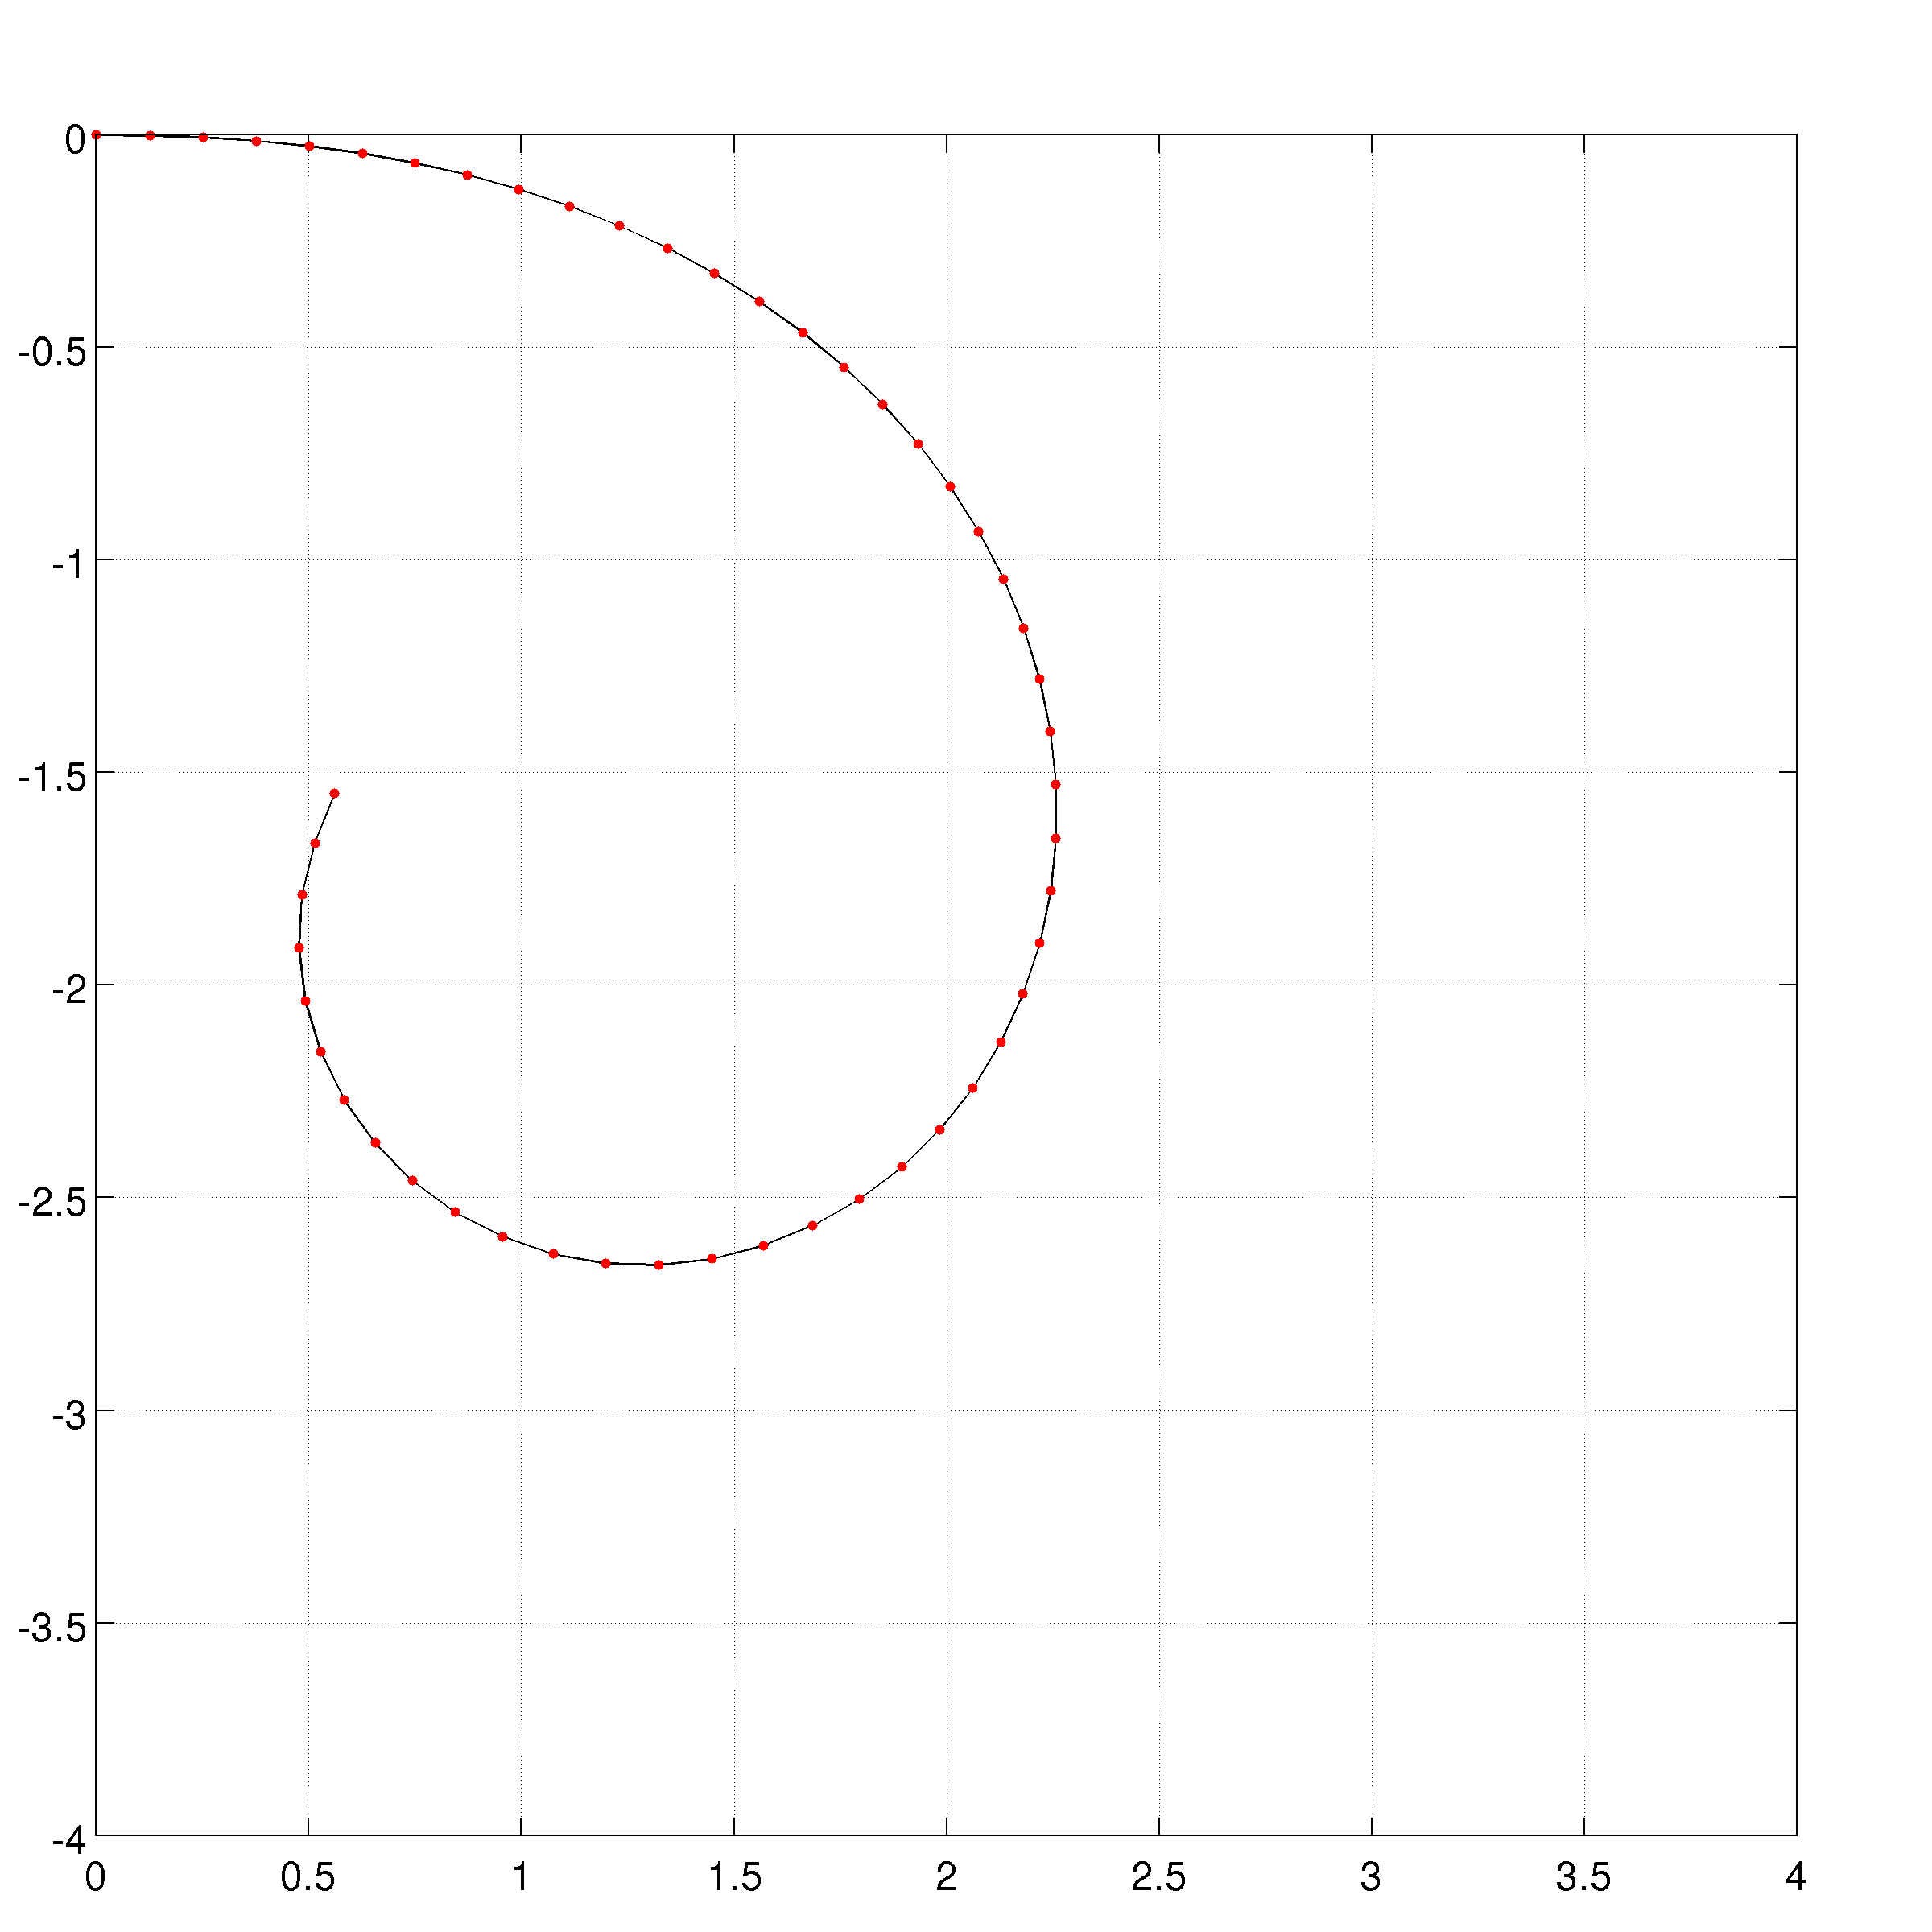
\includegraphics[width=\anchoseis]{\chapFiveDir/results/curvature/example_01/ani_curve_0.80.png}
	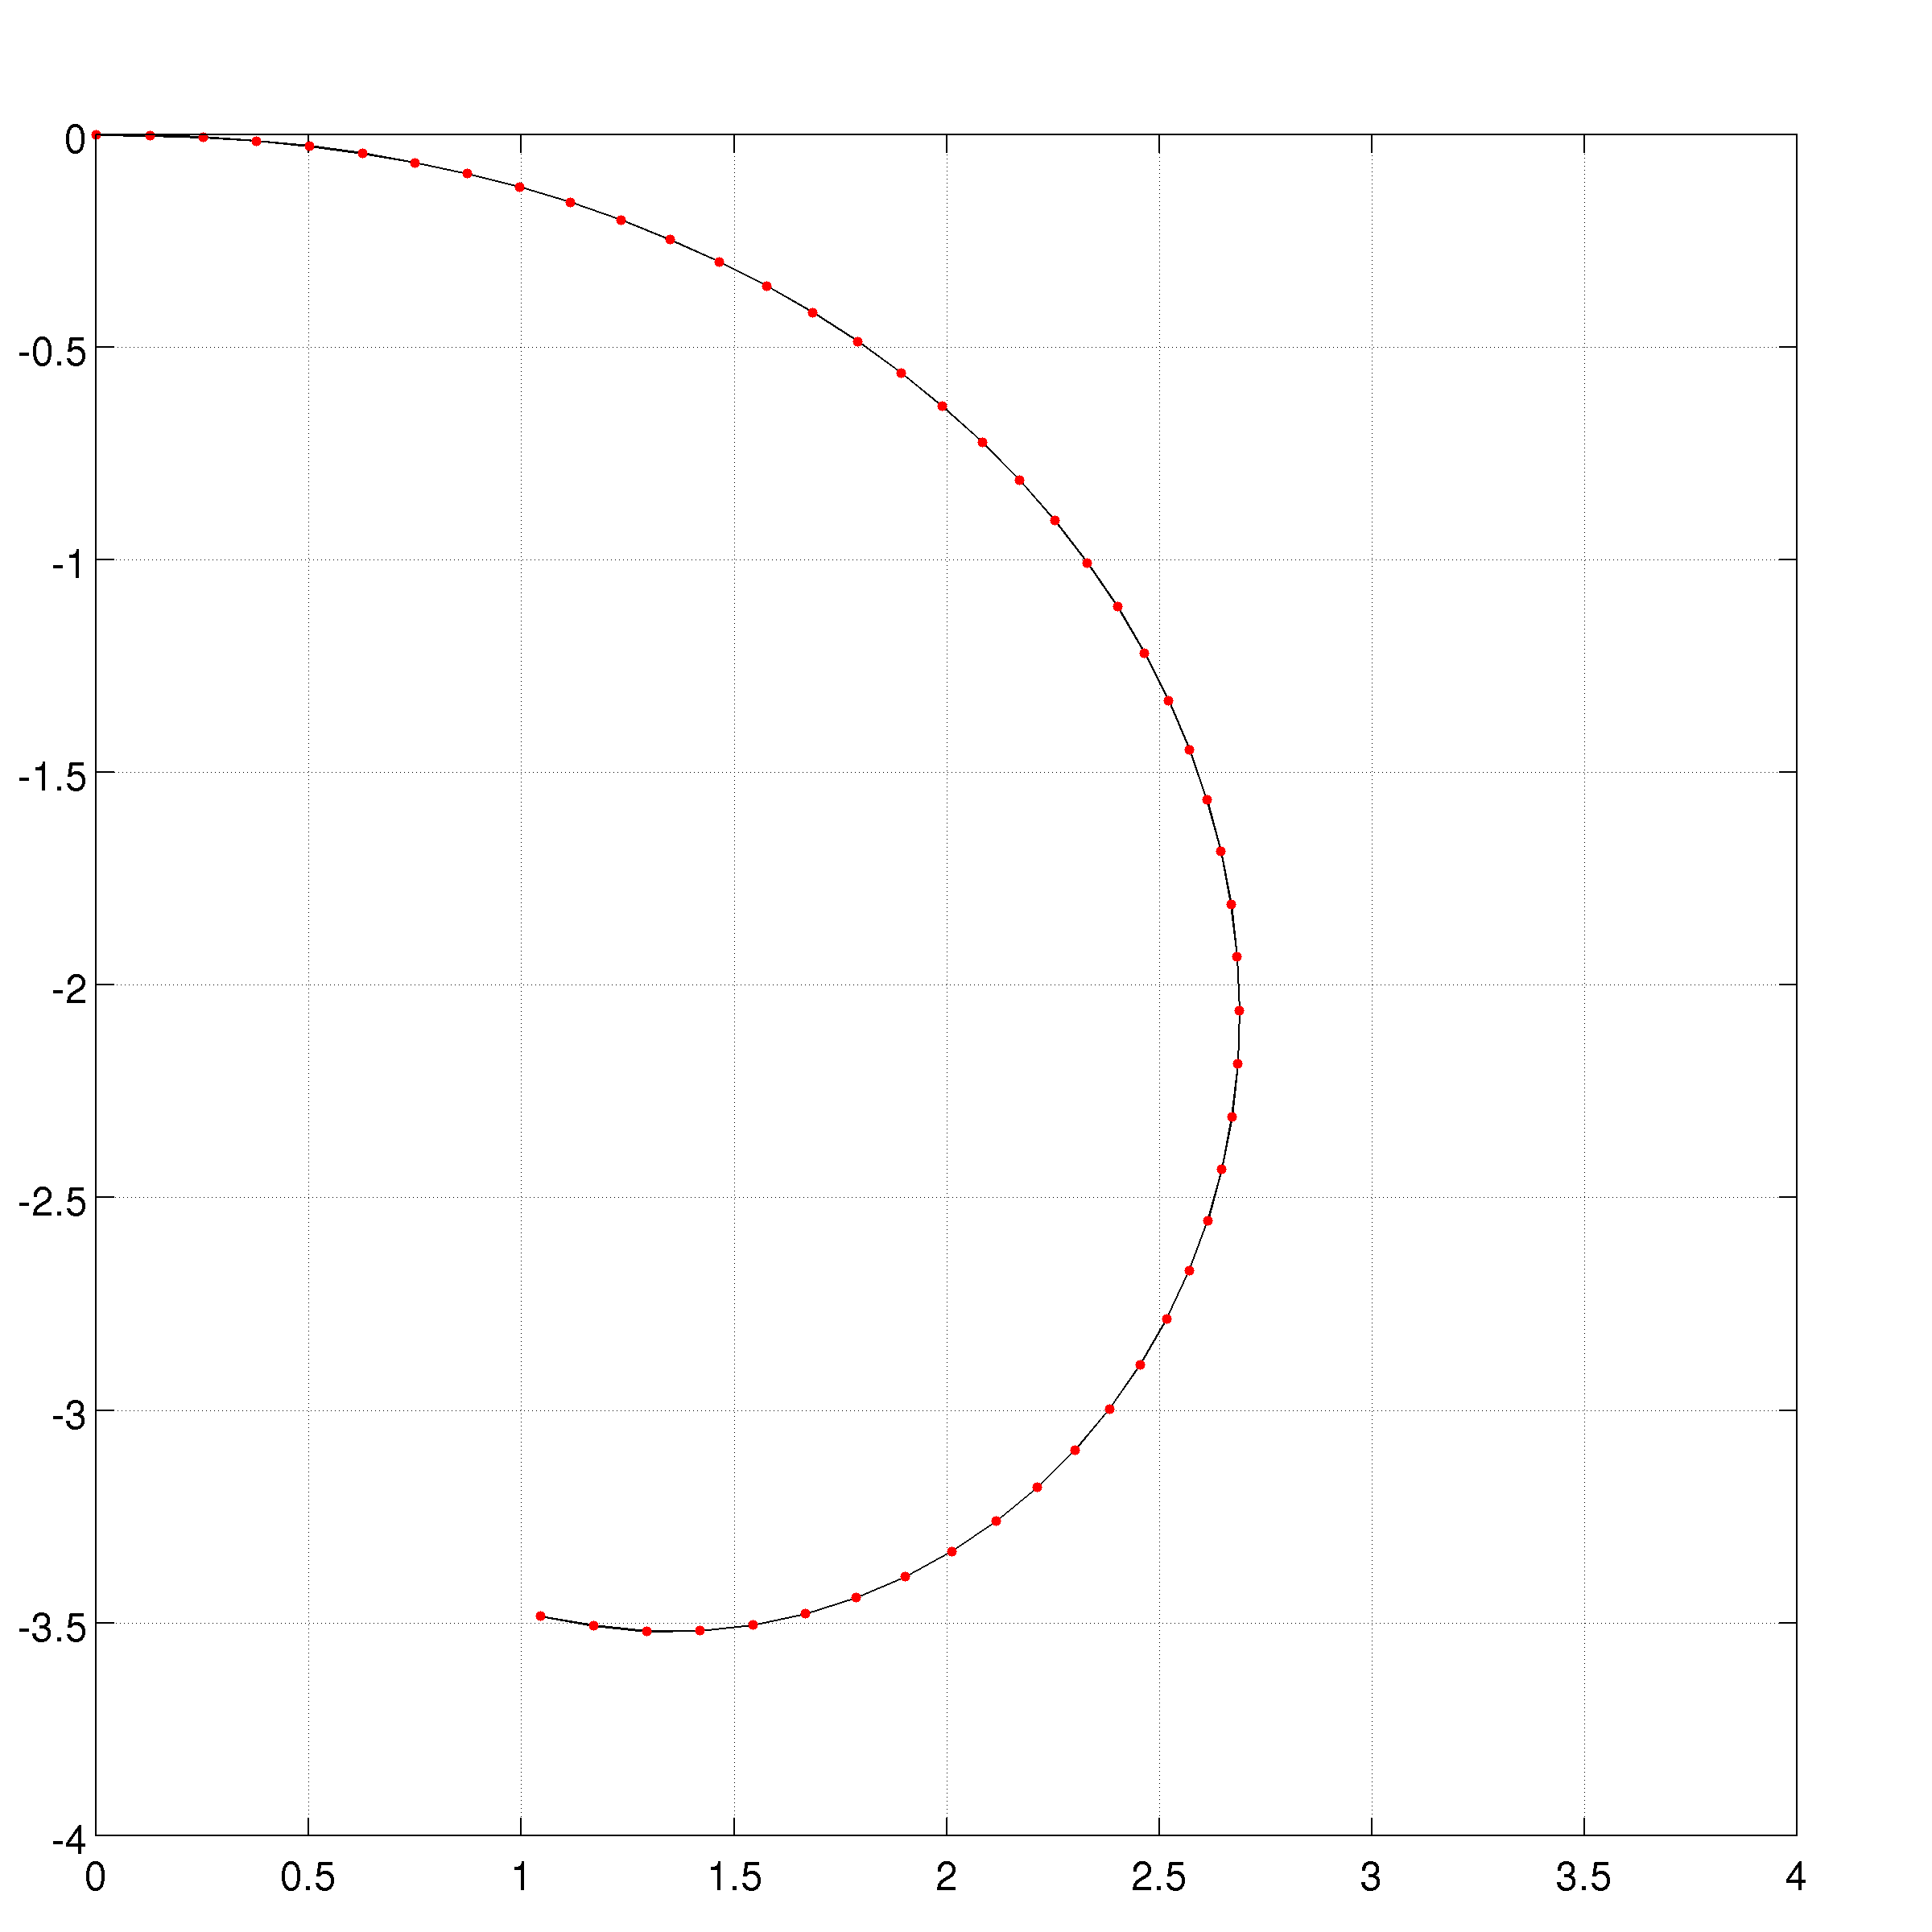
\includegraphics[width=\anchoseis]{\chapFiveDir/results/curvature/example_01/ani_curve_0.90.png}\\
	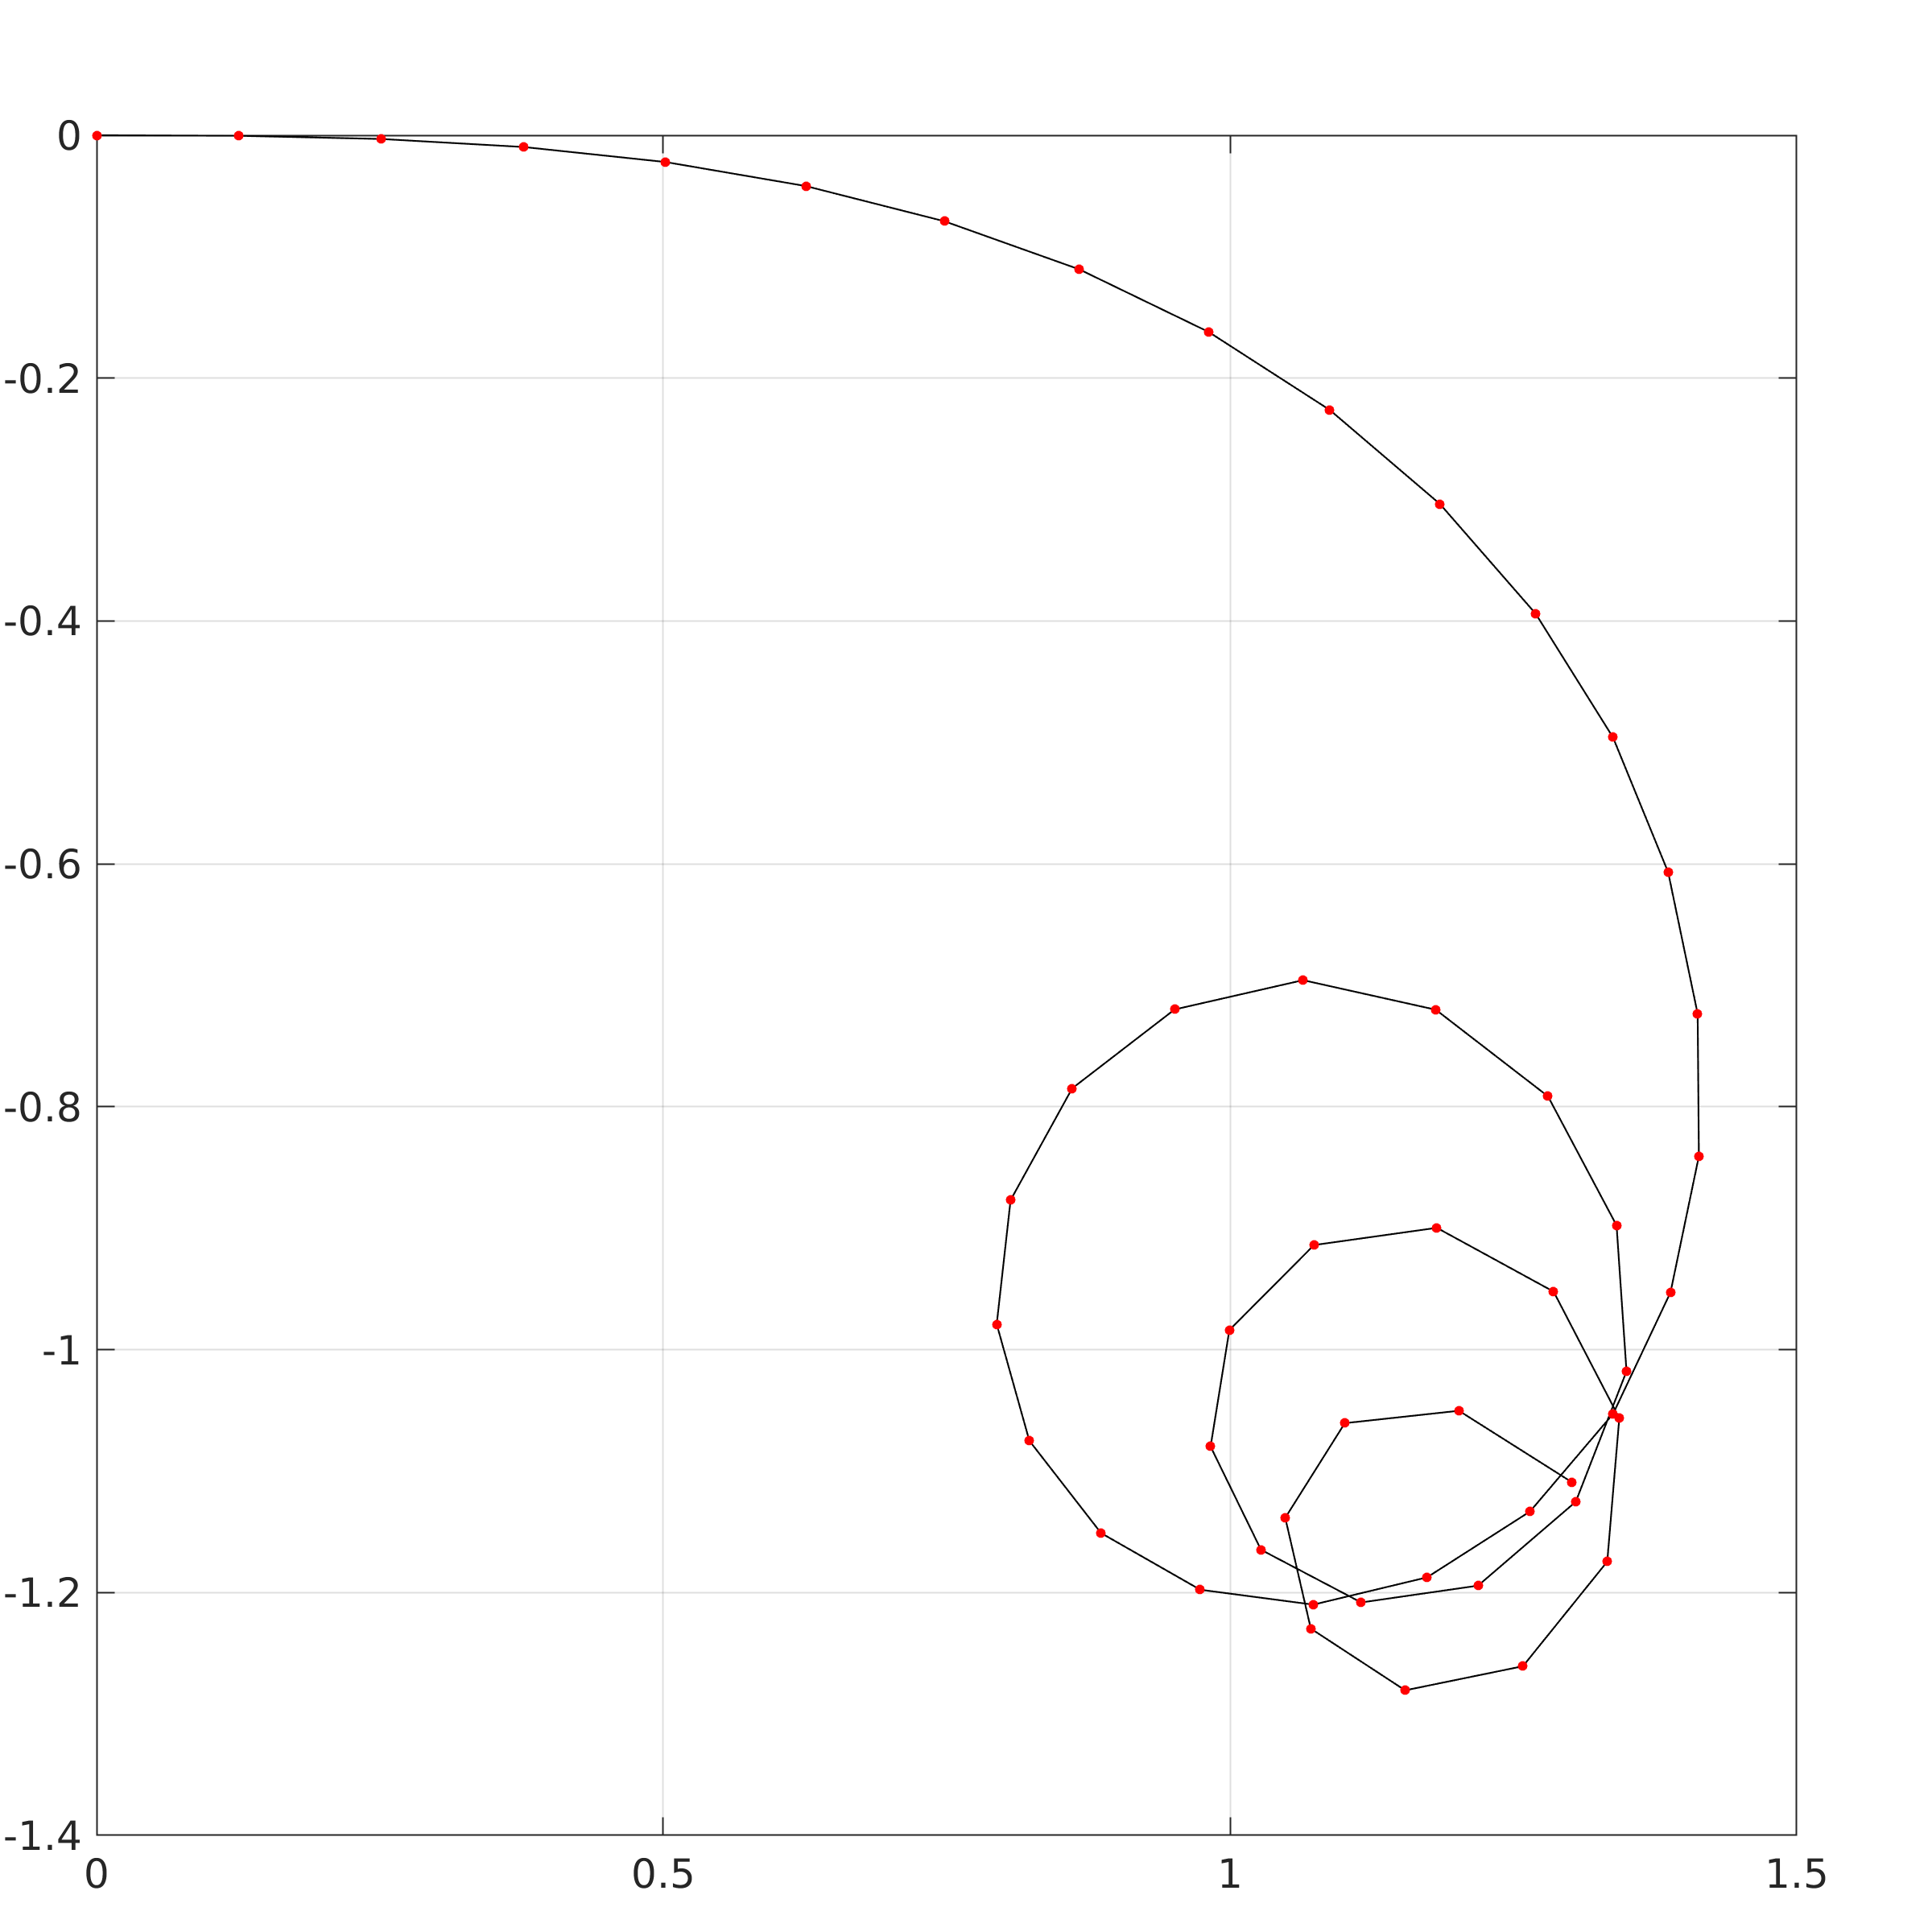
\includegraphics[width=\anchoseis]{\chapFiveDir/results/euclidean/example_01/ani_euc_0.10.png}
	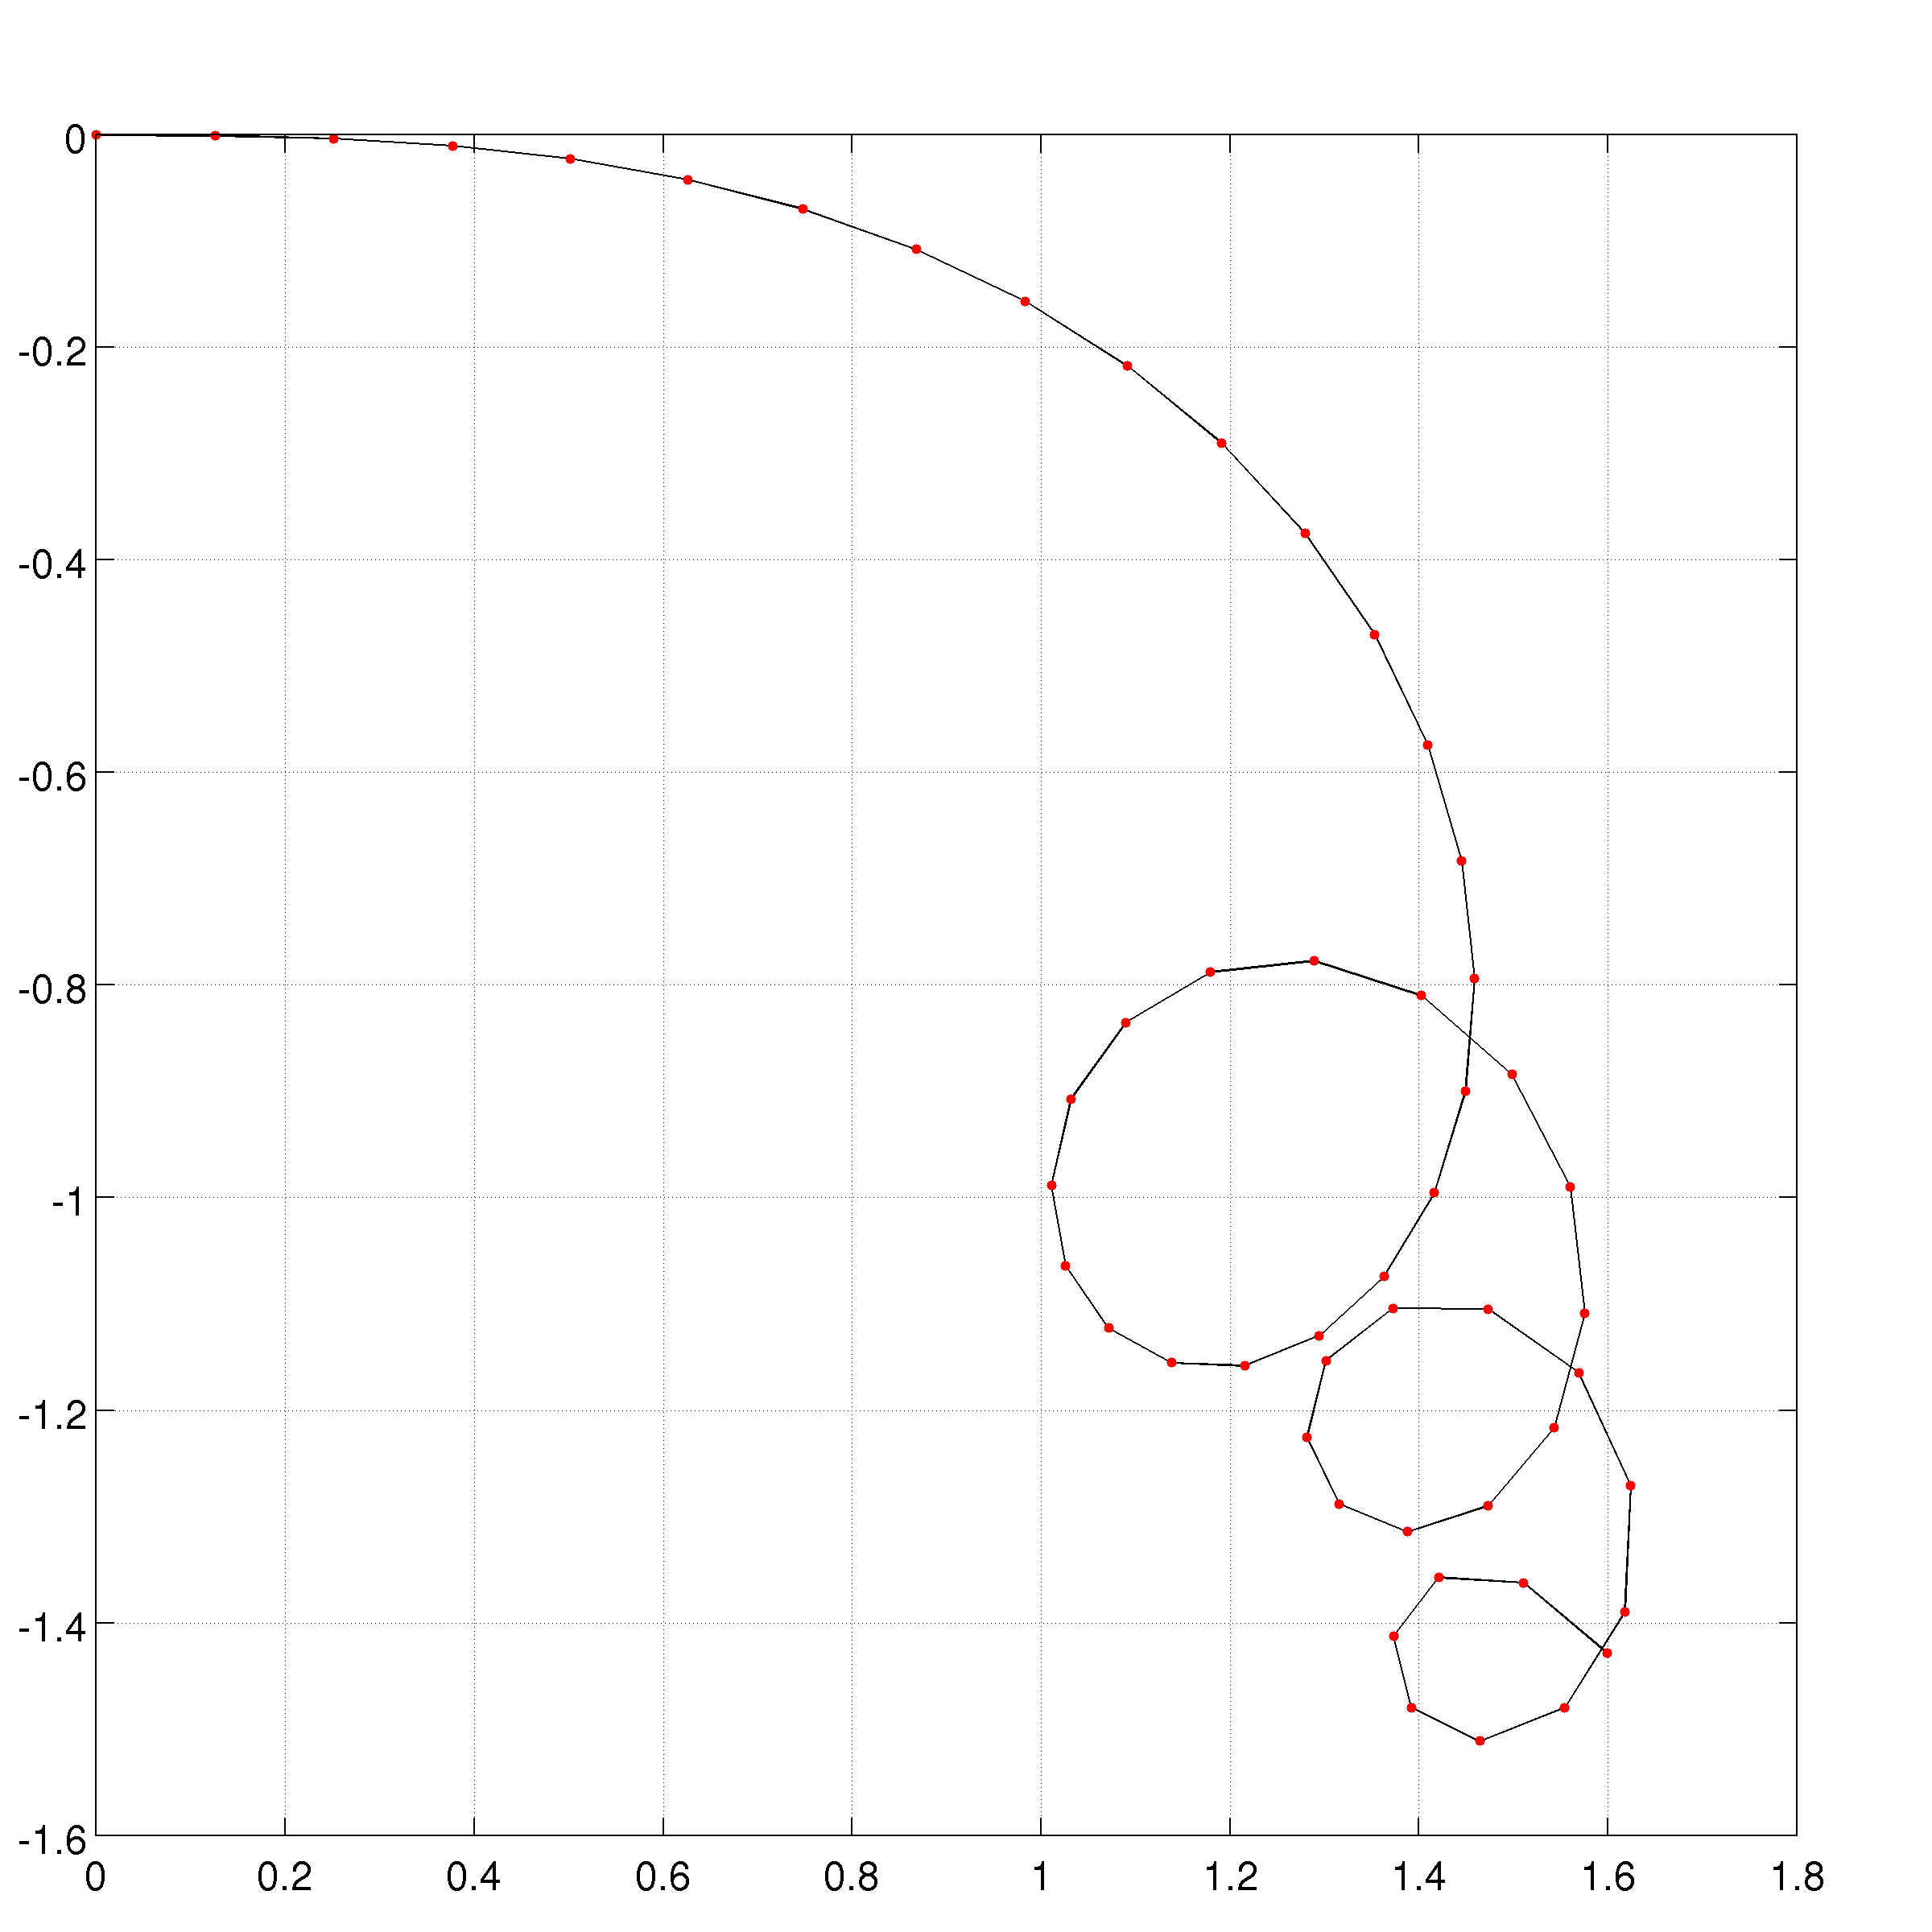
\includegraphics[width=\anchoseis]{\chapFiveDir/results/euclidean/example_01/ani_euc_0.20.png}
	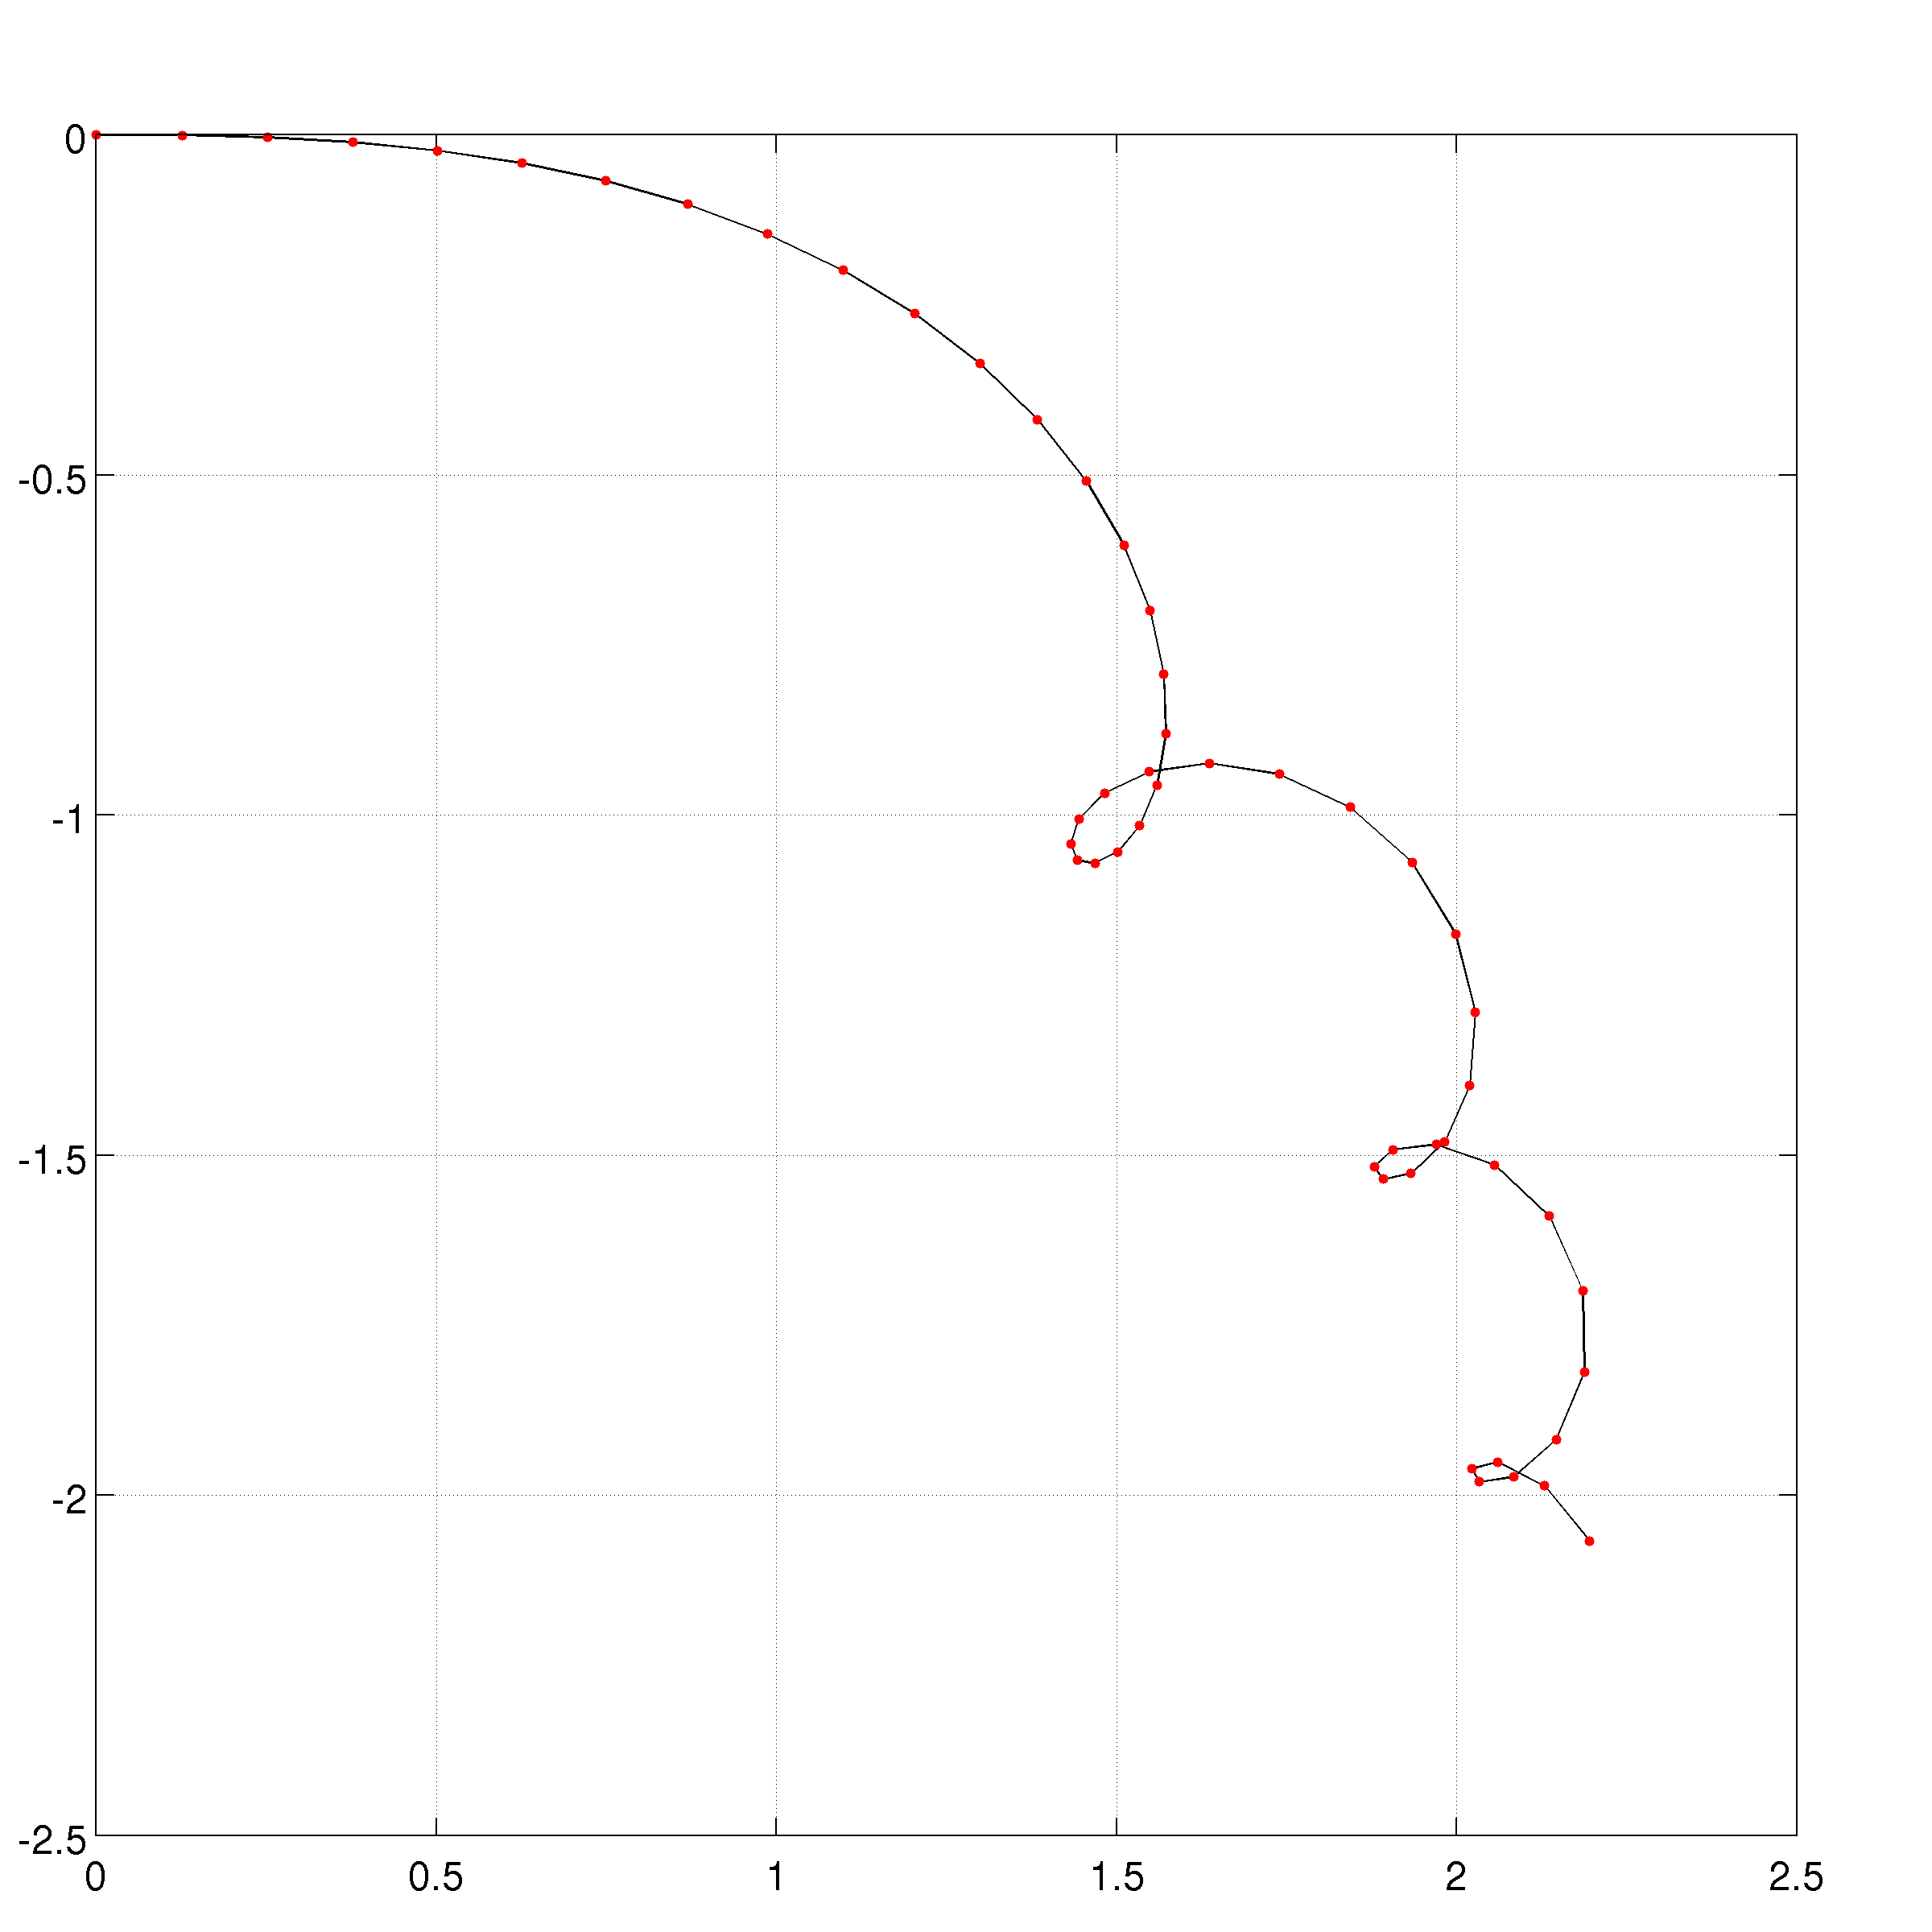
\includegraphics[width=\anchoseis]{\chapFiveDir/results/euclidean/example_01/ani_euc_0.40.png}
	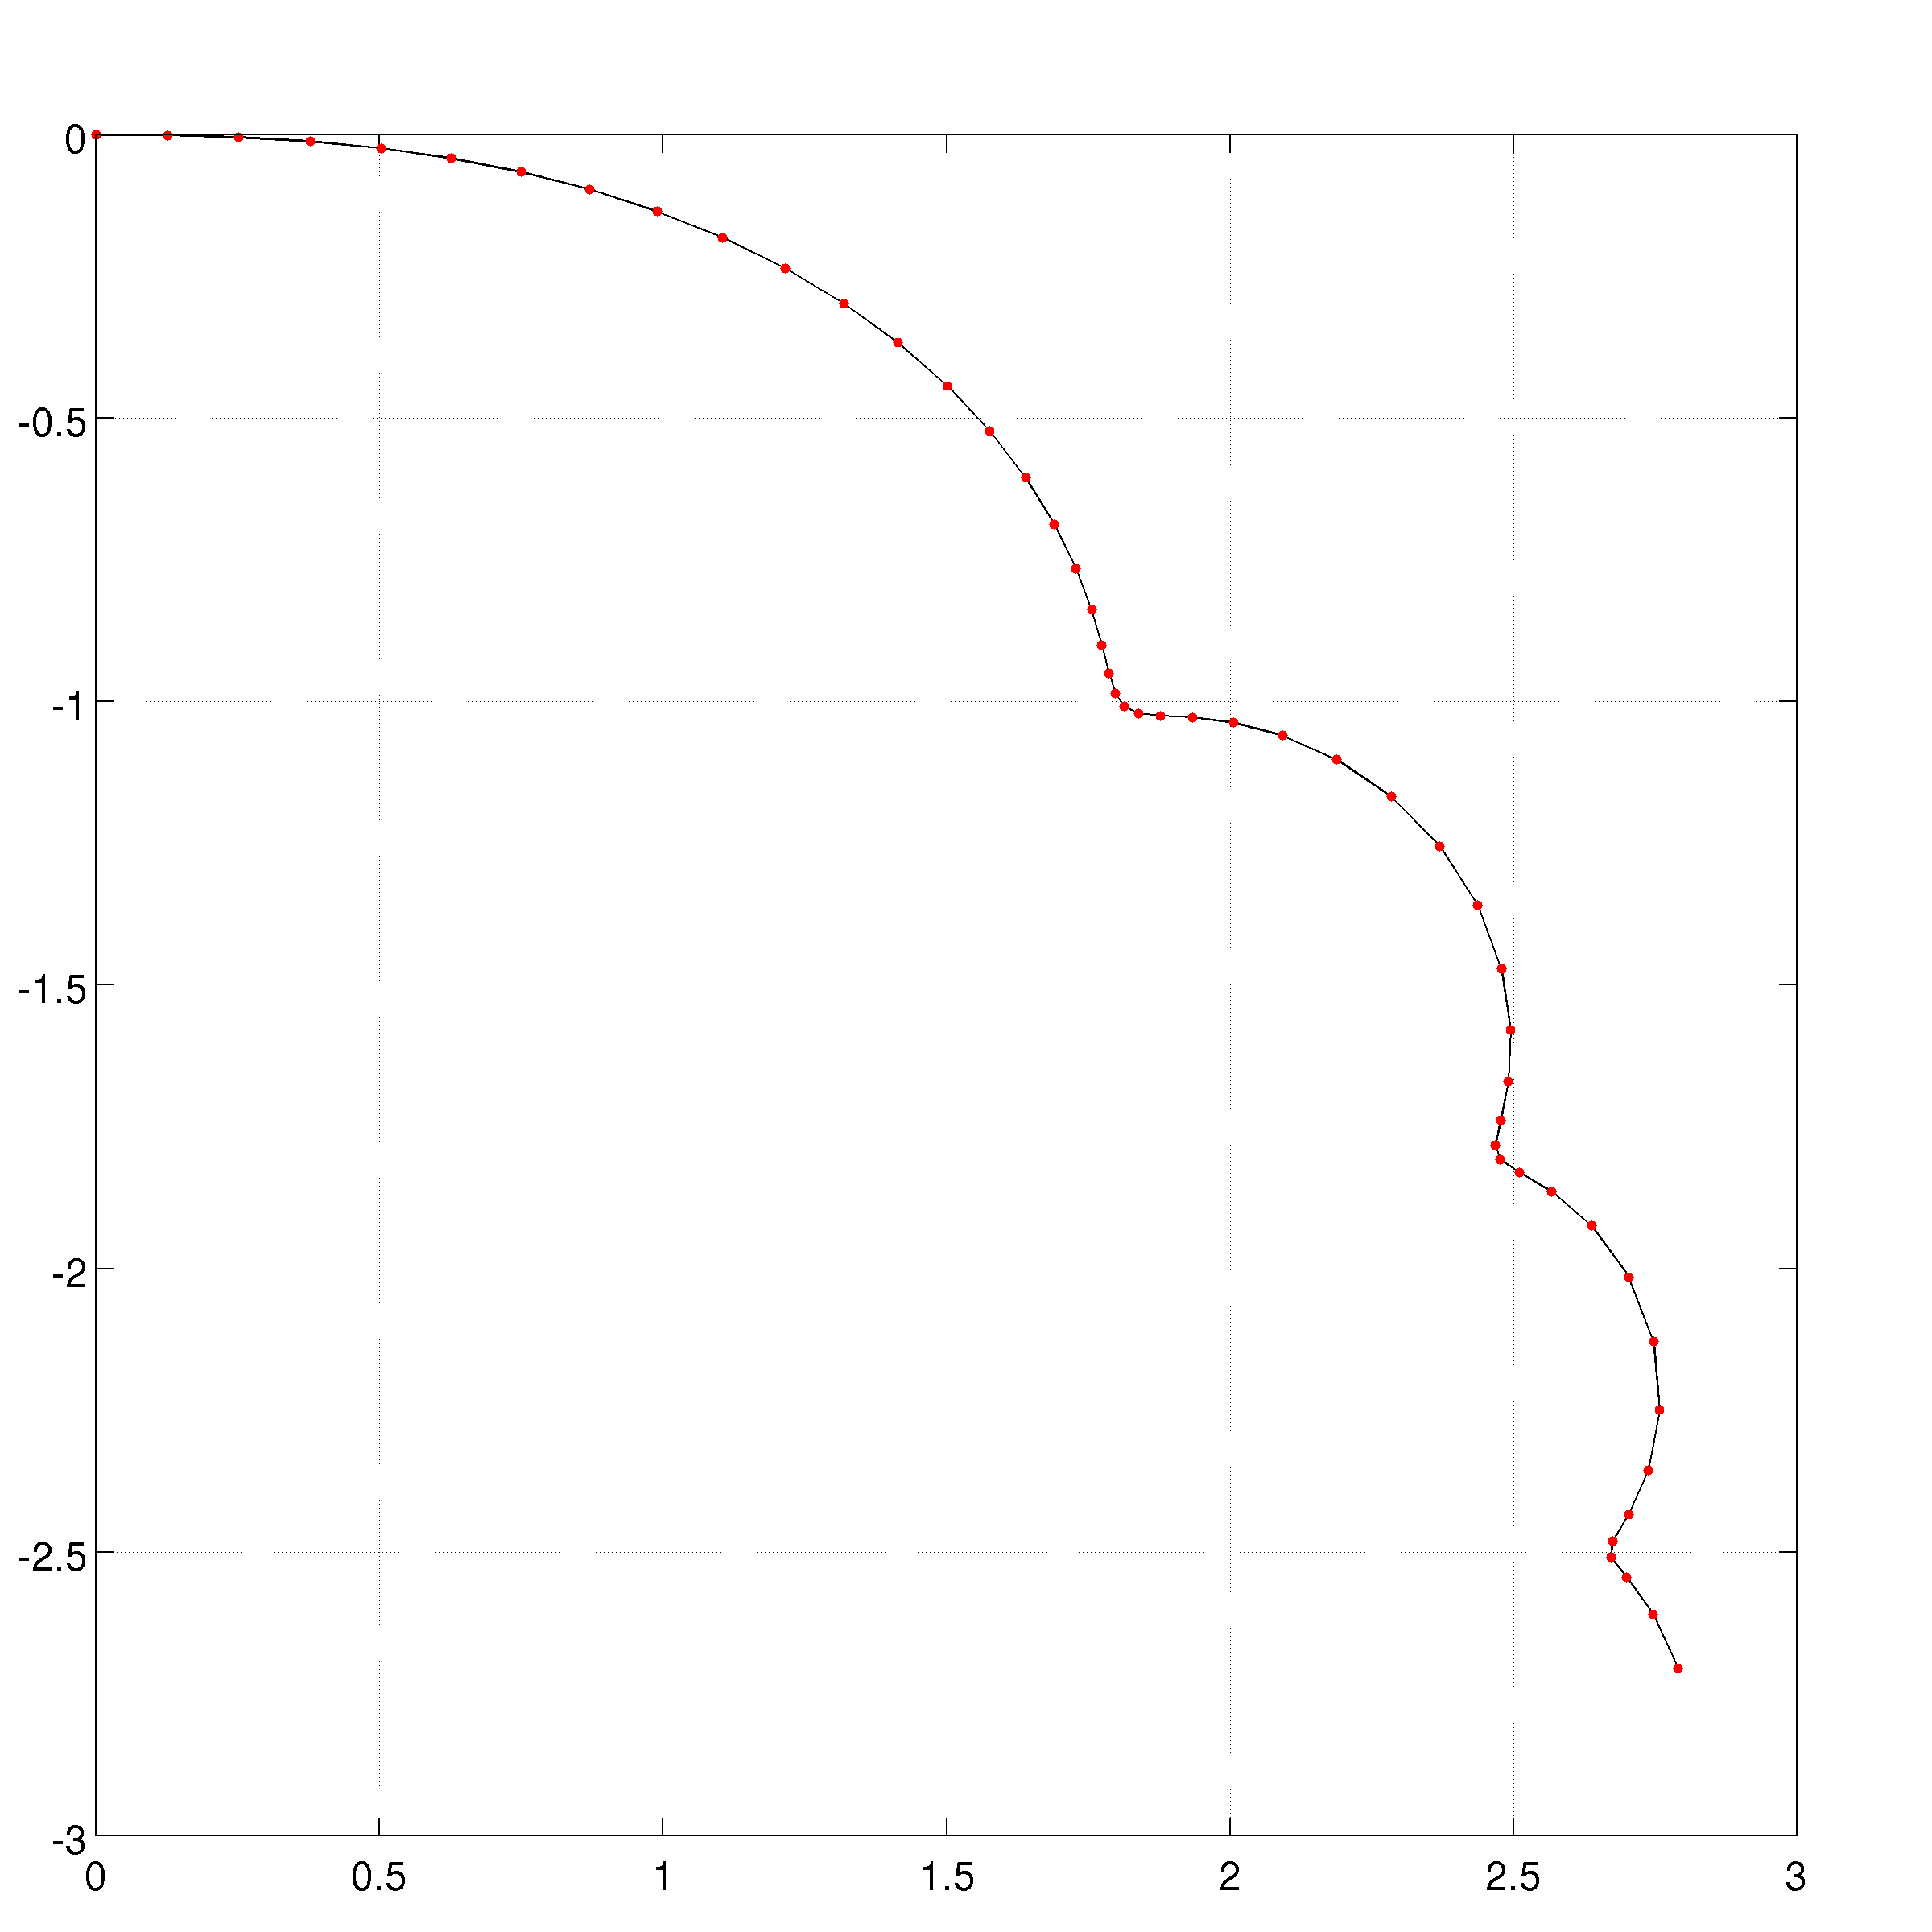
\includegraphics[width=\anchoseis]{\chapFiveDir/results/euclidean/example_01/ani_euc_0.60.png}
	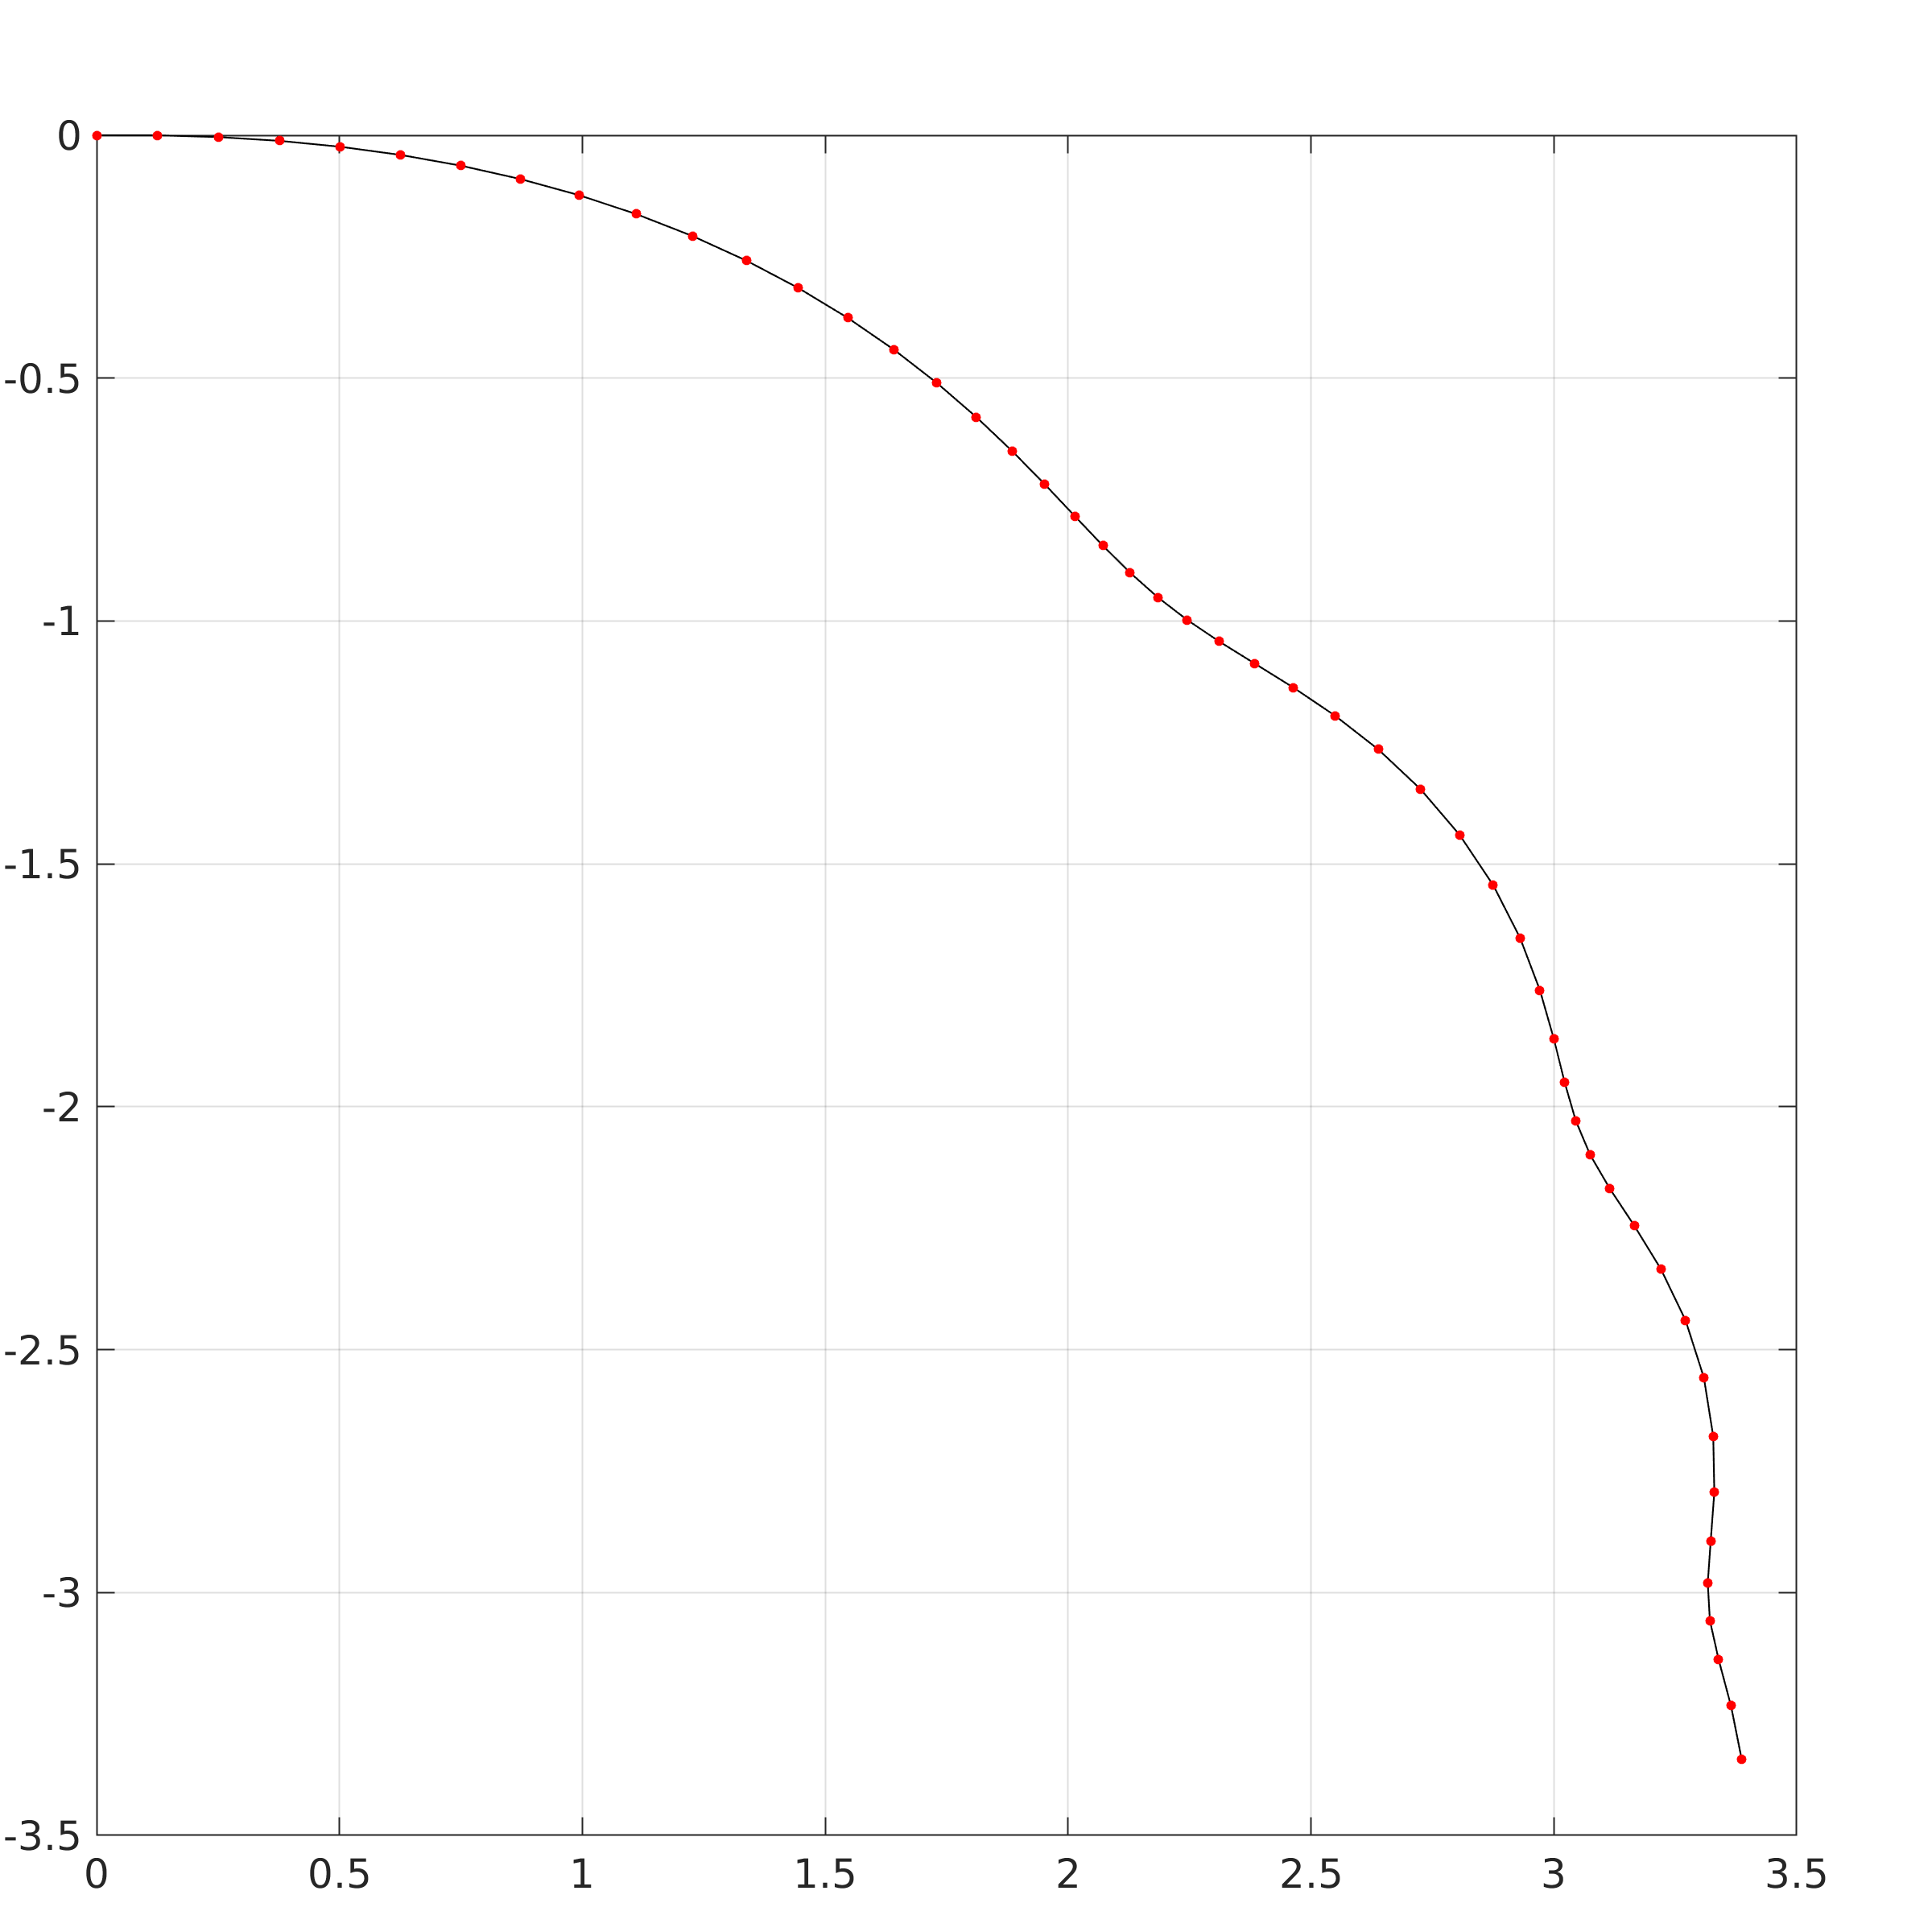
\includegraphics[width=\anchoseis]{\chapFiveDir/results/euclidean/example_01/ani_euc_0.80.png}
	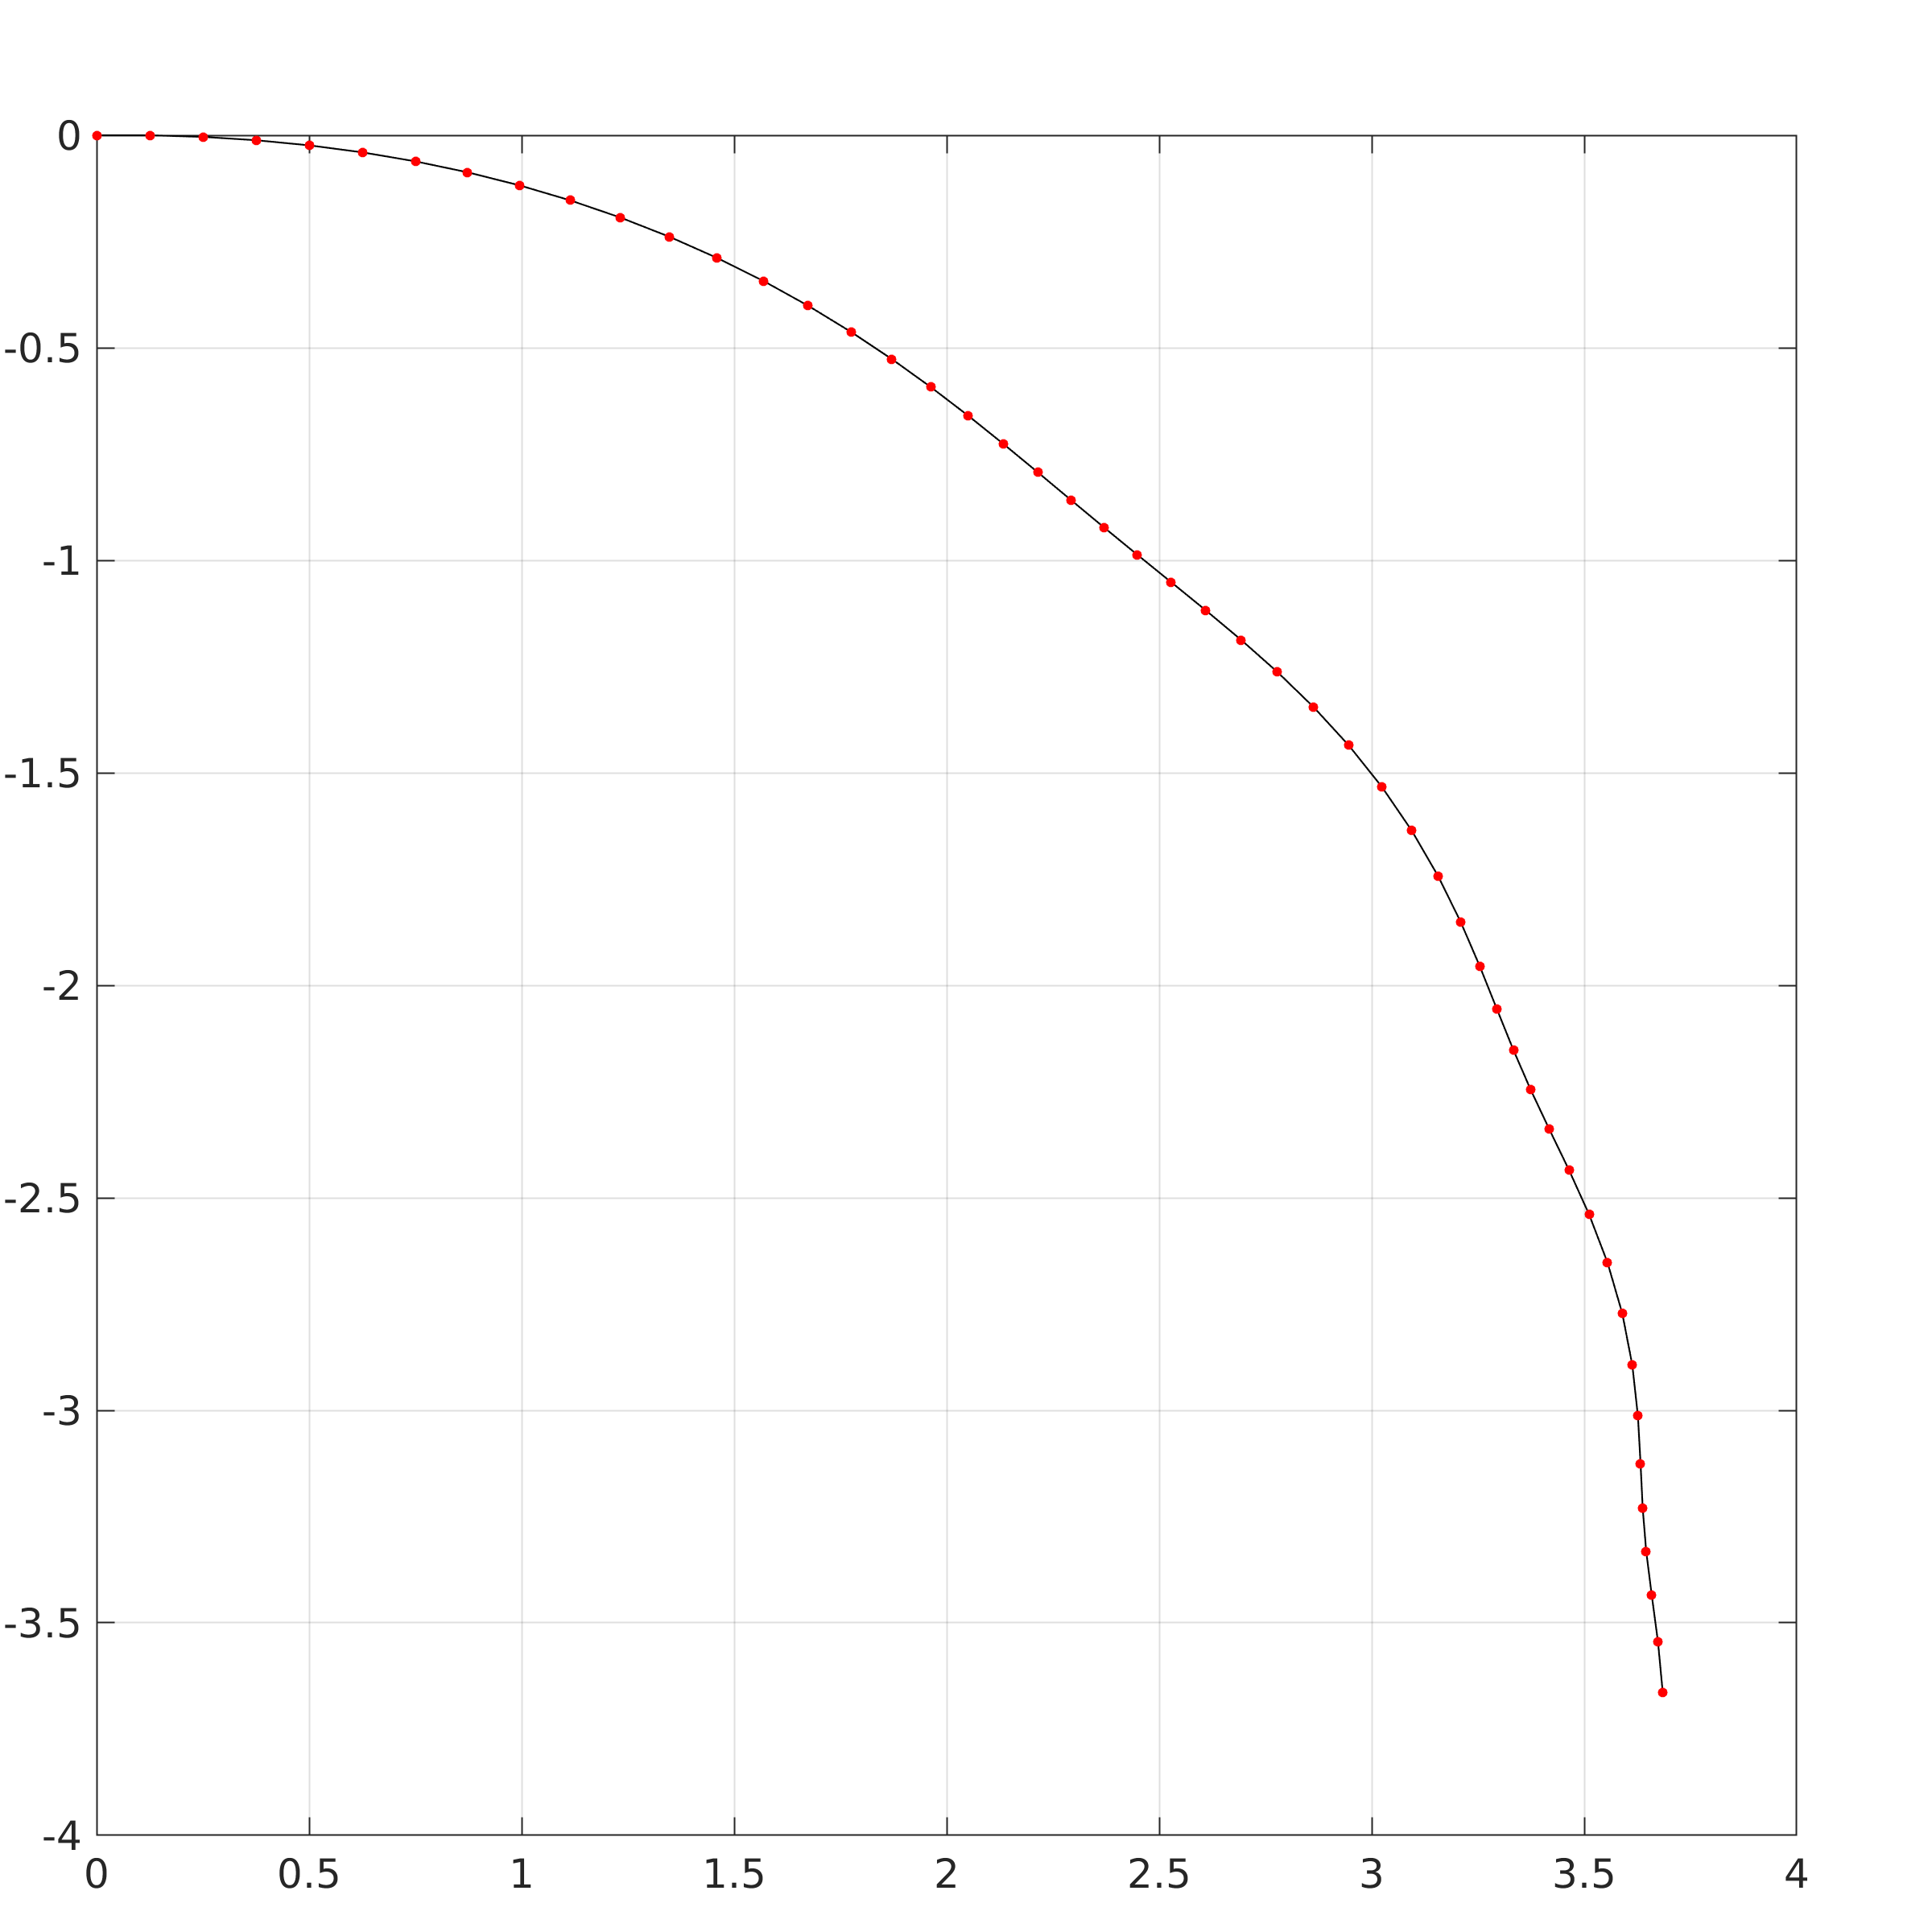
\includegraphics[width=\anchoseis]{\chapFiveDir/results/euclidean/example_01/ani_euc_0.90.png}
	\caption{Example 1: Comparison between Euclidean and Curvature interpolation at intermediate times \mbox{[0.1 0.2 0.4 0.6 0.8 0.9]}. Top: Curvature interpolation. Bottom: Euclidean interpolation.}
	\label{fig:curve_interpolation:results:parametric:animation}
\end{figure}	


In the second example, we interpolate two hand drawn U-letters, as shown in Figure \ref{fig:curve_interpolation:results:letter_u:input}. Both curves have a very sparse and irregular sampling, with a different number of control points. As we explained before, both curves are interpolated to obtain a dense, regular and constant speed sampling.

\begin{figure}[h]
	\centering
		\subfloat[]{
		\includegraphics[width=\anchodos]{\chapFiveDir/curves/letter_u/c1.png}
		\label{fig:curve_interpolation:results:letter_u:input:c1}
	}
	\subfloat[]{
		\includegraphics[width=\anchodos]{\chapFiveDir/curves/letter_u/c2.png}
		\label{fig:curve_interpolation:results:letter_u:input:c2}
	}
	\caption{Example 2: Input curves expressed as control points. The objective is to interpolate two hand written U-letters. The first letter shown in \protect\subref{fig:curve_interpolation:results:letter_u:input:c1} is bigger and has different concavities on the sides of the shape than the second letter shown in \protect\subref{fig:curve_interpolation:results:letter_u:input:c2}. They also have a different number of control points. }
	\label{fig:curve_interpolation:results:letter_u:input}
\end{figure}	

In Figure \ref{fig:curve_interpolation:results:letter_u:output} we depict the process of interpolation. First, in Figure \ref{fig:curve_interpolation:results:letter_u:output:transform_only}, we interpolate the intrinsic description of the curves and obtain a resulting curve which has a correct shape but wrong placement. Using the mid point of the curve and the initial angle, we estimate the intermediate position and orientation and apply it to the curve, as shown in Figure \ref{fig:curve_interpolation:results:letter_u:output:transform_and_rigid}, and it ends at the correct position.

\begin{figure}[h]
	\centering
		\subfloat[]{
		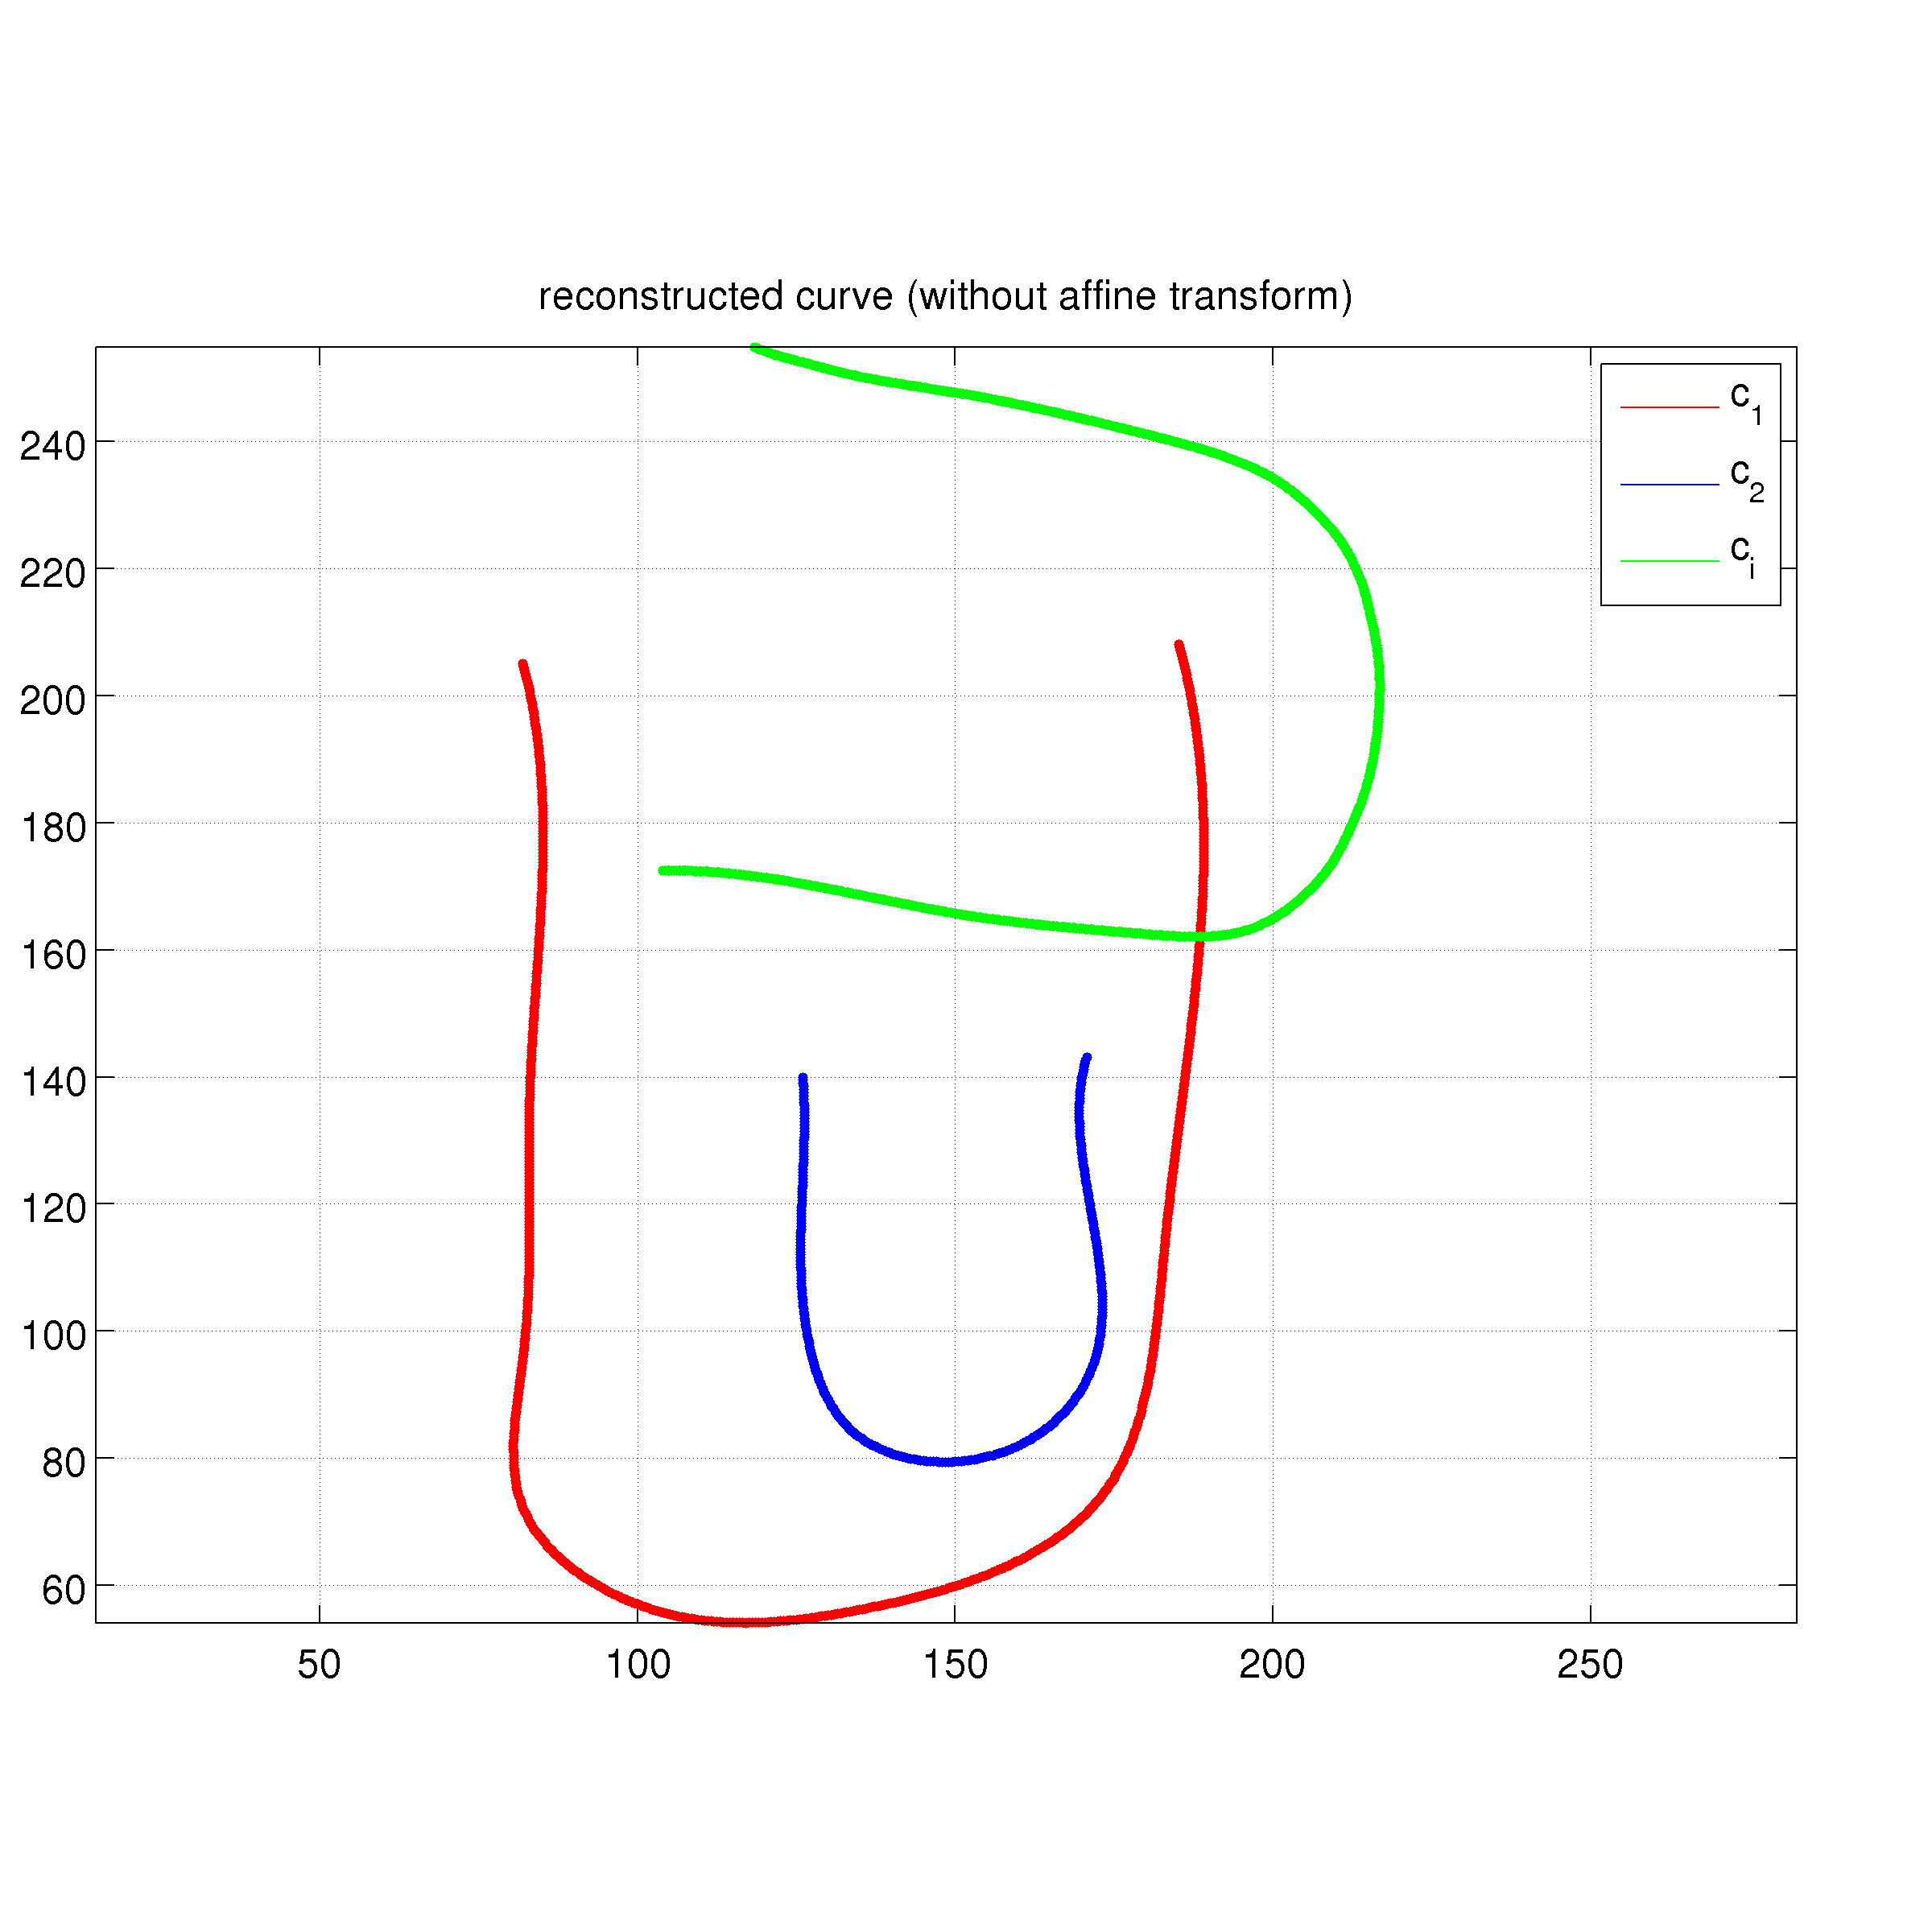
\includegraphics[width=\anchodos]{\chapFiveDir/curves/letter_u/curvature_reconstructed_without_transform}
		\label{fig:curve_interpolation:results:letter_u:output:transform_only}
	}
	\subfloat[]{
		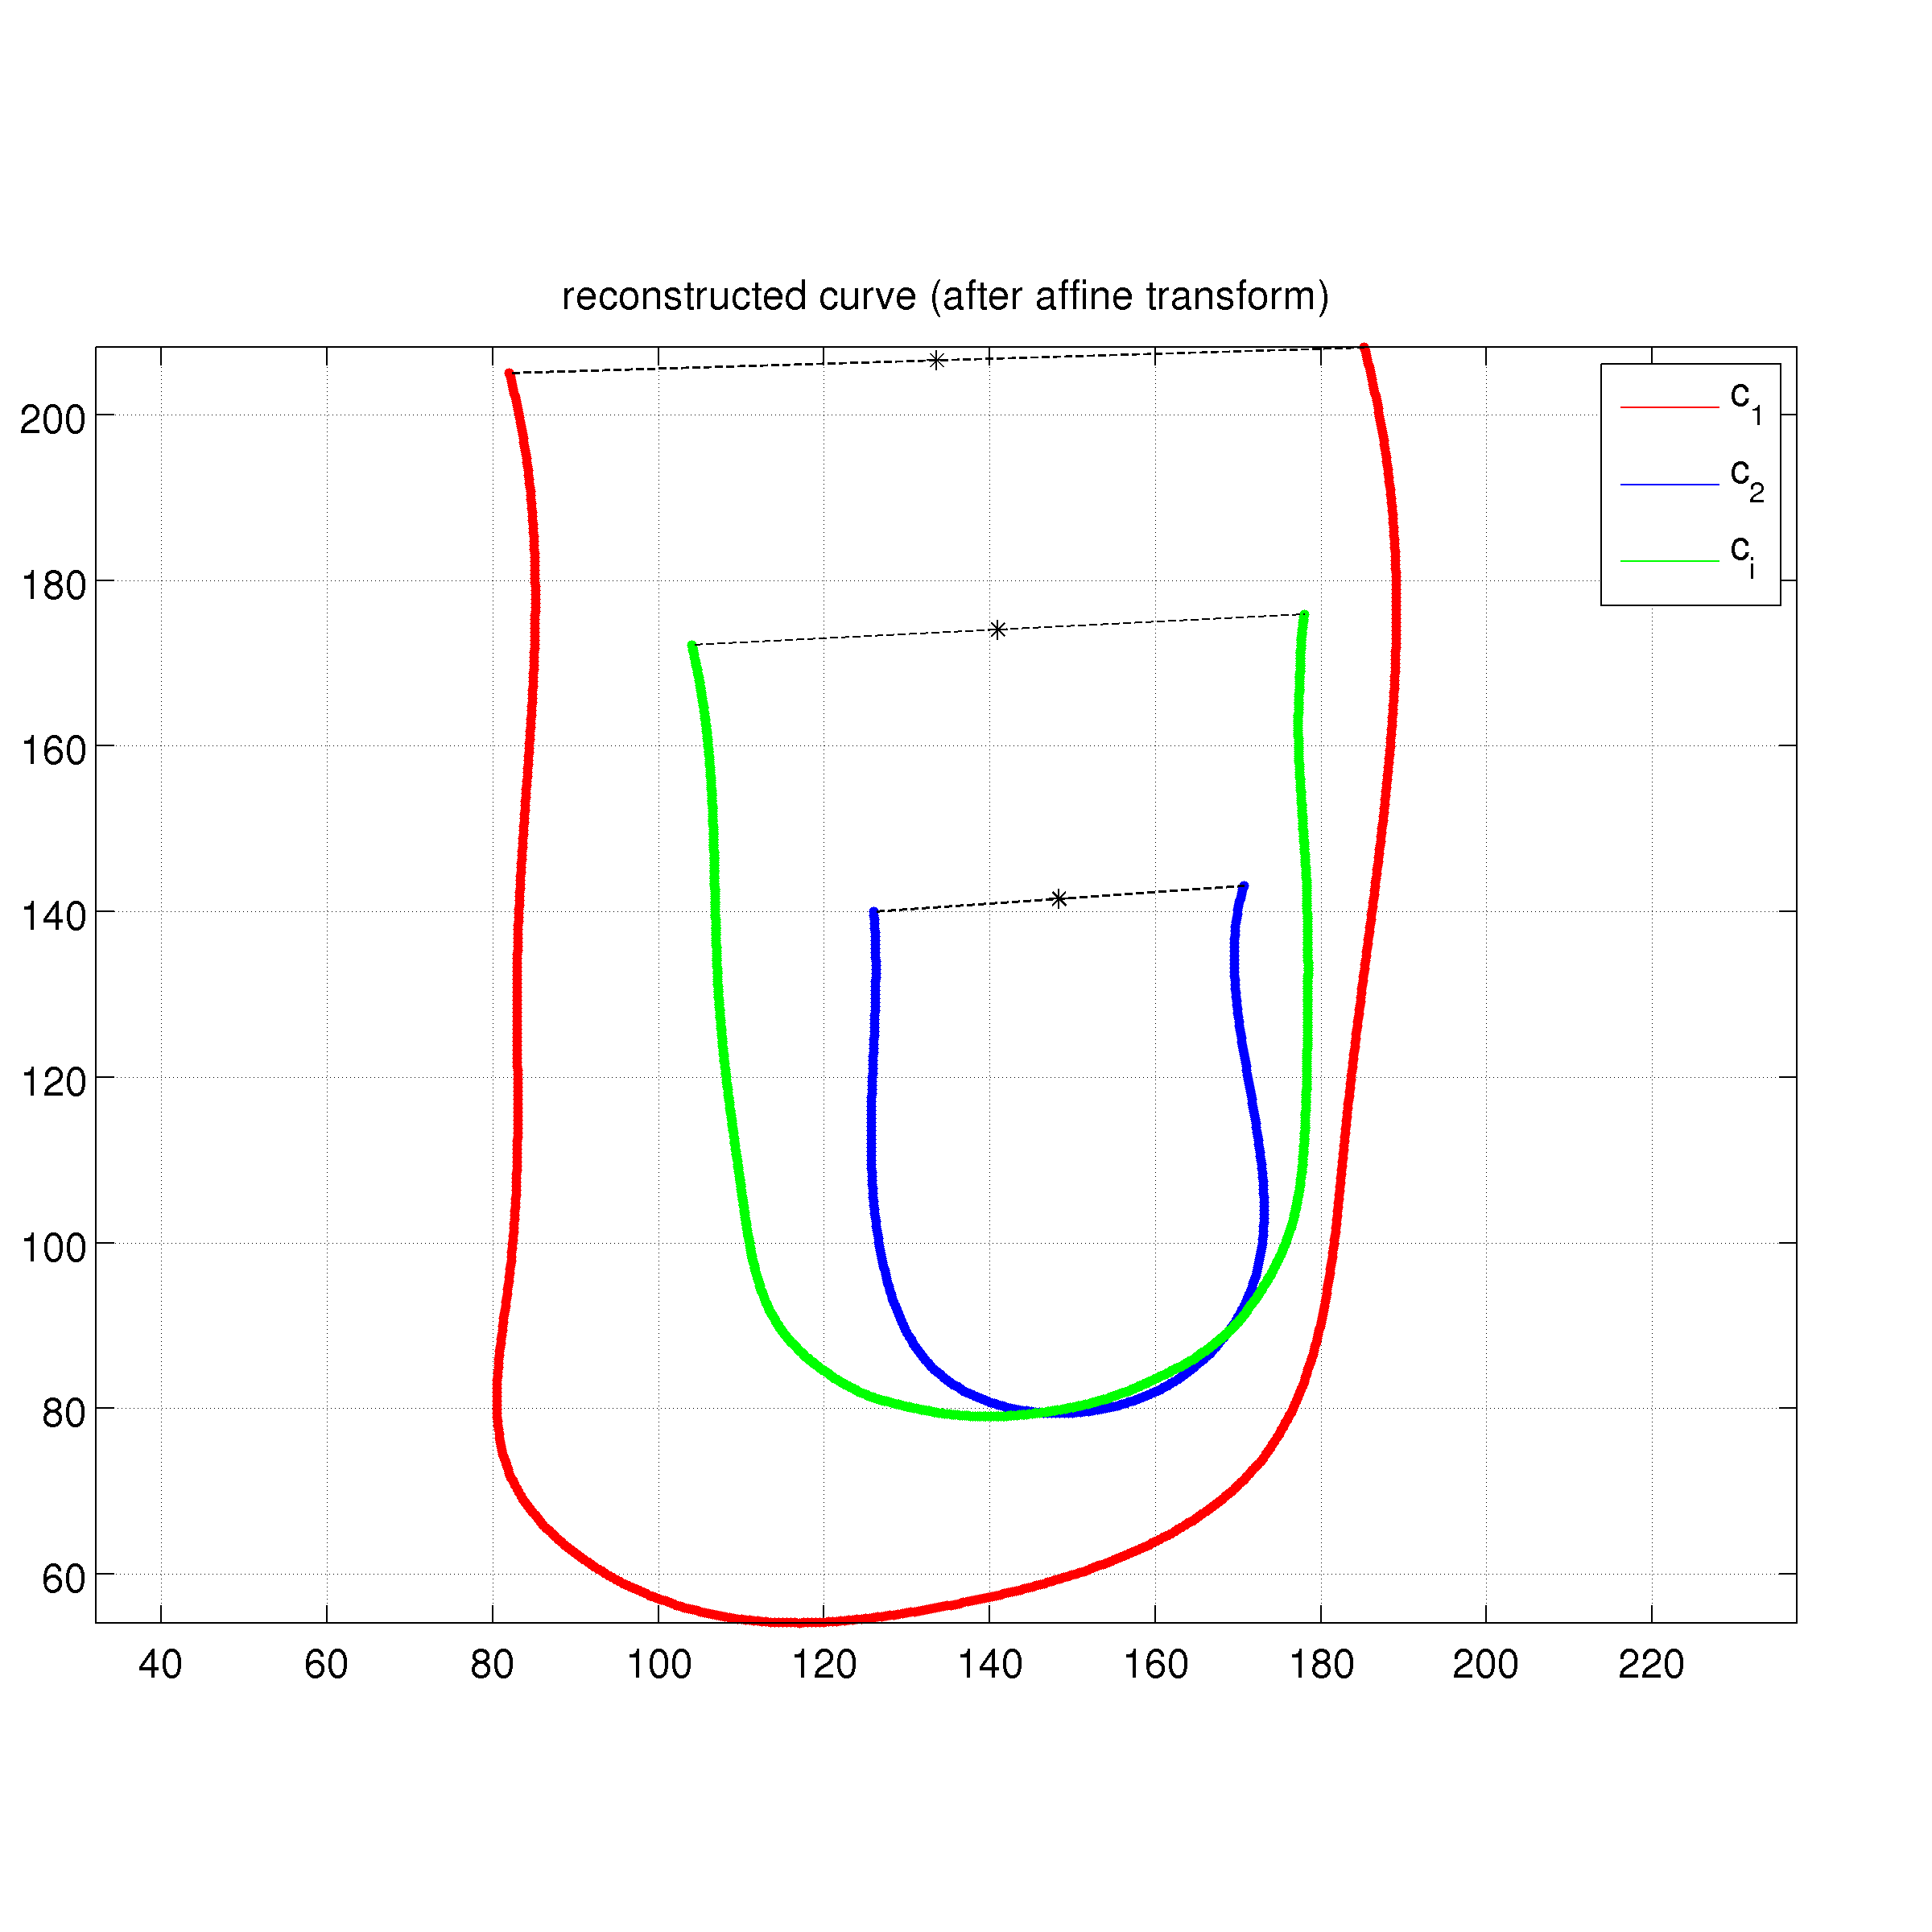
\includegraphics[width=\anchodos]{\chapFiveDir/curves/letter_u/curvature_reconstructed_with_transform}
		\label{fig:curve_interpolation:results:letter_u:output:transform_and_rigid}
	}
	\caption{
		Example 2: Results of interpolating the U shaped letters from Figure \ref{fig:curve_interpolation:results:letter_u:input}. In red we show the first (and bigger) U-letter, in blue the second (and smaller) U-letter, and in green the resulting interpolation.
		\protect\subref{fig:curve_interpolation:results:letter_u:output:transform_only} When we use only the curvature signatures we can see that the resulting curve has a correct shape but the location and rotation are off.
		\protect\subref{fig:curve_interpolation:results:letter_u:output:transform_and_rigid} If we add angle and position interpolation, we can see that the curve gets better positioned.
	}
	\label{fig:curve_interpolation:results:letter_u:output}
\end{figure}	

Finally, in Figure \ref{fig:curve_interpolation:results:letter_u:animation} we describe the intermediate steps in the interpolation between both letters.

\begin{figure}[h]
	\centering
	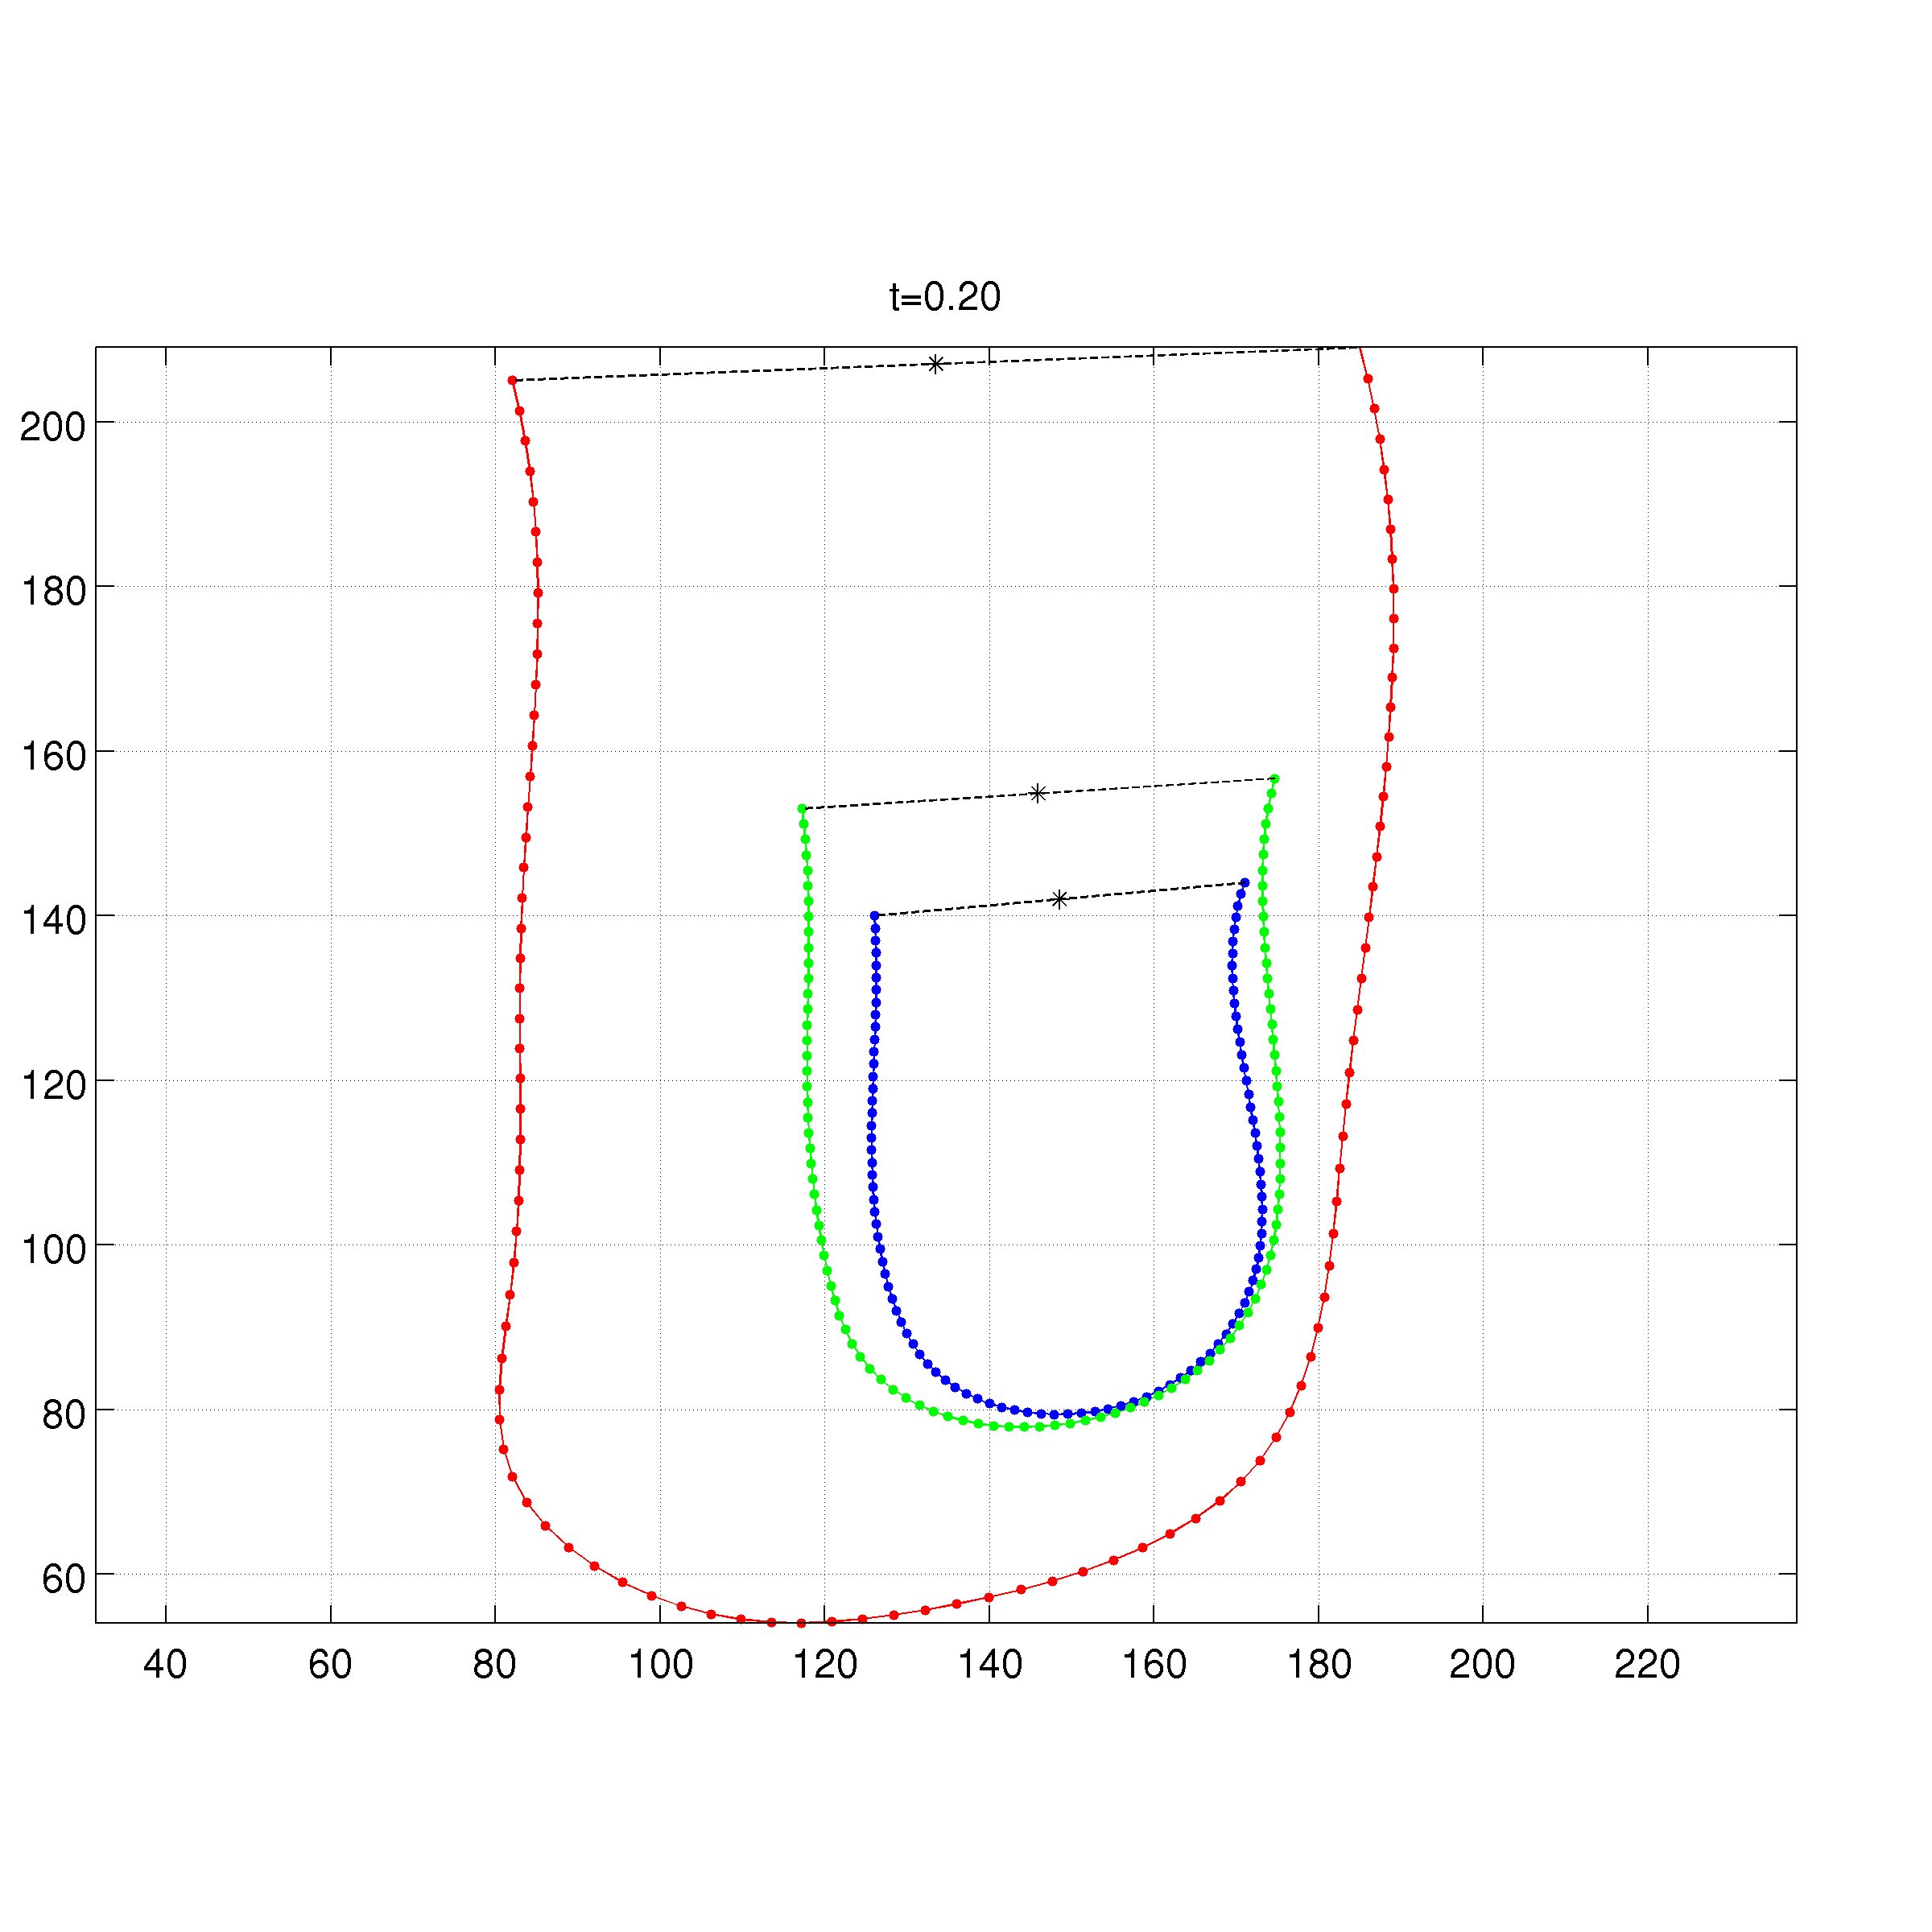
\includegraphics[width=\anchocuatro]{\chapFiveDir/curves/letter_u/animation/interp_0.20.png}
	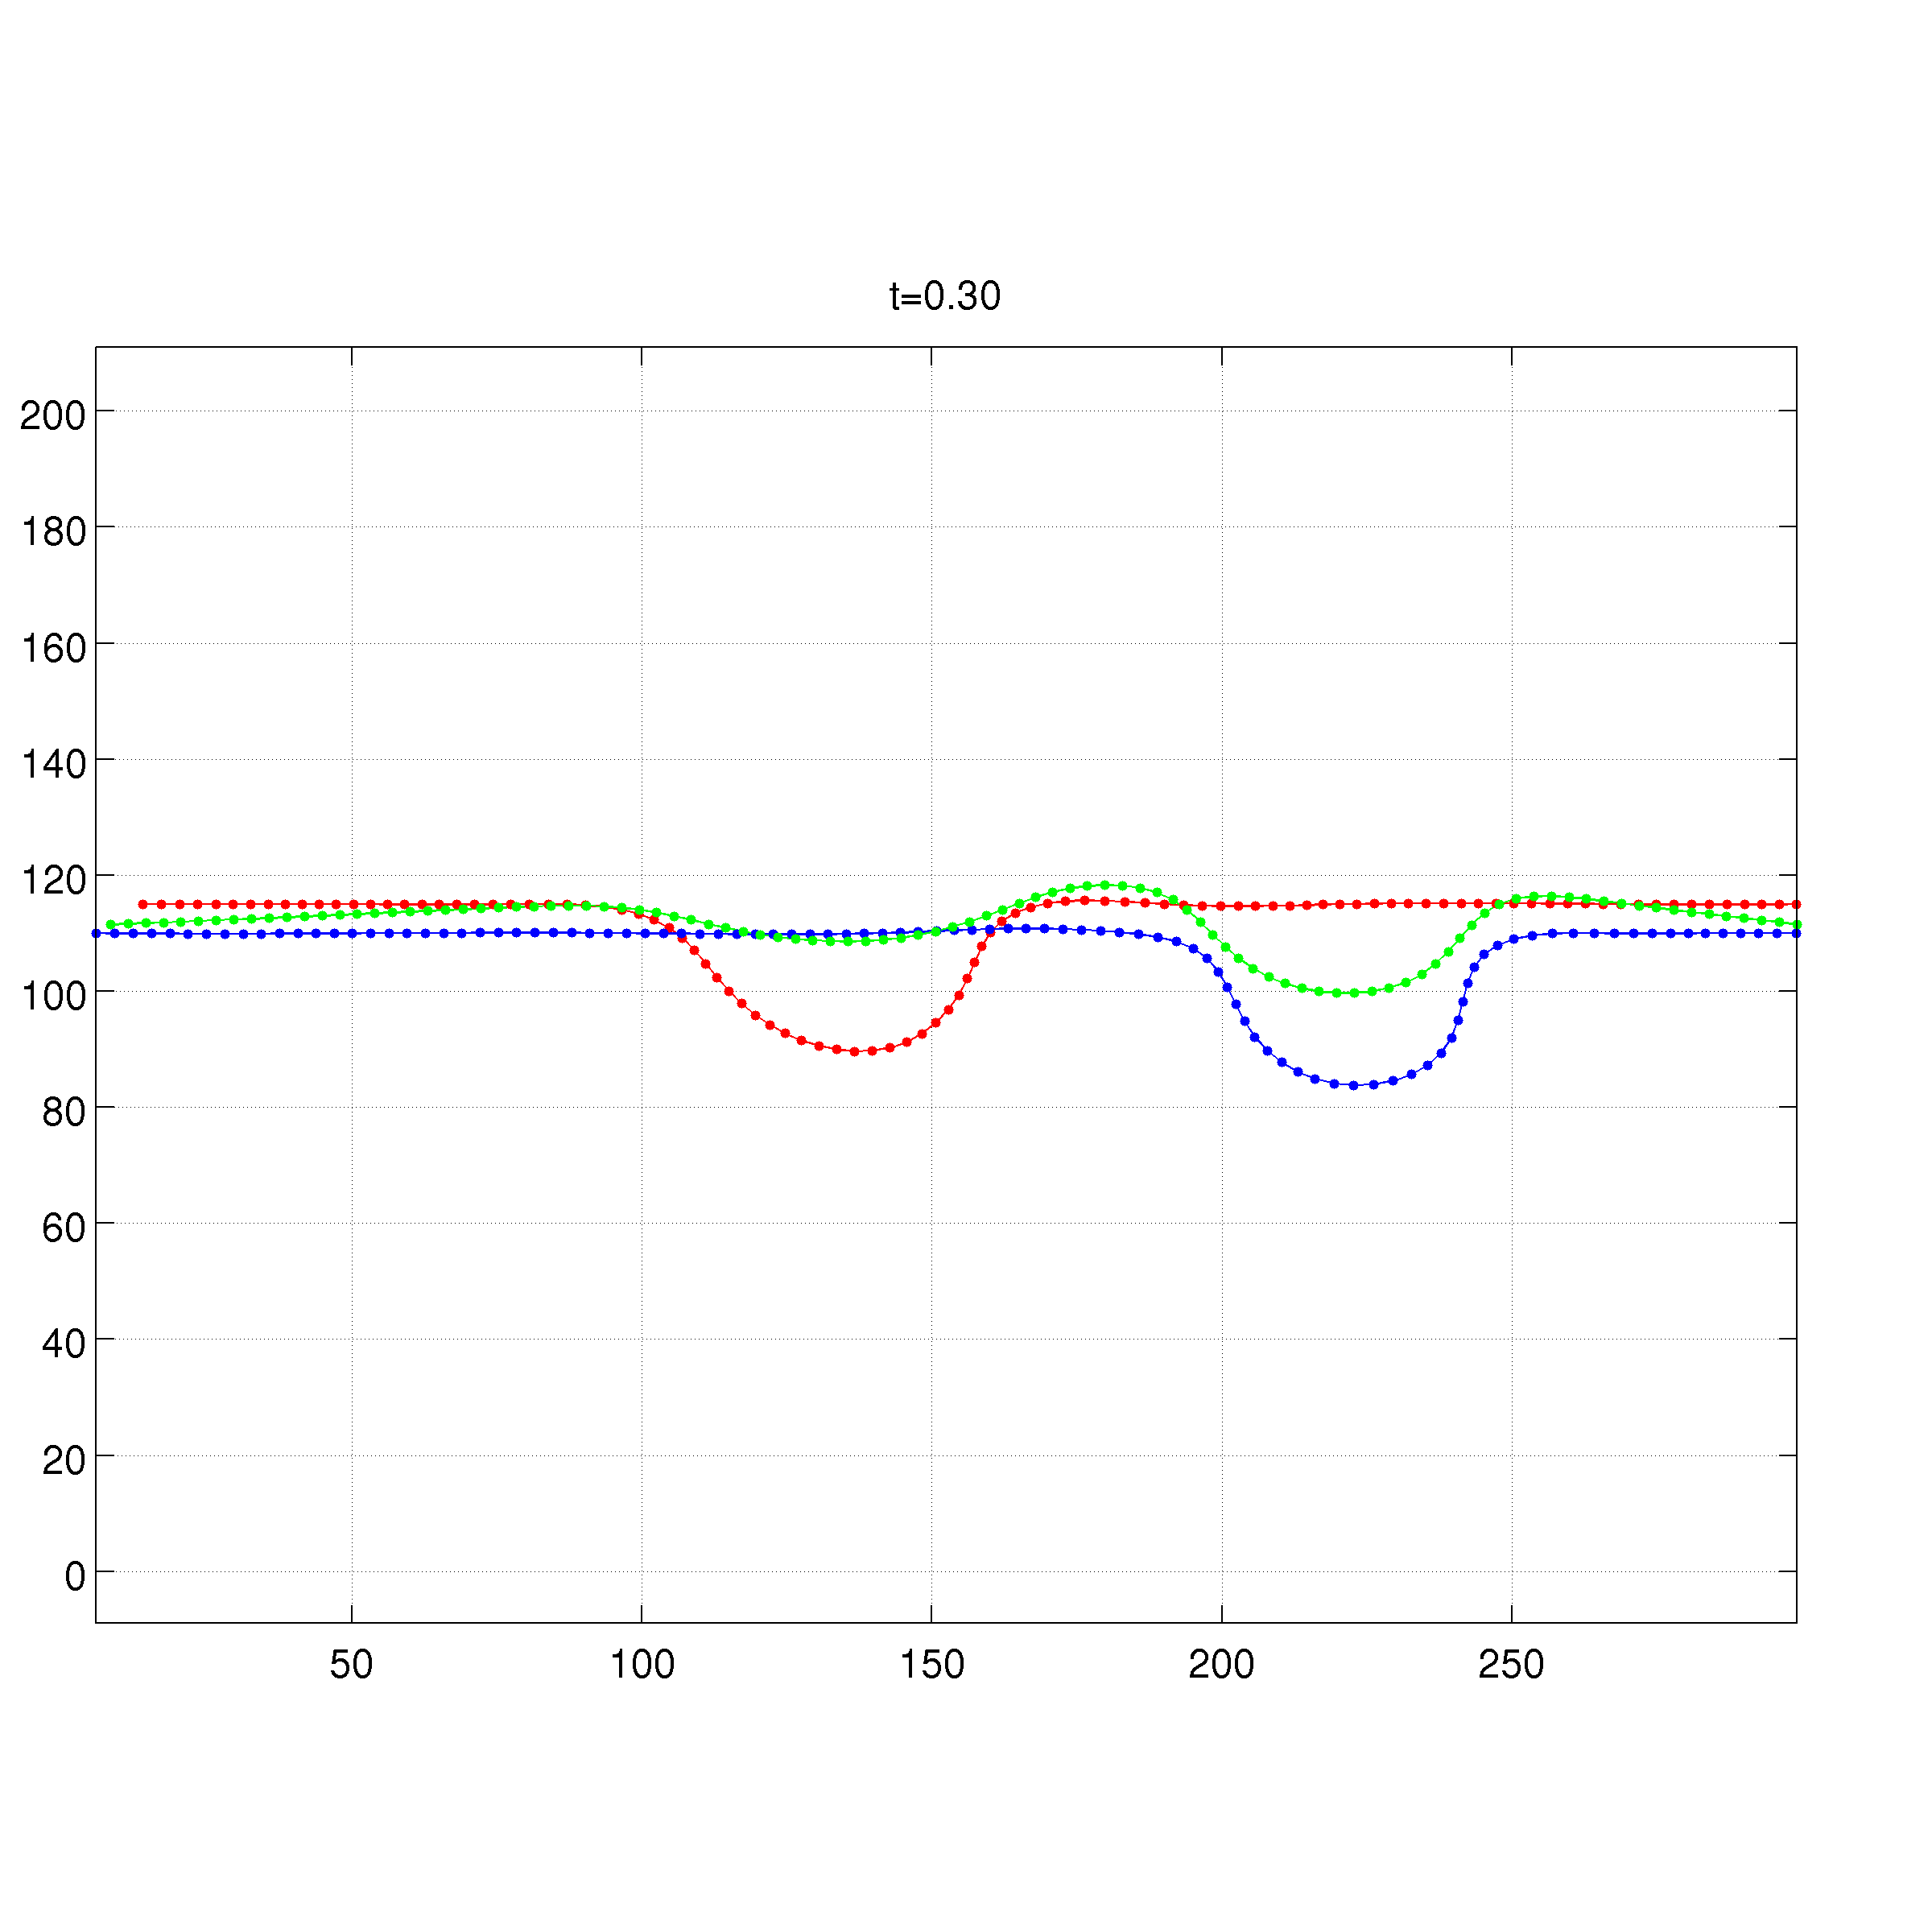
\includegraphics[width=\anchocuatro]{\chapFiveDir/curves/letter_u/animation/interp_0.30.png}
	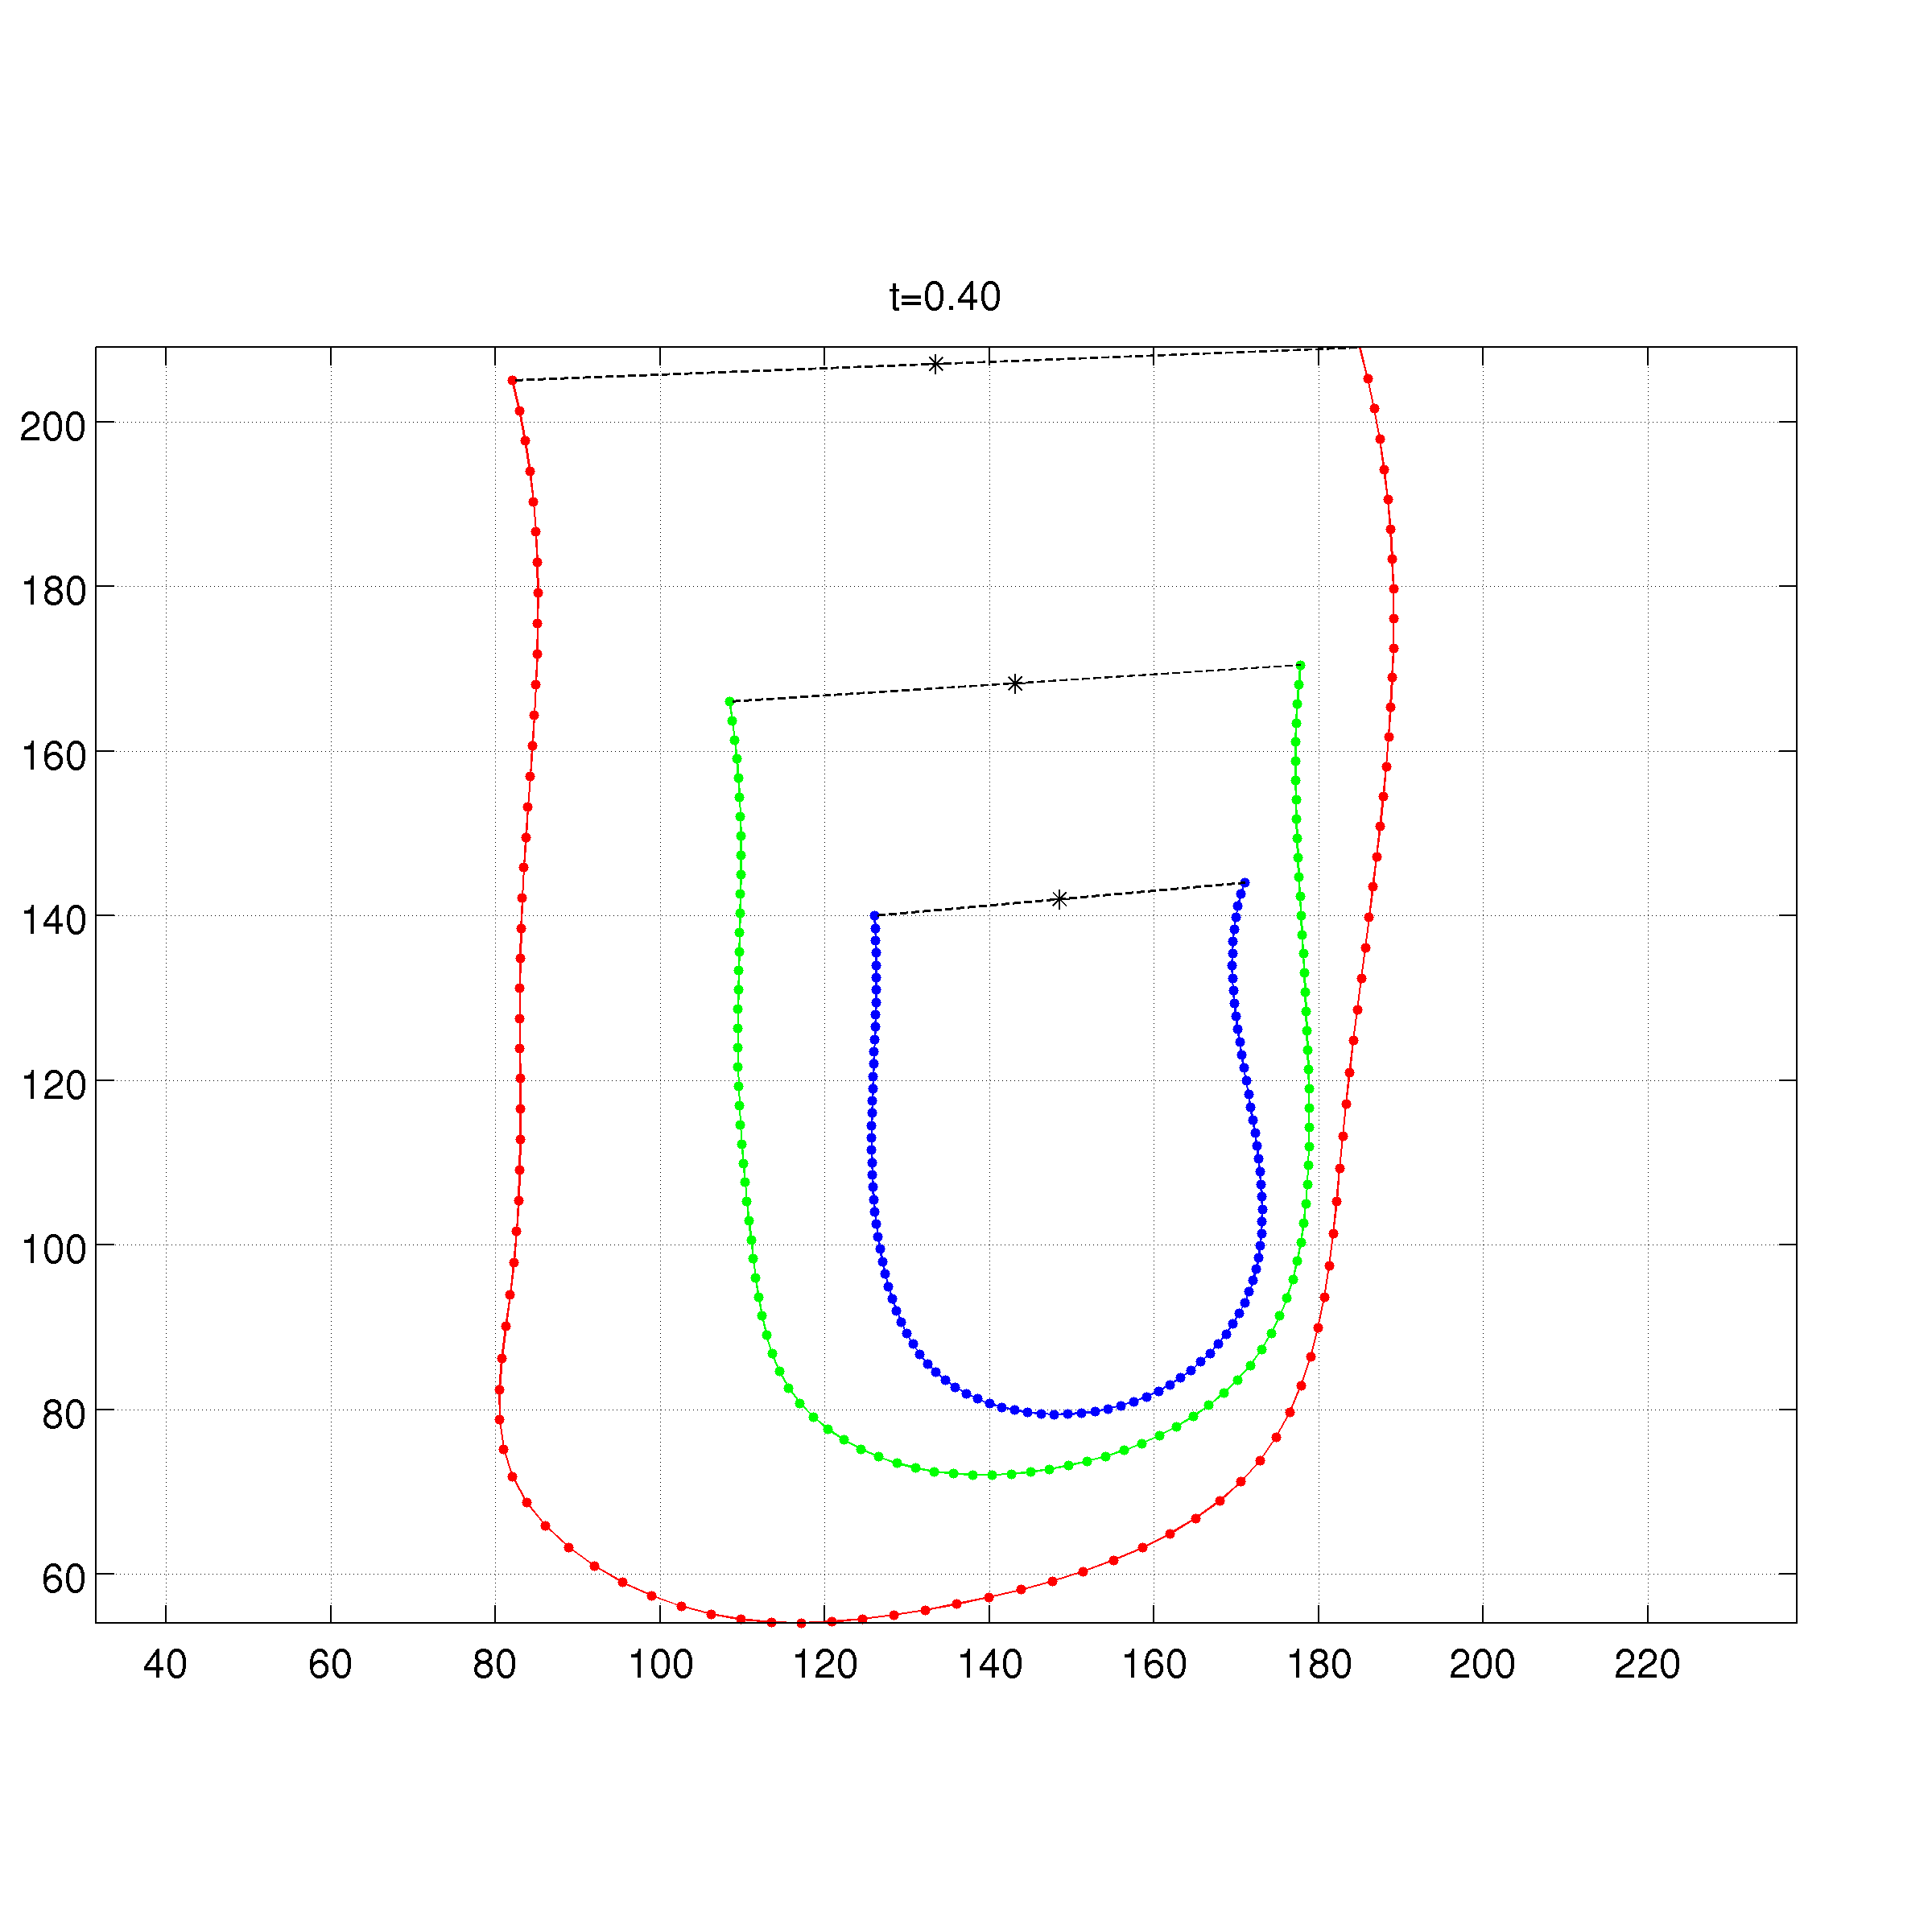
\includegraphics[width=\anchocuatro]{\chapFiveDir/curves/letter_u/animation/interp_0.40.png}
	\includegraphics[width=\anchocuatro]{\chapFiveDir/curves/letter_u/animation/interp_0.50.png}\\
	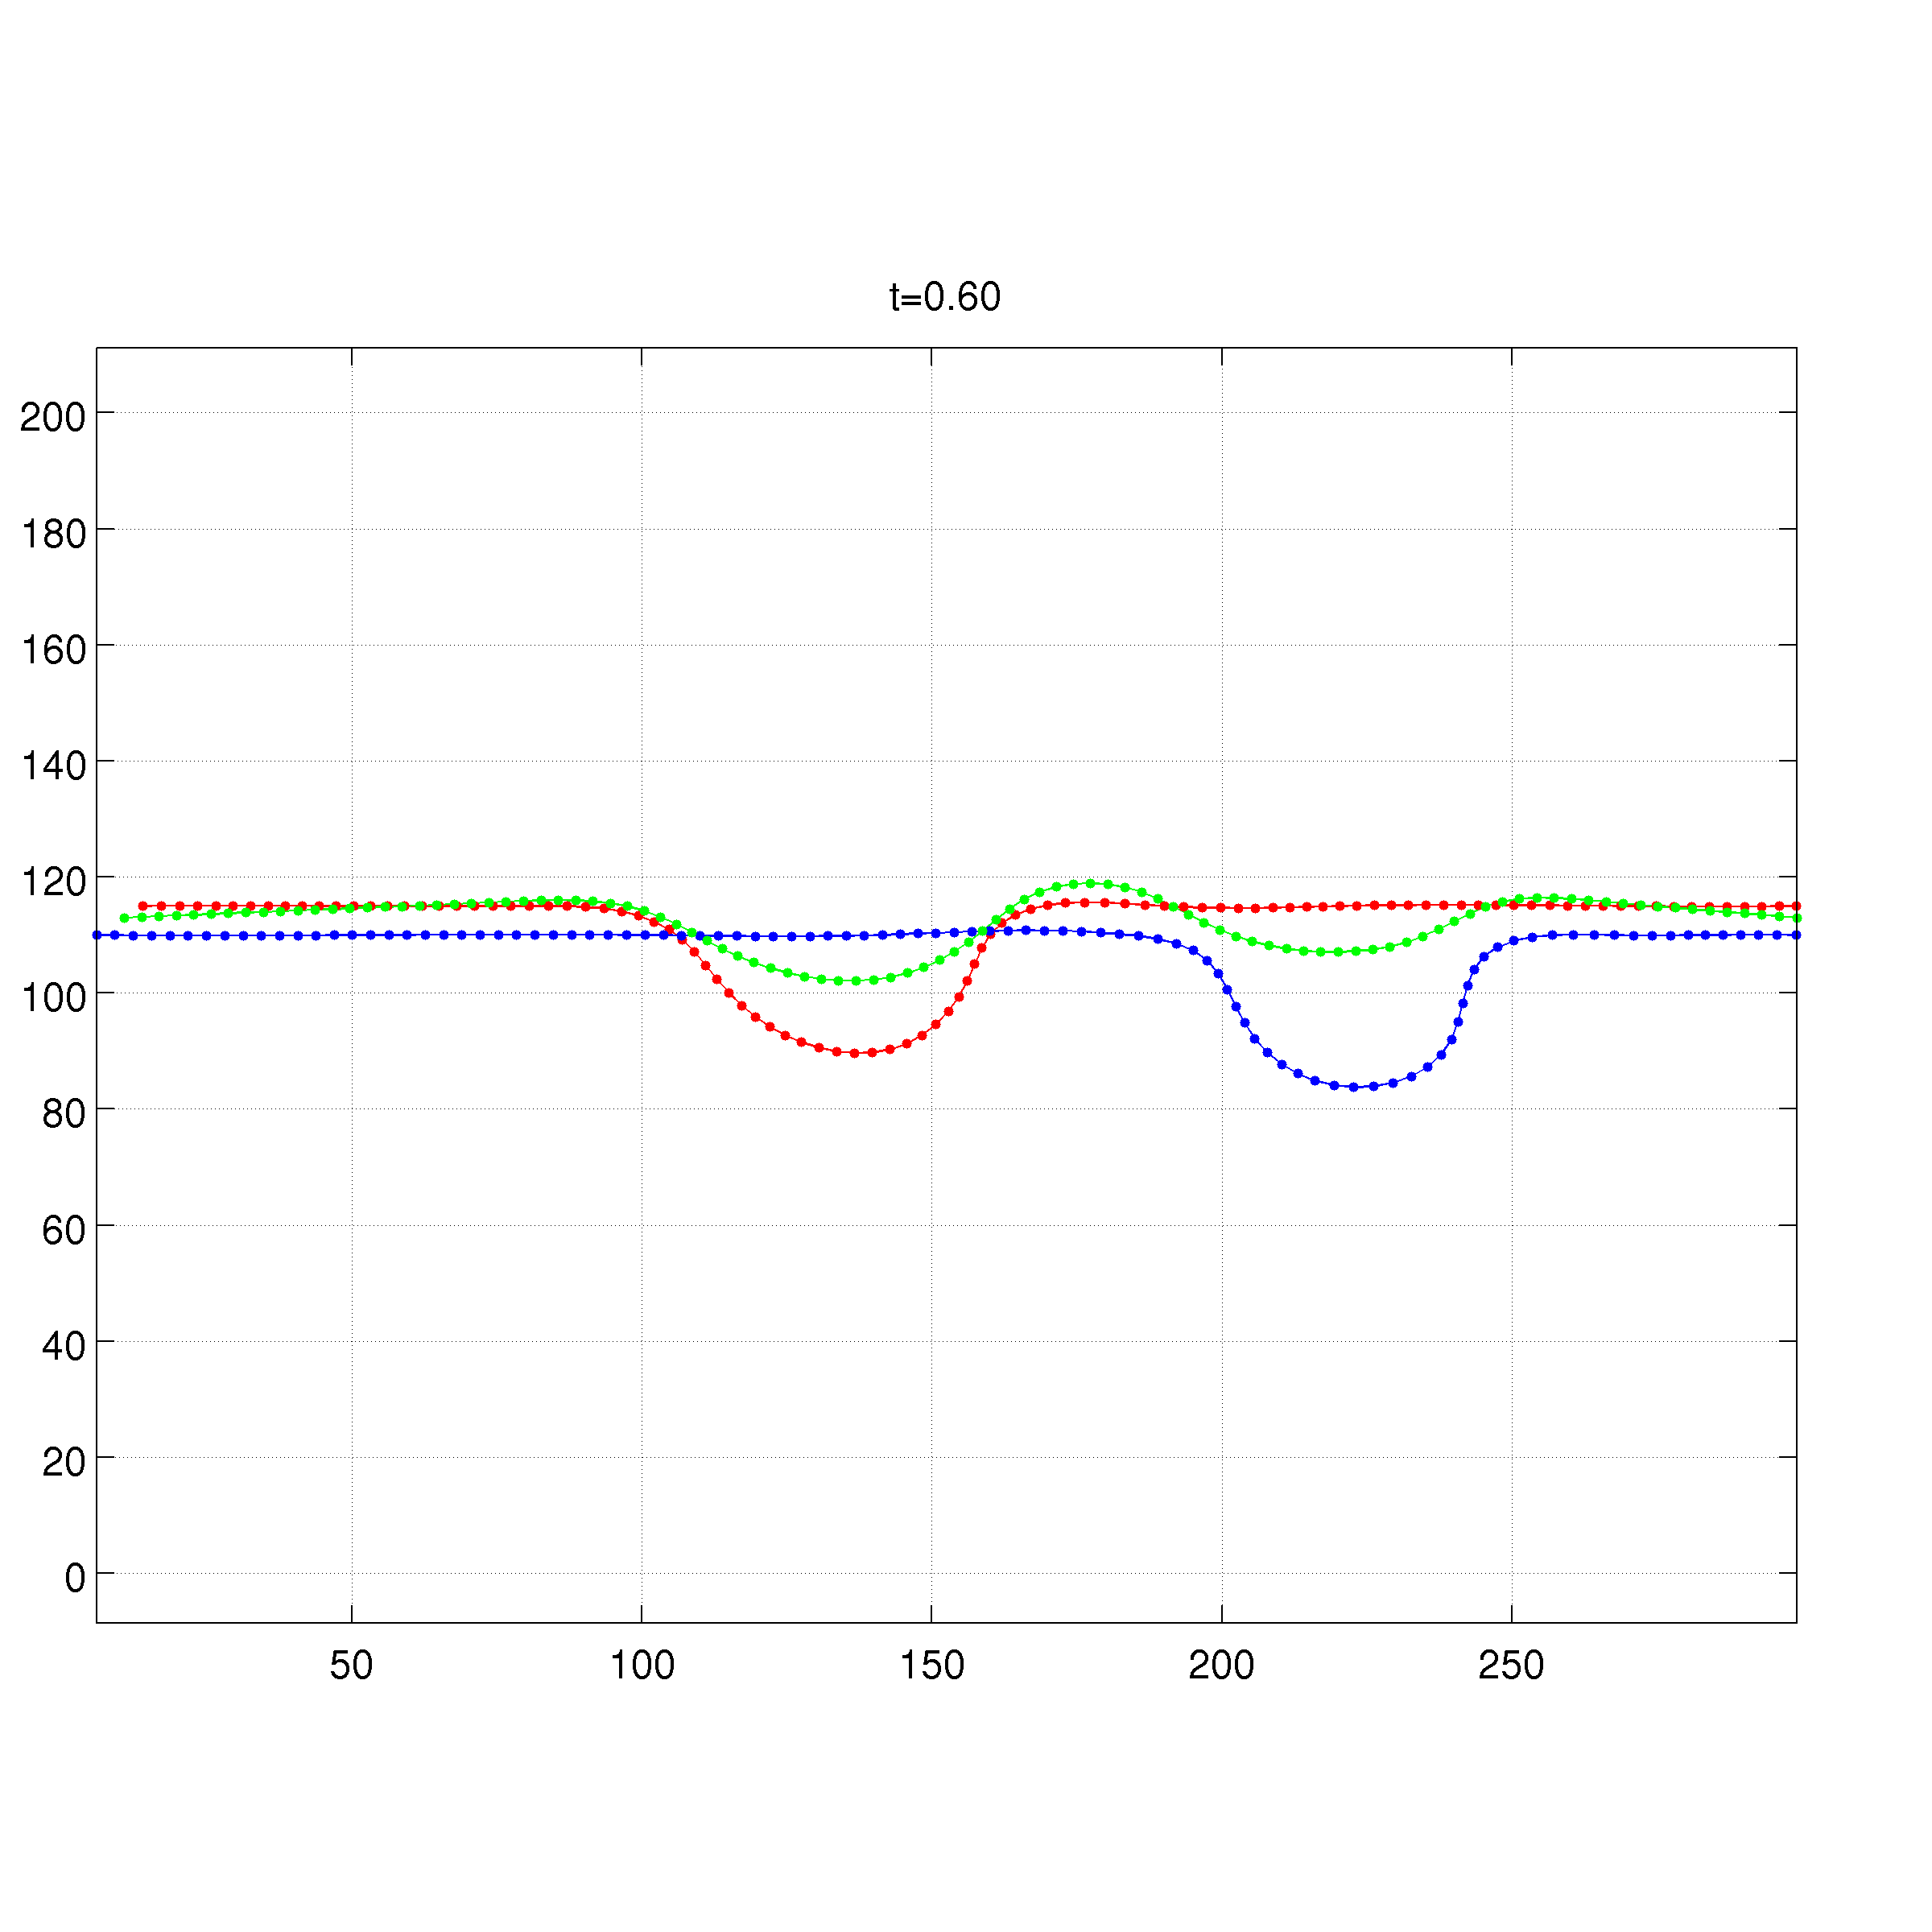
\includegraphics[width=\anchocuatro]{\chapFiveDir/curves/letter_u/animation/interp_0.60.png}
	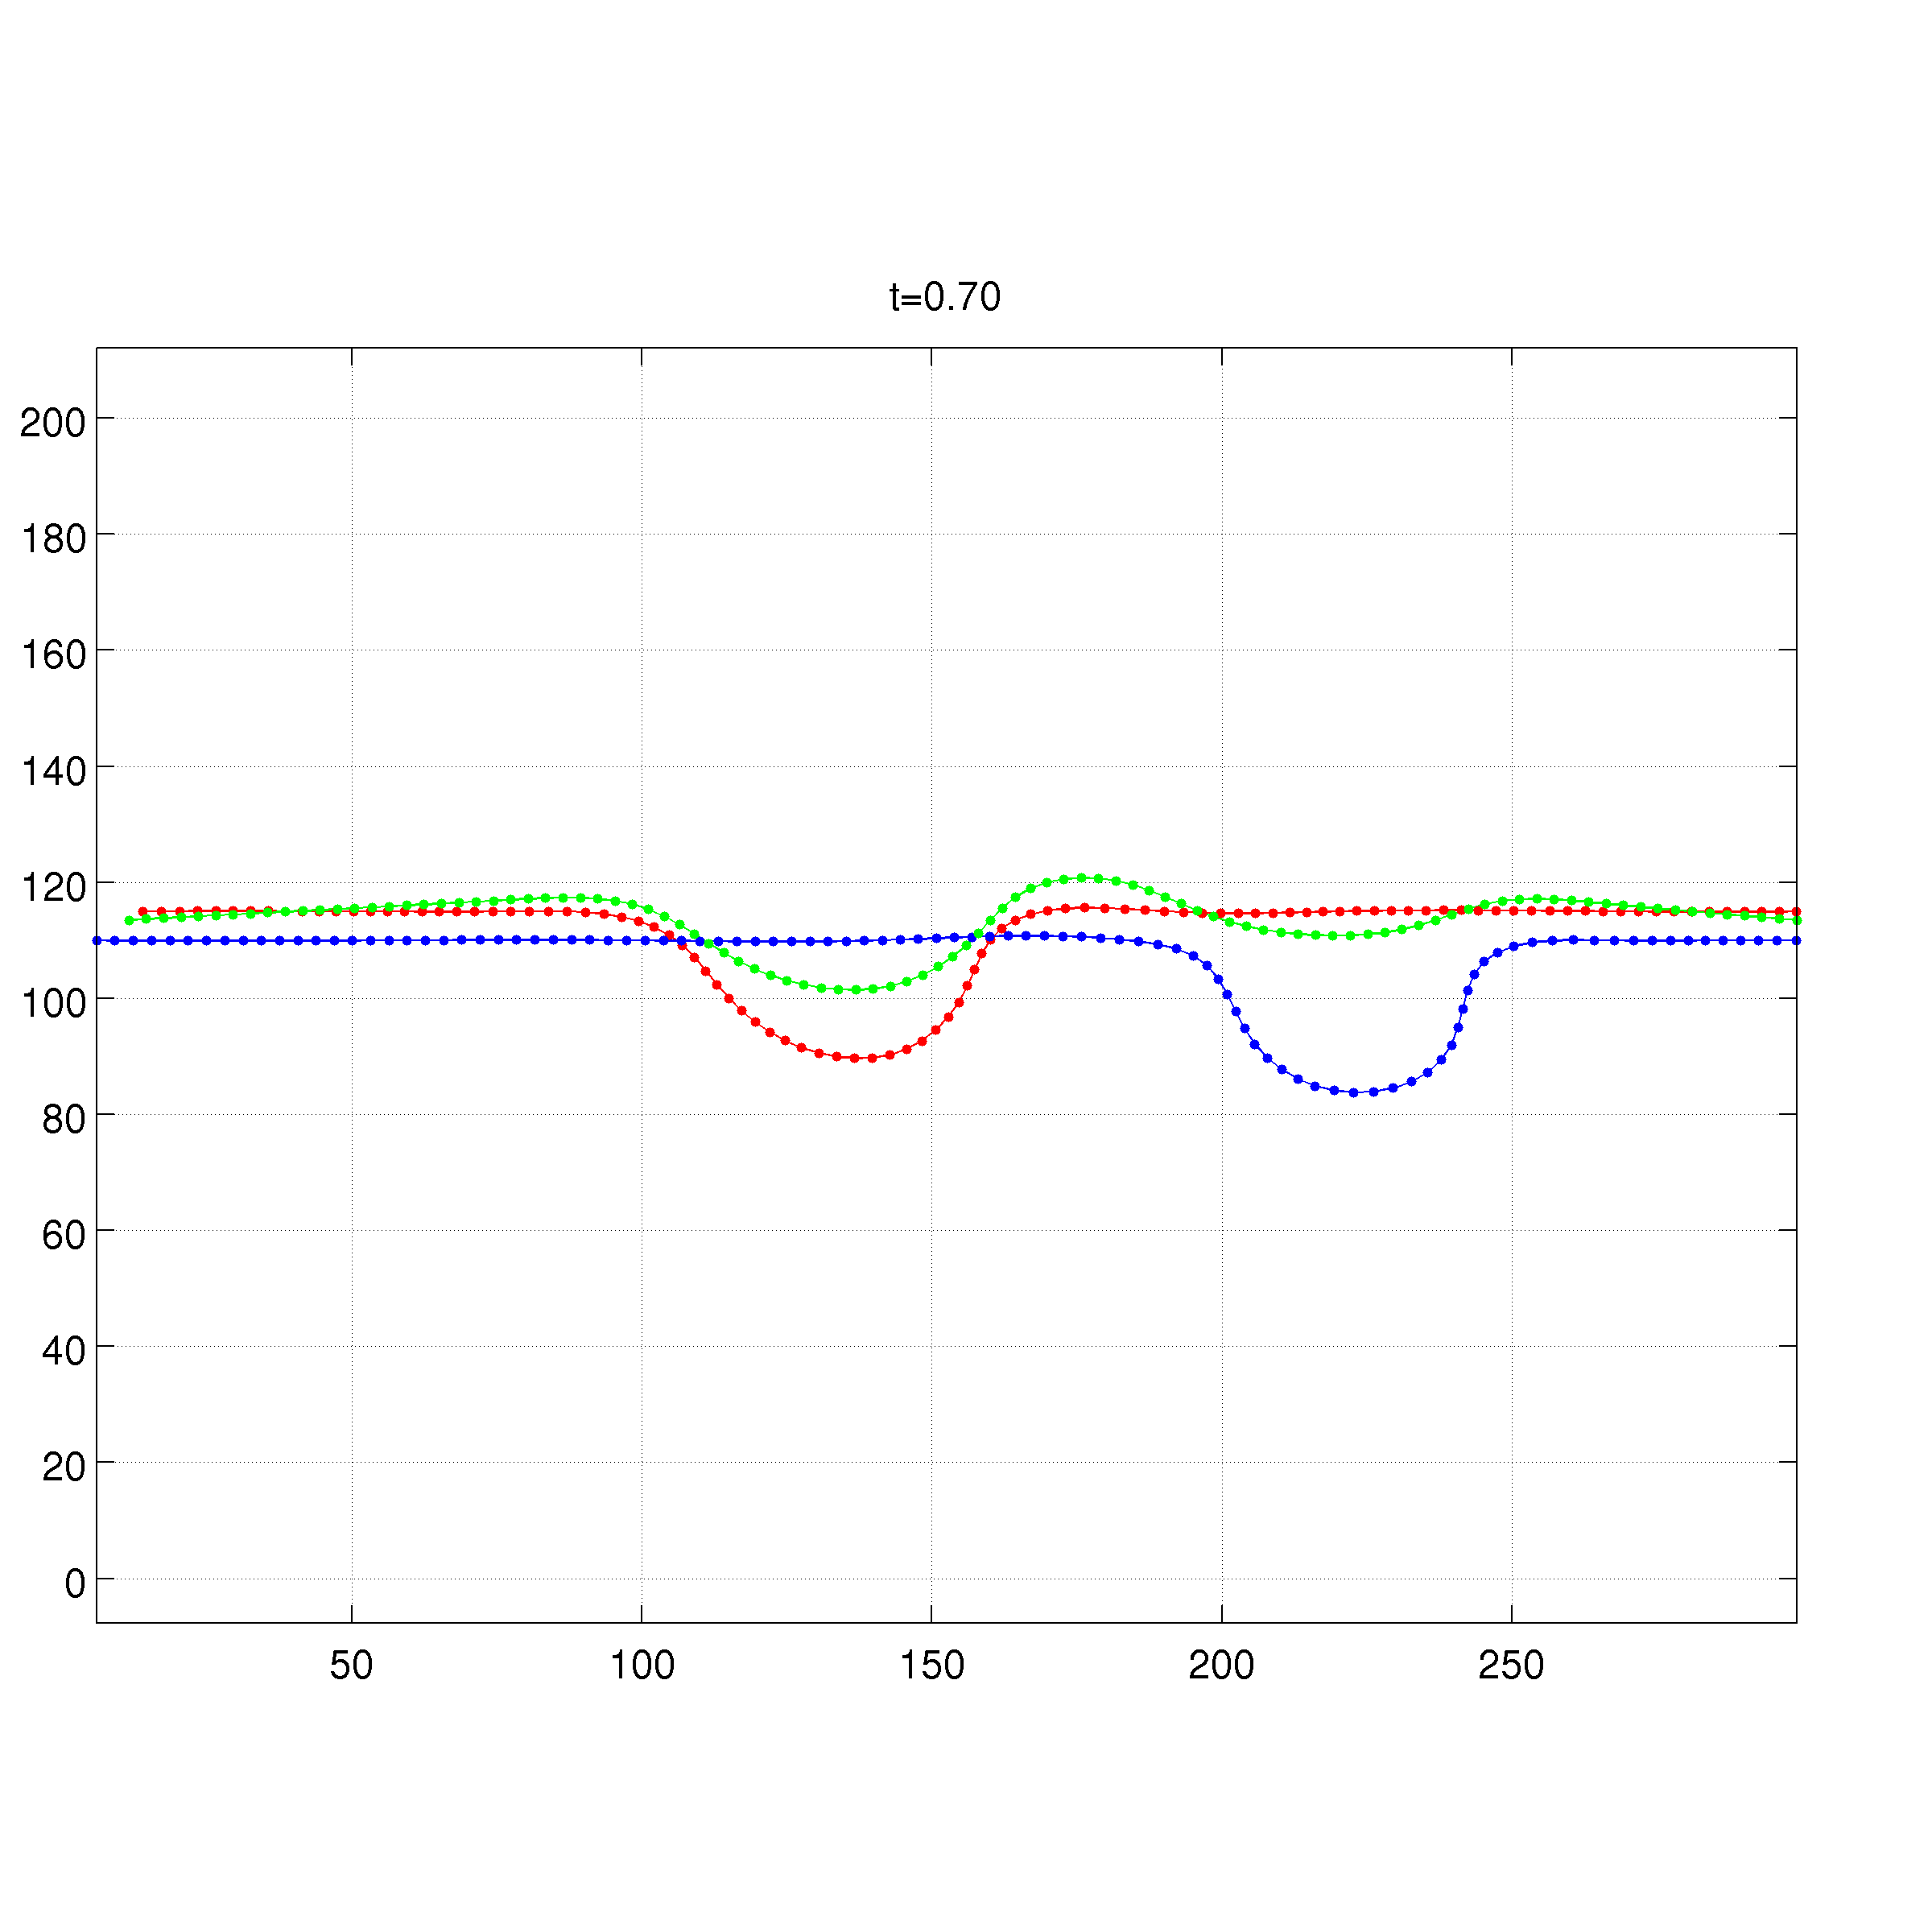
\includegraphics[width=\anchocuatro]{\chapFiveDir/curves/letter_u/animation/interp_0.70.png}
	\includegraphics[width=\anchocuatro]{\chapFiveDir/curves/letter_u/animation/interp_0.80.png}
	\includegraphics[width=\anchocuatro]{\chapFiveDir/curves/letter_u/animation/interp_0.90.png}
	\caption{Example 2: Curvature interpolation of two hand-drawn U-letters at intermediate times \mbox{[0.2 0.3 0.4 0.5 0.6 0.7 0.8 0.9]}. Red: Input curve $C_1$. Blue: Input curve $C_2$. Green: interpolated curve $C_i$. }
	\label{fig:curve_interpolation:results:letter_u:animation}
\end{figure}	


\section{Discussion}\label{sec:curve_interpolation:discussion}

In this chapter we reviewed and reproduced a curve interpolation technique based on the idea of separating intrinsic and extrinsic properties of the curve. Intrinsic description is constructed using curvature signatures and extrinsic properties are described using a rigid transform.
The main contributions of this work are:
\begin{itemize}
	\item Reproducing the proposed technique and validating author's claims. In this sense, we verified that the curvature transform is a good way to describe the curve, and it is very useful for the interpolation and morphing tasks.
	\item Testing an alternative implementation of the algorithm based on numerical integration. The authors of the original work proposed a combination of analytical and numerical approach, while we used a purely numerical approach. This could be an advantage when we have no analytical formulae for the curves to be interpolated.
	We have also carried out a deeper analysis of the specification of the numerical schemes used and their effects on the results. 
	\item Exploring the possibility of replacing point-wise curvature interpolation by Dynamic Time Warping in order to handle the case of curves with similar shape but different in phase.
	\item Providing a careful implementation of the algorithm and making it publicly available. Our implementation is completely performed using simple components, the only external tools used are Matlab's Runge-Kutta routines, but we also provide our own integration schemes. This makes the code completely portable and reproducible.
	\item Providing an online demo where users can upload their own curves and test the algorithm. This helps improving reproducibility by removing obstacles for the researchers to test these algorithms. This demo allows the usage of arbitrarly data, and avoids compatibility, compilation and versioning problems.
	\item Applying the proposed algorithm to the case of curves represented as control points. We applied the algorithm to a case that was not contemplated in the original proposal. We proposed minor changes to extend the technique to this scenario and showed that it works correctly.
\end{itemize}

While the results are interesting and useful for the purpose of this thesis, there are some points that could be improved
\begin{itemize}
	\item The implemented a version of the algorithm only works with open curves. The extension to closed curves is proposed in the original work, and it is very straightforward, but it was out of the scope of this work. 
	\item The same applies to piecewise interpolation of curves. As it is not important for our application, we didn't reproduce that part, but this could be interesting for other computer graphics applications.
\end{itemize}

\subsection{Future Work}

In the first place, we are interested in implementing the parts of the paper that were left out in this work, mainly working with closed curves and piecewise interpolated curves.
Second, and most important, this curvature representation has proven a great potential to be used as a descriptor of the curve, for the task of interpolation. But there are other tasks that could take advantage of meaningful curve descriptors, for example for classification and stabilization tasks. As an example, we are interested in using it as a filtering technique to remove artifacts in facial features tracking.

\appendix
\section{Algorithm's pseudocode}

\begin{figure}[h]
	\centering
	\shadowbox{
		\begin{minipage}{14cm}
			The \verb|curve| data type implemented in the source code is defined with the following fields.\\
			Basic attributes:
			\begin{itemize}
				\item \verb|p|: integer, number of points of the curve
				\item \verb|s|: $1 \times p$, parameter value
				\item \verb|x|: $2 \times p$, position
			\end{itemize}
			
			Derived attributes:
			\begin{itemize}
				\item \verb|x_0|: $2\times1$, start point. $X_o \in \mathbb{R}^{2}$
				\item \verb|x_f|: $2 \times 1$, end point. $X_f \in \mathbb{R}^{2}$
				\item \verb|r|: double, ratio of scaling
				\item \verb|l|: double, length of the curve
				\item \verb|lc|: double, length of the cord defined by start and end point
				\item \verb|theta|: double, initial angle
				\item \verb|G|: $2\times1$, middle point of the cord
			\end{itemize}
			
			Differential magnitudes:
			\begin{itemize}
				\item \verb|n|: $2 \times (p-1)$, normal
				\item \verb|c|: $1 \times p$, curvature
				\item \verb|v|: $2 \times (p-1)$, velocities
				\item \verb|at|: $1 \times p$, angle of the tangent vector
				\item \verb|phi|: $1 \times p$, angle
			\end{itemize}
		\end{minipage}
		\cornersize{.1}
	}
	\caption{Description of the \emph{curve} data type.}
	\label{fig:algo:image_interpolation:curve_interpolation:data_type}
\end{figure}


\RestyleAlgo{ruled}

\begin{algorithm}[hbt!]
	\caption{curve\_main\_curvature\_interpolation}
	\KwIn{polyline filenames $poly1\_fname$ and $poly2\_fname$, time increment $dt$ [optional]}
	
	\Comment{1.-CONFIGURATION}
	\Comment{initialize configuration variables and create output folder}
	$ind\_polyline \leftarrow 1$ \Comment*[r]{Use first curve of each input, since the code supports arrays of curves}
	$dt \leftarrow 0.5$ \Comment*[r]{set default value, if not set}
	
	\Comment{2.-READ INPUT}
	$lines1 \leftarrow read\_curve(poly1\_fname)$ \Comment*[r]{read first curve}
	$poly \leftarrow lines1[ind\_polyline]$\;
	$[c1\_scaled, c1, c11] \leftarrow curve\_polyline\_prepare\_for\_interpolation(poly)$ \Comment*[r]{convert polyline to curve object}
	$lines2 \leftarrow read\_curve(poly2\_fname)$ \Comment*[r]{read second curve}
	$poly2 \leftarrow lines2[ind\_polyline]$\;
	$[c2\_scaled, c2, c22] \leftarrow curve\_polyline\_prepare\_for\_interpolation(poly)$ \Comment*[r]{convert polyline to curve object}
	$[xx1,xx2] \leftarrow sequence\_regenerate\_2(c1\_scaled,c2\_scaled)$ \Comment*[r]{resample curves to the same grid}
	
	\Comment{3.-INTERPOLATE}
	$x_0 \leftarrow dt*c1\_scaled[x_0]+(1-dt)*c2\_scaled[x_0]$\;
	$L \leftarrow dt*c1[l]+(1-dt)*c2[l]$\;
	$phi\_0 \leftarrow 0$\;
	$xi\_angle \leftarrow curve\_interpolate\_angle(xx1, xx2, L, dt, x\_0, phi\_0)$\;
	$xi\_angle \leftarrow curve\_fill\_data(xi\_angle, 0)$ \Comment*[r]{update parameters of the curve}
	$xi\_extrin \leftarrow curve\_interpolate\_extrinsic(xi\_angle, c1, c2, dt)$\;
	$xi\_extrin \leftarrow curve\_fill\_data(xi\_extrin, 0)$ \Comment*[r]{update parameters of the curve}
	$curve\_get\_bounding\_box\_of\_two\_curves(...)$, $curve\_rect\_union(...)$ \Comment*[r]{determine bounding boxes}
	%$rect1 \leftarrow curve\_get\_bounding\_box\_of\_two\_curves(c1[x], xi\_extrin[x])$
	% %$rect1 \leftarrow curve\_get\_bounding\_box\_of\_two\_curves(c1[x], xi\_extrin[x])$
	% %$rect2 \leftarrow curve\_get\_bounding\_box\_of\_two\_curves(c2[x], xi\_extrin[x])$
	% %$rect\_union \leftarrow curve\_rect\_union(rect1, rect2)$ \Comment{determine max bounding boxes}
	% %$[ax\_lim, x\_lims, y\_lims] \leftarrow curve\_compute\_axis\_limits(rect\_union)$ \Comment{compute margins of plots}
	
	\Comment{4.-MORPH}
	$ci\_angle\_array \leftarrow curve\_morph\_angle(xx1, xx2, c1.l, c2.l, dt, ax\_lim, opt.save)$ \Comment*[r]{interpolate using angles}
	$ci\_curvature\_array \leftarrow curve\_morph\_curvature(xx1, xx2, dt, ax\_lim)$  \Comment*[r]{interpolate using curvature}
	
	\Comment{5.-PLOT}
	\For {$k \gets 1$ to $length(ci\_angle\_array)$}{
		\Comment{plot the $k$th step of $curve\_angle$ $ci\_angle\_array[k]$}
		\Comment{plot the $k$th step of $curve\_curvature$ $ci\_angle\_curvature\_array[k]$}
	}
\end{algorithm}

\begin{algorithm}[hbt!]
	\caption{curve\_polyline\_prepare\_for\_interpolation}
	\KwIn{polyline object ($poly$), execution type ($type$)}
	\KwOut{scaled curve $c1\_scaled$, upsampled and reparametrized curve $c1$, upsampled curve $c11$}
	$c11 \leftarrow$ generate upsampled curve from $poly$ \Comment{$polyline\_to\_curve\_2(...)$}
	$c1 \leftarrow$ reparametrize $c11$ to arc lenght \Comment{$curve\_reparametrize(...)$}
	\Comment{compute normals and update angle signatures of $c1$}
	$c1.c \leftarrow [c1.c, c1.c(1)]$\;
	\Comment{update parameters of $c1$}
	$c1\_scaled \leftarrow$ scale curve $c1$ to have length 1\;
	\Comment{update parameters of $c1\_scaled$}
\end{algorithm}

\begin{algorithm}[hbt!]
	\caption{curve\_interpolate\_angle}
	\KwIn{curve ($c1$), curve ($c2$), (\tcom{$L$}), time ($t$), starting point ($x\_0$), angle ($phi\_0$)}
	\KwOut{interpolated curve ($xi$)}
	% \Comment{Interpolate two curves using their angle signatures}
	\Comment{Copy $c1.s$ and $x\_0$ to $xi$}
	% $xi.s \leftarrow c1.s$\;
	% $xi.x\_0 \leftarrow x\_0$\;
	$xi.at \leftarrow t*c1.at+(1-t)*c2.at$\;
	$xi.phi \leftarrow t*c1.phi+(1-t)*c2.phi$\;
	$xi.x \leftarrow curve\_angle\_reconstruct(xi,x\_0,L)$ \Comment{Reconstruct the curve}
\end{algorithm}

\begin{algorithm}[hbt!]
	\caption{curve\_interpolate\_extrinsic}
	\KwIn{curve ($xi$), curve ($x1$), curve ($x2$), time ($t$), execution type ($type$)}
	\KwOut{interpolated curve ($xif$)}
	\Comment{\tcom{here we are assuming that the curve was interpolated using curvature and starting point x\_0 and angle phi\_0}}
	\Comment{Copy arguments from $xi$ to $xif$}
	\Comment{Interpolate starting and ending points}
	
	$xd.G \leftarrow t*x1.G+(1-t)*x2.G$\;
	\Comment{compute rotation angle}
	\If {$abs(x1.theta-x2.theta)< \pi$}
	{$xd.theta \leftarrow x2.theta+(x1.theta-x2.theta)/2$}
	\Else
	{$xd.theta \leftarrow x2.theta+2\pi-(x1.theta-x2.theta)/2$}
	$xd.lc \leftarrow t*x1.lc+(1-t)*x2.lc$\;
	$dir \leftarrow -[cos(xd.theta) ; sin(xd.theta)]$\;
	$xd.x\_0 \leftarrow xd.G-xd.lc*dir/2$\;
	$xd.x\_f \leftarrow xd.G+xd.lc*dir/2$\;
	$Ci \leftarrow xi.G$\;
	$Cd \leftarrow xd.G$\;
	
	\Comment{compute ratio of the scaling}
	\Comment{compute rotation angle, construct rotation matrix and finally rotate the curve}
	
	\Comment{\tcom{Falta especificar}}
\end{algorithm}

\begin{algorithm}[hbt!]
	\caption{curve\_morph\_angle}
	\KwIn{curve 1 $c1$, curve 2 $c2$, length of curve 1 $l1$, length of curve 2 $l2$, time increment $dt$, axes limits $ax\_lim$, save plots $save$}
	\KwOut{interpolated curves $ci\_array$}
	
	\Comment{plot input curves $c1$ and $c2$ according to $save$}
	$ci\_array \leftarrow cell(1,1)$\;
	$phi\_0 \leftarrow 0$\;
	\For {$t \gets 0$ \KwTo $1$ \KwBy $dt$}{
		% \Comment{interpolate curves for each step}
		$x\_0 \leftarrow t*c1.x\_0+(1-t)*c2.x\_0$\;
		$L \leftarrow t*l1+(1-t)*l2$\;
		$xi\_angle \leftarrow$ $curve\_interpolate\_angle(c1,c2,L,t,x\_0,phi\_0)$ \Comment*[r]{interpolate by angle}
		\Comment{update parameters of $xi\_angle$}
		
		$[xi\_extrin] \leftarrow curve\_interpolate\_extrinsic(xi\_angle,c1,c2,t)$\;
		$xi \leftarrow$ update parameters of $xi\_extrin$\;
		$xi.t \leftarrow t$\;
		
		\Comment{append $xi$ to $ci\_array$}
	}
\end{algorithm}

\begin{algorithm}[hbt!]
	\caption{curve\_morph\_curvature}
	\KwIn{curve $c1$, curve $c2$, time increment $dt$, axes limits $ax\_lim$ [optional], type of execution $type$ [optional]}
	\KwOut{interpolated curves $ci\_array$}
	
	$xi.s \leftarrow c1.s$\;
	$pt \leftarrow 0.2$\;
	\Comment{plot input curves $c1$ and $c2$ using $ax\_lim$, according to $save$}
	$ci\_array \leftarrow cell(1,1)$\;
	
	\For{$t \gets 0$ \KwTo $1$ \KwBy $dt$}{
		% \Comment{interpolate curves for each step}
		$xi \leftarrow curve\_interpolate\_curvature\_full(c1, c2, t, opt.type)$\;
		$xi.t \leftarrow t$\;
		\Comment{append $xi$ to $ci\_array$}
	}
\end{algorithm}

\bibliographystyle{siam}
\bibliography{../publications/tools/journal_list_long,../publications/tools/references,../publications/tools/hierarchical_segmentation,../publications/tools/bib_enric,../publications/tools/reproducibility,../publications/tools/varios,../publications/tools/graph_theory,../publications/tools/slow_motion.bib,../publications/tools/computer_graphics.bib,../publications/tools/curves.bib}

\end{document}